\documentclass[12pt,twoside,a4paper]{book}


%\includeonly{biophysics/biophysics}
%\includeonly{cardiac_electrophysiology/cardiac_electrophysiology}
%\includeonly{electrophysiology/electrophysiology}

%
% Macros.tex - global macros file
%
% Created:
%   10 September 1996
%
% Updates:
%   Leo Cheng 31 May 1998, macros for DES software names
%   Leo Cheng 19 August 1998, added units for grams and kg
%   Leo Cheng 18 January 1999, added units for ohmcm
%   Leo Cheng 17 May 1999, adding modified url package and macros
%   Chris Bradley, 1 Dec 1999, adding \unitseparator.
%   Chris Bradley, 7 September 2000, Changed \lps to \Lps and \mMpLpms etc.
%     to \mmolpLpms etc.
%   Mark Trew, 8 June 2001. Made all macro arguments raised to a power
%     protected by {}, e.g. replaced #2^ with {#2}^.
%   Chris Bradley, 22 Feb 2011. Added svg figure support. 
%   Chris Bradley, 6 August 2014, Differential geometry support.
%   Chris Bradley, 4 July 2017, tidyup for outdated packages.

%
% Necessary packages
%
\usepackage{alltt}
\usepackage[centertags]{amsmath}
\usepackage{amssymb}
\usepackage{amsfonts}
\usepackage{calc}
\usepackage{keyval}
\usepackage{graphicx}
\usepackage{epsfig}
\usepackage{ifthen}
\usepackage{caption}
\usepackage{subcaption}
\usepackage{latexsym}
\usepackage{moreverb}
\usepackage[subfolder,cleanup]{gnuplottex}
\usepackage{xspace}
\usepackage{url}

%
% Allow superimposition of symbols
%
\makeatletter
\newcommand{\superimpose}[2]{%
  {\ooalign{$#1\@firstoftwo#2$\cr\hfil$#1\@secondoftwo#2$\hfil\cr}}}
\makeatother

%
% URL commands
%
\newcommand{\email}     {\begingroup \urlstyle{sf}\Url}
\newcommand{\directory} {\begingroup \urlstyle{sf}\Url}
\newcommand{\file}      {\begingroup \urlstyle{sf}\Url}
\renewcommand{\url}     {\begingroup \urlstyle{sf}\Url}

%
% Software and systmes
%
\newcommand{\OpenCMISS}{\textsf{OpenCMISS}\xspace}
\newcommand{\CMISS}{\textsf{CMISS}\xspace}
\newcommand{\CM}{\textsf{CM}\xspace}       %note upper case to distinguish from centimeters
\newcommand{\CMGUI}{\textsf{CMGUI}\xspace}
\newcommand{\UNEMAP}{\textsf{UnEmap}\xspace}
\newcommand{\FieldML}{\textsf{FieldML}\xspace}
\newcommand{\CellML}{\textsf{CellML}\xspace}
\newcommand{\FAROARM}{\textsf{FARO ARM\xspace}}
\newcommand{\OpenMP}{\textsf{OpenMP\xspace}}
\newcommand{\OpenACC}{\textsf{OpenACC\xspace}}

%
% New commands
%
\newcommand{\Index}[1]{#1\index{#1}}
\newcommand{\subsubsubsection}[1]{\noindent\textbf{#1}}
%\newcommand{\newabbrev}[2]{\newcommand{#1}{#2\xspace}}
%\newcommand{\newabbrevs}[3]{\newcommand{#1}{#2\xspace}\newcommand{#3}{#2s\xspace}}
\newcommand{\clearemptydoublepage}{\newpage{\pagestyle{empty}\cleardoublepage}}
%\newcommand{\newion}[3]{\newcommand{#1}{\ion{#2}{#3}}} % new ion
%\newcommand{\newunit}[2]{\newcommand{#1}{\units{#2}}} % new unit

%
% New enironments
%
\newenvironment{code}[0]{\small\begin{alltt}}{\end{alltt}\normalsize}

%
% Figures etc.
%
\newcommand{\pdftexfigure}[5]{ %
  \begin{figure}[htbp] \centering %
   \ifthenelse{\equal{#5}{}}{ %
      \def\svgwidth{\columnwidth}}{ %
      \def\svgscale{#5} %
    } %
    \input{#1} %
    \ifthenelse{\equal{#2}{}}{ %
      \caption{#3}}{ %
      \caption[#2]{#3} %
      } %
    \label{#4} %
  \end{figure} %
  } % pdftex figure i.e. inkscape svgs
    % e.g. \pdftexfigure{figure}{short caption}{long caption}{label}{scale}
    % or \pdftexfigure{figure}{}{caption}{label}{}

\newcommand{\epstexfigure}[5]{ %
  \begin{figure}[htbp] \centering %
    \ifthenelse{\equal{#5}{}}{ %
      \def\svgwidth{\columnwidth}}{ %
      \def\svgscale{#5} %
    } %
    \input{#1} %
    \ifthenelse{\equal{#2}{}}{ %
      \caption{#3}}{ %
      \caption[#2]{#3} %
    } %
    \label{#4} %
  \end{figure} %
  } % epstex figure i.e. inkscape svgs
  % e.g. \epstexfigure{figure}{short caption}{long caption}{label}{scale}
  % or \epstexfigure{figure}{}{caption}{label}{}
  
\newcommand{\epstexsubfigure}[5]{ %
  \centering %
  \ifthenelse{\equal{#5}{}}{ %
    \def\svgwidth{\columnwidth}}{ %
    \def\svgscale{#5} %
  } %
  \ifthenelse{\equal{#2}{}}{ %
    \subfloat[][#3]{\input{#1}}}{ %
    \subfloat[#2][#3]{\input{#1}} %
  } %
  \label{#4} %
} % epstex sub figure i.e. inkscape svgs
  % e.g. \epstexsubfigure{figure}{short caption}{long caption}{label}{scale}
  % or \epstexsubfigure{figure}{}{caption}{label}{}
  
\newcommand{\gnuplotsubfigure}[8]{ %
  \begin{subfigure}[b]{#5}
    \centering %
    \ifthenelse{\equal{#8}{}}{ %
      \gnuplotloadfile[terminal=pslatex,terminaloptions={color size #7,#7 #6}]{#1}}{ %
      \gnuplotloadfile[terminal=pslatex,terminaloptions={color size #7,#8 #6}]{#1} %
    } %
    \ifthenelse{\equal{#2}{}}{ %
      \caption{#3}}{ %
      \caption[#2]{#3} %
    } %
    \label{#4} %
  \end{subfigure}
} % gnuplot subfigure e.g. \gnuplotsubfigure{file}{short caption}{long caption}{label}{subfigurescale}{fontsize}{gnuplotxsize}{gnuplotysize}
  
\newcommand{\pstexfigure}[5]{ %
  \begin{figure}[htbp] \centering %
    \ifthenelse{\equal{#5}{}}{ %
      \def\svgwidth{\columnwidth}}{ %
      \def\svgscale{#5} %
    } %
    \input{#1} %
    \ifthenelse{\equal{#2}{}}{ %
      \caption{#3}}{ %
      \caption[#2]{#3} %
      } %
    \label{#4} %
  \end{figure} %
  } % pstex figure i.e. inkscape, xfig or gnuplot
    % e.g. \pstexsubfigure{figure}{short caption}{long caption}{label}{scale}
    % or \pstexsubfigure{figure}{}{caption}{label}{}

\newcommand{\pstexsubfigure}[5]{ %
  \begin{subfigure}[b]{0.45\columnwidth} \centering %
    \setkeys{Gin}{width=\columnwidth}
    \input{#1} %
    \ifthenelse{\equal{#2}{}}{ %
      \caption{#3}}{ %
      \caption[#2]{#3} %
    } %
    \label{#4} %
  \end{subfigure} %
} % pstex subfigure i.e. inkscape, xfig or gnuplot
    % e.g. \pstexsubfigure{figure}{short caption}{long caption}{label}{scale}

\newcommand{\epsfigure}[4]{ %
  \incgrfigure{}{#1}{#2}{#3}{#4}
  } % eps figure
    % e.g. \epsfigure{epsfig options}{short caption}{long caption}{label}
    % or \epsfigure{epsfig options}{}{caption}{label}

\newcommand{\incgrfigure}[5]{ %
  \begin{figure}[htbp] \centering %
    \includegraphics[#1]{#2} %
    \ifthenelse{\equal{#3}{}}{ %
      \ifthenelse{\equal{#4}{}}{
        {}{ %
          \caption{#4}
        }}{
        \caption[#3]{#4} %
      }} %
    \label{#5} %
  \end{figure} %
  } % include graphics figure
    % e.g. \incgrfigure{height/width options}{epsfig options}{short caption}
    %                  {long caption}{label}
    % or \incgrfigure{height/width options}{epsfig options}{}{caption}{label}

%
% Formats for references to equations, tables etc.
%
\newcommand{\appendref}[1]{Appendix~\ref{#1}} % Appendix reference
\newcommand{\Appendref}[1]{Appendix~\ref{#1}} % Appendix reference
\newcommand{\appendrefs}[2]{Appendices~\ref{#1} and~\ref{#2}} % Appendices ref.
\newcommand{\Appendrefs}[2]{Appendices~\ref{#1} and~\ref{#2}} % Appendices ref.
\newcommand{\appendthrurefs}[2]{Appendices~\ref{#1}--\ref{#2}} % Appendices--
\newcommand{\Appendthrurefs}[2]{Appendices~\ref{#1}--\ref{#2}} % Appendices--
\newcommand{\bref}[1]{(\ref{#1})} % bracketed () reference
\newcommand{\baubref}[1]{(\subref{#1})} % bracketed () subreference
\newcommand{\chapref}[1]{Chapter~\ref{#1}} % Chapter reference
\newcommand{\Chapref}[1]{Chapter~\ref{#1}} % Chapter reference
\newcommand{\chaprefs}[2]{Chapters~\ref{#1} and~\ref{#2}} % Chapters reference
\newcommand{\Chaprefs}[2]{Chapters~\ref{#1} and~\ref{#2}} % Chapters reference
\newcommand{\chathrurefs}[2]{Chapters~\bref{#1}--\bref{#2}} % Chapters-- ref.
\newcommand{\Chathrurefs}[2]{Chapters~\bref{#1}--\bref{#2}} % Chapters-- ref.
\newcommand{\eqnref}[1]{Equation~\bref{#1}} % Equation reference
\newcommand{\Eqnref}[1]{Equation~\bref{#1}} % Equation reference
\newcommand{\eqnrefs}[2]{Equations~\bref{#1} and~\bref{#2}} % Equations ref.
\newcommand{\Eqnrefs}[2]{Equations~\bref{#1} and~\bref{#2}} % Equations ref.
\newcommand{\eqnthrurefs}[2]{Equations~\bref{#1}--\bref{#2}} % Equations-- ref.
\newcommand{\Eqnthrurefs}[2]{Equations~\bref{#1}--\bref{#2}} % Equations-- ref.
\newcommand{\figref}[1]{Figure~\ref{#1}} % Figure reference
\newcommand{\Figref}[1]{Figure~\ref{#1}} % Figure reference
\newcommand{\figrefs}[2]{Figures~\ref{#1} and~\ref{#2}} % Figures reference
\newcommand{\Figrefs}[2]{Figures~\ref{#1} and~\ref{#2}} % Figures reference
\newcommand{\figthrurefs}[2]{Figures~\bref{#1}--\bref{#2}} % Figures-- ref.
\newcommand{\Figthrurefs}[2]{Figures~\bref{#1}--\bref{#2}} % Figures-- ref.
\newcommand{\pagref}[1]{page~\pageref{#1}} % page reference
\newcommand{\Pagref}[1]{Page~\pageref{#1}} % Page reference
\newcommand{\pagrefs}[2]{pages~\pageref{#1} and~\pageref{#2}} % pages reference
\newcommand{\Pagrefs}[2]{Pages~\pageref{#1} and~\pageref{#2}} % Pages reference
\newcommand{\pagthrurefs}[2]{pages~\pageref{#1}--\pageref{#2}} % pages--
\newcommand{\Pagthrurefs}[2]{Pages~\pageref{#1}--\pageref{#2}} % Pages--
\newcommand{\secref}[1]{Section~\ref{#1}} % Section reference
\newcommand{\Secref}[1]{Section~\ref{#1}} % Section reference
\newcommand{\secrefs}[2]{Sections~\ref{#1} and~\ref{#2}} % Sections reference
\newcommand{\Secrefs}[2]{Sections~\ref{#1} and~\ref{#2}} % Sections reference
\newcommand{\secthrurefs}[2]{Sections~\bref{#1}--\bref{#2}} % Sections-- ref.
\newcommand{\Secthrurefs}[2]{Sections~\bref{#1}--\bref{#2}} % Sections-- ref.
\newcommand{\subfigref}[1]{Figure~\subref{#1}} % Subfigure reference
\newcommand{\Subfigref}[1]{Figure~\subref{#1}} % subfigure reference
\newcommand{\subfigrefs}[2]{Figures~\subref{#1} and~\subref{#2}} % Subfigures reference
\newcommand{\Subfigrefs}[2]{Figures~\subref{#1} and~\subref{#2}} % subfigures reference
\newcommand{\subfigthrurefs}[2]{Figures~\bsubref{#1}--\bsubref{#2}} % Subfigures-- ref.
\newcommand{\Subfigthrurefs}[2]{Figures~\bsubref{#1}--\bsubref{#2}} % Subfigures-- ref.
\newcommand{\tabref}[1]{Table~\ref{#1}} % Table reference
\newcommand{\Tabref}[1]{Table~\ref{#1}} % Table reference
\newcommand{\tabrefs}[2]{Tables~\ref{#1} and~\ref{#2}} % Tables reference
\newcommand{\Tabrefs}[2]{Tables~\ref{#1} and~\ref{#2}} % Tables reference
\newcommand{\tabthrurefs}[2]{Tables~\bref{#1}--\bref{#2}} % Tables-- ref.
\newcommand{\Tabthrurefs}[2]{Tables~\bref{#1}--\bref{#2}} % Tables-- ref.

%
% Miscellaneous
%
\newcommand{\remark}[1]{\textbf{[Remark: #1]}}
\newcommand{\todo}[1]{\textbf{[#1]}}
\newcommand{\colloq}[1]{``#1''} % colloquialism 
\newcommand{\compfile}[1]{\texttt{#1}}
\newcommand{\compcode}[1]{\texttt{#1}}
\newcommand{\compcom}[1]{\texttt{#1}}
\newcommand{\compin}[1]{\texttt{#1}}
\newcommand{\compout}[1]{\texttt{#1}}

%
% Ions
%
\newcommand{\chemical}[1]{\ensuremath{\mathrm{#1}}} % chemical formulae
\newcommand{\conc}[2]{\ensuremath{ %
    [\mathrm{#1}]_{#2} %
    }} % concentration e.g. \conc{Na}{o} => [Na]_o
\newcommand{\ion}[2]{\ensuremath{\mathrm{{#1}^{#2}}}\xspace} % ion
\newcommand{\ionCa}{\ion{Ca}{2+}} % calcium ion
\newcommand{\ionCl}{\ion{Cl}{-}} % chloride ion
\newcommand{\ionH}{\ion{H}{+}} % hydrogen ion
\newcommand{\ionK}{\ion{K}{+}} % potassium ion
\newcommand{\ionMg}{\ion{Mg}{2+}} % magnessium ion
\newcommand{\ionNa}{\ion{Na}{+}} % sodium ion
\newcommand{\ionphosphate}{\ion{PO_{4}}{3-}} % phosphate ion
\newcommand{\ionbicarbonate}{\ion{HCO_{3}}{-}} % bicarbonate ion

%
% Units
%
\newcommand{\units}[1]{\ensuremath{\mathrm{#1}}\xspace} % units
\newcommand{\nunit}[2]{\ensuremath{ %
    #1~#2 %
    }} % number + unit e.g. \nunit{10}{\m} => 10 m
\newcommand{\nrunit}[3]{\ensuremath{ %
    #1\text{--}#2~#3 %
    }} % number range + unit e.g. \nrunit{10}{20}{\m} => 10--20 m

\newcommand{\ug}{\units{\mu g}} % micrograms
\newcommand{\mg}{\units{mg}} % milligrams
\newcommand{\g}{\units{g}} % grams
\newcommand{\kg}{\units{kg}} % kilograms
\newcommand{\dB}{\units{dB}} % decibels
\newcommand{\degC}{\units{\degree C}} % degrees Celcius
\newcommand{\kPa}{\units{kPa}} % kilopascals
\newcommand{\MPa}{\units{MPa}} % Megapascals
\newcommand{\GPa}{\units{GPa}} % Gigapascals
\newcommand{\N}{\units{N}} % Newtons
\newcommand{\kN}{\units{kN}} % kilonewtons
\newcommand{\ml}{\units{ml}} % millilitres
%\newcommand{\L}{\units{L}} % litres
\newcommand{\J}{\units{J}} % Joule
\newcommand{\Hz}{\units{Hz}} % Hertz
\newcommand{\kHz}{\units{kHz}} % kilohertz
\newcommand{\MHz}{\units{MHz}} % megahertz
\newcommand{\GHz}{\units{GHz}} % gigahertz
\newcommand{\nm}{\units{nm}} % nanometres
\newcommand{\um}{\units{\mu m}} % micrometres
\newcommand{\mm}{\units{mm}} % millimetres
\newcommand{\cm}{\units{cm}} % centimetres
\newcommand{\m}{\units{m}} % metres
\newcommand{\A}{\units{A}} % amps
\newcommand{\mA}{\units{mA}} % milliamps
\newcommand{\uA}{\units{\mu A}} % microamps
\newcommand{\nA}{\units{nA}} % nanoamps
\newcommand{\mM}{\units{mM}} % milliMolar
\newcommand{\mmol}{\units{mmol}} % millimolar
\newcommand{\us}{\units{\mu s}} % microseconds
\newcommand{\ms}{\units{ms}} % milliseconds
\newcommand{\s}{\units{s}} % seconds
\newcommand{\uS}{\units{\mu S}} % microSiemens
\newcommand{\mS}{\units{mS}} % milliSiemens
\newcommand{\V}{\units{V}} % volts
\newcommand{\mV}{\units{mV}} % millivolts
\newcommand{\uV}{\units{\mu V}} % micro volts
\newcommand{\ohm}{\units{\Omega}} % Ohms
\newcommand{\mohm}{\units{m\Omega}} % milli Ohms
\newcommand{\percent}{\units{\%}} % percent
\newcommand{\Henrys}{\units{H}} % Henrys
\newcommand{\uF}{\units{\mu F}} %micro-Farads
\newcommand{\kB}{\units{kB}} % kilobyte
\newcommand{\MB}{\units{MB}} % megabyte
\newcommand{\GB}{\units{GB}} % gigabyte
\newcommand{\TB}{\units{TB}} % terabyte
\newcommand{\PB}{\units{PB}} % petabyte

% Derived units
%\newcommand{\unitseparator}{\cdot}
\newcommand{\unitseparator}{\thickspace}

\newcommand{\cmps}{\units{\cm\unitseparator\s^{-1}}} % centimetres/second
\newcommand{\Hpm}{\units{\H\unitseparator\m^{-1}}} % Henrys/metre
\newcommand{\kNpm}{\units{\kN\unitseparator\m^{-1}}} % kilo-Newtons/metre
\newcommand{\Lps}{\units{L\unitseparator\s^{-1}}} % litres/second
\newcommand{\mhom}{\units{\mho\unitseparator\m}} % mho-metres
\newcommand{\mhopm}{\units{\mho\unitseparator\m^{-1}}} % mho/metres
\newcommand{\mps}{\units{\m\unitseparator\s^{-1}}} % metres/second
\newcommand{\msqps}{\units{\m^{2}\unitseparator\s^{-1}}} % metres/second
\newcommand{\mpsps}{\units{\m\unitseparator\s^{-2}}} % metres/(second^2)
\newcommand{\mmps}{\units{\mm\unitseparator\s^{-1}}} % millimetres/second
\newcommand{\mmpms}{\units{\mm\unitseparator\ms^{-1}}} % millimetres/millisecond
\newcommand{\mmtwops}{\units{\mm^{2}\unitseparator\s^{-1}}} % millimetres squared/second
\newcommand{\mtwo}{\units{\m^{2}}} % metres squared
\newcommand{\mmtwo}{\units{\mm^{2}}} % millimetres squared
\newcommand{\mmthree}{\units{\mm^{3}}} % millimetres cubed
\newcommand{\pmetre}{\units{\m^{-1}}} % per meter n.g. \pm is plus-minus
\newcommand{\pcm}{\units{\cm^{-1}}} % per centimeter
\newcommand{\pum}{\units{\um^{-1}}} % per micrometer
\newcommand{\pmm}{\units{\mm^{-1}}} % per millimeter
\newcommand{\pms}{\units{\ms^{-1}}} % per millisecond
\newcommand{\uSpmmpmm}{\units{\uS\unitseparator\mm^{-2}}} % microSiemens per millimeter
\newcommand{\mSpmm}{\units{\mS\unitseparator\mm^{-1}}} % milliSiemens per millimeter
\newcommand{\Spm}{\units{S\unitseparator\m^{-1}}} % Siemens per meter
\newcommand{\Spmm}{\units{S\unitseparator\mm^{-1}}} % Siemens per millimeter
\newcommand{\nApmmpmm}{\units{\nA\unitseparator\mm^{-2}}} % nanoamps per millimeter^2
\newcommand{\uAmm}{\units{\mu A\unitseparator\mm}} % microamps millimeter
\newcommand{\uApmmpmm}{\units{\uA\unitseparator\mm^{-2}}} % microamps per millimeter^2
\newcommand{\uApmmpmmpmm}{\units{\uA\unitseparator\mm^{-3}}} % microamps per millimeter^3
\newcommand{\ohmcm}{\units{\ohm\unitseparator\cm}} % ohm-cm
\newcommand{\uFpmmpmm}{\units{\mu F\unitseparator\mm^{-2}}} %micro-Farads per millimeter squared
\newcommand{\uFpcmpcm}{\units{\mu F\unitseparator\cm^{-2}}} %micro-Farads per centimeter squared
\newcommand{\mmolpL}{\units{\mmol\unitseparator L^{-1}}} %milli-moles per Litre
\newcommand{\mmolpLpms}{\units{\mmol\unitseparator L^{-1}\unitseparator\ms^{-1}}} %milli-moles per Litre per millisecond
\newcommand{\mVpms}{\units{\mV\unitseparator\ms^{-1}}} %microvolts per millisecond
\newcommand{\mgpkg}{\units{\mg\unitseparator\kg^{-1}}} % milligram/kilogram

%
% Numbers
%
\newcommand{\tento}[1]{\ensuremath{ %
    10^{#1} %
}} % e.g. \tento{3} ten to the power of 3
\newcommand{\ttento}[1]{\ensuremath{ %
    \times \tento{#1} %
  }\xspace} % e.g. \ttento{5} => times ten the power of 5
\newcommand{\nttento}[2]{\ensuremath{ %
    #1\ttento{#2} %
}} % number times ten to power e.g. \nttento{2}{3} => 2 x 10^3

%
% Number formats
%
\newcommand{\nodenumber}[1]{\ensuremath{ %
    \textbf{#1} %
}} % format a node number to differentiate it
\newcommand{\elementnumber}[1]{\ensuremath{ %
    \textit{#1} %
}} % format an element number to differentiate it
\newcommand{\datanumber}[1]{\ensuremath{ %
    \textit{#1} %
}} % format a data point number to differentiate it
\newcommand{\dofnumber}[1]{\ensuremath{ %
    \textrm{#1} %
}} % format a DOF number to differentiate it
\newcommand{\localdofnumber}[1]{\ensuremath{ %
    \textit{#1} %
}} % format a local DOF number to differentiate it
\newcommand{\globaldofnumber}[1]{\ensuremath{ %
    \textrm{#1} %
}} % format a global DOF number to differentiate it
\newcommand{\localrownumber}[1]{\ensuremath{ %
    \textit{#1} %
}} % format a local row number to differentiate it
\newcommand{\globalrownumber}[1]{\ensuremath{ %
    \textrm{#1} %
}} % format a global row number to differentiate it
\newcommand{\localcolnumber}[1]{\ensuremath{ %
    \textit{#1} %
}} % format a local column number to differentiate it
\newcommand{\globalcolnumber}[1]{\ensuremath{ %
    \textbf{#1} %
}} % format a global column number to differentiate it

%
% Non-dimensional numbers
%
\newcommand{\nondimnumber}[1]{\ensuremath{ %
    \textit{#1} %
}} % formatting for a non-dimensional number
\newcommand{\brinkmannum}{\ensuremath{ %
    \nondimnumber{Br} % Brinkman number
}}
\newcommand{\froudenum}{\ensuremath{ %
    \nondimnumber{Fr} % Froude number
}}
\newcommand{\grashofnum}{\ensuremath{ %
    \nondimnumber{Gr} % Grashof number
}}
\newcommand{\machnum}{\ensuremath{ %
    \nondimnumber{Ma} % Mach number
}}
\newcommand{\nusseltnum}{\ensuremath{ %
    \nodimnumber{Nu} % Nusselt number
}}
\newcommand{\pecletnum}{\ensuremath{ %
    \nondimnumber{Pe} % Peclet number
}}
\newcommand{\prandtlnum}{\ensuremath{ %
    \nondimnumber{Pr} % Prandtl number
}}
\newcommand{\reynoldsnum}{\ensuremath{ %
    \nondimnumber{Re} % Reynolds number
}}
\newcommand{\schmidtnum}{\ensuremath{ %
    \nondimnumber{Sc} % Schmidt number
}}
\newcommand{\strouhalnum}{\ensuremath{ %
    \nondimnumber{St} % Strouhal number
}}

%
% Base numbers
%
\newcommand{\naturalnums}{\ensuremath{ %
    \mathbb{N} %
  }} % Natural numbers
\newcommand{\integernums}{\ensuremath{ %
    \mathbb{Z} %
  }} % Integer numbers
\newcommand{\positiveintnums}{\ensuremath{ %
    \mathbb{Z}^{+} %
  }} % Positive integer numbers
\newcommand{\realnums}{\ensuremath{ %
    \mathbb{R} %
  }} % Real numbers
\newcommand{\complexnums}{\ensuremath{ %
    \mathbb{C} %
  }} % Complex numbers
\newcommand{\quaternionnums}{\ensuremath{ %
    \mathbb{H} %
  }} % Quaternion numbers
\newcommand{\rationalnums}{\ensuremath{ %
    \mathbb{Q} %
  }} % Rational numbers
\newcommand{\irrationalnums}{\ensuremath{ %
    \mathbb{I} %
  }} % Irrational numbers

% 
% Brackets
%
\newcommand{\brac}[3]{\ensuremath{\left#1 #2 \right#3}} % bracket
\newcommand{\pbrac}[1]{\brac{(}{#1}{)}} % parenthesis () bracket
\newcommand{\pbracl}[1]{\brac{(}{#1}{.}} % parenthesis ( bracket
\newcommand{\pbracr}[1]{\brac{.}{#1}{)}} % parenthesis ) bracket
\newcommand{\bbrac}[1]{\brac{\{}{#1}{\}}} % braces {} bracket
\newcommand{\bbracl}[1]{\brac{\{}{#1}{.}} % braces { bracket
\newcommand{\bbracr}[1]{\brac{.}{#1}{\}}} % braces } bracket
\newcommand{\sqbrac}[1]{\brac{[}{#1}{]}} % square [] bracket
\newcommand{\sqbracl}[1]{\brac{[}{#1}{.}} % square [ bracket
\newcommand{\sqbracr}[1]{\brac{.}{#1}{]}} % square ] bracket
\newcommand{\abrac}[1]{\brac{<}{#1}{>}} % angle <> bracket
\newcommand{\abracl}[1]{\brac{<}{#1}{.}} % angle < bracket
\newcommand{\abracr}[1]{\brac{.}{#1}{>}} % angle > bracket
\newcommand{\dabrac}[1]{\brac{\ll}{#1}{\gg}} % double angle <<>> bracket
\newcommand{\dabracl}[1]{\brac{\ll}{#1}{.}} % double angle << bracket
\newcommand{\dabracr}[1]{\brac{.}{#1}{\gg}} % double angle >> bracket

%
% Sets
%
\newcommand{\set}[1]{\ensuremath{
    \bbrac{#1}
}} % e.g. \set{1,2,3} => {1,2,3}
\newcommand{\union}[2]{\ensuremath{#1\cup#2}} % Union
\newcommand{\intersection}[2]{\ensuremath{#1\cap#2}} % Intersection

%
% Topologies
%
\newcommand{\rntopology}[1]{\ensuremath{ %
    \ifthenelse{\equal{#1}{}}{ %
      \realnums}{ %
      \realnums^{#1} %
    } %
}} % R^n (real) topology
\newcommand{\cntopology}[1]{\ensuremath{ %
    \ifthenelse{\equal{#1}{}}{ %
      \complexnums}{ %
      \complexnums^{#1} %
    } %
}} % C^n (complex) topology
\newcommand{\sntopology}[1]{\ensuremath{ %
    \ifthenelse{\equal{#1}{}}{ %
      \mathbb{S}}{ %
      \mathbb{S}^{#1} %
    } %
}} % S^n (spherical) topology
\newcommand{\dntopology}[1]{\ensuremath{ %
    \ifthenelse{\equal{#1}{}}{ %
      \mathbb{D}}{ %
      \mathbb{D}^{#1} %
    } %
}} % D^n (discrete) topology
\newcommand{\rpntopology}[1]{\ensuremath{ %
    \ifthenelse{\equal{#1}{}}{ %
      \realnums P}{ %
      \realnums P^{#1} %
    } %
}} % RP^n (real projective) topology
\newcommand{\cpntopology}[1]{\ensuremath{ %
    \ifthenelse{\equal{#1}{}}{ %
      \complexnums P}{ %
      \complexnums P^{#1} %
    } %
}} % CP^n (complex projective) topology


%
% Functions
%
\newcommand{\fnof}[2]{\ensuremath{ %
    #1\brac{(}{#2}{)} %
}} % function of e.g. \fnof{x}{\xi} => x(xi)
\newcommand{\fntof}[2]{\ensuremath{ %
    \transpose{#1}\brac{(}{#2}{)} %
}} % function transpose of e.g. \fntof{x}{\xi} => x^T(xi)
\newcommand{\afnof}[2]{\ensuremath{ %
    #1\brac{<}{#2}{>} %
}} % angle bracket function of e.g. \afnof{x}{\xi} => x<xi>
\newcommand{\brfnof}[2]{\ensuremath{ %
    #1\brac{\{}{#2}{\}} %
}} % braces function of e.g. \brfnof{x}{\xi} => x{xi}
\newcommand{\sqfnof}[2]{\ensuremath{ %
    #1\brac{[}{#2}{]} %
}} % square function of e.g. \sqfnof{x}{\xi} => x[xi]
\newcommand{\circcomposition}[2]{%
  \circcompositiontwo{#1}{#2} %
} % composition with circ e.g. \circcomposition{A}{B(X)} => A o B(X)
\newcommand{\circcompositiontwo}[2]{\ensuremath{ %
    #1 \circ #2 %
}} % circ composition with two functions e.g. \circcompositiontwo{A}{B(X)} => A o B(X)
\newcommand{\circcompositionthree}[3]{\ensuremath{ %
    #1 \circ #2 \circ #3 %
}} % circ composition with three functions e.g. \circcompositionthree{A}{B}{C(X)} => A o B o C(X)
\newcommand{\circcompositionfour}[4]{\ensuremath{ %
    #1 \circ #2 \circ #3 \circ #4 %
}} % circ composition with four functions e.g. \circcompositionfour{A}{B}{C}{D(X)} => A o B o C o D(X)
\newcommand{\funccomposition}[2]{%
  \funccompositiontwo{#1}{#2} %
} % function composition e.g. \funccomposition{A}{B(X)} => A(B(X))
\newcommand{\funccompositiontwo}[2]{\ensuremath{ %
    \fnof{#1}{#2} %
}} % function composition with two functions e.g. \funccompositiontwo{A}{B(X)} => A(B(X))
\newcommand{\funccompositionthree}[3]{\ensuremath{ %
    \fnof{#1}{\fnof{#2}{#3}} %
}} % function composition with three functions e.g. \funccompositionthree{A}{B}{C(X)} => A(B(C(X)))
\newcommand{\funccompositionfour}[4]{\ensuremath{ %
    \fnof{#1}{\fnof{#2}{\fnof{#3}{#4}}} %
}} % function composition with four functions e.g. \funccompositionfour{A}{B}{C}{D(X)} => A(B(C(D(X))))
\newcommand{\composition}[2]{%
  \funccomposition{#1}{#2} %
} % composition e.g. \composition{A}{B(X)} => A(B(X))
\newcommand{\compositiontwo}[2]{%
  \funccompositiontwo{#1}{#2} %
} % composition with two functions e.g. \compositiontwo{A}{B(X)} => A(B(X))
\newcommand{\compositionthree}[3]{%
  \funccompositionthree{#1}{#2}{#3} %
} % composition with three functions e.g. \compositionthree{A}{B}{C(X)} => A(B(C(X)))
\newcommand{\compositionfour}[4]{%
  \funccompositiontfour{#1}{#2}{#3}{#4} %
} % composition with four functions e.g. \compositiontfour{A}{B}{C}{D(X)} => A(B(C(D(X))))

%
% Commonly-used Math Symbols and operations
%
\newcommand{\abs}[1]{\brac{|}{#1}{|}} % absolute value
\newcommand{\conjugate}[1]{\ensuremath{ %
    \overline{#1} %                                _
    }} %% complex conjugate e.g. \conjugate{Z} => Z
\newcommand{\const}[1]{\ensuremath{\mathrm{#1}}} % constant
\newcommand{\cont}[1]{\ensuremath{C^{#1}}} % continuity e.g. \cont{1} => C1
\newcommand{\gcont}[1]{\ensuremath{G^{#1}}} % geometric continuity e.g. \gcont{1} => G1
\newcommand{\convolution}[2]{\ensuremath{#1*#2}} % convolution
% e.g. \convolution{a}{b} => a*b
\newcommand{\cuberoot}[1]{\ensuremath{ %7
    \sqrt[3]{#1} %
  }} % cube root e.g. \cuberoot{a} = 3\sqrt{a}
\newcommand{\degree}{\ensuremath{^{\circ}}\xspace} % degree sign
\newcommand{\del}{\ensuremath{\partial}} % partial derivative sign
\newcommand{\derivativeop}[2]{
  \ifthenelse{\equal{#1}{}}{ %
    \ensuremath{\fnof{D}{#2}}
  }{
    \ensuremath{\fnof{D_{#1}}{#2}} % 
  }} % derivative operator e.g. \derivativeop{}{f} => Da & \derivativeop{x}{f} => D_{x}a
\newcommand{\hessianop}[2]{
  \ifthenelse{\equal{#1}{}}{ %
    \ensuremath{\fnof{D^{2}}{#2}}
  }{
    \ensuremath{\fnof{D^{2}_{#1}}{#2}} % 
  }} % Hessian operator e.g. \hessianop{}{f} => D^2a & \hessianop{x}{f} => D^{2}_{x}a
\newcommand{\directionalderiv}[3]{\ensuremath{
    \sqfnof{\derivativeop{#1}{#2}}{#3}
}} % directional derivative e.g., \directionalderiv{x}{f}{u} => D_x(f)[u]
\newcommand{\dotover}[1]{\ensuremath{ %
    \stackrel{\scriptscriptstyle \bullet}{#1} %
    }} % time derivative
\newcommand{\ddotover}[1]{\ensuremath{ %
    \stackrel{\scriptscriptstyle \bullet\bullet}{#1} %
    }} % double time derivative
\newcommand{\evalat}[2]{\ensuremath{ %
    \brac{.}{#1}{|}_{#2} %
    }} % Evaluation at e.g. \evalat{x}{1} => x|_1
\newcommand{\factorial}[1]{\ensuremath{\pbrac{#1}!}} % factorial e.g. \factorial{n} => (n)!
\newcommand{\genlimit}[2]{\ensuremath{ %
    \operatornamewithlimits{\lim}_{#1\rightarrow#2}
    }} % general limit e.g. \genlimit{a}{b} => lim a->b
\newcommand{\grad}{\ensuremath{ %
    \nabla %
}} % gradient
\newcommand{\gradnondim}{\ensuremath{ %
    \nondim{\nabla} %
}} % gradient non dimensional
\newcommand{\gradsq}{\ensuremath{ %
    \nabla^{2} %
}} % gradient squared 
\newcommand{\gradsqnondim}{\ensuremath{ %
    \nondimsup{\nabla}{2} %
}} % gradient non dimensional squared 
\newcommand{\functional}[2]{\ensuremath{#1\sqbrac{#2}}} % functional e.g.,
                                % \functional{f}{a} => f[a]
\newcommand{\functionalderiv}[2]{\ensuremath{\delta #1}} % functional deriv e.g.,
                                % \functionalderiv{f} => \delta f
\newcommand{\inteval}[3]{\ensuremath{ %
    \displaystyle\sqbrac{#1}_{#2}^{#3} %
    }} % display evaluated integral with limits e.g. 
       % \inteval{xxx}{a}{b} => [xxx]_a^b
\newcommand{\inverse}[1]{\ensuremath{{#1}^{-1}}} % inverse e.g. \inverse{A} => A^-1
\newcommand{\invsquared}[1]{\ensuremath{ %
    {#1}^{-2}
}} % inverse squared e.g. \invsquared{A} => A^-2
\newcommand{\sharpkronecker}[2]{\ensuremath{ %
    \delta^{{#1}{#2}}
}} % sharp kronecker delta tensor e.g., \sharpkronecker{i}{j} => delta^{ij}
\newcommand{\contrakronecker}[2]{\ensuremath{ %
    \sharpkronecker{#1}{#2} %
}} % contravariant kronecker delta tensor e.g., \contrakronecker{i}{j} => delta^{ij}
\newcommand{\flatkronecker}[2]{\ensuremath{
    \delta_{{#1}{#2}}
}} % flat kronecker delta tensor e.g., \flatkronecker{i}{j} => delta_{ij}
\newcommand{\covarkronecker}[2]{\ensuremath{
    \flatkronecker{#1}{#2} %
}} % covariant kronecker delta tensor e.g., \contrakronecker{i}{j} => delta_{ij}
\newcommand{\mixedkronecker}[2]{\ensuremath{
    \delta^{#1}_{#2}
}} % mixed kronecker delta tensor e.g., \mixedkronecker{i}{j} => delta_{i}^{j}
\newcommand{\kronecker}[2]{ %
  \covarkronecker{#1}{#2} %
} % Kronecker delta tensor. Default to covariant.
\newcommand{\levicitasymbol}{\ensuremath{ %
    \epsilon %
}} % Levi-Cita symbol e.g., \levicitasymbol => epsilon
\newcommand{\sharplevicita}[3]{\ensuremath{ %
    \levicitasymbol^{{#1}{#2}{#3}}
}} % sharp Levi-Cita symbol e.g., \sharplevicita{i}{j}{k} => epsilon^{ijk}
\newcommand{\flatlevicita}[3]{\ensuremath{
    \levicitasymbol_{{#1}{#2}{#3}}
}} % flat Levi-Cita symbol e.g., \flatlevicita{i}{j}{k} => epsilon_{ijk}
\newcommand{\mixedlevicita}[2]{\ensuremath{
    \levicitasymbol^{#1}_{#2}
}} % mixed Levi-Cita e.g., \mixedlevicita{i}{j} => epsilon_{i}^{j}
\newcommand{\levicita}[3]{ %
  \flatlevicita{#1}{#2}{#3} %
} % Levi-Cita permutation symbol. Default to covariant.
\newcommand{\linearisationdirsymbol}{\ensuremath{ %
    \Delta%
    }} % linearisation direction symbol => \Delta
\newcommand{\linearisationdir}[1]{\ensuremath{ %
    \linearisationdirsymbol #1%
    }} % linerarisation direction e.g. \linearisationdir{f} => \Delta f
\newcommand{\linearisation}[3]{ %
  \ifthenelse{\equal{#2}{}}{ %
    \ensuremath{\sqfnof{\fnof{L}{#1}}{\linearisationdir{#3}}}
  }{
    \ensuremath{\sqfnof{\fnof{L_{#2}}{#1}}{\linearisationdir{#3}}} % 
  }} % linearisation e.g. \linearisation{f}{}{u} => L(f)[\Delta u] &
     % \linearisation{f}{x}{u} => L_x(f)[\Delta u]
\newcommand{\liebracket}[2]{\ensuremath{ %
    \sqbrac{#1,#2} %
}} % Lie bracket e.g.,\liebracket{X}{Y} => [X,Y]
\newcommand{\liederiv}[2]{\ensuremath{ %
    \mathcal{L}_{#1} #2
}} % Lie derivative e.g., \liederiv{X}{Y} => L_{X} Y
\newcommand{\limit}[3]{\ensuremath{ %
    \operatornamewithlimits{\lim}_{#1\rightarrow#2} #3 %
    }} % limit e.g. \limit{a}{b}{c} => lim a->b c
\newcommand{\limita}[3]{\ensuremath{ %
    \operatornamewithlimits{\lim}_{#1\downarrow#2} #3 %
    }} % limit from above e.g. \limita{a}{b}{c} => lim a->b c
\newcommand{\limitb}[3]{\ensuremath{ %
    \operatornamewithlimits{\lim}_{#1\uparrow#2} #3 %
    }} % limit from below e.g. \limita{a}{b}{c} => lim a->b c
\newcommand{\lnorm}[2]{\ensuremath{ %
    {\brac{\|}{#2}{\|}_{#1}} %
    }} % l-n norm e.g. \lnorm{x}{3} => ||x||_3
\newcommand{\mapping}[3]{\ensuremath{ %
    #1:#2\rightarrow#3 %
}} % mapping e.g. \mapping{a}{b}{c} => a:b->c
\newcommand{\nondim}[1]{\ensuremath{ %
    {#1}^{'} %
}} % non dimensional e.g.,\nondim{X} => X'
\newcommand{\nondimsup}[2]{\ensuremath{ %
    {#1}^{'#2} %
}} % non dimensional with superscript e.g.,\nondimsup{X}{2} => X^{'2}
\newcommand{\nth}[1]{\ensuremath{{#1}^{\text{th}}}} % ^th e.g. \nth{n} => n^th
\newcommand{\orderof}[1]{\ensuremath{\fnof{\mathrm{O}}{#1}}} % order e.g. O(n)
\newcommand{\pochhammer}[2]{\ensuremath{ %
    \pbrac{#1}_{#2} %
}} % Pochhammer polynomial e.g. \pochhammer{a}{n} => (a)_n n.b. (a)_n =
% (a,n) where (a,n) is Appell's symbol.
\newcommand{\poissonbracket}[2]{\ensuremath{ %
    \bbrac{#1,#2} %
}} % Poisson bracket e.g.,\poissonbracket{X}{Y} => {X,Y}
\newcommand{\symover}[2]{\ensuremath{
    \stackrel{\scriptscriptstyle #1}{#2} %
}} % over
\newcommand{\variationsymbol}{\ensuremath{ %
    \delta%
    }} % variation symbol => \delta
\newcommand{\variationdir}[1]{\ensuremath{ %
    \variationsymbol #1%
    }} % variation direction e.g. \variationdir{f} => \delta f
\newcommand{\variation}[2]{\ensuremath{ %
    \sqfnof{\variationsymbol #1}{\variationdir{#2}}%
    }} % variation e.g. \variation{f}{u} => \delta f[\delta u]

%
% Sums, unions, intersections
%

\newcommand{\dsum}{\ensuremath{ %
    \displaystyle\sum %
}} % display summation
\newcommand{\dsuml}[2]{\ensuremath{ %
    \displaystyle\sum_{#1}^{#2} %
}} % display summation with limits
\newcommand{\gsum}[3]{\ensuremath{ %
    \dsuml{#1}{#2}\,#3 %
}} % general sum e.g. \gsum{a}{b}{c} => sum_a^b c
\newcommand{\gssum}[5]{\ensuremath{ %
    \dsuml{#1}{#2}\dsuml{#3}{#4}\,#5 %
}} % general double sum e.g. \gsum{a}{b}{c}{d}{e} => sum_a^b sum_c^d e
\newcommand{\gonesum}[2]{\ensuremath{ %
    \gsum{#1}{}{#2} %
}} % general sum with one limit e.g. \gonesum{a}{b} => sum_a b
\newcommand{\dunion}{\ensuremath{ %
    \displaystyle\bigcup %
}} % display union
\newcommand{\gunion}[3]{\ensuremath{ %
    \dunion_{#1}^{#2}\,#3 %
}} % general union e.g. \gunion{a}{b}{c} => union_a^b c
\newcommand{\dintersection}{\ensuremath{ %
    \displaystyle\bigcap %
}} % display intersection
\newcommand{\gintersection}[3]{\ensuremath{ %
    \dintersection_{#1}^{#2}\,#3 %
}} % general intersection e.g. \gintersection{a}{b}{c} => intersection_a^b c

%
% Products
%
\newcommand{\dprod}{\ensuremath{ %
    \displaystyle\prod %
}} % display product
\newcommand{\dprodl}[2]{\ensuremath{ %
    \displaystyle\prod_{#1}^{#2} %
}} % display product with limits
\newcommand{\gprod}[3]{\ensuremath{ %
    \dprodl{#1}{#2}\,#3 %
}} % general product e.g. \gprod{a}{b}{c} => prod_a^b c

%
% Integrals
%
\newcommand{\dint}{\ensuremath{ %
    \displaystyle\int %
}} % display integral
\newcommand{\dintl}[2]{\ensuremath{ %
    \displaystyle\int\limits_{#1}^{#2} %
}} % display integral with limits
\newcommand{\gint}[4]{\ensuremath{ %
    \ifthenelse{\equal{#4}{}}{ %
      \dintl{#1}{#2}\,#3 %
    }{
      \dintl{#1}{#2}\,#3\,\exteriorderivop #4 %
    }
}} % general integral with two limits. e.g. \gint{a}{b}{xxx}{c} => int_a^b xxx dc
\newcommand{\giint}[7]{\ensuremath{ %
    \dintl{#1}{#2}\!\dintl{#3}{#4}\,#5\,\exteriorderivop#6\wedge\exteriorderivop#7 %
    }} % general double integral with two limits. e.g.  
       % \gint{a}{b}{c}{d}{xxx}{e}{f} => int_a^b int_c^d xxx dedf
\newcommand{\goneint}[2]{\ensuremath{ %
    \gint{#2}{}{#1}{#2} %
}} % general integral with one limit. eg. \goneint{xxx}{a} => int_a xxx da

%
% Special functions and named polynomials
%
\newcommand{\firstbesselfn}[2]{\ensuremath{ %
    \fnof{J_{#1}}{#2} %
}} % Bessel function of the first kind e.g., \firstbesselfn{1}{x} => J_1(x)
\newcommand{\secondbesselfn}[2]{\ensuremath{ %
    \fnof{Y_{#1}}{#2} %
}} % Bessel function of the second kind e.g., \secondbesselfn{0}{x} => Y_0(x)
\newcommand{\modfirstbesselfn}[2]{\ensuremath{ %
    \fnof{I_{#1}}{#2} %
}} % modified Bessel function of the first kind e.g., \modfirstbesselfn{1}{x} => I_1(x)
\newcommand{\modsecondbesselfn}[2]{\ensuremath{ %
    \fnof{K_{#1}}{#2} %
}} % modified Bessel function of the second kind e.g., \modsecondbesselfn{0}{x} => K_0(x)
\newcommand{\firstchebyshevpoly}[2]{\ensuremath{ %
    \fnof{T_{#1}}{#2} %
}} % Chebyshev polynomail of the first kind e.g., \firstchebyshevpoly{1}{x} => T_1(x)
\newcommand{\secondchebyshevpoly}[2]{\ensuremath{ %
    \fnof{U_{#1}}{#2} %
}} % Chebyshev polynomial of the second kind e.g., \secondchebyshevpoly{0}{x} => U_0(x)
\newcommand{\gammafn}[1]{\ensuremath{ %
    \fnof{\Gamma}{#1} %
}} % Gamma function e.g. \gammafn{z} => \Gamma(x)
\newcommand{\gegenbauerpoly}[3]{\ensuremath{ %
    \fnof{C_{#1}^{#2}}{#3} %
}} % gegenbauer polynomial e.g. \gengenbauerpoly{1}{2}{x} => C_1^2(x)
\newcommand{\hermitepoly}[3]{\ensuremath{ %
    \fnof{H_{#1}}{#2} %
}} % Hermite polynomial e.g., \hermitepoly{2}{x} => H_2(x)
\newcommand{\laguerrepoly}[3]{\ensuremath{ %
    \fnof{L_{#1}}{#2} %
}} % Laguerre polynomial e.g., \laguerrepoly{1}{x} => L_1(x)
\newcommand{\firstlegendrepoly}[3]{\ensuremath{ %
    \fnof{P_{#1}^{#2}}{#3} %
}} % Legendre polynomial of the first kind e.g., \firstlegendrepoly{\lambda}{\mu}{x} => P_\lambda^\mu(x)
\newcommand{\secondlegendrepoly}[3]{\ensuremath{ %
    \fnof{Q_{#1}^{#2}}{#3} %
}} % Legendre polynomial of the second kind e.g., \secondlegendrepoly{\lambda}{\mu}{x} => Q_\lambda^\mu(x)
\newcommand{\sphericalharmonicfn}[4]{\ensuremath{%
    \fnof{Y_{{#1}{#2}}^{#3}}{#4} %
}} % Spherical harmonic function e.g. \sphericalharmonicfn{a}{b}{c}{d} => Y_ab^c(d)

%
% Operators
% 

% Tensor/matrix operators
\DeclareMathOperator{\trop}{tr} % trace operator e.g., tr A
\DeclareMathOperator{\Trop}{Tr} % Trace operator e.g., Tr A
\DeclareMathOperator{\adjop}{adj} % adjoint e.g., adj A
\DeclareMathOperator{\symop}{sym} % symmetric operator e.g., sym A
\DeclareMathOperator{\Symop}{Sym} % Symmetric operator e.g., Sym A
\DeclareMathOperator{\skewop}{skw} % skew-symmetric operator e.g., skw A
\DeclareMathOperator{\Skewop}{Skw} % Skew-symmetric operator e.g., Skw A
\DeclareMathOperator{\devop}{dev} % deviatoric operator e.g., dev A
\DeclareMathOperator{\Devop}{Dev} % deviatoric operator e.g., Dev A
\DeclareMathOperator{\sphop}{sph} % spherical operator e.g., sph A
\DeclareMathOperator{\Sphop}{Sph} % Spherical operator e.g., Sph A
\DeclareMathOperator{\kerop}{ker} % kernal operator e.g., ker A
\DeclareMathOperator{\imgop}{im} % image operator e.g., im A
\DeclareMathOperator{\dimop}{dim} % dimension operator e.g., dim A
\DeclareMathOperator{\rankop}{rank} % rank operator e.g., rank A
\DeclareMathOperator{\spanop}{span} % span operator e.g., span A
\DeclareMathOperator{\volop}{vol} % volume operator e.g., vol A

%
%  Fractions
%
%\newcommand{\dfrac}[2]{\ensuremath{ %
%    \dfrac{\displaystyle #1}{\displaystyle #2} %
%    }} % display fraction
\newcommand{\dby}[2]{\ensuremath{ %
    \dfrac{ d #1}{d #2} %
    }} % e.g. \dby{u}{v} => d u / d v
\newcommand{\dbyat}[3]{\ensuremath{ %
    \evalat{\dfrac{ d #1}{d #2}}{#3} %
    }} % e.g. \dbyat{u}{v}{a} => d u / d v | _{a}
\newcommand{\Dby}[2]{\ensuremath{ %
    \dfrac{ D #1}{D #2} %
    }} % e.g. \Dby{u}{v} => D u / D v i.e. the full derivative
\newcommand{\dtwoby}[3]{\ensuremath{ %
    \dfrac{ d^{2} #1}{d #2 d #3} %
    }} % e.g. \dtwoby{u}{x}{y} => d^2 u / d x d y
\newcommand{\dtwosqby}[2]{\ensuremath{ %
    \dfrac{ d^{2} #1}{d {#2}^{2}} %
    }} % e.g. \dtwosqby{u}{x} => d^2 u / d x^2
\newcommand{\dthreeby}[4]{\ensuremath{ %
    \dfrac{ d^{3} #1}{d #2 d #3 d #4} %
    }} % e.g. \dthreeby{u}{x}{y}{z} => d^2 u / d x d y d z
\newcommand{\dnby}[3]{\ensuremath{ %
    \dfrac{ d^{#1} #2}{d {#3}^{#1}} %
    }} % e.g. \dnby{3}{u}{v} => d^3 u / d v^3
\newcommand{\dntwoby}[6]{\ensuremath{ %
    \dfrac{ d^{#1} #2}{d {#3}^{#4} d {#5}^{#6}} %
    }} % e.g. \dntwoby{3}{u}{x}{1}{y}{2} => d^3 u / d x d y^2
\newcommand{\delby}[2]{\ensuremath{ %
    \dfrac{\del #1}{\del #2} %
    }} % e.g. \delby{u}{v} => del u / del v
\newcommand{\deltwoby}[3]{\ensuremath{ %
    \dfrac{\del^{2} #1}{\del #2 \del #3} %
    }} % e.g. \delnby{u}{x}{y} => del^2 u / del x del y
\newcommand{\deltwosqby}[2]{\ensuremath{ %
    \dfrac{\del^{2} #1}{\del {#2}^{2}} %
    }} % e.g. \delnby{u}{x} => del^2 u / del x^2
\newcommand{\delthreeby}[4]{\ensuremath{ %
    \dfrac{ \del^{3} #1}{\del #2 \del #3 \del #4} %
    }} % e.g. \delthreeby{u}{x}{y}{z} => del^3 u / del x del y del z
\newcommand{\delthreecuby}[2]{\ensuremath{ %
    \dfrac{ \del^{3} #1}{\del #2^{3}} %
    }} % e.g. \delthreecuby{u}{x} => del^3 u / del x^3
\newcommand{\deldeltwoby}[3]{\ensuremath{ %
    \dfrac{ \del^{3} #1}{\del #2 \del #3^{2}} %
    }} % e.g. \deldeltwoby{u}{x}{y} => del^3 u / del x del y^2
\newcommand{\deltwodelby}[3]{\ensuremath{ %
    \dfrac{ \del^{3} #1}{\del #2^{2} \del #3} %
    }} % e.g. \deltwodelby{u}{x}{y} => del^3 u / del x^2 del y
\newcommand{\delnby}[4]{\ensuremath{ %
    \dfrac{\del^{#1} #2}{\del #3^{#4}} %
    }} % e.g. \delnby{3}{u}{v} => del^3 u / del v^3
\newcommand{\delntwoby}[6]{\ensuremath{ %
    \dfrac{ \del^{#1} #2}{\del {#3}^{#4} \del {#5}^{#6}} %
    }} % e.g. \delntwoby{3}{u}{x}{1}{y}{2} => del^3 u / del x del y^2
\newcommand{\delnthreeby}[8]{\ensuremath{ %
    \dfrac{ \del^{#1} #2}{\del {#3}^{#4} \del {#5}^{#6} \del {#7}^{#8}} %
    }} % e.g. \delnthreeby{5}{u}{x}{1}{y}{2}{z}{2} => del^5 u / del x del y^2 del z^2
\newcommand{\hdby}[2]{ %
  \dby{}{#2}\pbrac{#1} %
  } % horizontal dby e.g. \hdby{u}{x} => d/dx (u)
\newcommand{\hdtwoby}[3]{ %
  \dtwoby{}{#2}{#3}\pbrac{#1} %
  } % horizontal dtwoby e.g. \hdtwoby{u}{x}{y} => d/dxdy (u)
\newcommand{\hdtwosqby}[2]{ %
  \dtwosqby{}{#2}\pbrac{#1} %
  } % horizontal dtwosqby e.g. \hdtwosqby{u}{x} => d^2/dx^2 (u)
\newcommand{\hdthreesqby}[4]{ %
  \dthreeby{}{#2}{#3}{#4}\pbrac{#1} %
  } % horizontal dthreeby e.g. \hdthreeby{u}{x}{y}{z} => d^3/dxdydz (u)
\newcommand{\hdnby}[3]{ %
  \dnby{#1}{}{#3}\pbrac{#2} %
  } % horizontal dnby e.g. \hdnby{3}{u}{x} => d^3/dx^3 (u)
\newcommand{\hdntwoby}[6]{ %
  \dntwoby{#1}{}{#3}{#4}{#5}{#6}\pbrac{#2} %
  } % horizontal dntwoby e.g. \hdntwoby{3}{u}{x}{1}{y}{2} => d^3/dx^1dy^2 (u)
\newcommand{\hdelby}[2]{ %
  \delby{}{#2}\pbrac{#1} %
  } % horizontal delby e.g. \hdelby{u}{x} => del/del x (u)
\newcommand{\hdeltwoby}[3]{ %
  \deltwoby{}{#2}{#3}\pbrac{#1} %
  } % horizontal deltwoby e.g. \hdeltwoby{u}{x}{y} => del/del x del y (u)
\newcommand{\hdeltwosqby}[2]{ %
  \deltwosqby{}{#2}\pbrac{#1} %
  } % horizontal deltwosqby e.g. \hdeltwosqby{u}{x} => del^2/del x^2 (u)
\newcommand{\hdelthreesqby}[4]{ %
  \delthreeby{}{#2}{#3}{#4}\pbrac{#1} %
  } % horizontal delthreeby e.g. \hdelthreeby{u}{x}{y}{z} => 
    % del^3/del x del y del z (u)
\newcommand{\hdelnby}[3]{ %
  \delnby{#1}{}{#3}\pbrac{#2} %
  } % horizontal delnby e.g. \hdelnby{3}{u}{x} => del^3/del x^3 (u)
\newcommand{\hdelntwoby}[6]{ %
  \delntwoby{#1}{}{#3}{#4}{#5}{#6}\pbrac{#2} %
  } % horizontal delntwoby e.g. \hdelntwoby{3}{u}{x}{1}{y}{2} => 
    % del^3/del x^1 del y^2 (u)

%
% Dynamics
%
\newcommand{\hamiltoniandensitysym}{\ensuremath{ %
    \mathcal{H} %
}} % Hamiltonian density symbol
\newcommand{\hamiltoniandensity}[1]{\ensuremath{ %
    \fnof{\hamiltoniandensitysym}{#1} %
}} % Hamiltonian density e.g., \hamiltoniandensity{u,v} => H(u,v)
\newcommand{\hamiltoniansym}{\ensuremath{ %
    H %
}} % Hamiltonian symbol
\newcommand{\hamiltonian}[1]{\ensuremath{ %
    \fnof{\hamiltoniansym}{#1} %
}} % Hamiltonian e.g., \hamiltonian{u,v} => H(u,v)
\newcommand{\dothamiltonian}[1]{\ensuremath{ %
    \fnof{\dotover{\hamiltoniansym}}{#1} %
}} % dot Hamiltonian e.g., time derivative of the Hamiltonian
\newcommand{\lagrangiansym}{\ensuremath{ %
    L %
}} % Lagrangian symbol
\newcommand{\lagrangian}[1]{\ensuremath{ %
    \fnof{\lagrangiansym}{#1} %
}} % Lagrangian e.g., \lagrangian{u,v} => L(u,v)

%
% Spaces
%
\newcommand{\vectorspace}[1]{\ensuremath{ %
    \mathcal{#1} %
}} % vetor space e.g., \vectirspace{V} => V
\newcommand{\dualspace}[1]{\ensuremath{ %
    \vectorspace{#1}^{*} %
}} % dual space e.g., \dualspace{V} => V^*
\newcommand{\lebesguespacesym}{\ensuremath{ %
    L %
}} % Lebesque space symbol
\newcommand{\lebesguepspace}[2]{%
  \ifthenelse{\equal{#2}{}}{ %
    \ensuremath{\lebesguespacesym^{#1}}
  }{
    \ensuremath{\lebesguespacesym^{#1}\pbrac{#2}} %  
}} % Lebesgue p space e.g., \lebesguepspace{2}{M} =>L^2(M)
\newcommand{\lebesguetwospace}[1]{\ensuremath{ %
    \lebesquepspace{2}{#1} %  
}} % Lebesgue 2 space e.g., \lebesgue2space{M} =>L^2(M)
\newcommand{\sobolevspacesym}{\ensuremath{ %
    W
}} % Sobolev space symbol
\newcommand{\sobolevkpspace}[3]{%
  \ifthenelse{\equal{#3}{}}{ %
    \ensuremath{\sobolevspacesym^{#1,#2}}
  }{
    \ensuremath{\sobolevspacesym^{#1,#2}\pbrac{#3}} %  
}} % Sobolev k,p space e.g., \sobolevkpspace{k,p}{M} =>W^k,p(M)
\newcommand{\hilbertspacesym}{\ensuremath{ %
    H
}} % Hilbert space symbol
\newcommand{\hilbertpspace}[2]{%
  \ifthenelse{\equal{#2}{}}{ %
    \ensuremath{\hilbertspacesym^{#1}}
  }{
    \ensuremath{\hilbertspacesym^{#1}\pbrac{#2}} %  
}} % Hilbert p space e.g., \hilbertpspace{1}{M} =>H^1(M)
\newcommand{\hilbertonespace}[1]{\ensuremath{ %
    \hilbertpspace{1}{#1} %  
}} % Hilbert 1 space e.g., \hilbert1space{M} =>H^1(M)
\newcommand{\hilberttwospace}[1]{\ensuremath{ %
    \hilbertpspace{2}{#1} %  
}} % Hilbert 2 space e.g., \hilbert2space{M} =>H^2(M)
\newcommand{\hilbertthreespace}[1]{\ensuremath{ %
    \hilbertpspace{3}{#1} %  
}} % Hilbert 3 space e.g., \hilbert3space{M} =>H^3(M)
\newcommand{\diffformspacesym}{\ensuremath{ %
    \bigwedge
}} % space of differential forms symbol
\newcommand{\diffformspace}[2]{%
  \ifthenelse{\equal{#2}{}}{ %
    \ensuremath{{\diffformspacesym}^{#1}}
  }{
    \ensuremath{{\diffformspacesym}^{#1}\pbrac{#2}} %  
}} % differential form space e.g., \diffformspace{2}{M} =>^2(M)
\newcommand{\ltwodiffformspace}[2]{%
  \ifthenelse{\equal{#2}{}}{ %
    \ensuremath{\lebesguespacesym^{2}{\diffformspacesym}^{#1}}
  }{
    \ensuremath{\lebesguespacesym^{2}{\diffformspacesym}^{#1}\pbrac{#2}} %  
}} % L^2 differential form space e.g., \ltwodiffformspace{2}{M} =>L^2 ^2(M)
\newcommand{\honediffformspace}[2]{%
  \ifthenelse{\equal{#2}{}}{ %
    \ensuremath{\hilbertspacesym^{1}{\diffformspacesym}^{#1}}
  }{
    \ensuremath{\hilbertspacesym^{1}{\diffformspacesym}^{#1}\pbrac{#2}} %  
}} % H^1 differential form space e.g., \honediffformspace{2}{M} =>H^1 ^2(M)
\newcommand{\innerform}[3]{ %
  \ifthenelse{\equal{#3}{}}{ %
    \ensuremath{\pbrac{#1,#2}}
  }{
    \ensuremath{\pbrac{#1,#2}_{#3}} %  
}} % inner form e.g., \innerform{a}{b} => (a,b)
\newcommand{\bilinearform}[3]{ %
  \ifthenelse{\equal{#3}{}}{ %
    \ensuremath{\abrac{#1\mid#2}}
  }{
    \ensuremath{\abrac{#1\mid#2}_{#3}} %  
}} % bilinear form e.g., \bilinearform{a}{b} => <a,b>
\newcommand{\symbilinearform}[3]{ %
  \ifthenelse{\equal{#3}{}}{ %
    \ensuremath{\dabrac{#1\mid#2}}
  }{
    \ensuremath{\dabrac{#1\mid#2}_{#3}} %  
}} % symbilinear form e.g., \symbilinearform{a}{b} => <<a,b>>
\newcommand{\dualityform}[3]{ %
  \ifthenelse{\equal{#3}{}}{ %
    \ensuremath{\abrac{#1\mid#2}}
  }{
    \ensuremath{\abrac{#1\mid#2}_{#3}} %  
}} % duality product form e.g., \exteriorform{a}{b} => <a|b>
\newcommand{\spaceprodop}{\ensuremath{ %
    \times %
}} % space product operator symbol
\newcommand{\spaceprod}[2]{ %7
  \spaceprodtwo{#1}{#2} %
} % space product e.g., \crossprod{A}{B} => A x B
\newcommand{\spaceprodtwo}[2]{\ensuremath{ %
    #1\spaceprodop#2 %
}} % two times space product e.g., \spaceprodtwo{A}{B} => A x B
\newcommand{\spaceprodthree}[3]{\ensuremath{ %
    #1\spaceprodop#2\spaceprodop#3 %
}} % three times space product e.g., \spaceprodthree{A}{B}{C} => A x B x C
\newcommand{\spaceprodfour}[4]{\ensuremath{ %
    #1\spaceprodop#2\spaceprodop#3\spaceprodop#4 %
}} % four times space product e.g., \spaceprodfour{A}{B}{C}{D} => A x B x C x D

%
% Differential Geometry
%
\newcommand{\manifold}[1]{\ensuremath{ %
    \mathfrak{#1} %
}} % manifold symbol
\newcommand{\boundary}[1]{\ensuremath{ %
    \del{#1} %
}} % boundary symbol
\newcommand{\embedmanifold}[1]{\ensuremath{ %
  \mathcal{#1} %
}} % embedded manifold symbol
\newcommand{\connection}[2]{\ensuremath{ %
    \grad_{#1}{#2} %
}} % connection e.g., \connection{X}{Y} => \grad_{X} Y
\newcommand{\coordspacesymbol}{\ensuremath{ %
    \mathcal{C} %
}} % Coordinate space symbol => C
\newcommand{\tangentspacesymbol}{\ensuremath{ %
    \mathcal{T} %
}} % Tangent space symbol => T
\newcommand{\cotangentspacesymbol}{\ensuremath{ %
    \tangentspacesymbol^{*} %
}} % Cotangent space symbol => T^*
\newcommand{\coordspace}[2]{\ensuremath{ %
    \coordspacesymbol_{#2} \manifold{#1} %
}} % Coordinate space e.g., \coordspace{M}{p} => C_p M
\newcommand{\tangentspace}[2]{\ensuremath{ %
    \tangentspacesymbol_{#2} \manifold{#1} %
}} % Tangent space e.g., \tangentspace{M}{p} => T_p M
\newcommand{\cotangentspace}[2]{\ensuremath{ %
    \cotangentspacesymbol_{#2} \manifold{#1} %
}} % Cotangent space e.g., \cotangentspace{M}{p} => T_p^* M
\newcommand{\coordbundle}[1]{\ensuremath{ %
    \coordspacesymbol \manifold{#1} %
}} % Coordinate bundle e.g., \coordbundle{M} => CM
\newcommand{\tangentbundle}[1]{\ensuremath{ %
    \tangentspacesymbol \manifold{#1} %
}} % Tangent bundle e.g., \tangentbundle{M} => TM
\newcommand{\cotangentbundle}[1]{\ensuremath{ %
    \cotangentspacesymbol \manifold{#1} %
}} % Cotangent bundle e.g., \cotangentbundle{M} => T^*M
\newcommand{\pushforward}[2]{\ensuremath{ %
    #1_{\triangleright}#2 %
}} % push forward e.g. \pushforward{M}{v} => M_* v
\newcommand{\pullback}[2]{\ensuremath{ %
    #1^{\triangleleft}#2
}} % pull back e.g., \pullback{M}{v} => M^* v
\newcommand{\christoffel}[3]{ %
  \christoffelsecond{#1}{#2}{#3}
} % Christoffel symbol (defaults to Christoffel symbol of the second kind)
\newcommand{\christoffelfirst}[3]{\ensuremath{ %
    \Gamma_{#1#2#3}
}} % Christoffel symbol of the first kind e.g. \christoffelfirst{i}{j}{k} => Gamma_{ijk}
\newcommand{\christoffelsecond}[3]{\ensuremath{ %
    \Gamma^{#1}_{#2#3}
}} % Christoffel symbol of the second kind e.g. \christoffelsecond{i}{j}{k} => Gamma^{i}_{jk}
\newcommand{\partialderiv}[2]{\ensuremath{
    {#1}_{,#2}
}} % partial derivative. e.g., \partialderiv{i}{j} => i_{,j}
\newcommand{\covarpartialderiv}[2]{\ensuremath{ %
    {#1}_{,#2}
}} % covariant partial derivative e.g. \convarpartialderiv{i}{j} => i_{,j}
\newcommand{\contrapartialderiv}[2]{\ensuremath{ %
    {#1}^{,#2} %
}} % contravariant partial derivative e.g. \contrapartialderiv{i}{j} => i^{,j}
\newcommand{\covarderiv}[2]{\ensuremath{ %
    {#1}_{;#2}
}} % covariant derivative e.g. \covarderiv{i}{j} => i_{;j}
\newcommand{\covarderivop}[2]{%
  \ifthenelse{\equal{#1}{}}{ %
    \ensuremath{\nabla{#2}}
  }{
    \ensuremath{\nabla_{#1}{#2}} % 
  }} % covariant derivative operator e.g. \covarderivop{x}{y} => \nabla_{x}y
\newcommand{\doublecovarderivop}[2]{%
  \ifthenelse{\equal{#1}{}}{ %
    \ensuremath{\nabla^{2}{#2}}
  }{
    \ensuremath{\nabla^{2}_{#1}{#2}} % 
}} % double covariant derivative operator e.g. \doublecovarderivop{x}{y} => \nabla^{2}_{x}y
\newcommand{\mixedderiv}[3]{\ensuremath{ %
    \brac{.}{#1}{|}^{#2}_{#3}
}} % mixed derivative e.g. \mixedderiv{i}{j}{k} => i | ^{j}_{k}
\newcommand{\exteriorscalarderivop}{\ensuremath{ %
    \mathrm{d} %
}} % Exterior scalar derivative operator e.g., \exteriorscalarderivop => d
\newcommand{\exteriorcovectorderivop}{\ensuremath{ %
    \boldsymbol{\exteriorscalarderivop} %
}} % Exterior covector derivative operator e.g., \exteriorcovectorderivop => d
\newcommand{\exteriorderivop}{\ensuremath{ %
    \exteriorscalarderivop %
}} % Exterior derivative operator e.g., \exteriorderivop => d
\newcommand{\exteriorscalarderiv}[1]{\ensuremath{ %
    {\exteriorscalarderivop}#1
  }} % Exterior scalar derivative e.g., \exteriorscalarderiv{a} => da
\newcommand{\exteriorcovectorderiv}[1]{\ensuremath{ %
    {\exteriorcovectorderivop}#1
  }} % Exterior covector derivative e.g., \exteriorcovectorderiv{a} => da
\newcommand{\exteriorderiv}[1]{\ensuremath{ %
    \exteriorscalarderiv{#1} %
}} % Exterior derivative e.g., \exteriorderiv{a} => da
\newcommand{\exteriorcoderivop}{\ensuremath{ %
    \mathrm{\delta} %
}} % Exterior co-derivative operator e.g., \exteriorcoderivop => \delta
\newcommand{\exteriorscalarcoderiv}[1]{\ensuremath{ %
    \exteriorcoderivop#1 %
}} % Scalar exterior co-derivative e.g., \exteriorscalarcoderiv{a} => \delta.a
\newcommand{\exteriorvectorcoderiv}[1]{\ensuremath{ %
    \boldsymbol{\exteriorcoderivop}#1 %
}} % Vector exterior co-derivative e.g., \exteriorvectorcoderiv{a} => \delta.a
\newcommand{\exteriorcoderiv}[1]{\ensuremath{ %
    \exteriorscalarcoderiv{#1} %
}} % Exterior co-derivative e.g., \exteriorcoderiv{a} => \delta.a
\newcommand{\hodgestarop}{\ensuremath{ %
    \star %
}} % Hodge star operator e.g., \hodgestarop => *
\newcommand{\hodgestar}[1]{\ensuremath{ %
    \hodgestarop#1 %
}} % Hodge star e.g., \hodgestar{a} => *a
\newcommand{\hodgelaplacianop}{\ensuremath{ %
    \Delta %
}} % Hodge Laplacian operator
\newcommand{\hodgelaplacian}[2]{
    \ifthenelse{\equal{#1}{}}{ %
    \ensuremath{\hodgelaplacianop #2} %
  }{ %
    \ensuremath{\hodgelaplacianop_{#1} #2} % 
}} % Hodge-Laplacian e.g. \hodgelaplacian{x}{a} => \Delta_{x} a
\newcommand{\oneform}[2]{\ensuremath{ %
    #1\,\exteriorderiv{#2}
}} % one form e.g., \oneform{a}{x} => a.dx
\newcommand{\twoform}[3]{\ensuremath{ %
    #1\,\wedgeprod{\exteriorderiv{#2}}{\exteriorderiv{#3}}
}} % two form e.g., \twoform{a}{x}{y} => a.dx^dy
\newcommand{\threeform}[4]{\ensuremath{ %
    #1\,\wedgeprodthree{\exteriorscalarderiv{#2}}{\exteriorscalarderiv{#3}}{\exteriorscalarderiv{#4}}
}} % three form e.g., \threeform{a}{x}{y}{z} => a.dx^dy^dz
\newcommand{\volumeform}[1]{%
  \ifthenelse{\equal{#1}{}}{ %
    \ensuremath{\vol}
  }{
    \ensuremath{\vol_{#1}} % 
}} % volume form with optional metric e.g. \volumeform{g} => vol_g
\newcommand{\sharptensor}[1]{\ensuremath{ %
    #1^{\sharp}
}} % sharp tensor e.g.,\sharptensor{A} => A^#
\newcommand{\flattensor}[1]{\ensuremath{#1^{\flat}}} % flat tensor e.g.,
% \flattensor{A} => A^b
% cpb 19/9/96 Changing from \mathbf to \boldsymbol to allow bold greek tensors
%\newcommand{\tensor}[1]{\ensuremath{\mathbf{#1}}} % tensor
\newcommand{\vectr}[1]{\ensuremath{ %
    \boldsymbol{#1} %
}} % vector e.g., \vectr{a} => a
\newcommand{\dvectr}[1]{\ensuremath{ %
    \boldsymbol{\mathrm{#1}} %
}} % vector e.g., \vectr{a} => a
\newcommand{\covectr}[1]{\ensuremath{ %
    \boldsymbol{#1} %
}} % covector e.g., \covectr{a} => a
\newcommand{\dcovectr}[1]{\ensuremath{ %
    \boldsymbol{\mathrm{#1}}
}} % discrete covector e.g. \dcovectr{a} => a
\newcommand{\tensor}[1]{\tensortwo{#1}} % tensor
\newcommand{\tensortwo}[1]{\ensuremath{\boldsymbol{\mathit{#1}}}} % 2nd order tensor
\newcommand{\tensorthree}[1]{\ensuremath{\boldsymbol{\mathrm{#1}}}} % 3rd order tensor
\newcommand{\tensorfour}[1]{\ensuremath{\boldsymbol{\mathsf{#1}}}} % 4th order tensor
\newcommand{\covartensor}[3]{\ensuremath{{#1}_{#2#3}}} % covariant tensor
\newcommand{\contratensor}[3]{\ensuremath{{#1}^{#2#3}}} % contravariant tensor
\newcommand{\mixedtensor}[3]{\ensuremath{{#1}_{#2}^{#3}}} % mixed tensor

%
% Transposes
%
\newcommand{\transpose}[1]{
  \fulltranspose{#1}
} % transpose e.g., \transpose{A} => A^T
\newcommand{\invtranspose}[1]{ %
  \invfulltranspose{#1}
} % inverse transpose e.g. \invtranspose{A} => A^-T
\newcommand{\fulltransposeop}{\ensuremath{ %
    \top %
}} % full transpose op
\newcommand{\fulltranspose}[1]{\ensuremath{ %
    {#1}^{\fulltransposeop} %
}} % full transpose e.g., \fulltranspose{A} => A^H
\newcommand{\invfulltranspose}[1]{\ensuremath{ %
    {#1}^{-\fulltransposeop} %
}} % inverse full transpose e.g., \invfulltranspose{A} => A^-T
\newcommand{\swaptransposeop}{\ensuremath{ %
%    \sim %
    \setminus %
}} % swap transpose op
\newcommand{\swaptranspose}[1]{\ensuremath{ %
    {#1}^{\swaptransposeop} %
}} % swap transpose e.g., \righttranspose{A} => A^~
\newcommand{\lefttransposeop}{\ensuremath{ %
    \vdash %
}} % left transpose op
\newcommand{\lefttranspose}[1]{\ensuremath{ %
    {#1}^{\lefttransposeop} %
}} % left transpose e.g., \lefttranspose{A} => A^T
\newcommand{\leftrighttransposeop}{\ensuremath{ %
    \bot %
}} % left right transpose op
\newcommand{\leftrighttranspose}[1]{\ensuremath{ %
    {#1}^{\leftrighttransposeop} %
}} % left right transpose e.g., \righttranspose{A} => A^(inv T)
\newcommand{\righttransposeop}{\ensuremath{ %
    \dashv %
}} % right transpose op
\newcommand{\righttranspose}[1]{\ensuremath{ %
    {#1}^{\righttransposeop} %
}} % right transpose e.g., \righttranspose{A} => A^(inv T)
\newcommand{\innertransposeop}{\ensuremath{ %
    \rightthreetimes %
}} % inner transpose op
\newcommand{\innertranspose}[1]{\ensuremath{ %
    {#1}^{\innertransposeop} %
}} % inner transpose e.g., \innertranspose{A} => A^|-
\newcommand{\outertransposeop}{\ensuremath{ %
    \leftthreetimes %
}} % outer transpose op
\newcommand{\outertranspose}[1]{\ensuremath{ %
    {#1}^{\outertransposeop} %
}} % outer transpose e.g., \outertranspose{A} => A^-|
\newcommand{\xtransposeop}{\ensuremath{ %
    \times %
}} % outer transpose op
\newcommand{\xtranspose}[1]{\ensuremath{ %
    {#1}^{\xtransposeop} %
}} % x transpose e.g., \xtranspose{A} => A^X
\newcommand{\algebraictransposeop}{\ensuremath{ %
    \top %
}} % algebraic transpose op
\newcommand{\algebraictranspose}[1]{\ensuremath{ %
    {#1}^{\algebraictransposeop} %
}} % algebraic transpose e.g., \algebraictranspose{A} => A^T
\newcommand{\metrictransposeop}{\ensuremath{ %
    t %
}} % transpose op
\newcommand{\metrictranspose}[1]{\ensuremath{ %
    {#1}^{\metrictransposeop} %
}} % metric transpose


%
% Products
%
\newcommand{\directsumop}{\ensuremath{ %
    \oplus %
}} % direct sum operator symbol
\newcommand{\directsum}[2]{ %
  \directsumtwo{#1}{#2} %
} % direct sum e.g., \directsum{a}{b} => a 0+ b
\newcommand{\directsumtwo}[2]{\ensuremath{ %
    #1 \directsumop #2 %
}} % two times direct sum e.g., \directsumtwo{a}{b} => a 0+ b
\newcommand{\directsumthree}[3]{\ensuremath{ %
    #1 \directsumop #2 \directsumop #3 %
}} % three times direct sum e.g., \directsumthree{a}{b}{c} => a 0+ b 0+ c
\newcommand{\directsumfour}[4]{\ensuremath{ %
    #1 \directsumop #2 \directsumop #3 \directsumop #4 %
}} % four times direct sum e.g., \directsumfour{a}{b}{c}{d} => a 0+ b 0+ c 0+
% d
\newcommand{\dotprodop}{\ensuremath{ %
    \cdot %
}} % dot product operator symbol
\newcommand{\dotprod}[2]{ %
  \dotprodtwo{#1}{#2} %
} % dot product e.g., \dotprod{a}{b} => a . b
\newcommand{\dotprodtwo}[2]{\ensuremath{ %
    #1 \dotprodop #2 %
}} % two times dot product e.g., \dotprodtwo{a}{b} => a . b
\newcommand{\dotprodthree}[3]{\ensuremath{ %
    #1 \dotprodop #2 \dotprodop #3 %
}} % three times dot product e.g., \dotprodthree{a}{b}{c} => a . b . c
\newcommand{\dotprodfour}[4]{\ensuremath{ %
    #1 \dotprodop #2 \dotprodop #3 \dotprodop #4 %
}} % four times dot product e.g., \dotprodfour{a}{b}{c}{d} => a . b . c . d
\newcommand{\doubledotprodop}{\ensuremath{ %
    : %
}} % double dot product operator symbol
\newcommand{\doubledotprod}[2]{ %
  \doubledotprodtwo{#1}{#2} %
} % double dot product e.g., \doubledotprod{A}{B} => A : B
\newcommand{\doubledotprodtwo}[2]{\ensuremath{ %
    #1\doubledotprodop#2 %
}} % two times double dot product e.g., \doubledotprodtwo{A}{B} => A : B
\newcommand{\doubledotprodthree}[3]{\ensuremath{ %
    #1\doubledotprodop#2\doubledotprodop#3 %
}} % three times double dot product e.g., \doubledotprodthree{A}{B}{C} => A : B : C
\newcommand{\doubledotprodfour}[4]{\ensuremath{ %
    #1\doubledotprodop#2\doubledotprodop#3\doubledotprodop#4 %
}} % four times double dot product e.g., \doubledotprodfour{A}{B}{C}{D} => A : B : C : D
\newcommand{\upperdoubledotprodop}{\ensuremath{ %
    \, \overline{\cdot\cdot} \, %
}} % upper double dot product operator symbol
\newcommand{\upperdoubledotprod}[2]{\ensuremath{ %
    #1\upperdoubledotprodop#2 %
}} % upper double dot product e.g., \upperdoubledotprod{A}{B} => A ..- B
\newcommand{\lowerdoubledotprodop}{\ensuremath{ %
    \, \underline{\cdot\cdot} \, %
}} % lower double dot product operator symbol
\newcommand{\lowerdoubledotprod}[2]{\ensuremath{ %
    #1\lowerdoubledotprodop#2 %
}} % lower double dot product e.g., \lowerdoubledotprod{A}{B} => A .._ B
\newcommand{\quaddotprodop}{\ensuremath{ %
    :: %
}} % quadruple dot product operator symbol
\newcommand{\quaddotprod}[2]{ %
  \quaddotprodtwo{#1}{#2} %
} % quadruple dot product e.g., \quaddotprod{A}{B} => A :: B
\newcommand{\quaddotprodtwo}[2]{\ensuremath{ %
    #1\quaddotprodop#2 %
}} % two times quadruple dot product e.g., \quaddotprodtwo{A}{B} => A :: B
\newcommand{\crossprodop}{\ensuremath{ %
    \times %
}} % cross product operator symbol
\newcommand{\crossprod}[2]{ %
  \crossprodtwo{#1}{#2} %
} % cross product e.g., \crossprod{a}{b} => a x b
\newcommand{\crossprodtwo}[2]{\ensuremath{ %
    #1\crossprodop#2 %
}} % two times cross product e.g., \crossprodtwo{a}{b} => a x b
\newcommand{\crossprodthree}[3]{\ensuremath{ %
    #1\crossprodop#2\crossprodop#3 %
}} % three times cross product e.g., \crossprodthree{a}{b}{c} => a x b x c
\newcommand{\crossprodfour}[4]{\ensuremath{ %
    #1\crossprodop#2\crossprodop#3\crossprodop#4 %
}} % four times cross product e.g., \crossprodfour{a}{b}{c}{d} => a x b x c x d
\newcommand{\innerprod}[2]{\ensuremath{ %
    \abrac{#1,#2} %
}} % inner product e.g. \innerprod{a,b} => <a,b>
\newcommand{\tripleprod}[3]{ %
  \dotprodtwo{#1}{\pbrac{\crossprodtwo{#2}{#3}}} %
} % triple product e.g., \tripleprod{a}{b}{c} => a . (b x c)
\newcommand{\tensorprodop}{\ensuremath{ %
    \otimes %
}} % tensor product operator symbol
\newcommand{\tensorprod}[2]{ %
  \tensorprodtwo{#1}{#2} %
} % tensor product e.g., \tensorprod{a}{b} => a Ox b
\newcommand{\tensorprodtwo}[2]{\ensuremath{ %
    #1\tensorprodop#2 %
}} % tensor product two e.g., \tensorprodtwo{a}{b} => a Ox b
\newcommand{\tensorprodthree}[3]{\ensuremath{ %
    #1\tensorprodop#2\tensorprodop#3 %
}} % tensor product three e.g., \tensorprodthree{a}{b}{c} => a Ox b 0x c
\newcommand{\tensorprodfour}[4]{\ensuremath{ %
    #1\tensorprodop#2\tensorprodop#3\tensorprodop#4 %
}} % tensor product four e.g., \tensorprodfour{a}{b}{c}{d} => a Ox b Ox c Ox d
\newcommand{\uppertensorprodop}{\ensuremath{ %
   \, \overline{\otimes} \, %
}} % upper tensor product operator symbol
\newcommand{\uppertensorprod}[2]{ %
  \uppertensorprodtwo{#1}{#2} %
} % "upper" tensor product e.g., \uppertensorprod{a}{b} => a Ox b
\newcommand{\uppertensorprodtwo}[2]{\ensuremath{ %
    #1\uppertensorprodop#2 %
}} % "upper" tensor product two e.g., \uppertensorprodtwo{a}{b} => a Ox b
\newcommand{\uppertensorprodthree}[3]{\ensuremath{ %
    #1\uppertensorprodop#2\uppertensorprodop#3 %
}} % "upper" tensor product three e.g., \uppertensorprodthree{a}{b}{c} => a Ox b 0x c
\newcommand{\uppertensorprodfour}[4]{\ensuremath{ %
    #1\uppertensorprodop#2\uppertensorprodop#3\uppertensorprodop#4 %
}} % "upper" tensor product four e.g., \tensorprodfour{a}{b}{c}{d} => a Ox b Ox c Ox d
\newcommand{\lowertensorprodop}{\ensuremath{ %
    \, \underline{\otimes} \, %
}} % upper tensor product operator symbol
\newcommand{\lowertensorprod}[2]{ %
  \lowertensorprodtwo{#1}{#2} %
} % "lower" tensor product e.g., \lowertensorprod{a}{b} => a Ox b
\newcommand{\lowertensorprodtwo}[2]{\ensuremath{ %
    #1\lowertensorprodop#2 %
}} % "lower" tensor product two e.g., \lowertensorprodtwo{a}{b} => a Ox b
\newcommand{\lowertensorprodthree}[3]{\ensuremath{ %
    #1\lowertensorprodop#2\lowertensorprodop#3 %
}} % "lower" tensor product three e.g., \lowertensorprodthree{a}{b}{c} => a Ox b 0x c
\newcommand{\lowertensorprodfour}[4]{\ensuremath{ %
    #1\lowertensorprodop#2\lowertensorprodop#3\lowertensorprodop#4 %
}} % "lower" tensor product four e.g., \lowerprodfour{a}{b}{c}{d} => a Ox b Ox c Ox d
\newcommand{\symtensorprodop}{\ensuremath{ %
    \odot %
}} % symmetric tensor product operator symbol
\newcommand{\symtensorprod}[2]{ %
  \symtensorprodtwo{#1}{#2} %
} % symmetric tensor product e.g., \symtensorprod{a}{b} => a O. b
\newcommand{\symtensorprodtwo}[2]{\ensuremath{ %
    #1\symtensorprodop#2 %
}} % symmetric tensor product two e.g., \symtensorprodtwo{a}{b} => a O. b
\newcommand{\symtensorprodthree}[3]{\ensuremath{ %
    #1\symtensorprodop#2\symtensorprodop#3 %
}} % symmetric tensor product three e.g., \symtensorprodthree{a}{b}{c} => a O. b 0. c
\newcommand{\symtensorprodfour}[4]{\ensuremath{ %
    #1\symtensorprodop#2\symtensorprodop#3\symtensorprodop#4 %
}} % symmetric tensor product four e.g., \symtensorprodfour{a}{b}{c}{d} => a O. b O. c O. d
\newcommand{\antisymtensorprodop}{\ensuremath{ %
    \circledast %
}} % anti symmetric tensor product operator symbol
\newcommand{\antisymtensorprod}[2]{ %
  \antisymtensorprodtwo{#1}{#2} %
} % anti symmetric tensor product e.g., \antisymtensorprod{a}{b} => a O* b
\newcommand{\antisymtensorprodtwo}[2]{\ensuremath{ %
    #1\antisymtensorprodop#2 %
}} % anti symmetric tensor product two e.g., \antisymtensorprodtwo{a}{b} => a O* b
\newcommand{\antisymtensorprodthree}[3]{\ensuremath{ %
    #1\antisymtensorprodop#2\antisymtensorprodop#3 %
}} % anti symmetric tensor product three e.g., \antisymtensorprodthree{a}{b}{c} => a O* b 0* c
\newcommand{\antisymtensorprodfour}[4]{\ensuremath{ %
    #1\antisymtensorprodop#2\antisymtensorprodop#3\antisymtensorprodop#4 %
}} % anti symmetric tensor product four e.g., \antisymtensorprodfour{a}{b}{c}{d} => a O* b O* c O* d
\newcommand{\wedgeprodop}{\ensuremath{ %
    \wedge %
}} % wedge product operator symbol
\newcommand{\wedgeprod}[2]{ %
  \wedgeprodtwo{#1}{#2} %
} % wedge product e.g., \wedgeprod{a}{b} => a ^ b
\newcommand{\wedgeprodtwo}[2]{\ensuremath{ %
    #1\wedgeprodop#2 %
}} % two times wedge product e.g., \wedgeprodtwo{a}{b} => a ^ b
\newcommand{\wedgeprodthree}[3]{\ensuremath{ %
    #1\wedgeprodop#2\wedgeprodop#3 %
}} % three times wedge product e.g., \wedgeprodthree{a}{b}{c} => a ^ b ^ c
\newcommand{\wedgeprodfour}[4]{\ensuremath{ %
    #1\wedgeprodop#2\wedgeprodop#3\wedgeprodop#4 %
}} % four times wedge product e.g., \wedgeprodfour{a}{b}{c}{d} => a ^ b ^ c ^ d
\newcommand{\exteriorprod}[2]{\ensuremath{ %
    \wedgeproduct{#1}{#2} %
}} % exterior product e.g., \exteriorprod{a}{b} => a ^ b

%
% Special tensors
%

% Null tensor

\newcommand{\nulltensorsymbol}{\ensuremath{ %
    0 %
}} % null tensor symbol

\newcommand{\nulltensor}{\ensuremath{ %
    \nulltensortwo %
}} % null tensor e.g., \nulltensor => 0
\newcommand{\nulltensorone}{\ensuremath{ %
    \vectr{\nulltensorsymbol} %
}} % first order null tensor e.g., \nulltensorone => 0
\newcommand{\nulltensortwo}{\ensuremath{ %
    \tensortwo{\nulltensorsymbol} %
}} % second order null tensor e.g., \nulltensortwo => 0
\newcommand{\nulltensorthree}{\ensuremath{ %
    \tensorthree{\nulltensorsymbol} %
}} % third order null tensor e.g., \nulltensorthree => 0
\newcommand{\nulltensorfour}{\ensuremath{ %
    \tensorfour{\nulltensorsymbol} %
}} % fourth order null tensor e.g., \nulltensorfour => 0

% Identity tensor

\newcommand{\materialidentitytensorsymbol}{\ensuremath{ %
    I %
}} % material identity operator symbol
\newcommand{\spatialidentitytensorsymbol}{\ensuremath{ %
    i %
}} % spatial identity operator symbol
\newcommand{\standardidentitytensorsymbol}{\ensuremath{ %
    I %
}} % standard identity operator symbol

\newcommand{\identitytensor}{\ensuremath{ %
    \genericidentitytensortwo{\standardidentitytensorsymbol} %
}} % identity tensor e.g., \identitytensor => I
\newcommand{\identitytensorone}{\ensuremath{ %
    \vectr{1} %
}} % first order identity tensor e.g., \identitytensorone => I
\newcommand{\materialidentitytensortwo}{\ensuremath{ %
    \generictensortwo{\materialidentitytensorsymbol} %
}} % material second order identity tensor e.g., \materialidentitytensortwo => I
\newcommand{\materialidentitytensorfour}{\ensuremath{ %
    \generictensorfour{\materialidentitytensorsymbol} %
}} % material fourth order identity tensor e.g., \materialidentitytensorfour => I
\newcommand{\materialupperidentitytensorfour}{\ensuremath{ %
    \genericuppertensorfour{\materialidentitytensorsymbol} %
}} % material fourth order upper identity tensor e.g., \materialupperidentitytensorfour => I^_
\newcommand{\materialloweridentitytensorfour}{\ensuremath{ %
    \genericlowertensorfour{\materialidentitytensorsymbol} %
}} % material fourth order upperlower identity tensor e.g., \materialloweridentitytensorfour => I_
\newcommand{\materialsymidentitytensorfour}{\ensuremath{ %
    \genericsymtensorfour{\materialidentitytensorsymbol} %
}} % material fourth order symmetric identity tensor e.g., \materialsymidentitytensorfour => I_
\newcommand{\materialantisymidentitytensorfour}{\ensuremath{ %
    \genericantisymtensorfour{\materialidentitytensorsymbol} %
}} % material fourth order antisymmetric identity tensor e.g., \materialantisymidentitytensorfour => I~

\newcommand{\spatialidentitytensortwo}{\ensuremath{ %
    \generictensortwo{\spatialidentitytensorsymbol} %
}} % spatial second order identity tensor e.g., \spatialidentitytensortwo => i
\newcommand{\spatialidentitytensorfour}{\ensuremath{ %
    \generictensorfour{\spatialidentitytensorsymbol} %
}} % spatial fourth order identity tensor e.g., \spatialidentitytensorfour => i
\newcommand{\spatialupperidentitytensorfour}{\ensuremath{ %
    \genericuppertensorfour{\spatialidentitytensorsymbol} %
}} % spatial fourth order upper identity tensor e.g., \spatialupperidentitytensorfour => i^_
\newcommand{\spatialloweridentitytensorfour}{\ensuremath{ %
    \genericlowertensorfour{\spatialidentitytensorsymbol} %
}} % spatial fourth order upperlower identity tensor e.g., \spatialloweridentitytensorfour => i_
\newcommand{\spatialsymidentitytensorfour}{\ensuremath{ %
    \genericsymtensorfour{\spatialidentitytensorsymbol} %
}} % spatial fourth order symmetric identity tensor e.g., \spatialsymidentitytensorfour => i_
\newcommand{\spatialantisymidentitytensorfour}{\ensuremath{ %
    \genericantisymtensorfour{\spatialidentitytensorsymbol} %
}} % spatial fourth order antisymmetric identity tensor e.g., \spatialantisymidentitytensorfour => i^

\newcommand{\identitytensortwo}{\ensuremath{ %
    \generictensortwo{\standardidentitytensorsymbol} %
}} % second order identity tensor e.g., \identitytensortwo => I
\newcommand{\identitytensorfour}{\ensuremath{ %
    \generictensorfour{\standardidentitytensorsymbol} %
}} % fourth order identity tensor e.g., \identitytensorfour => I
\newcommand{\upperidentitytensorfour}{\ensuremath{ %
    \genericuppertensorfour{\standardidentitytensorsymbol} %
}} % fourth order upper identity tensor e.g., \upperidentitytensorfour => I^_
\newcommand{\loweridentitytensorfour}{\ensuremath{ %
    \genericlowertensorfour{\standardidentitytensorsymbol} %
}} % fourth order upperlower identity tensor e.g., \loweridentitytensorfour => I_
\newcommand{\symidentitytensorfour}{\ensuremath{ %
    \genericsymtensorfour{\standardidentitytensorsymbol} %
}} % fourth order symmetric identity tensor e.g., \symidentitytensorfour => I_
\newcommand{\antisymidentitytensorfour}{\ensuremath{ %
    \genericantisymtensorfour{\standardidentitytensorsymbol} %
}} % fourth order antisymmetric identity tensor e.g., \antisymidentitytensorfour => I^

% Deviatoric tensor

\newcommand{\materialdeviatorictensorsymbol}{\ensuremath{ %
    M %
}} % material deviatoric tensor symbol
\newcommand{\spatialdeviatorictensorsymbol}{\ensuremath{ %
    m %
}} % spatial deviatoric tensor symbol

\newcommand{\materialdeviatorictensortwo}{\ensuremath{ %
    \generictensortwo{\materialdeviatorictensorsymbol} %
}} % material second order deviatoric tensor e.g., \materialdeviatorictensortwo => M
\newcommand{\materialdeviatorictensorfour}{\ensuremath{ %
    \generictensorfour{\materialdeviatorictensorsymbol} %
}} % material fourth order deviatoric tensor e.g., \materialdeviatorictensorfour => M
\newcommand{\materialupperdeviatorictensorfour}{\ensuremath{ %
    \genericuppertensorfour{\materialdeviatorictensorsymbol} %
}} % material fourth order upper deviatoric tensor e.g., \materialupperdeviatorictensorfour => M^_
\newcommand{\materiallowerdeviatorictensorfour}{\ensuremath{ %
    \genericlowertensorfour{\materialdeviatorictensorsymbol} %
}} % material fourth order upperlower deviatoric tensor e.g., \materiallowerdeviatorictensorfour => M_
\newcommand{\materialsymdeviatorictensorfour}{\ensuremath{ %
    \genericsymtensorfour{\materialdeviatorictensorsymbol} %
}} % material fourth order symmetric deviatoric tensor e.g., \materialsymdeviatorictensorfour => M_
\newcommand{\materialantisymdeviatorictensorfour}{\ensuremath{ %
    \genericantisymtensorfour{\materialdeviatorictensorsymbol} %
}} % material fourth order antisymmetric deviatoric tensor e.g., \materialantisymdeviatorictensorfour => M~

\newcommand{\spatialdeviatorictensortwo}{\ensuremath{ %
    \generictensortwo{\spatialdeviatorictensorsymbol} %
}} % spatial second order deviatoric tensor e.g., \spatialdeviatorictensortwo => m
\newcommand{\spatialdeviatorictensorfour}{\ensuremath{ %
    \generictensorfour{\spatialdeviatorictensorsymbol} %
}} % spatial fourth order deviatoric tensor e.g., \spatialdeviatorictensorfour => m
\newcommand{\spatialupperdeviatorictensorfour}{\ensuremath{ %
    \genericuppertensorfour{\spatialdeviatorictensorsymbol} %
}} % spatial fourth order upper deviatoric tensor e.g., \spatialupperdeviatorictensorfour => m^_
\newcommand{\spatiallowerdeviatorictensorfour}{\ensuremath{ %
    \genericlowertensorfour{\spatialdeviatorictensorsymbol} %
}} % spatial fourth order upperlower deviatoric tensor e.g., \spatiallowerdeviatorictensorfour => m_
\newcommand{\spatialsymdeviatorictensorfour}{\ensuremath{ %
    \genericsymtensorfour{\spatialdeviatorictensorsymbol} %
}} % spatial fourth order symmetric deviatoric tensor e.g., \spatialsymdeviatorictensorfour => m_
\newcommand{\spatialantisymdeviatorictensorfour}{\ensuremath{ %
    \genericantisymtensorfour{\spatialdeviatorictensorsymbol} %
}} % spatial fourth order antisymmetric deviatoric tensor e.g., \spatialantisymdeviatorictensorfour => m^

% Spherical tensor

\newcommand{\materialsphericaltensorsymbol}{\ensuremath{ %
    K %
}} % material spherical tensor symbol
\newcommand{\spatialsphericaltensorsymbol}{\ensuremath{ %
    k %
}} % spatial spherical tensor symbol

\newcommand{\materialsphericaltensortwo}{\ensuremath{ %
    \generictensortwo{\materialsphericaltensorsymbol} %
}} % material second order spherical tensor e.g., \materialsphericaltensortwo => K
\newcommand{\materialsphericaltensorfour}{\ensuremath{ %
    \generictensorfour{\materialsphericaltensorsymbol} %
}} % material fourth order spherical tensor e.g., \materialsphericaltensorfour => K
\newcommand{\materialuppersphericaltensorfour}{\ensuremath{ %
    \genericuppertensorfour{\materialsphericaltensorsymbol} %
}} % material fourth order upper spherical tensor e.g., \materialuppersphericaltensorfour => K^_
\newcommand{\materiallowersphericaltensorfour}{\ensuremath{ %
    \genericlowertensorfour{\materialsphericaltensorsymbol} %
}} % material fourth order upperlower spherical tensor e.g., \materiallowersphericaltensorfour => K_
\newcommand{\materialsymsphericaltensorfour}{\ensuremath{ %
    \genericsymtensorfour{\materialsphericaltensorsymbol} %
}} % material fourth order symmetric spherical tensor e.g., \materialsymsphericaltensorfour => K_
\newcommand{\materialantisymsphericaltensorfour}{\ensuremath{ %
    \genericantisymtensorfour{\materialsphericaltensorsymbol} %
}} % material fourth order antisymmetric spherical tensor e.g., \materialantisymsphericaltensorfour => K~

\newcommand{\spatialsphericaltensortwo}{\ensuremath{ %
    \generictensortwo{\spatialsphericaltensorsymbol} %
}} % spatial second order spherical tensor e.g., \spatialsphericaltensortwo => k
\newcommand{\spatialsphericaltensorfour}{\ensuremath{ %
    \generictensorfour{\spatialsphericaltensorsymbol} %
}} % spatial fourth order spherical tensor e.g., \spatialsphericaltensorfour => k
\newcommand{\spatialuppersphericaltensorfour}{\ensuremath{ %
    \genericuppertensorfour{\spatialsphericaltensorsymbol} %
}} % spatial fourth order upper spherical tensor e.g., \spatialuppersphericaltensorfour => k^_
\newcommand{\spatiallowersphericaltensorfour}{\ensuremath{ %
    \genericlowertensorfour{\spatialsphericaltensorsymbol} %
}} % spatial fourth order upperlower spherical tensor e.g., \spatiallowersphericaltensorfour => k_
\newcommand{\spatialsymsphericaltensorfour}{\ensuremath{ %
    \genericsymtensorfour{\spatialsphericaltensorsymbol} %
}} % spatial fourth order symmetric spherical tensor e.g., \spatialsymsphericaltensorfour => k_
\newcommand{\spatialantisymsphericaltensorfour}{\ensuremath{ %
    \genericantisymtensorfour{\spatialsphericaltensorsymbol} %
}} % spatial fourth order antisymmetric spherical tensor e.g., \spatialantisymsphericaltensorfour => k^

% Generic tensor

\newcommand{\generictensortwo}[1]{\ensuremath{ %
    \tensortwo{#1} %
}} % generic second order tensor e.g., \generictensortwo{I} => I
\newcommand{\generictensorfour}[1]{\ensuremath{ %
    \tensorfour{#1} %
}} % generic fourth order tensor e.g., \generictensorfour{I} => I
\newcommand{\genericuppertensorfour}[1]{\ensuremath{ %
    \overline{\tensorfour{#1}} %
}} % generic fourth order upper tensor e.g., \genericuppertensorfour{I} => I^_
\newcommand{\genericlowertensorfour}[1]{\ensuremath{ %
    \underline{\tensorfour{#1}} %
}} % generic fourth order lower tensor e.g., \genericlowertensorfour{I} => I_
\newcommand{\genericsymtensorfour}[1]{\ensuremath{ %
    \overline{\underline{\tensorfour{#1}}} %
}} % generic fourth order symmetric tensor e.g., \genericsymtensorfour{I} => I_
\newcommand{\genericantisymtensorfour}[1]{\ensuremath{ %
    \tilde{\tensorfour{#1}} %
}} % generic fourth order antisymmetric tensor e.g., \genericantisymtensorfour{I} => I^

%
% Vector Calculus
%

\newcommand{\curl}[2]{ %
  \ifthenelse{\equal{#1}{}}{ %
    \ensuremath{\crossprod{\nabla}{#2}} %
  }{ %
    \ensuremath{\crossprod{\nabla_{#1}}{#2}} % 
}} % curl e.g. \curl{}{a} => nabla x a & \curl{x}{a} => nabla_{x} x a
\newcommand{\curlnondim}[2]{ %
  \ifthenelse{\equal{#1}{}}{ %
    \ensuremath{\crossprod{\gradnondim}{#2}} %
  }{ %
    \ensuremath{\crossprod{\gradnondim_{#1}}{#2}} % 
}} % curl non dimensional e.g. \curlnondim{}{a} => nabla' x a & \curlnondim{x}{a} => nabla'_{x} x a
\newcommand{\divergence}[2]{ %
  \ifthenelse{\equal{#1}{}}{ %
    \ensuremath{\dotprod{\nabla}{#2}} %
  }{ %
    \ensuremath{\dotprod{\nabla_{#1}}{#2}} % 
}} % divergence e.g. \divergence{}{a} => nabla . a & \divergence{x}{a} => nabla_{x} . a
\newcommand{\divergencenondim}[2]{ %
  \ifthenelse{\equal{#1}{}}{ %
    \ensuremath{\dotprod{\gradnondim}{#2}} %
  }{ %
    \ensuremath{\dotprod{\gradnondim_{#1}}{#2}} % 
}} % divergence non dimensional e.g. \divergencenondim{}{a} => nabla' . a & \divergencenondim{x}{a} => nabla'_{x} . a
\newcommand{\gradient}[2]{ %
  \ifthenelse{\equal{#1}{}}{ %
    \ensuremath{\grad #2} %
  }{ %
    \ensuremath{\grad_{#1} #2} % 
}} % gradient e.g. \gradient{}{u} => \grad u & \gradient{x}{u} => \grad_{x} u
\newcommand{\gradientnondim}[2]{ %
  \ifthenelse{\equal{#1}{}}{ %
    \ensuremath{\gradnondim #2} %
  }{ %
    \ensuremath{\gradnondim_{#1} #2} % 
}} % gradient non dimensional e.g. \gradientnondim{}{u} => \grad' u & \gradientnondim{x}{u} => \grad'_{x} u
\newcommand{\laplacian}[2]{ %
  \ifthenelse{\equal{#1}{}}{ %
    \ensuremath{\gradsq #2} %
  }{ %
    \ensuremath{\gradsq_{#1} #2} % 
}} % laplacian e.g. \laplacian{}{u} => \nabla^2 u & \laplacian{x}{u} => \nabla^2_x u
\newcommand{\laplaciannondim}[2]{ %
  \ifthenelse{\equal{#1}{}}{ %
    \ensuremath{\gradsqnondim #2} %
  }{ %
    \ensuremath{\gradsqnondim_{#1} #2} % 
}} % laplacian non dimensional e.g. \laplaciannondim{}{u} => \nabla'^2 u & \laplaciannondim{x}{u} => \nabla'^2_x u

% Vector calculus operators
\DeclareMathOperator{\gradop}{grad} % gradient operator e.g., grad A
\DeclareMathOperator{\divop}{div} % divergence operator e.g., div A
\DeclareMathOperator{\curlop}{curl} % curl operator e.g., curl A
\DeclareMathOperator{\Gradop}{Grad} % Gradient operator e.g., Grad A
\DeclareMathOperator{\Divop}{Div} % Divergence operator e.g., Div A
\DeclareMathOperator{\Curlop}{Curl} % Curl operator e.g., Curl A

%
% Matrices and vectors
%
% cpb 19/9/96 Changing from \mathbf to \boldsymbol to allow bold greek matrices
%\newcommand{\matr}[1]{\ensuremath{\uppercase{\mathbf{#1}}}} % matrix
\newcommand{\matr}[1]{\ensuremath{\uppercase{\boldsymbol{#1}}}} % matrix
% cpb 19/9/96 Changing from \mathbf to \boldsymbol to allow bold greek vectors
\newcommand{\vect}[1]{\ensuremath{\lowercase{\boldsymbol{#1}}}} % vector
\newcommand{\normal}{\vectr{n}} % normal

% Matrix and vector operators
\newcommand{\determinant}[1]{\det #1} % determinant e.g., \determinant{A} =
                                % det A
\newcommand{\deviatoric}[2]{\ensuremath{
  \ifthenelse{\equal{#1}{}}{ %
    \ensuremath{\devop #2}%
  }{
    \ensuremath{\devop_{#1} #2}% 
  }
}} % deviatoric operator e.g., \deviatoric{g}{A} = dev_g A where g is the optional metric
   % for the deviatoric operator
\newcommand{\Deviatorc}[2]{\ensuremath{
  \ifthenelse{\equal{#1}{}}{ %
    \ensuremath{\Devop #2}%
  }{
    \ensuremath{\Devop_{#1} #2}% 
  }
}} % deviatoric operator e.g., \Deviatoric{g}{A} = Dev_g A where g is the optional metric
% for the deviatoric operator
\newcommand{\dimension}[1]{\ensuremath{ %
    \dimop #1 %
}} % dimension operation e.g., \dimension{A} => dim A
\newcommand{\image}[1]{\ensuremath{ %
    \imgop #1 %
}} % image operation e.g., \image{A} => im A
\newcommand{\kernel}[1]{\ensuremath{ %
    \kerop #1 %
}} % kernel operation e.g., \kernel{A} => ker A
\newcommand{\norm}[1]{\lnorm{2}{#1}} % normalise i.e. l-2 norm
\newcommand{\rank}[1]{\ensuremath{ %
    \rankop #1 %
}} % rank operation e.g., \rank{A} => rank A
\newcommand{\skewsym}[1]{\ensuremath{
    \skewop #1 % skew-symmetric operator i.e., \skewsym{A} = skw A
  }}
\newcommand{\Skewsym}[1]{\ensuremath{
    \Skewop #1 % skew-symmetric operator i.e., \Skewsym{A} = Skw A
  }}
\newcommand{\spanspace}[1]{\ensuremath{ %
    \spanop #1 %
}} % span operation e.g., \span{A} => span A
\newcommand{\spherical}[2]{\ensuremath{
  \ifthenelse{\equal{#1}{}}{ %
    \ensuremath{\sphop #2}%
  }{
    \ensuremath{\sphop_{#1} #2}% 
  }
}} % spherical oeprator e.g., \spherical{g}{A} = sph_g A where g is the optional metric
   % for the spherical operator
\newcommand{\Spherical}[2]{\ensuremath{
  \ifthenelse{\equal{#1}{}}{ %
    \ensuremath{\Sphop #2}%
  }{
    \ensuremath{\Sphop_{#1} #2}% 
  }
}} % spherical operator e.g., \Spherical{g}{A} = Sph_g A where g is the optional metric
   % for the spherical operator
\newcommand{\symmetric}[1]{\ensuremath{
    \symop #1 % symmetric operator i.e., \symmetric{A} = sym A
  }}
\newcommand{\Symmetric}[1]{\ensuremath{
    \Symop #1 % symmetric operator i.e., \Symmetric{A} = Sym A
  }}
\newcommand{\trace}[2]{
  \ifthenelse{\equal{#1}{}}{ %
    \ensuremath{\trop #2}
  }{
    \ensuremath{\trop_{#1} #2} % 
  }
} % trace e.g., \trace{g}{A} = tr_g A where g is the optional metric for the trace
\newcommand{\Trace}[2]{
  \ifthenelse{\equal{#1}{}}{ %
    \ensuremath{\Trop #2}
  }{
    \ensuremath{\Trop_{#1} #2} % 
  }
} % Trace e.g., \Trace{G}{A} = Tr_G A where G is the optional metric for the trace

%
% Basis functions and interpolation
%
\newcommand{\nodept}[2]{\ensuremath{ %
    {#1}^{#2} %
  }} % Nodal point (without derivative) e.g., \nodept{\psi}{n}=> nodal dof of \psi at node n.
\newcommand{\nodedof}[3]{\ensuremath{ %
  \nodept{#1}{#2}_{,#3} %
}} % Nodal DOF e.g., \nodedof{\psi}{n}{u} => nodal dof of \psi at node n
  % derivative u.
\newcommand{\idxnodedof}[4]{\ensuremath{ %
  \nodept{#1}{#2#3}_{,#4} %
}} % Indexed nodal DOF e.g., \nodedof{\psi}{i}{n}{u} => nodal dof of ith
   % component of \psi at node n derivative u.
\newcommand{\coidxnodedof}[4]{\ensuremath{ %
  \nodept{#1}{#3}_{#2,#4} %
}} % "Covector" Indexed nodal DOF e.g., \nodedof{\psi}{i}{n}{u} => nodal dof of ith
   % component of \psi at node n derivative u.
\newcommand{\elementdof}[2]{\ensuremath{ %
  #1_{#2} %
}} % Element DOF e.g., \elementdof{\psi}{e} => element dof of \psi at element e
\newcommand{\chbfnsymb}[2]{\ensuremath{ %
    \Psi_{#1}^{#2} %
    }} % Cubic Hermite basis function symbol
\newcommand{\chbfn}[3]{\ensuremath{ %
    \fnof{\chbfnsymb{#1}{#2}}{#3} %
    }} % \chbfn{n}{u}{xi} => cubic Hermite basis function at node n deriv u
       % evaluated at xi
\newcommand{\hsonebfnsymb}[1]{\ensuremath{ %
    \zeta_{#1} %
    }} % Hermite sector 1 basis function symbol
\newcommand{\hsonebfn}[2]{\ensuremath{ %
    \fnof{\hsonebfnsymb{#1}}{#2} %
    }} % \hsonebfn{n}{xi} => Hermite sector 1 basis function at node n
       % evaluated at xi
\newcommand{\hsthreebfnsymb}[1]{\ensuremath{ %
    \eta_{#1} %
    }} % Hermite sector 3 basis function symbol
\newcommand{\hsthreebfn}[2]{\ensuremath{ %
    \fnof{\hsthreebfnsymb{#1}}{#2} %
    }} % \hsonebfn{n}{xi} => Hermite sector 3 basis function at node n
       % evaluated at xi
\newcommand{\lbfnsymb}[1]{\ensuremath{ %
    \varphi_{#1} %
    }} % Lagrange basis function symbol
\newcommand{\lbfn}[2]{\ensuremath{ %
    \fnof{\lbfnsymb{#1}}{#2} %
    }} % \lbfn{n}{xi} => Lagrange basis function at node n evaluated at xi
\newcommand{\sbfnsymb}[1]{\ensuremath{ %
    N_{#1} %
  }} % Simplex basis function symbol
\newcommand{\sbfn}[2]{\ensuremath{ %
    \fnof{\sbfnsymb{#1}}{#2} %
    }} % \sbfn{n}{xi} => Simplex basis function at node n evaluated at xi
\newcommand{\gbfnsymb}[2]{\ensuremath{ %
    \psi_{#1}^{#2} %
    }} % Generic basis function symbol
\newcommand{\altgbfnsymb}[2]{\ensuremath{ %
    \phi_{#1}^{#2} %
    }} % Alternate generic basis function symbol
\newcommand{\idxgbfnsymb}[3]{\ensuremath{ %
    \psi_{#2}^{#1#3} %
    }} % Indexed generic basis function symbol
\newcommand{\altidxgbfnsymb}[3]{\ensuremath{ %
    \phi_{#2}^{#1#3} %
    }} % Alternate indexed generic basis function symbol
\newcommand{\coidxgbfnsymb}[3]{\ensuremath{ %
    \psi_{#1#2}^{#3} %
    }} % "Covector" indexed generic basis function symbol
\newcommand{\altcoidxgbfnsymb}[3]{\ensuremath{ %
    \phi_{#1#2}^{#3} %
    }} % Alternate "covector" indexed generic basis function symbol
\newcommand{\gbfn}[3]{\ensuremath{ %
    \fnof{\gbfnsymb{#1}{#2}}{#3} %
    }} % \gbfn{n}{i}{xi} => Generic bais function at n,i evaluated at xi
\newcommand{\altgbfn}[3]{\ensuremath{ %
    \fnof{\altgbfnsymb{#1}{#2}}{#3} %
    }} % \altgbfn{n}{i}{xi} => Alternate generic bais function at n,i evaluated at xi
\newcommand{\idxgbfn}[4]{\ensuremath{ %
    \fnof{\idxgbfnsymb{#1}{#2}{#3}}{#4} %
    }} % \idxgbfn{j}{n}{i}{xi} => Indexed j'th generic bais function at n,i evaluated at xi
\newcommand{\altidxgbfn}[4]{\ensuremath{ %
    \fnof{\altidxgbfnsymb{#1}{#2}{#3}}{#4} %
    }} % \altidxgbfn{j}{n}{i}{xi} => Alternate indexed j'th generic bais function at n,i evaluated at xi
\newcommand{\coidxgbfn}[4]{\ensuremath{ %
    \fnof{\coidxgbfnsymb{#1}{#2}{#3}}{#4} %
    }} % \uidxbfn{j}{n}{i}{xi} => "Upper" indexed j'th generic bais function at n,i evaluated at xi
\newcommand{\altuidxgbfn}[4]{\ensuremath{ %
    \fnof{\altuidxgbfnsymb{#1}{#2}{#3}}{#4} %
    }} % \altuidxbfn{j}{n}{i}{xi} => Alternate "Upper" indexed j'th generic bais function at n,i evaluated at xi
\newcommand{\esfsymb}{\ensuremath{ %
    S %
    }} % Element scale factor symbol
\newcommand{\esfone}[1]{\ensuremath{ %
    \fnof{\esfsymb}{{#1}} %
    }} % \esfone{e} => Element scale factor in one direction in element e
\newcommand{\esftwo}[2]{\ensuremath{ %
    \fnof{\esfsymb}{#1,#2} %
    }} % \esftwo{e}{i} => Element scale factor in two directions in element e
       % and xi direction i
\newcommand{\gsfsymb}{\ensuremath{ %
    \mathrm{S} %
    }} % Generic scale factor symbol
\newcommand{\gsf}[2]{\ensuremath{ %
    \fnof{\gsfsymb}{#1,#2} %
    }} % \gsf{n}{i} => Generic scale factor in at position n,i
\newcommand{\idxgsf}[3]{\ensuremath{ %
    \fnof{\gsfsymb}{#1,#2,#3} %
    }} % \gsf{j}{n}{i} => Generic scale factor in at position n,i for the j'th
       % component idx
\newcommand{\nsfsymb}{\ensuremath{ %
    \mathcal{S} %
    }} % Nodal scale factor symbol
\newcommand{\nsfone}[1]{\ensuremath{ %
    \fnof{\nsfsymb}{#1} %
    }} % \nsfone{n} => Nodal scale factor in one direction at node n
\newcommand{\nsftwo}[2]{\ensuremath{ %
    \fnof{\nsfsymb}{#1,#2} %
    }} % \nsftwo{n}{i} => Nodal scale factor in two directions at node n and xi
       % direction i
\newcommand{\xione}{\ensuremath{\xi_{1}}\xspace} % xi 1
\newcommand{\xitwo}{\ensuremath{\xi_{2}}\xspace} % xi 2
\newcommand{\xithree}{\ensuremath{\xi_{3}}\xspace} % xi 3


%%% Local Variables: 
%%% mode: latex
%%% TeX-master: t
%%% End: 
 %define new commands etc.
%\usepackage{etex} %increase the size of fixed (register) arrays
\usepackage{epic}  %package for epic 
\usepackage{eepic} %package for extended epic
\def\tenrm{}
\usepackage{rotating}
%\usepackage{harvard}
\usepackage[authoryear,round]{natbib}
\usepackage[svgnames,hyperref]{xcolor}
\usepackage{multirow}
\usepackage{makeidx}  % makes index
\usepackage{tabularx} % tables that autofill widths plus wrapping.
\usepackage{tocbibind} % Add in lists, references etc. to the TOC.

\gdef\SetFigFont#1#2#3{#3}
\gdef\SetFigFontNFSS#1#2#3{#3}

% line spacing definitions
\usepackage{setspace}       % Line spacing package
\newcommand{\singlespc}{\setstretch{1.00}}     % Single spacing
\newcommand{\oneandhalfspc}{\setstretch{1.24}} % One and a half spacing
\newcommand{\doublespc}{\setstretch{1.66}}     % Double spacing
\oneandhalfspc

% Page style definitions
%\setlength{\parskip}{\baselineskip} % these two lines for
%\setlength{\parindent}{0mm}         % no paragraph indents
\usepackage{vmargin}
\setpapersize{A4}
\setmargrb{12mm}{15mm}{12mm}{15mm}
\addtolength{\headheight}{6pt}

% Set the max depth of sections
\setcounter{secnumdepth}{3} %allow for subsubsections

% Set the max number of columns in a matrix to 16
\setcounter{MaxMatrixCols}{16}

 %define packages etc.
%
% abbreviations.tex
%
% This file contains the list of common words and phrases and their tex
% abbreviations
%
% Created:
%   10 September 1996
%
% Updated:
%   Leo Cheng 31 May 1998 Moved \CMISS to macros.tex
%   Leo Cheng 24 Apr 1999 experimental terms
%   Mark Trew 14 Feb 2001 added abbreviation for cf.
%   Leo Cheng 26 Feb 2001 added insilico


\newcommand{\wrt}{with respect to\xspace}

%
% Experimental terms
%

\newcommand{\invivo}{\emph{in-vivo\xspace}}
\newcommand{\Invivo}{\emph{In-vivo}\xspace}

\newcommand{\exvivo}{\emph{ex-vivo\xspace}}
\newcommand{\Exvivo}{\emph{Ex-vivo\xspace}}


\newcommand{\invitro}{\emph{in-vitro}\xspace}
\newcommand{\Invitro}{\emph{In-vitro}\xspace}

\newcommand{\insitu}{\emph{in-situ}\xspace}
\newcommand{\Insitu}{\emph{In-situ}\xspace}

\newcommand{\insilico}{\emph{in-silico}\xspace}
\newcommand{\Insilico}{\emph{In-silico}\xspace}


%
% Latin abbreviations
%
\newcommand{\eg}{\emph{e.g.,}\xspace} % e.g.,
\newcommand{\apriori}{\emph{a priori}\xspace} % a priori
\newcommand{\etal}{\emph{et al.}\xspace} % et al.
\newcommand{\etc}{\emph{etc.}\xspace} % etc.
\newcommand{\ie}{\emph{i.e.,}\xspace} % i.e.,
\newcommand{\nb}{\emph{n.b.}\xspace} % n.b.
\newcommand{\cf}{\emph{cf.}\xspace} % cf. confer
%


%
% Numerical methods
%
\newcommand{\boundelem}{boundary element\xspace}
\newcommand{\boundelems}{boundary elements\xspace}
\newcommand{\Boundelem}{Boundary element\xspace}
\newcommand{\Boundelems}{Boundary elements\xspace}
\newcommand{\finelem}{finite element\xspace}
\newcommand{\finelems}{finite elements\xspace}
\newcommand{\Finelem}{Finite element\xspace}
\newcommand{\Finelems}{Finite elements\xspace}
\newcommand{\findiff}{finite difference\xspace}
\newcommand{\findiffs}{finite differences\xspace}
\newcommand{\Findiff}{Finite difference\xspace}
\newcommand{\Findiffs}{Finite differences\xspace}
\newcommand{\bem}{boundary element method\xspace}
\newcommand{\bems}{boundary element methods\xspace}
\newcommand{\Bem}{Boundary element method\xspace}
\newcommand{\Bems}{Boundary element methods\xspace}
\newcommand{\fem}{finite element method\xspace}
\newcommand{\fems}{finite element methods\xspace}
\newcommand{\Fem}{Finite element method\xspace}
\newcommand{\Fems}{Finite element methods\xspace}
\newcommand{\fdm}{finite difference method\xspace}
\newcommand{\fdms}{finite difference methods\xspace}
\newcommand{\Fdm}{Finite difference method\xspace}
\newcommand{\Fdms}{Finite difference methods\xspace}
\newcommand{\nonlin}{non-linear\xspace}
\newcommand{\Nonlin}{Non-linear\xspace}
\newcommand{\RHS}{right-hand-side\xspace}


%
% Differential equations
%
\newcommand{\diffeqn}{differential equation\xspace}
\newcommand{\diffeqns}{differential equations\xspace}
\newcommand{\pde}{partial differential equation\xspace}
\newcommand{\pdes}{partial differential equations\xspace}

%
% Geometry
%
\newcommand{\arclen}{arc-length\xspace}
\newcommand{\arclens}{arc-lengths\xspace}
\newcommand{\Arclen}{Arc-length\xspace}
\newcommand{\Arclens}{Arc-lengths\xspace}

%
% Basis functions and interpolation
%
\newcommand{\bicubicherm}{bicubic Hermite\xspace}
\newcommand{\Bicubicherm}{Bicubic Hermite\xspace}
\newcommand{\cubicherm}{cubic Hermite\xspace}
\newcommand{\Cubicherm}{Cubic Hermite\xspace}
\newcommand{\linlagran}{linear Lagrange\xspace}
\newcommand{\Linlagran}{Linear Lagrange\xspace}

\newcommand{\DoF}{degree-of-freedom\xspace}
\newcommand{\DOF}{DoF\xspace}
\newcommand{\DoFs}{degree-of-freedoms\xspace}
\newcommand{\DOFs}{DoFs\xspace}

%
% Coordinates and dimensions
%
\newcommand{\xicoord}{$\xi$-coordinate\xspace}
\newcommand{\xicoords}{$\xi$-coordinates\xspace}

\newcommand{\xcoord}{$x$-coordinate\xspace}
\newcommand{\ycoord}{$y$-coordinate\xspace}
\newcommand{\zcoord}{$z$-coordinate\xspace}

\newcommand{\rcoord}{$r$-coordinate\xspace}
\newcommand{\tcoord}{$\theta$-coordinate\xspace}
\newcommand{\pcoord}{$\phi$-coordinate\xspace}
\newcommand{\mcoord}{$\mu$-coordinate\xspace}
\newcommand{\lcoord}{$\lambda$-coordinate\xspace}


\newcommand{\oned}{one-dimension\xspace}
\newcommand{\oneds}{one-dimensions\xspace}
\newcommand{\Oned}{One-dimension\xspace}
\newcommand{\Oneds}{One-dimensions\xspace}
\newcommand{\onedal}{one-dimensional\xspace}
\newcommand{\Onedal}{One-dimensional\xspace}

\newcommand{\twod}{two-dimension\xspace}
\newcommand{\twods}{two-dimensions\xspace}
\newcommand{\Twod}{Two-dimension\xspace}
\newcommand{\Twods}{Two-dimensions\xspace}
\newcommand{\twodal}{two-dimensional\xspace}
\newcommand{\Twodal}{Two-dimensional\xspace}

\newcommand{\threed}{three-dimension\xspace}
\newcommand{\threeds}{three-dimensions\xspace}
\newcommand{\Threed}{Three-dimension\xspace}
\newcommand{\Threeds}{Three-dimensions\xspace}
\newcommand{\threedal}{three-dimensional\xspace}
\newcommand{\Threedal}{Three-dimensional\xspace}

%%% Local Variables: 
%%% mode: latex
%%% TeX-master: t
%%% End: 
 %define abbreviations etc.
%
% mymacros.tex
%


\newcommand{\vertnum}[1]{\makebox(0,0)[t]{\footnotesize{$#1$}}}



%%
%% Shortcuts
%%

%\renewcommand{\exp}[1]{\ensuremath{\negmedspace\times\negmedspace\tento{#1}}\xspace} 

\newcommand{\ital}[1]{\text{\emph{#1}}}
\newcommand{\fe}{finite element\xspace}
\newcommand{\FE}{Finite element\xspace }

\newcommand{\rd}[1]{\ensuremath{#1^{\text{rd}}}} %^rd eg\nrd{n} => n^rd
\newcommand{\nd}[1]{\ensuremath{#1^{\text{nd}}}} %^nd eg\nnd{n} => n^nd
\newcommand{\st}[1]{\ensuremath{#1^{\text{st}}}} %^st eg\nst{n} => n^st

\newcommand{\dof}{degrees of freedom\xspace}

%% max. absolute potential diff
%% min. absolute potential diff.
%% max. absolute percentage potential difference   
%% min. absolut  percentage potential difference   
\newcommand{\maxpotdiff}{Max. $\abs{\triangle \Phi}$}
\newcommand{\minpotdiff}{Min. $\abs{\triangle \Phi}$}
\newcommand{\maxpercpotdiff}{Max. $\triangle \Phi \%$} 
\newcommand{\minpercpotdiff}{Min. $\triangle \Phi \%$}


%%
%% Note: the $ symbols is used to turn OFF the math font
%%
\newcommand{\scft}{$\sc\footnotesize$}
\newcommand{\mvup}{\vspace{-2.5mm}}
\newcommand{\mvupb}{\vspace{-0.3mm}}
\newcommand{\mvdwn}{\xspace\smallskip}
\newcommand{\mvdwnb}{\xspace\medskip}
\newcommand{\mynegsp}{-2.5mm}
\newcommand{\spacetables}{\vspace{10mm}}
\newcommand{\spaceheading}{\vspace{3mm}}
\newcommand{\mvleft}{\hspace{-3.2mm}}



\newcommand{\txtscft}[1]{\vspace{-2mm}$\textsc{\footnotesize\begin{spacing}{0.5}{#1}\end{spacing}}$}
\newcommand{\txtscftN}[1]{\vspace{-2mm}\textsc{\footnotesize{#1}}}
\newcommand{\txttable}[1]{\footnotesize{#1}}

\newcommand{\tableheading}[1]{\subsubsection{#1}\spaceheading}



%%
%% Maths Macros
%%

\newcommand{\evdelby}[3]{\ensuremath{
    \brac{.}{\dfrac{\del{#1}}{\del{#2}}}{|}_{#3}
    }} %e.g. \evdelby{a}{b}{c}  \delby{a}{b}|_{c}

\newcommand{\evdeltwoby}[4]{\ensuremath{ 
    \brac{.}{\dfrac{\del^{2} #1}{\del #2 \del #3}}{|}_{#4}
    }} % e.g. \delnby{a}{b}{c}{d} => del^2 a / del b del c |d

\newcommand{\delntwonby}[6]{\ensuremath{ %
    \dfrac{ \del^{#1} #2}
    {\del^#3 {#4} \medspace\del^#5 {#6}} %
    }} % e.g. \delntwoby{a}{u}{x}{b}{y}{c} => del^a u / del^x b del^y c


%%
%% Boolean Macros
%%


\newcommand{\printquality}[2]{
  \ifthenelse{\boolean{@printdraft}}
  {#1}{#2}
  }
% Logical switch to determine print quality 
%  (should be generalised for diff variables?)


\newcommand{\iftwoside}[1]{
  \ifthenelse{\boolean{@twoside}}
  {#1}{}
  }
% Logical. Only does #1 if printing two sided. 
%   ie. gaps between chapters



%%
%% Floats Macros
%%

\newcommand{\mypstexfigure}[5]{ %
  \begin{figure}[{#2}] \centering %
    \input{#1} %
    \ifthenelse{\equal{#2}{}}{ %
      \caption{#4}}{ %
      \caption[#3]{#4} %
      } %
    \label{#5} %
  \end{figure} %
  } 
%  \pstexfigure{figure}
%              {htbp}
%              {short caption}
%              {long caption}
%              {fig:blah}
%


%
% boxed equation - with no numbering or numbering inside the box
% Lookup ...
%       Subject: Re: How to frame a formula defined in multline environment ?  
%       Author: Michael John Downes <epsmjd@epsilon.ams.org>
%       Date: 2000/01/31
%       Forum: comp.text.tex
% for more info.
% \newcommand{\boxedeqn}[1]{%
%   \[\fbox{%
%       \addtolength{\linewidth}{-2\fboxsep}%
%       \addtolength{\linewidth}{-2\fboxrule}%
%       \begin{minipage}{\linewidth}%
%       \begin{equation}#1\end{equation}%
%       \end{minipage}%
%     }\]%
%
%
% Usage: 
%\boxedeqn{0.6\linewidth}
%               {\begin{equation}
%                       x=y
%               \end{equation}}


\newcommand{\boxedeqn}[2]{
        \begin{center}
                \fbox
                {
                        \addtolength{\linewidth}{-2\fboxsep}
                        \addtolength{\linewidth}{-2\fboxrule}
                        \begin{minipage}{#1}
                        #2
                        \end{minipage}
                }
        \end{center}
}







\newcommand{\twopicts}[7]{\begin{figure}[ht] \centering
  \mbox{\subfigure[{#3}]
    {\input{#1}}\quad
    \subfigure[{#4}]
    {\input{#2}}}\caption[#5]{#6}\label{#7}
  \end{figure}}
% eg \twopicts{pic1}{pic2}{subcap1}{subcap2}{shortcap}{longcap}{fig:blah}


\newcommand{\fourpicts}[9]{\begin{figure}[ht] \centering
  \mbox{\subfigure[]
      {\epsfig{file=#1,height=#5,width=#6}}\qquad\qquad
      \subfigure[]
      {\epsfig{file=#2,height=#5,width=#6}}
    } \vspace{3pt} 
    \mbox{
      \subfigure[]
      {\epsfig{file=#3,height=#5,width=#6}}\qquad\qquad
      \subfigure[]
      {\epsfig{file=#4,height=#5,width=#6}}
    }
    \caption[#7]{#8}
    \label{#9}
  \end{figure}}
%eg \fourpicts{pic1}{pic2}{pic3}{pic4}{height}{width}{shortcap}{longcap}{fig:}



%%% Local Variables: 
%%% mode: latex
%%% TeX-master: t
%%% End: 

%
% abbreviations.tex
%
% This file contains the list of common words and phrases and their tex
% abbreviations.
%
% Created:
%   10 September 1996
%
% Updated:
%   Leo Cheng 31 May 1998 Moved \CMISS to macros.tex
%



%
% Points, Surfaces & Volumes
%
\newcommand{\ptheart}{\ensuremath{\vect{x}}\xspace} %point on heart surface
\newcommand{\pttorso}{\ensuremath{\vect{y}}\xspace} %point on torso surface

\newcommand{\dv}{\ensuremath{\Omega}\xspace} %vol domain
\newcommand{\ds}{\ensuremath{\Gamma}\xspace} %vol surf
\newcommand{\dvheart}{\ensuremath{\Omega_H}\xspace} %heart vol domain
\newcommand{\dsheart}{\ensuremath{\Gamma\negthinspace_H}\xspace} %heart vol surf

\newcommand{\dstorso}{\ensuremath{\Gamma\negthinspace_B}\xspace} %heart vol surf


%%
\newcommand{\bempt}{\ensuremath{\vect{x}}\xspace}
\newcommand{\bemsingpt}{\ensuremath{\bempt_{0}}\xspace}

%
% Conductivities
%
%\newcommand{\incond}{\ensuremath{\bar{G_i}}\xspace}  %intracell conduc
%\newcommand{\excond}{\ensuremath{\bar{G_e}}\xspace}  %extracell conduc
\newcommand{\incond}{\ensuremath{\sigma_i}\xspace}  %intracell conduc
\newcommand{\excond}{\ensuremath{\sigma_e}\xspace}  %extracell conduc

\newcommand{\incondt}{\ensuremath{\matr{\sigma}_i}\xspace}  %intracell conduc
\newcommand{\excondt}{\ensuremath{\matr{\sigma}_e}\xspace}  %extracell conduc


\newcommand{\inexcond}{\ensuremath{\incond+\excond}\xspace}
\newcommand{\cond}{\ensuremath{\sigma}\xspace}

%
% Potentials
%
\newcommand{\refpot}{\ensuremath{\pot_{\text{ref}}}\xspace}     %reference pot
\newcommand{\inpot}{\ensuremath{\pot_i}\xspace}     %intracell pot
\newcommand{\expot}{\ensuremath{\pot_e}\xspace}     %extracell pot
\newcommand{\outpot}{\ensuremath{\pot_o}\xspace}     %pot outside heart

\newcommand{\vinpot}{\ensuremath{\vect{\pot}_i}\xspace}     %intracell pot vectors
\newcommand{\vexpot}{\ensuremath{\vect{\pot}_e}\xspace}     %extracell pot vectors



\newcommand{\expotin}{\ensuremath{\pot_e^{in}}\xspace}     %extracell pot
\newcommand{\expotout}{\ensuremath{\pot_e^{out}}\xspace}     %extracell pot

\newcommand{\tranpot}{\ensuremath{\pot_m}\xspace}   %transmemb pot
\newcommand{\vtranpot}{\ensuremath{\vect{\pot}_m}\xspace}   %transmemb pot


\newcommand{\recpot}{\ensuremath{\vect{\pot}_B}\xspace}       %recorded pot
\newcommand{\estpot}{\ensuremath{\hat{\vect{\pot}_B}}\xspace} %est potential
\newcommand{\heartpot}{\ensuremath{\vect{\pot}_H}\xspace} 
\newcommand{\estheartpot}{\ensuremath{\hat{\vect{\pot}_H}}\xspace} 
\newcommand{\bodypot}{\ensuremath{\vect{\pot}_B}\xspace}

\newcommand{\estbodypotm}{\ensuremath{\matr{\hat{\Phi}}_B}\xspace}
\newcommand{\bodypotm}{\ensuremath{\matr{\Phi}_B}\xspace}
\newcommand{\heartpotm}{\ensuremath{\matr{\Phi}_H}\xspace}
\newcommand{\potm}{\ensuremath{\matr{\Phi}}\xspace}

\newcommand{\recpott}{\ensuremath{\pot_t}\xspace}       %recorded pot
\newcommand{\estpott}{\ensuremath{\widehat{\pot_t}}\xspace} %est potential

\newcommand{\pot}{\ensuremath{\phi}\xspace} %potentials
\newcommand{\flux}{\ensuremath{q}\xspace} %fluxes

\newcommand{\exncurrent}{\ensuremath{q_e}\xspace} %fluxes
\newcommand{\vexncurrent}{\ensuremath{\vect{q}_e}\xspace} %fluxes


%
% Numerical/analytic activation/potentails
%
\newcommand{\numpot}{\ensuremath{\phi_{\text{numeric}}}\xspace}  %numerical potns
\newcommand{\analpot}{\ensuremath{\phi_{\text{analytic}}}\xspace} %analytic potns
\newcommand{\numtime}{\ensuremath{\widehat{\tau_x}}\xspace}    %numerical
\newcommand{\analtime}{\ensuremath{\tau_x}\xspace}    %analytic


\newcommand{\reg}{\ensuremath{\lambda}\xspace}    %analytic
\newcommand{\tbhn}{\ensuremath{A}\xspace}  %transfer matr name
\newcommand{\tbh}{\ensuremath{\matr{A}}\xspace}  %transfer matr
\newcommand{\ctbh}{\ensuremath{\vect{a}}\xspace}  %column of tbh

\newcommand{\tbhpinv}[1]
	{\ensuremath{\tbh^{\dagger}_{\reg_{#1}}}\xspace}
	%transfer matr pseudo inverse regularised at time t
% \newcommand{\tbhpinv}
% 	{\ensuremath{\tbh^{\dagger}}\xspace}  
% 	%transfer matr pseudo inverse regularised

\newcommand{\tbhinv}{\ensuremath{\tbh^{T}}\xspace}  %transfer matr
\newcommand{\transfer}{\ensuremath{\fnof{\tbh}{\ptheart,\pttorso}}\xspace}
\newcommand{\transfernorm}
	{\ensuremath{\fnof{\overline a}{\ptheart,\pttorso}}\xspace}




\newcommand{\window}{\ensuremath{\omega}\xspace}  %activation window


\newcommand{\lapl}{\ensuremath{\frak{L}}\xspace} %Surface Laplacian
\newcommand{\activ}{\ensuremath{\tau}\xspace}    %Activation field

\newcommand{\activepi}{\ensuremath{\tau_{\text{epi}}}\xspace}    %Activation field
\newcommand{\activlv}{\ensuremath{\tau_{\text{lv}}}\xspace}    %Activation field
\newcommand{\activrv}{\ensuremath{\tau_{\text{rv}}}\xspace}    %Activation field

\newcommand{\activfn}[1]{\ensuremath{\fnof{\activ}{#1}\xspace}}
\newcommand{\resid}{\ensuremath{\fnof{f}{\activ}\xspace}} %optimisation residual fn


\newcommand{\ZCROSS}{\ensuremath{\fnof{Z}{\ptheart,t}}\xspace}
\newcommand{\PHI}{\ensuremath{\fnof{\Phi}{\pttorso,t}}\xspace}	%body phi
\newcommand{\PHIH}{\ensuremath{\fnof{\Phi}{\ptheart,t}}\xspace} %heart phi
\newcommand{\critpoint}{\ensuremath{x'}\xspace}


%\newcommand{\activ}{\ensuremath{\tau}\xspace}
%\newcommand{\heartsurf}{\ensuremath{\del_H}\xspace}




%
% Macros.tex - global macros file
\newcommand{\degK}{\units{K}} % kilograms
\newcommand{\nC}{\units{nC}} % nanocoulombs
\newcommand{\nM}{\units{nmol}} % nanomolar
\newcommand{\pJ}{\units{pJ}} % picoJoules


%%% Local Variables: 
%%% mode: latex
%%% TeX-master: t
%%% End: 


\usepackage{styles/mybook} %define book style
\usepackage{times} %fonts
\usepackage[dvips,colorlinks=true]{hyperref} %make links
%\usepackage{mathptm}
\setmargrb{25mm}{20mm}{25mm}{20mm}

\renewcommand{\baselinestretch}{1.24}
\normalsize

\begin{document}

\thispagestyle{empty}

\begin{center}
   \huge FEM/BEM NOTES
   \vspace{10mm}   

   %\large http://www.cmiss.org/

   \vspace{80mm}   
   \large   
      Professor Peter Hunter and Professor Andrew Pullan\\   
   \vspace{30mm}   
   
   \normalsize   
   \today\\   % today's date
%   \normalsize
%      p.hunter@auckland.ac.nz\\
%   \vspace{10mm}
%   \large
%      Associate Professor Andrew Pullan\\
%   \normalsize
%      a.pullan@auckland.ac.nz\\

   \large
   \vspace{30mm}
   
\includegraphics[height=35mm]{ABILogos/abi-vc-4c.eps}\\   
   \vspace{10mm}
   \small
   \copyright \thickspace Copyright 1997-\the\year \\
   Auckland Bioengineering Institute\\
   The University of Auckland
\end{center}





\clearemptydoublepage 

\pagenumbering{roman}
\tableofcontents
\clearemptydoublepage
%\listoffigures
%\clearemptydoublepage
\pagenumbering{arabic}

\setlength{\parskip}{\baselineskip} % these two lines for
\setlength{\parindent}{0mm}         % no paragraph indents

\chapter{Biophysics of Nerve and Muscle}

\section{Nerves}

\subsection{Cable Theory}

\subsubsection{Cable equation}
We will consider a nerve as a special case of a conducting cable.
Consider a cable as is shown in \figref{fig:cable}.
\pstexfigure{biophysics/figs/cable.pstex}{}{A standard cable with axial
  current, $i_{a}$ (\mA), membrane current, $i_{m}$ (\mA/unit length of
  current), axial resistance $r_{a}$ (\ohm/unit length), and cable potential,
  $\fnof{V}{x,t}$ (\mV).}{fig:cable}{}

Ohm's law for the cable is
\begin{equation*}
  \delby{V}{x}=-r_{a}i_{a}
\end{equation*}
and continuity of current is given by
\begin{equation*}
  i_{m}=-\delby{i_{a}}{x}
\end{equation*}
Hence
\begin{equation*}
  \deltwosqby{V}{x}=-r_{a}\delby{i_{a}}{x}=r_{a}i_{m}
\end{equation*}
Now $i_{m}$ can be broken into a capacitive current, $i_{c}$, and an ionic
current $i_{i}$. For nerves and other biological cables the capacitive current
arises as a consequence of a bilipid membrane layer in cells as shown in
\figref{fig:bilipidmembrane}\nocite{zzz-berne:1988}.

The capacitive current arises from the separation of charge $Q$ across the
bilipid membrane, that is
\begin{equation*}
  Q=cV=\goneint{i_{c}}{t} \quad \text{or} \quad i_{c} = c\dby{V}{t}
\end{equation*}
where $c$ is the capacitance of the membrane (typically $c$ is about
1\uFpcmpcm for bilipid membranes).

\incgrfigure{width=10cm}{biophysics/epsfiles/cellmembrane.eps}{}{Structure
  of a phospholipid bilayer. From Physiology by R.M. Berne and M.N. Levy.}
{fig:bilipidmembrane}

The ionic current component of the membrane current comes about due to the 
transport of ions through an ionic channel in the membrane as shown in
\figref{fig:ionicchannel}.

\pstexfigure{biophysics/figs/ionicchannel.pstex}{}{Ionic channel in a cell
  membrane.}{fig:ionicchannel}{}

Substituting the capacitive current we obtain the cable theory equation (Note
that $i_{i}$ would be a leakage current in a normal cable).
\begin{equation}
  \dfrac{1}{r_{a}}\deltwosqby{V}{x}=c\delby{V}{t}+i_{i}
  \label{eqn:cabletheoryequation}
\end{equation}
Two special cases of cable conduction will now be considered:
\subsubsection{1. Steady State Passive Current}
Consider a steady state passive current given by $i_{i}=\dfrac{V}{r_{m}}$. The
cable equation now becomes
\begin{equation*}
  \dtwosqby{V}{x}=\dfrac{r_{a}}{r_{m}}V=\dfrac{V}{\lambda^{2}}\quad\text{where}
  \quad\lambda=\sqrt{\dfrac{r_{m}}{r_{a}}}
\end{equation*}
The solution to this equation is
\begin{equation}
  V(x)=Ae^{-x/\lambda}+Be^{x/\lambda}
  \label{eqn:longsscable}
\end{equation}
Note: for a long cable $B=0$ and this can be approximated as
$V(x)=Ae^{-x/\lambda}$ which gives the relationship shown in
\figref{fig:longcable}. In this case $\lambda$ can be interpreted as a {\em
  space constant}.

\pstexfigure{biophysics/figs/longcable.pstex}{}{Voltage relationship for a long
  cable with a steady state passive leakage current.}{fig:longcable}{}

\subsubsection{2. Constant Conduction Velocity}
If $\theta$ is the constant conduction velocity of the cable we look for
solutions of the form
\begin{equation*}
  \fnof{V}{x,t}=\fnof{f}{x-\theta t}
\end{equation*}
Therefore
\begin{equation*}
  \deltwosqby{V}{x}=f^{''}=\dfrac{1}{\theta^{2}}\deltwosqby{V}{t}
\end{equation*}
The cable equation hence becomes
\begin{equation*}
  \dfrac{1}{r_{a}\theta^{2}}\deltwosqby{V}{t}=c\delby{V}{t}+i_{i}
\end{equation*}
Now let the axial resistance, $r_{a}=\dfrac{R_{i}}{\pi r^{2}}$, where
$r$ is the radius and $R_{i}$ is the specific resistivity of the intra-cellular
fluid. Similarly let the ionic current, $i_{i}=2\pi r I_{i}$, where
$I_{i}$ is the ionic current per unit area of membrane, and let the
capacitance, $c=2\pi r C$, where $C$ is the capacitance per unit area of
membrane. The equation now becomes
\begin{equation}
  \dfrac{r}{2 R_{i} \theta^{2}}\dtwosqby{V}{t}=C\dby{V}{t}+I_{i}
  \label{eqn:constvelocitycable}
\end{equation}
Since $R_{i}, C$ and $I_{i}$ are independent of radius $r$ then
$\theta^{2}$ varies as $r$ or $\theta$ varies as $\sqrt{r}$. This dependence
is shown in \figref{fig:velocityradiusdependance}.

\pstexfigure{biophysics/figs/radiusdependance.pstex}{}{Dependence of conduction
  velocity, $\theta$, on cable radius, $r$.}{fig:velocityradiusdependance}{}

The implication of this dependence is that you can make signals travel faster
by increasing cable radius but at a diminishing rate (see
\figref{fig:velocityradiusdependance}). Typical conduction velocities are: AV
node $\sim$ $0.2$ \mps ($7$ \um fibres); Purkinje fibres $\sim$ $4$ \mps
($50$ \um fibres). Further increases in $\theta$ for large fibres 
require an increase in $r_{m}$. In nerves nature does this by introducing
insulation called myelin on the main fast conducting nerves. This is shown in
\figref{fig:myelinsheath}.  Multiple Sclerosis is characterised by the
destruction of these myelin sheaths.

\incgrfigure{width=10cm}{biophysics/epsfiles/myelinsheath.eps}{}{Myelin
  sheaths around nerves. (a) Schematic drawing of Schwann cells wrapping
  around an axon to form myelin. (b) Cross-section through a myelinated axon
  near a node of Ranvier. From Physiology by R.M. Berne and M.N.
  Levy.}{fig:myelinsheath}

\subsection{Ionic Currents}

\subsubsection{Membrane potential and current flow}
Ionic currents result from the transfer of ions through the cell membrane
between the intra-cellular and extra-cellular fluid as shown in
\figref{fig:cellspace}.

\pstexfigure{biophysics/figs/cellspace.pstex}{}{The cell membrane separating
  the intra- and extra-cellular spaces.}{fig:cellspace}{}

In general the cell-membrane will be permeable only to certain ions in certain
directions. Hence, in general the intra-cellular concentration for an ion will
be different from the extra-cellular concentration for the ion. The
concentrations of common ions in the different cell spaces for different
tissues are given in
\tabrefs{tab:ionconcentrations_skeletal}{tab:ionconcentrations_cardiac}. The
different concentrations set up an electro-chemical potential across the cell
membrane. This potential is given by the Nernst equation
\begin{equation}
  \begin{split}
    E &=  \dfrac{RT}{ZF}\ln\dfrac{\conc{C}{o}}{\conc{C}{i}} \\
    &=  2.303\dfrac{RT}{ZF}\log\dfrac{\conc{C}{o}}{\conc{C}{i}}
  \end{split}
  \label{eqn:nernst}
\end{equation}
where $R$ is the gas constant, $T$ the absolute temperature, $Z$ the valency
of the ion involved and $F$ is Faraday's constant. Note that at $37$ \degC
$\dfrac{RT}{F}$ is approximately $26$ \mV. Hence $2.303\dfrac{RT}{F}$=$60$ \mV
(i.e. $60$ \mV change for a $10$ fold change in concentration). Equilibrium
potentials for various ions are shown in
\tabrefs{tab:ionconcentrations_skeletal}{tab:ionconcentrations_cardiac}.

\begin{table} \centering
  \begin{tabular}{|c|c|c|c|} \hline
    & \emph{Intra-cellular} & \emph{Extra-Cellular} & \emph{Equilibrium} \\
    & \emph{concentration} & \emph{concentration} & \emph{potential} \\ \hline
    \ion{Na}{+} & $12$ \mM & $145$ \mM & $E_{\ion{Na}{+}}=+65$ \mV \\
    \ion{K}{+} & $155$ \mM & $4$ \mM & $E_{\ion{K}{+}}=-95$ \mV \\
    \ion{Ca}{2+} & $<\tento{-7}$ \mM & $1.5$ \mM & $E_{\ion{Ca}{2+}}=+128$ \mV\\
    \ion{Cl}{-} & $4.2$ \mM & $123$ \mM & $E_{\ion{Cl}{-}}=-88$ \mV \\ \hline
  \end{tabular}
  \caption{Intra- and Extra- cellular ion concentrations and equilibrium
    potentials for mammalian skeletal muscle.}
  \label{tab:ionconcentrations_skeletal}
\end{table}

\begin{table} \centering
  \begin{tabular}{|c|c|c|c|} \hline
    & \emph{Intra-cellular} & \emph{Extra-Cellular} & \emph{Equilibrium} \\
    & \emph{concentration} & \emph{concentration} & \emph{potential} \\ \hline
    \ion{Na}{+} & $5$--$34$ \mM & $140$ \mM & $E_{\ion{Na}{+}}=+51$ \mV \\
    \ion{K}{+} & $104$--$180$ \mM & $5.4$ \mM & $E_{\ion{K}{+}}=-85$ \mV \\
    \ion{Ca}{2+} & $0.0003$--$0.001$ \mM & $3$ \mM & $E_{\ion{Ca}{2+}}=+133$ 
    \mV \\
    \ion{Cl}{-} & $8$--$79$ \mM & $100$ \mM & $E_{\ion{Cl}{-}}=-22$ \mV \\ 
    \hline
  \end{tabular}
  \caption{Intra- and Extra- cellular ion concentrations and equilibrium
    potentials for mammalian cardiac muscle.}
  \label{tab:ionconcentrations_cardiac}
\end{table}

Now from Ohm's law the ionic current through a membrane for say, potassium,
will be given by
\begin{equation*}
  \begin{split}
    i_{K} &= \dfrac{1}{R}\Delta V \\
    &= g_{K}(V_{m} - E_{K})
  \end{split}
\end{equation*}
where $g_{K}$ is the membrane \emph{conductance} for potassium ions and $V_{m}$
is the \emph{membrane potential} (difference in potential between the
intra-cellular and extra-cellular spaces). This equation is represented
graphically in \figref{fig:membranecurrent}.

\pstexfigure{biophysics/figs/membranecurrent.pstex}{}{Potassium ionic current
  vs. membrane potential.}{fig:membranecurrent}{}

We should note here that by definition an outward current (from intra- to
extra-cellular space) is defined as a positive current. It should also be
noted that electrical current flows in the direction that the positive charge
carriers move. Hence the potassium current (in which the positive \ion{K}{+}
ions move from inside the cell to outside the cell) is a positive current.
Consider now \figref{fig:membranecurrent}. As the membrane potential increases
above $E_{K}$ the membrane current changes from a negative current to a
positive current, or in order words, the membrane current changes from an
inward current to an outward current. The point $E_{K}$ is hence known as the
\emph{reversal potential} as it is at this point that the current reverses its
direction.

Membrane conductance for an ion depends on the number of conducting channels
(see \figref{fig:ionicchannel}) and their properties or \emph{gating}.

\subsubsection{Gating mechanism}

When a conducting channel is fully open (i.e. all the gates are fully open)
the membrane current is given by
\begin{equation}
  \overline{i_{K}}=\overline{g_{K}}\pbrac{V_{m} - E_{K}}
\end{equation}
where $\overline{g_{K}}$ is constant (i.e. can be used in Ohm's law). Now
consider an intermediate state. If the fraction of gates open (or in their
$\alpha$ state) is $y$ then the fraction of gates closed (or in their
$\beta$ state) is $1-y$. The membrane conductance is hence given by
\begin{equation}
  g_{K}=\overline{g_{K}}y
\end{equation}
and the membrane current by
\begin{equation}
  i_{K}=\overline{i_{K}}y
\end{equation}
Now if the opening rate coefficient is $\alpha_{y}$, and the closing rate
coefficient is $\beta_{y}$ then the gating mechanism can be depicted as in
\figref{fig:gatingmechanism}.

\pstexfigure{biophysics/figs/gatingmechanism.pstex}{}{Gating
  mechanism.}{fig:gatingmechanism}{}

The change in the fraction of gates open is hence governed by
\begin{equation}
  \dby{y}{t}=\alpha_{y}\pbrac{1-y}-\beta_{y}y
\end{equation}
The processes of opening and closing of the gates is called \emph{gate
  kinetics}. The steady state for the gates for this form of gating kinetics
is given by
\begin{equation}
  \dby{y}{t}=\alpha_{y}\pbrac{1-y_{\infty}}-\beta_{y}y_{\infty}\quad
  \Rightarrow\quad y_{\infty}=\dfrac{\alpha_{y}}{\alpha_{y}+\beta_{y}}
\end{equation}

From experiment it has been found that both $\alpha_{y}$ and $\beta_{y}$
depend on the membrane voltage e.g. on depolarisation (increasing membrane
voltage) $\alpha_{y}$ might increase and $\beta_{y}$ might decrease (as is the
case for \ion{K}{+} ions). This is shown graphically in
\figref{fig:voltdepgates}.

\pstexfigure{biophysics/figs/voltdepgates.pstex}{}{Dependence of the gating
  rate constants on membrane voltage for a typical \ion{K}{+} type
  channel.}{fig:voltdepgates}{}

The behaviour of the gates (and hence channel conductance) for a membrane
voltage step is shown in \figref{fig:gatevoltstep}.

\pstexfigure{biophysics/figs/gatevoltstep.pstex}{}{Behaviour of open gates
  (and hence channel conductance) for a membrane voltage clamp step
  experiment.}{fig:gatevoltstep}{}

\subsection{The Squid Axon and Hodgkin-Huxley Equations}

\subsubsection{The squid action potential}

In 1952 A.L. Hodgkin and A.F. Huxley performed voltage clamp experiments (like
the one shown in \figref{fig:gatevoltstep}) on giant squid axons
\cite{hodgkin:1952}. They found that the onset of the \ion{K}{+} current was
sigmoidal in shape not exponential as in \figref{fig:gatevoltstep}. To explain
this the membrane current had to depend on the gates in a non-linear way, i.e.
\begin{equation}
  i_{y}=\overline{i_{y}}y^{\gamma}
\end{equation}
where $\gamma$ is the number of gates (in series) per channel.

For example consider two gates ($\gamma=2$) with $y=\dfrac{1}{2}$ (i.e. half the
gates open). In this case we can average all the gates into one of the four
possible states that the two gates can be in, namely (open, open), (open,
closed), (closed, open) and (closed, closed). For conduction through the
channel both gates have to be in the open state, that is the fraction of
conducting gates is $\dfrac{1}{4}=\pbrac{\dfrac{1}{2}}^{2}=y^{\gamma}$.

Hodgkin and Huxley found that you need $\gamma=4$ gates for \ion{K}{+}. These
gates were called the $n$ gates (or potassium activation variables) and were
found to open with increasing membrane potential. Hence the equation for the
potassium current is
\begin{equation}
  i_{K}=n^{4}\overline{g_{K}}\pbrac{V_{m} - E_{K}}
\end{equation}

For the sodium channels the gating mechanisms and kinetics were found to be a
bit more complicated. It was found that you needed gates which open with
increasing membrane potential \emph{and} gates which close with increasing
membrane potential. The gates which open with increasing potential were called
the $m$ gates (or sodium activation variables) and the gates which close with
increasing potential were called the $h$ gates (or sodium inactivation
variables). The equation for the sodium current is
\begin{equation}
  i_{Na}=m^{3}h\overline{g_{Na}}\pbrac{V_{m} - E_{Na}}
\end{equation}
and the sodium gate voltage relationship for a voltage step is shown in
\figref{fig:sodiumgatevoltstep}.

\pstexfigure{biophysics/figs/sodiumgatevoltstep.pstex}{}{Behaviour of the
  sodium gates (and hence channel conductance) for a voltage clamp step
  experiment.}{fig:sodiumgatevoltstep}{}

It should be noted that the mechanisms for the shutting off of the sodium and
potassium channels are different. For the potassium channels the process is
called \emph{deactivation}. This is characterised by the gates closing only
when the membrane potential drops. For the sodium channels the process is
called \emph{inactivation}. This is characterised by an inactivation gate that
closes when the potential rises. Thus the channel closes even when the
membrane potential does not drop. These two processes are shown in
\figref{fig:de-inactivation}.

\pstexfigure{biophysics/figs/de-inactivation.pstex}{}{(a) Deactivation and (b)
  inactivation of a channel with membrane potential
  changes.}{fig:de-inactivation}{}

Putting the \ion{Na}{+} and \ion{K}{+} channels together we obtain the nerve
\emph{action potential} shown in \figref{fig:squidactionpot}.

\pstexfigure{biophysics/figs/squidactionpot.pstex}{}{The squid action
  potential with the
  sodium and potassium channel conductances.}{fig:squidactionpot}{}

\subsubsection{Propagating action potentials}

When this process happens at one end of a nerve we get a \emph{propagating}
action potential. By raising the membrane potential of one end of the nerve
(or by injecting current) we generate an axial current along the nerve from
the high potential end to the low potential end in accordance with Ohm's law.
This current raises the membrane potential (depolarises) to a point whereby
the sodium channels open.  The point is known as the \emph{threshold voltage}.
Once the sodium channels open the sodium ions flood in and cause an inward
current which raises the membrane potential even higher. This causes further
axial current and a resultant action potential is hence propagated down the
nerve. This process is shown in \figref{fig:propactionpot}. It should be noted
that this process requires ion pumps in the membrane to restore the intra- and
extra-cellular ion concentrations to their resting levels. These pumps require
energy (ATP - adenosine tri-phosphate) to operate. Until the ionic
concentrations in an area of nerve have been returned to their resting states
an action potential will not propagate in this area of nerve. This period
after an action potential has passed when the nerve cannot be activated is
called the \emph{refractory period}.

\pstexfigure{biophysics/figs/propactionpot.pstex}{}{Propagating action
  potential. (a) The nerve is initially at rest at -'ve membrane potential
  with the cell membrane permeable to \ion{K}{+}.  (b) The membrane potential
  is raised (or current is injected into the cell) at the left hand end which
  depolarises (raises the membrane potential of) the cell. (c) The raised
  membrane potential opens the \ion{Na}{+} $m$ gates at the threshold
  potential and further raises the membrane potential to further increase the
  axial current. (d) the action potential is propagated via local current
  loops.}{fig:propactionpot}{}

\subsubsection{The Hodgkin-Huxley equations}

%\enlargethispage{\baselineskip}
The work of Hodgkin and Huxley\footnote{Alan Hodgkin, Andrew Huxley and
  Sir John Eccles were awarded the 1963 Noble prize for Physiology or Medicine
  for the study of the transmission of nerve impulses along a nerve fibre.} can
be summarised in the Hodgkin-Huxley equations for the action potential.
\begin{equation}
  \begin{split}
    \dfrac{1}{r_{a}}\deltwosqby{V_{m}}{x} &= C \delby{V_{m}}{t} + i_{K} 
    + i_{Na} \\
    i_{K} &= n^{4}\overline{g_{K}}\pbrac{V_{m} - E_{K}} \\
    i_{Na} &= m^{3}h\overline{g_{Na}}\pbrac{V_{m} - E_{Na}} \\
    \dby{n}{t} &= \alpha_{n}\pbrac{1-n}+\beta_{n}n \\
    \dby{m}{t} &= \alpha_{m}\pbrac{1-m}+\beta_{m}m \\
    \dby{h}{t} &= \alpha_{h}\pbrac{1-h}+\beta_{h}h
  \end{split}
  \label{eqn:hodgkin-huxley}
\end{equation}
where $\alpha_{n},\beta_{n},\alpha_{m},\beta_{m},\alpha_{h}$ and $\beta_{h}$
are all voltage dependent.

\section{Muscle}

There are three main kinds of muscle found in the body, namely skeletal
muscle, cardiac (heart) muscle and smooth muscle (used, for example, in the
constriction of the arteries).

\subsection{Anatomy}

\subsubsection{Gross anatomy}

The gross structure of skeletal muscle is best though of in terms of a
hierarchy. From the organ down to the cellular level there are three levels in
this hierarchy. These levels are defined by connective tissue (made up of
mainly collagen) that encases each muscle level. The first level is that of the
whole \emph{muscle organ} which is encased by the \emph{epimysium}. The next
level down is called the \emph{fascicle} of the muscle and is encased by the
\emph{perimysium}. The final level is that of the \emph{muscle fibre} or
muscle cell. This level is encased by the \emph{endomysium}. This hierarchy is
shown in \figref{fig:smgrossanatomy}.

\incgrfigure{width=15cm}{biophysics/epsfiles/smgrossanatomy.eps}{}{Gross
  anatomy of skeletal muscle. (a) The hierarchy of internal muscle structures
  and connective tissue that encloses them. (b) Photomicrograph of a cross
  section of skeletal muscle (64 x). From Human Anatomy and Physiology by E.
  N.  Marieb.}{fig:smgrossanatomy}

\subsubsection{Cellular anatomy}
The muscle cell differs a little from the idealised cells of the axons or
nerves. Firstly the terminology applied to muscle cells is a little different.
In muscle cells the cell membrane is known as the sarcolemma. This word
comes from the Greek base word \emph{sarc-} which means flesh. A second
difference is that muscle cells are \emph{multinuclear}, which means they have
more than one nucleus per cell.

\enlargethispage{-\baselineskip}
\enlargethispage{-\baselineskip}
\enlargethispage{-\baselineskip}
\enlargethispage{-\baselineskip}
The anatomy of the muscle is organised in another hierarchy. Each muscle
fibre is made up of a number of smaller units called \emph{myofibrils}. These
myofibrils are in turn made up two different proteins called
\emph{myofilaments}. The two proteins are distinguished by their size and
called the thick and thin filaments. The thick filament is made up of a
protein called \emph{myosin}. The thin filament is made up predominately of a
protein called \emph{actin}. This hierarchy is shown in
\figref{fig:smcellanatomy}\nocite{marieb:1992}.

\incgrfigure{width=15cm}{biophysics/epsfiles/smcellanatomy.eps}{}{Anatomy of
  a muscle cell (fibre). (a) Photomicrograph (x 250) (b) Diagram of muscle
  fibre (c) Portion of a myofibril (d) Enlargement of a sarcomere (e)
  Arrangement of the thick and thin filaments. From Human Anatomy and
  Physiology by E. N.  Marieb.}{fig:smcellanatomy}

Within each myofibril a further part of muscle can be identified. The proteins
actin and myosin are arranged in a regular fashion both longitudinally and
radially throughout the myofibril. In the longitudinal direction these
filaments are arranged so that they overlap in a regular fashion. When viewed
under the microscope this regular overlap generates a series of light and dark
bands. This pattern of light and dark bands gives muscle a striped appearance.
Both skeletal and cardiac (but not smooth) muscle exhibit this striped pattern
and are hence known as \emph{striated} (meaning striped) muscle. These
striations are shown in \figref{fig:smcellanatomy}a.

Looking more closely at each band a line can be seen in the middle of
each band. The line is named the $Z$-line in the light (or $I$-band) and the
$M$-line in the dark (or $A$-band). As these structure are regular and
repeating a further part of muscle can be identified. This unit is known as
the \emph{sarcomere} and is defined as the unit of muscle between two
consecutive $Z$-lines. The typical sarcomere length in resting skeletal muscle
is $2.2$ \um. These bands, lines and the sarcomere are shown in
\figref{fig:smcellanatomy}c--e.

The complete anatomical hierarchy of muscle is shown in
\figref{fig:smorganisation}.

\incgrfigure{height=18cm}{biophysics/epsfiles/smorganisation.eps}{}
{Organisation of skeletal muscle. From Human Anatomy and Physiology by E. N.
  Marieb.}{fig:smorganisation}

\subsubsection{The myofilaments}

We will now look in more detail at the individual myofilaments as the
structures at this level are important when we look at how muscle contracts in
\secref{sec:excitationcontraction}. The thick filament is made of a number of
myosin molecules. Each myosin molecule consists of a long ``tail'' and a large
``head'' as shown in \figref{fig:myofilaments}a. These heads are also known as
\emph{cross-bridges}, the meaning of which will become clear later.

\incgrfigure{height=18cm}{biophysics/epsfiles/smfilaments.eps}{}{Structure
  of the myofilaments. From Human Anatomy and Physiology by E. N. Marieb.}
{fig:myofilaments}


Each myosin molecule is about $12$ \nm in diameter and about $1.6$ \um long.
Groups of myosin molecules arrange themselves so that in the longitudinal
direction of the thick filament the molecules are tail to tail and in the
radial direction the heads are in a helical pattern with a pitch of $42.9$ \nm.
This is shown in \figref{fig:myofilaments}b.

The thin filament is more complicated than the thick filament in that it
contains three main components. The main component is actin. Actin is a
protein that forms a double stranded helix. The overall molecule is about $5$
\nm in diameter and extends $1$ \um either side of the $Z$-line. Within the
groove defined by the double stranded actin helix runs the second component of
the thin filament, a molecule called \emph{tropomyosin}. The final component
of the thin filament is a complex called the \emph{troponin} complex. This
complex is attached along the tropomyosin molecule at regular intervals. The
arrangement of the thin filament is shown in \figref{fig:myofilaments}c and
the overall arrangement of the myofibril in \figref{fig:myofilaments}d.

\subsection{Properties of muscle contraction}
\label{sec:musclecontraction}

\subsubsection{Twitch and tetanus}

When a muscle is stimulated (electrically) it contracts and generates
force. If the muscle is fixed in such a way as then ends cannot move the
muscle is said to be contracting \emph{isometrically}, that is contracting at
constant length. Another mode of contraction is if the muscle contracts
against a constant load. Here the muscle is said to be contracting
\emph{isotonically}, that is contracting at constant tension.

For isometric contraction the way force is developed depends on the mode of
stimulation. A single stimulus produces a \emph{twitch}, in which tension
increases rapidly and then declines. If a second stimulus is applied before
the first twitch has fallen to zero, the peak tension for the second twitch is
higher than that of the first. As the frequency of stimulation is increased
the tension generated rises smoothly and the muscle is said to be in
\emph{tetanus}.  This is shown in \figref{fig:twitchtetanus}.

\pstexfigure{biophysics/figs/twitchtetanus.pstex}{}{Isometric force generation
  in response to stimulus.}{fig:twitchtetanus}{}

The critical frequency for tetanus is about $10$ stimulations per second. The
maximum force developed in tetanus is about $2$--$3$ times greater than that
of a twitch.

\subsubsection{Isometric force-length relationship}

For isometric contraction an experiment can be performed whereby the amount of
force a muscle generates is measured for a number of different lengths of
muscle.  The results for this experiment are shown in the top solid line of
\figref{fig:isometricforcelength}.

\pstexfigure{biophysics/figs/isometricforcelength.pstex}{}{Isometric force
  generation as a result of muscle length.}{fig:isometricforcelength}{}

In addition to this passive muscle (that is muscle that is not contracting)
resists extension beyond the normal resting length for the muscle. It is hence
possible in this experiment to also measure the passive force-length behaviour
of muscle. This is shown in the bottom solid line in
\figref{fig:isometricforcelength}. By subtracting the passive tension from the
total tension we can estimate the amount of tension developed in the muscle
through contraction. This is the dashed line in
\figref{fig:isometricforcelength}. As can be seen this active tension is
maximum for lengths close to the resting length and declines if the muscle
length is either increased or decreased.

\subsubsection{Isometric quick release}

When a muscle in isometric tetanus is suddenly shortened and clamped at a new
fixed length, the tension falls abruptly and sub-sequentially rises to a new
maximum level determined by the isometric force-length relationship.

\pstexfigure{biophysics/figs/isometricquickrel.pstex}{}{Isometric quick release
  experiment.}{fig:isomemtricquickrel}{}

The extent of the shortening (or length step) determines the extent of the
initial fall in tension and, in part, the time course of the subsequent
recovery.

\subsubsection{Isotonic force-velocity relationships}

In an isotonic contraction the muscle is allowed to shorten against a constant
force or load. This experiment is normally performed with the muscle attached
to one end of a lever with a fixed amount of weight on the other end of the
lever. The muscle is then allowed to contract at constant length (i.e.
initially isometric contraction) and generate force. When the force generated
is equal to the applied weight (known as the afterload) the muscle begins to
shorten. It has been found that the velocity of this shortening is constant
for a given afterload and that the magnitude of this velocity depends on the
magnitude of the afterload. This is shown in \figref{fig:isotonic}.

\pstexfigure{biophysics/figs/isotonic.pstex}{}{Isotonic force-length
  relationship.}{fig:isotonic}{}

An experiment can be done whereby the velocity of shortening is measured for a
varying amount of afterload. The results of this experiment are known as the
isotonic force-velocity relationship and are shown in
\figref{fig:isotonicforcevel}. This curve has a characteristic hyperbolic
shape. The maximum force generated occurs when the muscle is contracting
isometrically (hence at zero velocity) and is denoted $T_{0}$. The maximum
velocity occurs when there is no after-load and is denoted $V_{\text{max}}$
(experimentally this is found from extrapolating the curve from low values of
afterload).

\pstexfigure{biophysics/figs/isotonicforcevel.pstex}{}{Isotonic force-velocity
  relationship.}{fig:isotonicforcevel}{}

\Figref{fig:isotonicforcevel} represents what we would expect from experience
with our own muscles. Our muscles are designed to lift small loads quickly or
large loads slowly.

\subsubsection{Isotonic quick release}

With this technique the muscle is first caused to contract isometrically and
is then abruptly released to shorten against constant afterload. Typical
results are shown in \figref{fig:isotonicquickrel}.

\pstexfigure{biophysics/figs/isotonicquickrel.pstex}{}{Isotonic quick release
  experiment.}{fig:isotonicquickrel}{}

One release, the tension falls rapidly to the level of the new
afterload. Initially there is an abrupt shortening which coincides with the
change in tension. Subsequentally, a slower isotonic shortening occurs at a
velocity which is inversely related to the new afterload.

\subsection{Hill model of muscle contraction}

\subsubsection{Hill's three component model}

\citet{hill:1938} proposed a simple mechanical model that was empirically
based.  Hill's three component model lumps the mechanical behaviour of muscle
into three elements:
\begin{enumerate}
\item \textbf{The parallel elastic element}: This represents the potential
  energy stored in relaxed skeletal muscle when it is stretched beyond its
  resting length. It is assumed that this element represents the passive
  elastic structures such as connective tissue.
\item \textbf{The series elastic element}: This is represented as an undamped
  spring. It was assumed that the length of this element is dependent only on
  the force in the muscle and is therefore independent of the kinetics of
  contraction.
\item \textbf{The contractile element}: In this element all the active features
  of contraction are lumped in a ``black-box'' approach. It is assumed that
  this component was freely extensible in the relaxed state and that is was
  ``switched on'' at the onset of contraction. Once fully activated the force
  generated by this contractile element was assumed to be dependent only on its
  instantaneous length and velocity and independent of time.
\end{enumerate}

This model is shown in \figref{fig:Hillmodel}.

\pstexfigure{biophysics/figs/Hillmodel.pstex}{}{Hill model of
  muscle}{fig:Hillmodel}{}

A.V. Hill proposed the following relationship for the force-velocity
relationship for contraction.
\begin{equation}
  \pbrac{V+b}\pbrac{T+a}=b\pbrac{T_{0}+a}
  \label{eqn:Hillforcevelocity}
\end{equation}
where $V$ is the velocity of shortening, $T$ the tension, $T_{0}$ the
isometric tension (at zero velocity) and $a$ and $b$ are parameters. This
equation can be rewritten as
\begin{equation}
  V=\dfrac{b\pbrac{T_{0}-T}}{T+a}
  \label{eqn:Hillvelocity}
\end{equation}
From experiment it has been found that $\dfrac{a}{T_{0}}=0.28$ and $b=0.4$
muscle lengths/second $\sim 12$ \mmps. Hence the maximum velocity of
shortening can be found at the point where $T=0$, i.e.
\begin{equation}
  V_{0}=V_{\text{max}}=\dfrac{bT_{0}}{a}=\dfrac{0.4}{0.28}\sim 1.43 l_{0}/s
\end{equation}
where $l_{0}$ is the resting length of the muscle.

\subsubsection{Limitations of Hill's model}

Hill's model for muscle formed the basis of the understanding of muscle for
about twenty years. It was eventually discarded because the predictions of the
model and experiment differed for two key experiments:
\begin{enumerate}
\item The Hill model failed to predict accurately the time course of the rise
  in force during isometric contraction.
\item The Hill model does not predict the transients following quick isometric
  and isotonic release.
\end{enumerate}

\subsection{Sliding filament theory}

\subsubsection{Sarcomere force-length relation}

In 1954 H.E. Huxley observed that during contraction the size of the $I$-band
diminishes.  They proposed that this could be explained by allowing the
relative sliding of the thick and thin filaments. The myofilaments, themselves
were found not to shorten. This process explains the sarcomere force-length
relation shown in the top part of \figref{fig:sarcoforcelength}. This theory
was known as the \emph{sliding filament theory}.

\pstexfigure{biophysics/figs/sarcoforcelength.pstex}{}{Sarcomere force-length
  relationship.}{fig:sarcoforcelength}{}

The shape of the curve in \figref{fig:sarcoforcelength} can be explained by
the different degree of interaction between the thick and thin filaments (also
shown schematically in the bottom part of \figref{fig:sarcoforcelength}). At
point (a) no force is generated in the sarcomere as there is no interaction
between the thick and thin filaments. At point (b) there is maximum force as
there is maximum interaction. This continues up to point (c) when the thin
filaments start to interact. At point (d) there is steric interference of
the thin filaments limiting the interaction between them and the thick
filaments. At point (e) there is interference of both the thick and thin
filaments resulting in no force production.

\subsubsection{Excitation-Contraction of muscle}
\label{sec:excitationcontraction}

We will now look in a bit more detail as to how muscle contracts in response
to a stimulus. First consider the schematic of the muscle cell as shown in
\figref{fig:smsarcolemma}.

\incgrfigure{width=15cm}{biophysics/epsfiles/smsarcolemma.eps}{}{The muscle
  cell showing cell membrane details. From Human Anatomy and Physiology by E.
  N. Marieb.}{fig:smsarcolemma}

What should be noted here is the network of ``tubes'' called the
\emph{sarcoplasmic reticulum} just under the sarcolemma (cell membrane). This
sarcoplasmic reticulum is ``connected'' to the sarcolemma through the
T-tubules (or transverse tubules) at the \emph{terminal cisterna}. This is
shown schematically in \figref{fig:excitationcontract}.

\pstexfigure{biophysics/figs/excitcontract.pstex}{}{Excitation contraction
  coupling in skeletal muscle.}{fig:excitationcontract}{}

The method of contraction for a muscle twitch is then as follows: An action
potential propagates along the sarcolemma from a neuro-muscular junction and
down the T-tubule to the terminal cisterna of the sarcoplasmic reticulum.  The
change in the membrane potential from the action potential opens voltage
dependent gates and allows a small amount of \ion{Ca}{2+} ions to enter the
sarcoplasmic reticulum. This triggers a much greater release of \ion{Ca}{2+}
into the sarcoplasm (the inside of the cell).  Calcium then interacts with
troponin in the thin filament which then undergoes steric rearrangement.  This
rearrangement allows a myosin head (cross-bridge) to bind to actin in a
reaction that causes the muscle to contract. At the same time the muscle is
contracting the intra-cellular calcium also activates pumps in the
sarcoplasmic reticulum.  These pumps take the calcium out from the cell and
back into the sarcoplasmic reticulum. As the level of intra-cellular calcium
drops the cross-bridges can not re-attach once they (eventually) detach and the
muscle relaxes.

\subsection{Muscle energetics}

\subsubsection{Cross-bridge cycling}

When muscle contracts it does work. This work hence requires a supply of
energy. The main ``currency'' of energy in the cell is adenosine
tri-phosphate or ATP. The equilibrium equation by which ATP generates energy
is 
\begin{equation}
  \text{ATP} \rightleftharpoons \text{ADP} + \text{P} + \text{energy} 
\end{equation}
where P is free phosphate and ADP is adenosine di-phosphate. 

As explained in \secref{sec:excitationcontraction} a muscle twitch occurs
when a myosin cross-bridge attaches to actin and stops when the cross-bridge
detaches. For a tetanised muscle, however, the story is a slightly
different. During tetanus the cross-bridges are continually attaching,
detaching and then re-attaching. This process is known as \emph{cross-bridge
  cycling} and is shown in \figref{fig:smxbridgecycle}.

\incgrfigure{width=15cm}{biophysics/epsfiles/smxbridgecycle.eps}{}
{Cross-bridge energy cycle. From Human Anatomy and Physiology by E. N.
  Marieb.}{fig:smxbridgecycle}

The cross-bridge cycle starts at point (1) in \figref{fig:smxbridgecycle} when
the myosin cross-bridge (with ADP and P) attaches to actin. At this point the
myosin-head is in it's \emph{high-energy} configuration. The myosin head then
rotates to its \emph{intermediate-energy} configuration causing the actin
molecule to slide resulting in contraction. As the myosin head rotates the
myosin tail is stretched generating force. ADP and P are released from the
myosin head during this process.  This is point (2) in
\figref{fig:smxbridgecycle}.  ATP now attaches to the myosin head causing the
cross-bridge to deattach from the actin molecule.  The myosin molecule is now
it's \emph{low-energy} configuration as shown in point (3). Hydrolysis of the
ATP bound to the myosin head now occurs and the cross-bridge cycle moves to
point (4). The cycle is completed when the cross-bridge re-attaches to the
actin molecule. Recalling \figref{fig:isotonicforcevel} we can now interpret
$V_{0}$ as the maximum turnover rate of cross-bridges.

It should be noted that energy (ATP) is required for \emph{relaxation} not
contraction of muscle. This is the reason why \emph{rigor mortis} occurs on
death. With death the body ceases the manufacture of ATP. As the stores of
ATP run down muscles that are contracted cannot be relaxed and hence the
muscle stays in its contracted state.

\subsubsection{Muscle Power}
We will return now to Hill's model of contraction to consider muscle power.
Recall \Eqnref{eqn:Hillvelocity} for velocity, i.e.
\begin{equation*}
  V=\dfrac{b\pbrac{T_{0}-T}}{T+a}
\end{equation*}
Now power=force x velocity, hence
\begin{equation}
  P=Tb\dfrac{T_{0}-T}{T+a}
\end{equation}
Maximum power will occur when $\dby{P}{T}=0$, therefore
\begin{equation*}
  \begin{split}
    0 &= b\dfrac{T_{0}-T}{T+a}+Tb\dfrac{\pbrac{T+a}.1-\pbrac{T_{0}-T}}
    {\pbrac{T+a}^{2}} \\
    &= \dfrac{b\pbrac{T+a}{T_{0}-T}-T\pbrac{T_{0}+a}}{\pbrac{T+a}^{2}}
  \end{split}
\end{equation*}
\begin{equation*}
  \Rightarrow -T^{2}-2aT+aT_{0}=0 \quad \text{or} \quad T^{2}+2aT-aT_{0}=0
\end{equation*}
hence
\begin{equation*}
  \begin{split}
    T &= \dfrac{-2a \pm \sqrt{4a^{2}-4aT_{0}}}{2} \\
    &= \sqrt{a^{2}-aT_{0}}-a \\
    &= 0.32T_{0} \quad \text{with}\quad \dfrac{a}{T_{0}}=0.28
  \end{split}
\end{equation*}
that is maximum power occurs when $T \approx \dfrac{1}{3}T_{0}$ and similarly
maximum velocity occurs when $V \approx \dfrac{1}{3}V_{0}$.

\subsubsection{Heat production}

Consider now the heat produced during isometric tension, as shown in
\figref{fig:isometricheat}.

\pstexfigure{biophysics/figs/isometricheat.pstex}{}{Heat production during
  isometric tension.}{fig:isometricheat}{}

Heat production in muscle can be broken into the following components.
\begin{enumerate}
\item \textbf{Heat production due to isometric contraction}: The heat production
  during isometric tetanus can be further broken into fast and slow, or
  \emph{labile} and \emph{stable} components. Stable heat rate is maximum at
  the normal resting length of the muscle and falls either side of this length
  (i.e. the same trend and the force-length relationship). Stable heat
  production is due to ATP splitting by two-processes: actin-myosin
  interaction (which is proportional to filament overlap) and calcium pumping
  by the sarcoplasmic reticulum. Labile heat, on the other hand, is
  independent of length and hence it is not associated with actin-myosin
  interaction. It is thought labile heat production is due to processes
  associated with the initiation of contraction.
\item \textbf{Heat production due to activation}: When muscle is stretched to a
  length such that there is no actin-myosin interaction stable heat production
  is not zero (in fact it is about 30\% of the stable heat production at
  resting length). This non-zero stable heat production can not be due to
  actin-myosin interaction (as there is no filament interaction) and is
  thought to be due to activation and excitation-contraction coupling.
\item \textbf{Heat production due to shortening}: A.V. Hill\footnote{Archibald
    Hill was awarded the 1922 Nobel prize for Physiology or Medicine for the
    discovery relating to heat production in muscles.} showed that if a muscle
  is allowed to shorten more heat is produced than if the muscle was held at a
  fixed length. Hill showed that this \emph{shortening heat} is dependent only
  on the extent of shortening and is independent of the time during which
  shortening occurs, and the load under which the shortening took place. This
  extra shortening heat is due to the increased velocity of the muscle which
  increases the turnover of cross-bridges and hence increases the amount of
  ATP split and energy/heat produced.
\item \textbf{Relaxation heat}: As shown in \figref{fig:isometricheat} as force
  declines at the termination of a tetanus heat production falls then rises
  again to a shortlived peak. This secondary rise in heat production is termed
  \emph{relaxation heat} and is thought to be due to: (1) dissipation in the
  muscle of work performed on it by external series elasticity; (2)
  dissipation of work on one region of the muscle as it extended by shortening
  in another region; (3) thermoelastic effects.
\item \textbf{Recovery heat}: Hill described this heat around 1922. He showed
  that the initial heat from contraction was followed by a \emph{recovery
    heat} of similar magnitude over the next $20$--$30$ minutes. It is generally
  accepted that this recovery heat is associated with the resynthesis of
  phosphocretaine and restoration of glycogen stores. For muscles which are
  specialised for sustainted activity (e.g. heart muscle) initial and recovery
  heat occurs almost synchronously and cannot be distinguished.
\item \textbf{Resting heat production}: The heat produced by resting (passive)
  muscle is appreciable with the resting heat production of skeletal muscle
  accounting for half of the total body basal metabolic rate. Further, the
  rate of heat production for cardiac muscle is five times greater than that
  of an equivalent mass of skeletal muscle. Resting heat production is
  increased with a muscle is stretched. This is known as the \emph{Feng}
  effect. It is unclear the exact cause of this resting heat but the activity
  of the background sodium-potassium pump has been shown to contribute only a
  small amount to this resting heat production. It is argued that resting heat
  production may be due to protein synthesis.
\end{enumerate}

\section{Fading Memory Model}

We will now move away from biophysical models of muscle (e.g.
\citet{huxley:1957} or \citet{huxley:1971}) and investigate a
continuum model of muscle mechanics. For the moment we will only be concerned
with tetanised muscle.

Under steady state conditions muscle has a tension-length relationship as
shown in \figrefs{fig:isometricforcelength}{fig:sarcoforcelength}. We define
now the length ratio $\lambda$ as the actual muscle length divided by the
resting length i.e. $\lambda$ is $1.0$ at the muscle resting length. We will
derive the model from the point of view of a isometric quick release
experiment i.e. a change in the length of muscle whilst at steady state.

Let $\fnof{Q}{T,T_{0}}$ be some, as yet unspecified, non-linear function of
$T,T_{0}$ such that $\fnof{Q}{T_{0},T_{0}}=0$. Consider now the effect of a
change in length, $\Delta\lambda$, at a time $\tau (< t)$ on the current
response at time $t$. The change in $Q$ (at time $t$) resulting from this length
step (at time $\tau$) is
\begin{equation*}
  \begin{split}
    \Delta Q &= \fnof{\Phi}{t-\tau}\Delta\lambda \\
    &= \fnof{\Phi}{t-\tau}\dby{\fnof{\lambda}{\tau}}{t}dt
  \end{split}
\end{equation*}
where $\fnof{\Phi}{t}$ is the material response function, that is
$\fnof{\Phi}{t-\tau}$ is the response at time $t$ to a stimulus at time
$\tau$. Integrating we have
\begin{equation}
  \fnof{Q}{t}=\gint{-\infty}{t}{\fnof{\Phi}{t-\tau}\fnof{\dot{\lambda}}{\tau}}
  {t}
  \label{eqn:hereditaryintegral}
\end{equation}
This type of integral is known as a hereditary integral.

Now if we assume that the overall response depends more on recent events that
earlier events --- that is the material has a ``fading memory'' --- and if we
assume superposition (i.e. linearity) it is customary to put the material
responds function to be
\begin{equation}
  \fnof{\Phi}{t-\tau}=\dsum_{i=1}^{N}A_{i}e^{-\alpha_{i}t}
\end{equation}
where $\alpha_{i}$ are the rate constants for the
material. \Eqnref{eqn:hereditaryintegral} now becomes
\begin{equation}
  \fnof{Q}{\fnof{T}{t},T_{0}}=\dsum_{i=1}^{N}A_{i}\gint{-\infty}{t}{
    e^{-\alpha_{i}\pbrac{t-\tau}}\fnof{\dot{\lambda}}{\tau}}{\tau}
\end{equation}
We need to use experimental results to determine what form $Q$ has, how many
$N$'s are needed and what the values of $A_{i}$ and $\alpha_{i}$ are. There
are four types of tests that can be used to reveal $Q,\alpha_{i}$ and $A_{i}$:
\begin{enumerate}
\item Step changes in length --- relaxation test (transient response test)
\item Step changes in tension --- creep test (transient response test)
\item Frequency response test
\item Wave propagation test
\end{enumerate}

As the length step is the most common in the literature for single fibre
experiments we will use this to define the model then we can use other tests to
verify the model. 

Consider two length step experiments as shown in \figref{fig:fmlengthstep}.
\pstexfigure{biophysics/figs/fmlengthstep.pstex}{}{Two step-length experiments.}
{fig:fmlengthstep}{}
By using a Heavyside and Dirac delta functions we can put
$\lambda=\Delta\lambda \fnof{H_{0}}{\tau}+\lambda_{0}$ and
$\dot{\lambda}=\Delta\lambda\fnof{\delta}{\tau}$. 

Substituting this into
\Eqnref{eqn:hereditaryintegral} we obtain
\begin{equation*}
  \fnof{Q}{\fnof{T}{t},T_{0}}=\Delta\lambda\dsum_{i=1}^{N}A_{i}\gint{-\infty}{t}
  {e^{-\alpha_{i}\pbrac{t-\tau}}\fnof{\delta}{\tau}}{\tau}
\end{equation*}
Now defining $t=0$ as the instance of the length step we have
\begin{equation*}
  \fnof{Q}{\fnof{T}{t},T_{0}}=\Delta\lambda\dsum_{i=1}^{N}A_{i}e^{-\alpha_{i}t}
\end{equation*}

At $t=0$ (immediately after the step) $T=T_{1_{j}}$, that is minimum tension
is reached. Hence
\begin{equation}
  \fnof{Q}{T_{1_{j}},T_{0}}=\Delta\lambda_{j}\dsum_{i=1}^{N}A_{i}
\end{equation}

Experimentally we find the result as shown in \figref{fig:fmresults}.

\pstexfigure{biophysics/figs/fmresults.pstex}{}{Experimental results of step
  length experiments.}{fig:fmresults}{}

It is found that all these curves superimpose if the isometric points are 
the same (that is all curves are scaled by $T_{0}$). This is a consequence of
the number of available cross-bridges at different lengths (i.e. each
crossbridge is an independent force generator so tension is proportional to
the number of active cross-bridges). We can therefore put
\begin{equation*}
  \fnof{Q}{T_{1},T_{0}}=\fnof{Q}{\dfrac{T_{1}}{T_{0}}}
\end{equation*}
From the experimental data we find we can fit the results with
\begin{equation*}
  \fnof{Q}{T_{1},T_{0}}=\dfrac{T_{1}/T_{0}-1}{T_{1}/T_{0}+a}
\end{equation*}
where $a$ is a parameter (the curvature of the curve). Hence the general form
for the $Q$ function is
\begin{equation}
  \fnof{Q}{T,T_{0}}=\dfrac{T/T_{0}-1}{T/T_{0}+a}  
  \label{eqn:Qdefinition}
\end{equation}
Fitting to data from Huxley and Simmons we find that $a=2$ and $\dsum
A_{i}=81$ (both non-dimensional). 

With $Q$ defined in \Eqnref{eqn:Qdefinition}, the complete tension recovery
following the length step is given by
\begin{equation}
  \dfrac{T/T_{0}-1}{T/T_{0}+a} =\Delta\lambda\dsum_{i=1}^{N} A_{i}
  e^{-\alpha_{i}t}
  \label{eqn:tensionrecovery}
\end{equation}
Consider now a length step of $\Delta\lambda=-0.007$ (i.e. a $0.7$\%
shortening). The results of this experiment are shown in
\figref{fig:fmtimeresponse}.

\pstexfigure{biophysics/figs/fmtimeresponse.pstex}{}{Time response of tension
  recovery following a length step.}{fig:fmtimeresponse}{}

From \figref{fig:fmtimeresponse} the slow recovery is modelled by
\Eqnref{eqn:tensionrecovery} with $\alpha_{1}=32$ \mps and $A_{1}=17$.
The slow recovery phase is associated with cross-bridge cycling. This gives
good agreement with the experimental results for $t>20$ \ms.

For $t<20$ \ms we need a $2^{\text{nd}}$ order process (i.e.
$\alpha_{2},\alpha_{3},A_{2}$ and $A_{3}$), with $\alpha_{2}=1$ \mps,
$A_{2}=26$, $\alpha_{3}=5$ \mps and $A_{3}=42$. This fast recovery phase is
associated with attached cross-bridge head dynamics (head rotation etc.).  The
final model is hence
\begin{equation}
  \dfrac{T/T_{0}-1}{T/T_{0}+a}=\dsum_{i=1}^{3} A_{i}\gint{-\infty}{t}
  {e^{-\alpha_{i}\pbrac{t-\tau}}\fnof{\dot{\lambda}}{\tau}}{\tau}
  \label{eqn:fadingmemory}
\end{equation}
This model gives good agreement with experiment for a large range of
$\Delta\lambda$ (but not too large or fast).

\subsection{Finite duration length step}

In practice the time take for the tension to fall to $T_{1}$ following a
length step is not zero. We will consider now the case when the muscle takes a
finite duration ($\Delta t$) for the tension to drop. The velocity of
shortening is now given by
\begin{equation*}
  \dot{\lambda}=\begin{cases} 
        0 & t < 0 \\
        \Delta\lambda/\Delta t & 0 < t < \Delta t \\
        0 & t > \Delta t
      \end{cases}
\end{equation*}
\Eqnref{eqn:fadingmemory} now becomes
\begin{equation*}
  \begin{split}
    \dfrac{T/T_{0}-1}{T/T_{0}+a} &= \dsum_{i=1}^{3} A_{i}
    \gint{-\infty}{\Delta t}{e^{-\alpha_{i}\pbrac{t-\tau}}
      \dfrac{\Delta\lambda}{\Delta t}}{\tau} \\
    &=\Delta\lambda\dsum_{i=1}^{3}A_{i}e^{-\alpha_{i}t}\dfrac{\pbrac{
        e^{\alpha_{i}\Delta t}-1}}{\alpha_{i}}\Delta t
  \end{split}
\end{equation*}
At $t=\Delta t$ this becomes
\begin{equation}
  \dfrac{T/T_{0}-1}{T/T_{0}+a}=\Delta\lambda\dsum_{i=1}^{3}A_{i}
  \dfrac{\pbrac{1-e^{-\alpha_{i}\Delta t}}}{\alpha_{i}}\Delta t
\end{equation}
The effects of $\Delta t$ on the tension response are shown in
\figref{fig:fmfinitedurationresponse}.

\pstexfigure{biophysics/figs/fmfinitedurationresponse.pstex}{}{Effects of the
  time taken for a length step.}{fig:fmfinitedurationresponse}{}

\subsection{Force step response}
\enlargethispage{\baselineskip}
Consider now the response to a force step. For the moment we will consider the
case were we are initially at the plateau of the force-length relationship
(i.e. $\lambda\approx$1 and $\fnof{T}{\lambda}\approx$constant). The
experimental results are shown in \figref{fig:fmforcestepresponse1}.

\pstexfigure{biophysics/figs/fmforcestepresponse1.pstex}{}{Effects of the time
  taken for a force step.}{fig:fmforcestepresponse1}{}

Consider one time constant only (i.e. $N$=1) and the region where
$\dot{\lambda}$ constant. Hence
\begin{equation}
  \begin{split}
    \dfrac{T/T_{0}-1}{T/T_{0}+a} &= A_{1}\gint{-\infty}{t}
    {e^{-\alpha_{1}\pbrac{t-\tau}}\dot{\lambda}}{\tau} \\
    &=A_{1}e^{-\alpha_{1}t}\dot{\lambda}\gint{-\infty}{t}
    {e^{\alpha_{1}\tau}}{\tau} \\
    &=\dfrac{A_{1}}{\alpha_{1}}\dot{\lambda}
  \end{split}
  \label{eqn:fmtransresponse1}
\end{equation}
This is shown in \figref{fig:fmforcevelocity1}.

\pstexfigure{biophysics/figs/fmforcevelocity1.pstex}{}{Force-velocity
  relationship for the fading memory model.}{fig:fmforcevelocity1}{}

Now if we let $\hat{a}=aT_{0}$ and $\hat{b}=-\dfrac{\alpha_{1}}{A_{1}}$ then
\Eqnref{eqn:fmtransresponse1} becomes
\begin{equation*}
  V=\dfrac{\hat{b}(T_{0}-T)}{T+\hat{a}}
\end{equation*}
which is the same as Hill's equation for velocity, \Eqnref{eqn:Hillvelocity}.

Consider now the case when isometric tension $\fnof{T_{0}}{\lambda}$ varies
with length in the region of interest (i.e. we are on the ascendening or
descending limb of the force-length relationship). We will consider only one
time constant (i.e. $N=1$) and start with
\begin{equation*}
   \dfrac{T/T_{0}-1}{T/T_{0}+a}=A_{1}\gint{-\infty}{t}{e^{-\alpha_{1}
       \pbrac{t-\tau}}\dot{\lambda}}{\tau}
\end{equation*}
We now differentiate with respect to $t$, holding $T$ constant to extract an
expression for $\dot{\lambda}$. To do this we must make use of \emph{Leibnitz's
  rule} for differentiating and integral with respect to one of its
limits. Leibnitz's rule is
\begin{equation*}
  \dby{ }{t}\bbrac{\gint{\fnof{g}{t}}{\fnof{h}{t}}{\fnof{f}{x,t}}{x}}=
  \gint{\fnof{g}{t}}{\fnof{h}{t}}{\delby{\fnof{f}{x,t}}{t}}{x}+
  \fnof{f}{\fnof{h}{t},t}\dby{h}{t}-\fnof{f}{\fnof{g}{t},t}\dby{g}{t}
\end{equation*}
hence
\begin{equation*}
  \dfrac{\pbrac{T/T_{0}+a}.1-\pbrac{T/T_{0}-1}.1}{\pbrac{T/T_{0}+a}^{2}}.
  \dfrac{-T}{T_{0}^{2}}\dby{T_{0}}{\lambda}\dot{\lambda}=\alpha_{1}
  \dfrac{T/T_{0}-1}{T/T_{0}+a} + A_{1}\dot{\lambda}
\end{equation*}
therefore
\begin{equation}
  \dot{\lambda}=\dfrac{\alpha_{1}\dfrac{T/T_{0}-1}{T/T_{0}+a}}
  {A_{1}+\dfrac{1+a}{\pbrac{T/T_{0}+a}^{2}}\dfrac{T}{T_{0}^{2}}
    \dby{T_{0}}{\lambda}}
  \label{eqn:fmtransresponse2}
\end{equation}
Note that \Eqnref{eqn:fmtransresponse2} collapses to
\Eqnref{eqn:fmtransresponse1} when $\dby{T_{0}}{\lambda}=0$. This result is
shown in \figref{fig:fmforcestepresponse2}.

\pstexfigure{biophysics/figs/fmforcestepresponse2.pstex}{}{Effects of the time
  taken for a force step.}{fig:fmforcestepresponse2}{}

It should be noted now that the force-velocity curve depends on $\lambda$ as
shown in \figref{fig:fmforcevelocity2}.

\pstexfigure{biophysics/figs/fmforcevelocity2.pstex}{}{Fading memory
  force-velocity relationship for different extension
  ratios.}{fig:fmforcevelocity2}{}

\clearemptydoublepage
\chapter{Cardiac Electrophysiology}

\section{Cardiac cells}

The cardiac cell membrane is more complicated that that of the squid axon.
Consider the idealised cardiac cell shown in \figref{fig:cardiacmembrane}.  In
addition to the sodium and potassium channels cardiac cells (like other muscle
cells) also have calcium channels. Calcium plays an important role in muscle
contraction and will be covered in more detail in
\secref{sec:excitationcontraction}. For now we will just say that the level of
contraction of a muscle is directly dependent on the amount of calcium in the
cell. The more the calcium the more the contraction.

\pstexfigure{cardiac_electrophysiology/figs/cardiacmembrane.pstex}{}
{Idealised cardiac cell.}{fig:cardiacmembrane}{}

We will now consider each of the currents and ion pumps in turn. In particular
we will interpret the currents in the same manner as
\citet{difrancesco:1985}.

%===================================================================
\section{Units}
\label{sec:Units}
%===================================================================
One of the main difficulties encountered when modelling cardiac electrical
activity is that many of the models, both cellular and distributed have
different sets of units. The following standard sets of units have been used
for models presented here \tabref{tab:consist_units}.
\begin{table}[hbtp] \centering
  \begin{tabular}{|c|c|}
    \hline
    \emph{Parameter} & \emph{Units} \\ 
    \hline
    \hline 
     Length & $\mm$ \\
     Area & $\mm^2$ \\
     Volume & $\mm^3$ \\
     Time &  $\ms$ \\
     Voltage & $\mV$ \\
     Current & $\uA$ \\
     Conductivity & $\mS$  \\
     Membrane conductance & $\mS\unitseparator\mm^{-2}$ \\
     Tissue conductivity & $\mS\unitseparator\mm^{-1}$ \\
     Current density & $\uA\unitseparator\mm^{-2}$  \\
     Volume current & $\uA\unitseparator\mm^{-3}$  \\
     Charge & $\nC$  \\
     Capacitance & $\uF$  \\
     Specific capacitance & $\uF\unitseparator\mm^{-2}$  \\
     Concentration & $\nM\unitseparator\mm^{-3} = \mM$  \\ 
     Energy & $\pJ$  \\ 
     Temperature & $\degK$  \\ 
    \hline
  \end{tabular}
  \caption[Consistent units set]{The consistent set of units chosen for all
    models}
  \label{tab:consist_units}
\end{table}


\subsection{Cardiac Ionic Currents}

There are six main ionic currents in the diFrancesco-Noble model of cardiac
electrical activity. These currents are shown graphically in
\figref{fig:diFNcurrents}.
\begin{enumerate}
\item Fast sodium current, $i_{Na}$: Inward, fast, time dependent, $m^{3}h$
  gates.  Activates at $-60$ \mV. Inactivation is very fast and is complete by
  the time the membrane repolarises to $+30$ \mV. Blocked by Tetrodotoxin (TTX)
  from puffer fish.
\item Secondary inward calcium current, $i_{si}$: Inward, slow, time
  dependent, $d$ \& $f$ gates. Activates at $-40$ \mV. This current is very
  small in the Purkinje fibres but is enhanced by nor-adrenaline which enable
  the Purkinje fibres to support pacemaker activity alone. Blocked by
  Nifedipine and Verapamil.
\item Time independent background potassium current, ${i_{K}}_{1}$: Outward,
  time independent. Inward rectifier. At membrane potentials
  between $0$ and $E_{K}$ the current is outward (repolarising), but
  falls drastically at membrane potentials above $0$ \mV. This prevents an
  inefficient loss of \ion{K}{+} ions during the action potential. This
  current is not present in the SA node. The high conductance of this channel
  at -'ve membrane potential is responsible for the resting potential of 
  $-85$ \mV for cardiac cells.
\item Transient outward current, ${i_{t}}_{o}$: time dependent, $r$ gates.
  When activated in sufficient quantities it is characterised by a
  repolarising notch. It involves mainly \ion{K}{+} ions. It is activated by
  intra-cellular calcium.
\item Time dependent potassium current, $i_{K}$ or $i_{x}$: Outward, $x$
  gates. Activates at +'ve membrane potential and deactivates at -'ve
  membrane potential. It behaves as a delayed rectifier and hence repolarises
  membrane. It has slow kinetics which results in a long action potential.
\item Hyperpolarising-activated current, $i_{f}$: Inward, Time
  independent. Activated at -'ve membrane potentials and deactivated at +'ve
  membrane potentials. Reversal potential at $-30$ \mV hence the current is
  inward at the resting potential.
\end{enumerate}

\pstexfigure{cardiac_electrophysiology/figs/diFNcurrents.pstex}{}
{diFrancesco-Noble currents making up the cardiac action potential. Note all
  conductances are \tento{-4}\units{S/cm^2}.}{fig:diFNcurrents}{}

\section{Ion Pumps and Exchanges}

There are two main ion pumps and one ion exchanger in cardiac cells.
\begin{enumerate}
\item Sodium-Potassium pump , $i_{NaK}$: Pumps $3$ \ion{Na}{+} ions out of the
  cell and brings in $2$ \ion{K}{+} ions. It is \emph{electrogenic}, that is
  there is a net transfer of charge, and ATP (Adenosine Tri-Phosphate)
  dependent. It is blocked by the cardiac glycosides (e.g. digitalis, ouabain)
  and vanadium. It is this pump that maintains the resting potential. The
  density of the sodium pump is about $400$ per \units{\mu m^2} of sarcolemma
  ($\sim$ $\tento{6}$ in a cell), compared with $16$ for the sodium channel
  and $0.1$ for the calcium channel.
\item Calcium pump: Mainly in the sarcoplasmic reticulum. ATP dependent. It
  is much slower than the sodium-calcium exchange.
\item Sodium-Calcium exchange, $i_{NaCa}$: Transfers $3$ \ion{Na}{+} ions into
  of the cell and removes $1$ \ion{Ca}{2+} from the cell. Works on a
  concentration gradient and is hence enhanced by increased
  $\conc{\ion{Ca}{2+}}{i}$ or $\conc{\ion{Na}{+}}{o}$. It is not ATP dependent
  and is faster and about $30$ times more effective that the calcium pump. It is
  voltage dependent and has a reversal potential of $+20$ \mV.
\end{enumerate}

\section{diFrancesco-Noble Model}

The diFrancesco-Nobel model of the cardiac action potential is summarised
by \figref{fig:diFNactionpot}.

\pstexfigure{cardiac_electrophysiology/figs/diFNactionpot.pstex}{}{diFrancesco-Noble action potential
  currents for cardiac cells.}{fig:diFNactionpot}{}

\section{Changes in the action potential}

Consider the following changes in the action potential
\begin{enumerate}
\item Increase in extra-cellular calcium. Intra-cellular calcium is increased
  as more calcium enters the cell from the extra-cellular space. Force is
  hence increased due to the increased intra-cellular calcium. The action
  potential is prolonged because the intra-cellular calcium is increased. This
  results in an increase in the sodium calcium exchange current prolonging the
  plateau of the action potential.
\item Decrease in extra-cellular sodium. Force increases as the sodium-calcium
  exchange is decreased resulting in increased intra-cellular calcium. The
  action potential is shortened.
\item Addition of Nifedipine (a calcium channel blocker). Force is decreased
  as calcium cannot enter the cell to interact with the contractile
  proteins. The action potential is shortened due to the decrease in the
  secondary inward calcium current and decrease in the sodium-calcium
  exchange.
\item Addition of Digitalis (which inhibits the 3\ion{Na}{+}/2\ion{K}{+}
  pump). Force is increased as intra-cellular sodium is increased which results
  in a decreased calcium efflux through the sodium-calcium exchange.
\item Addition of caffeine (releases calcium from the mitochondria). Increases
  the intra-cellular calcium and hence increases force. The action potential
  plateau is extended as the increased intra-cellular calcium is removed via
  the sodium-calcium exchange. This is shown in \figref{fig:caffeineeffect}.
\end{enumerate}

\pstexfigure{cardiac_electrophysiology/figs/caffeineeffect.pstex}{}{Effect of
  caffeine on the cardiac action potential.}{fig:caffeineeffect}{}

\section{Other membrane models}
\label{sec:biophysical_models_of_cardiac_cells}
%===================================================================
\subsection{The Beeler-Reuter model}
\label{sec:The_Beeler-Reuter_model}
%===================================================================
There are many other models of cellular electrophysiology, and we present some
of them here.  The Beeler-Reuter is the simplist physiologically-based model.
The model developed by Beeler and Reuter \cite{beeler:1977} is specifically a model of
mammalian ventricular myocardial cells. The standard model is based around
ionic current densities across $1 \cm^2$ so it was necessary to convert the
units of the ionic currents and also the calcium ion concentration. Four
currents are present in the model, they are an fast inward sodium current,
$I_{Na}$, an outward time independent potassium current, $I_{K1}$, a time
dependent outward current based mainly on potassium ions, $I_{x1}$ and a slow
inward current $I_{s}$ which is 
mainly due to calcium ion transfer. The ionic current model may be written as
\begin{equation}
  I_{ion} = I_{Na} + I_{K1} + I_{x1} + I_{s}
  \label{eqn:BeelerReuter_ionic_current_model}
\end{equation}
\incgrfigure{width=75mm}{cardiac_electrophysiology/epsfiles/BR_Vm.eps}{Beeler-Reuter
  action potential}{Action potential trace from the Beeler-Reuter
  ionic current model.}{fig:BR_ap}
All currents in the model have been converted into units of
$\uA\unitseparator\mm^{-2}$ to maintain consistency with the diffusive
processes. $I_{Na}$ was responsible for the fast upstroke of the action
potential and $I_s$ was responsible for the duration of the plateau phase. The
two potassium currents, $I_{K1}$ and $I_{x1}$ were responsible for the
repolarization of the cell. The action potential generated by the
Beeler-Reuter model is shown in \figref{fig:BR_ap}.

\subsubsection{Fast inward sodium current}
\enlargethispage{-\baselineskip}
\enlargethispage{-\baselineskip}
\enlargethispage{-\baselineskip}
\enlargethispage{-\baselineskip}
\enlargethispage{-\baselineskip}
The fast inward sodium current is controlled by three gating variables which
follow the standard Hodgkin-Huxley formulation. The $m$ gate is the activation
gate and the $h$ gate is the inactivation gate. In addition to this there is a
slow inactivation gate $j$. The magnitude of this current was defined to be
\begin{equation}
  I_{Na}=\pbrac{\overline{g_{Na}}\cdot m^3\cdot h\cdot
    j+\overline{g_{NaC}}}\cdot \pbrac{V_m-E_{Na}}
\end{equation}
where $E_{Na}$ is the sodium reversal potential which was set at $50\mV$ and
$\overline{g_{Na}}$ is the fully activated sodium conductance at $4\times 10^{-2}
\mS\unitseparator\mm^{-2}$. $\overline{g_{NaC}}$ is the steady state sodium conductance
which was set to be $3\times 10^{-5} \mS\unitseparator\mm^{-2}$. The time
dependence of the gating variables was defined as
\begin{align}
  \label{eqn:br_mt}
  \dby{m}{t}=&\alpha_m\cdot \pbrac{1-m}-\beta_m\cdot  m \\
  \label{eqn:br_ht}
  \dby{h}{t}=&\alpha_h\cdot \pbrac{1-h}-\beta_h\cdot  h \\
  \label{eqn:br_jt}
  \dby{j}{t}=&\alpha_j\cdot \pbrac{1-j}-\beta_j\cdot  j
\end{align}
where the rate constants were given by
\begin{align}
  \alpha_m =& \dfrac{-\pbrac{V_m+47}}{\exp\pbrac{-0.1\pbrac{V_m+47}}-1} \\
  \beta_m =& 40\exp\pbrac{-0.056\pbrac{V_m+72}} \\
  \alpha_h =& 0.126\exp\pbrac{-0.25\pbrac{V_m+77}} \\
  \beta_h =& \dfrac{1.7}{\exp\pbrac{-0.082\pbrac{V_m+22.5}}+1} \\
  \alpha_j =& 0.055\sqbrac{\dfrac{\exp\pbrac{-0.25\pbrac{V_m+78}}}{\exp\pbrac{-0.2\pbrac{V_m+78}}+1}} \\
  \beta_j =&  \dfrac{0.3}{\exp\pbrac{-0.1\pbrac{V_m+32}}+1}
\end{align}
The fast inward sodium current and the gating variables are shown in
\figref{fig:BR_NA_traces}.

\begin{figure}[hbtp]
  \centering
  \begin{subfigure}[b]{0.45\linewidth}
    \centering
    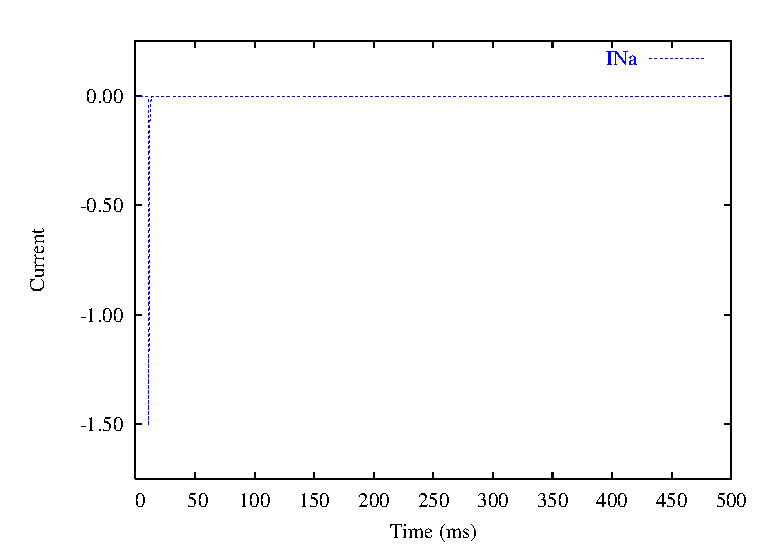
\includegraphics[width=\textwidth]{cardiac_electrophysiology/epsfiles/BR_INa.eps}
    \caption{}
  \end{subfigure}
  \hfill
  \begin{subfigure}[b]{0.45\linewidth}
    \centering
    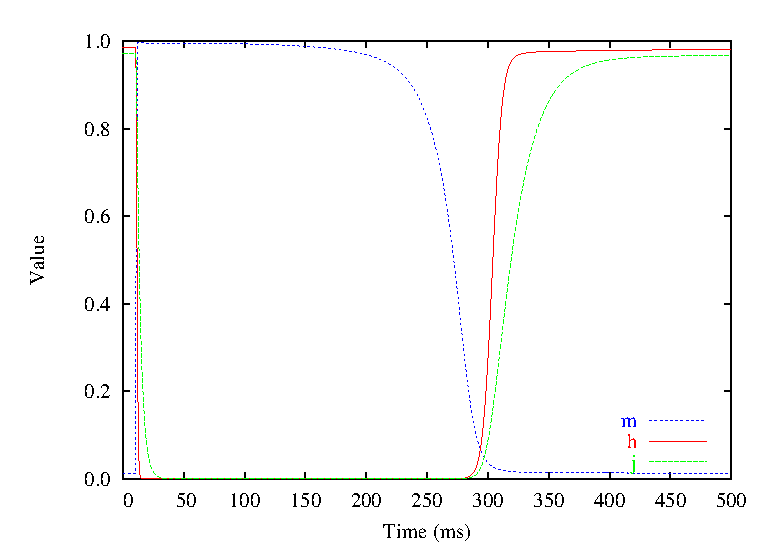
\includegraphics[width=\linewidth]{cardiac_electrophysiology/epsfiles/BR_mhj.eps} \\
    \caption{}
  \end{subfigure}
  \caption[Fast inward sodium current from the Beeler-Reuter model]{Figure(a) shows the
    fast inward sodium current over time and Figure(b) shows the $m$, $h$ and
    $j$ gate variables over time from the Beeler-Reuter model.}
  \label{fig:BR_NA_traces}
\end{figure}
%
\subsubsection{Time independent outward potassium current}
The magnitude of the time independent outward potassium current, $I_{K1}$ was
given by 
\begin{equation}
  I_{K1}=0.0035\sqbrac{\dfrac{4\pbrac{\exp\pbrac{0.04\pbrac{V_m+85}}-1}} 
    {\exp\pbrac{0.08\pbrac{V_m+53}}+\exp\pbrac{0.04\pbrac{Vm+53}}} 
    +\dfrac{0.2\pbrac{V_m+23}} {1-\exp\pbrac{-0.04\pbrac{V_m+23}}}} 
\end{equation}
and the temporal trace of the current is shown in \figref{fig:BR_ik1}.
\begin{figure}[hbtp] 
  \centering
  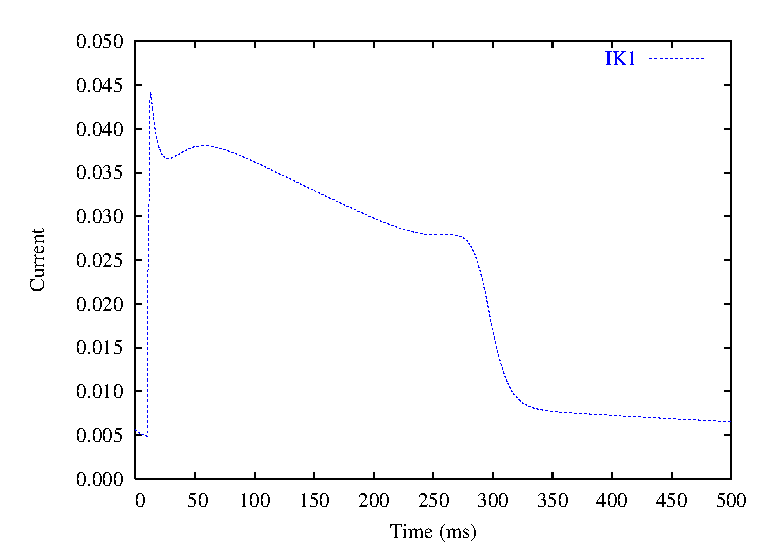
\includegraphics[width=75mm]{cardiac_electrophysiology/epsfiles/BR_IK1.eps}
  \caption[Beeler-Reuter time independent potassium current]{The time
    independent outward potassium current from the Beeler-Reuter model.}
  \label{fig:BR_ik1}
\end{figure}
%
\subsubsection{Time dependent outward potassium current}
The time dependent outward potassium current was controlled by a single
Hodgin-Huxley type gating variable, $x_1$.
\begin{equation}
  I_{x1}=8\times 10^{-3}\cdot x_1\cdot \sqbrac{\dfrac{\exp\pbrac{0.04\pbrac{V_m+77}}-1}
    {\exp\pbrac{0.04\pbrac{V_m+35}}}}
\end{equation}
where the time dependence of $x_1$ was defined to be 
\begin{equation}
  \dby{x_1}{t}=\alpha_{x1}\cdot\pbrac{1-x_1}-\beta_{x1}\cdot x_1
\end{equation}
The rate constants were calculated from
\begin{align}
  \alpha_{x1} =& 5\times 10^{-4}\sqbrac{\dfrac{\exp\pbrac{0.083\pbrac{V_m+50}}}
    {\exp\pbrac{0.057\pbrac{V_m+50}+1}}} \\
  \beta_{x1} =& 1.3\times 10^{-3}\sqbrac{\dfrac{\exp\pbrac{-0.06\pbrac{V_m+20}}}
    {\exp\pbrac{-0.04\pbrac{V_m+20}+1}}}
\end{align}
The size of the current and state of the gating variable over time are shown
in \figref{fig:BR_Ix1_traces}.
\begin{figure}[hbtp] 
  \centering
  \begin{subfigure}[b]{0.45\linewidth}
    \centering
    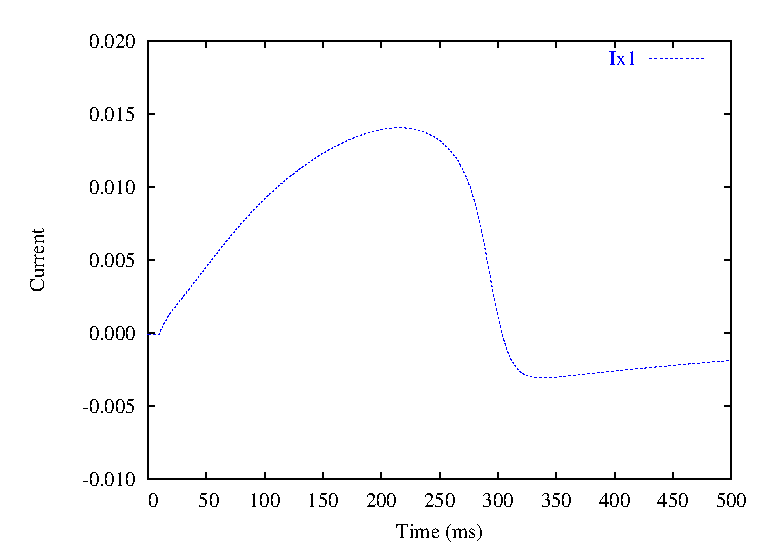
\includegraphics[width=\textwidth]{cardiac_electrophysiology/epsfiles/BR_Ix1.eps}
    \caption{}
  \end{subfigure}
  \hfill
  \begin{subfigure}[b]{0.45\linewidth}
    \centering
    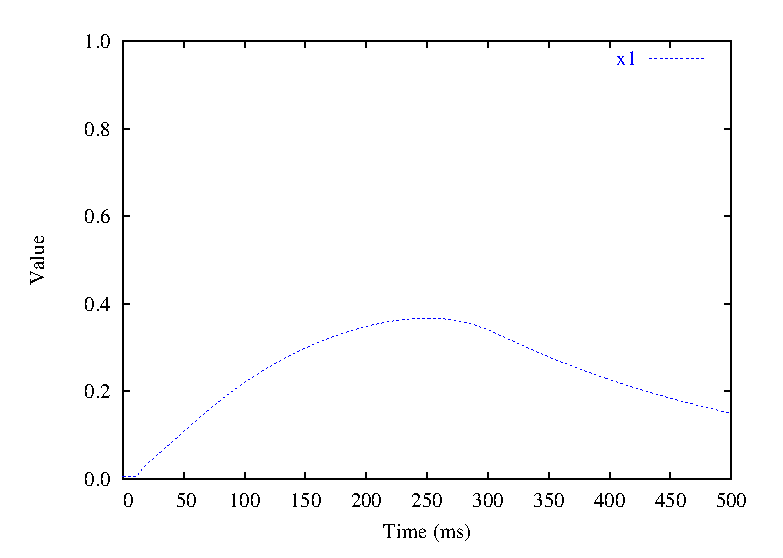
\includegraphics[width=\textwidth]{cardiac_electrophysiology/epsfiles/BR_x1.eps}
    \caption{}
  \end{subfigure}
  \caption[Beeler-Reuter time dependent potassium current]{Figure(a) shows the
    time dependent outward potassium current over time and Figure(b) shows the
    $x_1$ gate variable over time from the Beeler-Reuter model.}
  \label{fig:BR_Ix1_traces}
\end{figure}
%
\subsubsection{Slow inward current}
The slow inward current was based mainly around the uptake of calcium ions
into the cell. The current features an activation gate $d$ and an inactivation
gate $f$. The ionic current was represented by
\begin{equation}
  I_s=\overline{g_s}\cdot d\cdot f\cdot \pbrac{V_m-E_s}
\end{equation}
where $\overline{g_s}$ is the fully activated channel conductance which was
set to be $9\times 10^{-4}\mS\unitseparator\mm^{-2}$. The reversal potential
for the current was dependent on the concentration of calcium ions present in
the cell.
\begin{equation}
  E_s=-82.3-13.0287\fnof{ln}{0.001\conc{Ca^{2+}}{i}}
\end{equation}
The time dependence of the intracellular calcium concentration was governed by
\begin{equation}
  \dby{\conc{Ca^{2+}}{i}}{t}=-0.01 I_s + 0.07\pbrac{1\times 10^{-4} - \conc{Ca^{2+}}{i}}
\end{equation}
and the concentration is shown in \figref{fig:BR_cai}.
\begin{figure}[hbtp] 
  \centering
  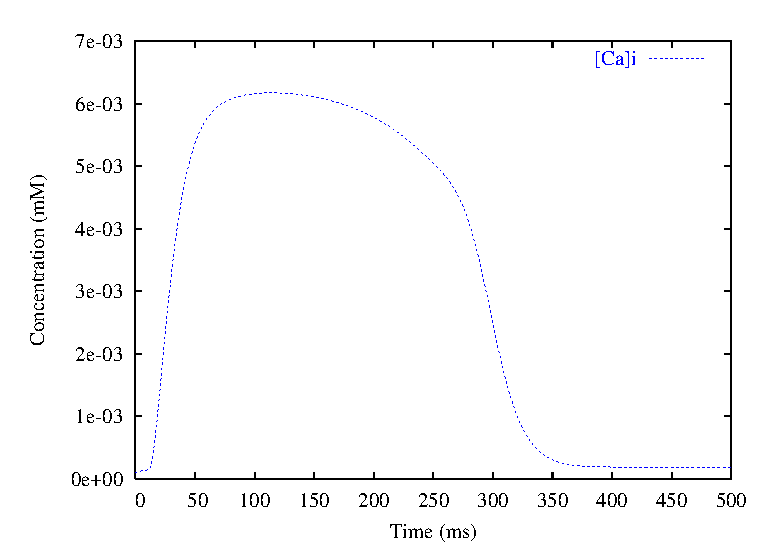
\includegraphics[width=75mm]{cardiac_electrophysiology/epsfiles/BR_Cai.eps}
  \caption[Beeler-Reuter intracellular calcium concentration]{The
    intracellular calcium ion concentration from the Beeler-Reuter model.}
  \label{fig:BR_cai}
\end{figure}
The two gating variables were calculated using
\begin{align}
  \label{eqn:br_dt}
  \dby{d}{t}=&\alpha_{d}\cdot\pbrac{1-d}-\beta_{d}\cdot d \\
  \label{eqn:br_ft}
  \dby{f}{t}=&\alpha_{f}\cdot\pbrac{1-f}-\beta_{f}\cdot f
\end{align}
The values of the rate constants were found from
\begin{align}
  \alpha_{d} =& 0.095\sqbrac{\dfrac{\exp\pbrac{-0.01\pbrac{V_m-5}}}
    {\exp\pbrac{-0.072\pbrac{V_m-5}}+1}} \\
  \beta_{d} =& 0.07\sqbrac{\dfrac{\exp\pbrac{-0.017\pbrac{V_m+44}}}
    {\exp\pbrac{0.05\pbrac{V_m+44}}+1}} \\
  \alpha_{f} =& 0.012\sqbrac{\dfrac{\exp\pbrac{-0.008\pbrac{V_m+28}}}
    {\exp\pbrac{0.15\pbrac{V_m+28}}+1}} \\
  \beta_{f} =& 0.0065\sqbrac{\dfrac{\exp\pbrac{-0.02\pbrac{V_m+30}}}
    {\exp\pbrac{-0.2\pbrac{V_m+30}}+1}}
\end{align}
The magnitude of the current and the state of the gating variables over time
is shown in \figref{fig:BR_Is_traces}.
\begin{figure}[hbtp] 
  \centering
  \begin{subfigure}[b]{0.45\linewidth}
    \centering
    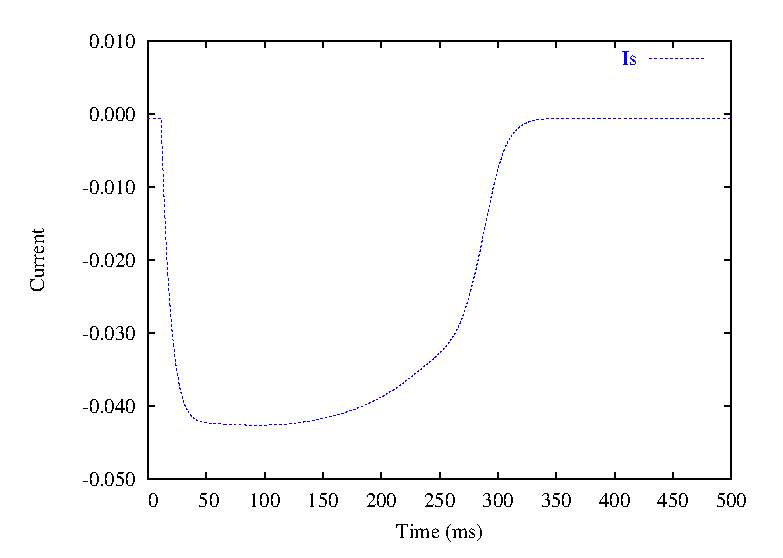
\includegraphics[width=\textwidth]{cardiac_electrophysiology/epsfiles/BR_Is.eps}
    \caption{}
  \end{subfigure}
  \hfill
  \begin{subfigure}[b]{0.45\linewidth}
    \centering
    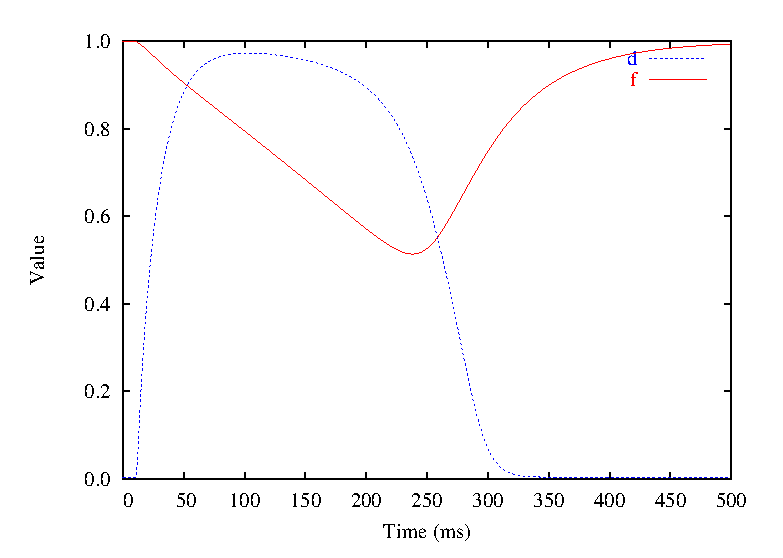
\includegraphics[width=\textwidth]{cardiac_electrophysiology/epsfiles/BR_df.eps}
    \caption{}
  \end{subfigure}
  \caption[Beeler-Reuter slow inward current]{Figure(a) shows the
    slow inward current over time and Figure(b) shows the
    $d$ and $f$ gate variables over time from the Beeler-Reuter model.}
  \label{fig:BR_Is_traces}
\end{figure}
%
The initial values of the gating variables were calculated from the initial
value of the transmembrane potential. The initial value for a gate $i$ was
given by
\begin{equation}
  i=\dfrac{\alpha_i}{\alpha_i+\beta_i}
\end{equation}
The values of the other parameters used in the Beeler-Reuter model whose
values have not yet been specified are given in \tabref{tab:BR_Model_Params}.
\begin{table}[hbtp] \centering
  \begin{tabular}{|c|c|c|}
    \hline
    \emph{Parameter} & \emph{Value} & \emph{Units}  \\ 
    \hline
    \hline 
    $V_m$  & $-84.0$ & $\mV$\\
    $\conc{Ca^{2+}}{i}$  & $1\times 10^{-4}$ & $\nM\unitseparator\mm^{-3}$\\
    $C_m$  & $0.01$ & $\uF\unitseparator\mm^{-2}$\\
    $A_m$ & $200$ & $\mm^{-1}$ \\
    \hline
  \end{tabular}
  \caption[Parameter values used in the Beeler-Reuter model]{Parameter values
    used in the Beeler-Reuter model}
  \label{tab:BR_Model_Params}
\end{table}
%
%===================================================================
\subsection{The defibrillation Beeler-Reuter model}
\label{sec:The_defibrillation_Beeler-Reuter_model}
%===================================================================
The original Beeler-Reuter model was modified by Drouhard and Roberge
to improve the fast sodium current kinetics. This model was then further
modified by \citet{skouibine:1999} to handle voltages outside the range of normal
physiological activity for use with defibrillation studies. The action
potential for the defibrillation Beeler-Reuter model is shown in
\figref{fig:BRDR_ap}.
\begin{figure}[hbtp] 
  \centering
  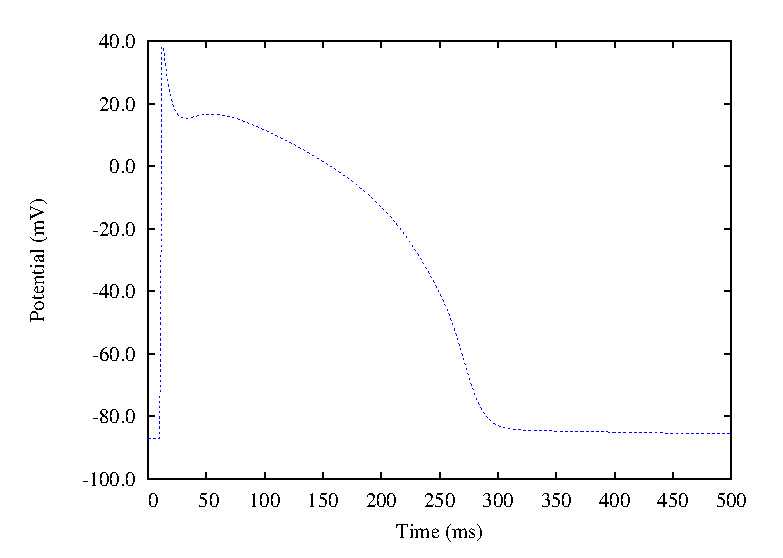
\includegraphics[width=75mm]{cardiac_electrophysiology/epsfiles/BRDR_Vm.eps}
  \caption[Defibrillation Beeler-Reuter action potential]{Action potential
    trace from the defibrillation Beeler-Reuter ionic current model.}
  \label{fig:BRDR_ap}
\end{figure}
%
\subsubsection{Fast inward sodium current}
The steady state sodium conductance, $\overline{g_{NaC}}$ was
removed along with the slow inactivation gating variable $j$ leaving the
following equation for the fast inward sodium current. 
\begin{equation}
  I_{Na}=\overline{g_{Na}}\cdot m^3\cdot h\cdot \pbrac{V_m-E_{Na}}
\end{equation}
where $E_{Na}$ was set to $40\mV$ which is smaller than the standard
Beeler-Reuter model and $\overline{g_{Na}}$ was set to $0.15\mS\unitseparator\mm^{-2}$,
nearly four times larger than in the original model. The gating variables were
altered to cope with the large potentials encountered during defibrillation.
\begin{gather}
  \label{eqn:brdr_ina_coeffs}
  \begin{aligned}
    \alpha_m &=
    \begin{cases}
      0.9\sqbrac{\dfrac{V_m+42.65}{1-\exp\pbrac{\pbrac{-0.22V_m-9.3830}}}}
        & \text{if $V_m \le 100\mV$} \\
      890.9437890\sqbrac{\dfrac{\exp\pbrac{\pbrac{0.0486479V_m-4.8647916}}}
        {1+5.93962526\exp\pbrac{\pbrac{0.0486479V_m-4.8647916}}}}
        & \text{if $V_m > 100\mV$} 
    \end{cases} \\
    \beta_m &=
    \begin{cases}
      1.437\exp\pbrac{\pbrac{-0.085V_m -3.37875}}
        & \text{if $V_m > -85\mV$} \\
      \dfrac{100}{1+\exp\pbrac{\pbrac{0.2597504V_m+22.0787804}}}
        & \text{if $V_m \le -85\mV$} 
    \end{cases} \\
    \alpha_h &=
    \begin{cases}
      0.1\exp\pbrac{\pbrac{-0.193V_m-15.37245}}
        & \text{if $V_m > -90\mV$} \\
      -12.0662845-0.1422598V_m
        & \text{if $V_m \le -90\mV$} 
    \end{cases} \\
    \beta_h &=
    \begin{cases}
      \dfrac{1.7}{1+\exp\pbrac{\pbrac{-0.095V_m-1.9475}}} 
        & \text{for all $V_m$}
    \end{cases}
  \end{aligned}
\end{gather}
The fast inward sodium current and the gating variables are shown in
\figref{fig:BRDR_NA_traces}.
\begin{figure}[hbtp] 
  \centering
  \begin{subfigure}[b]{0.45\linewidth}
    \centering
    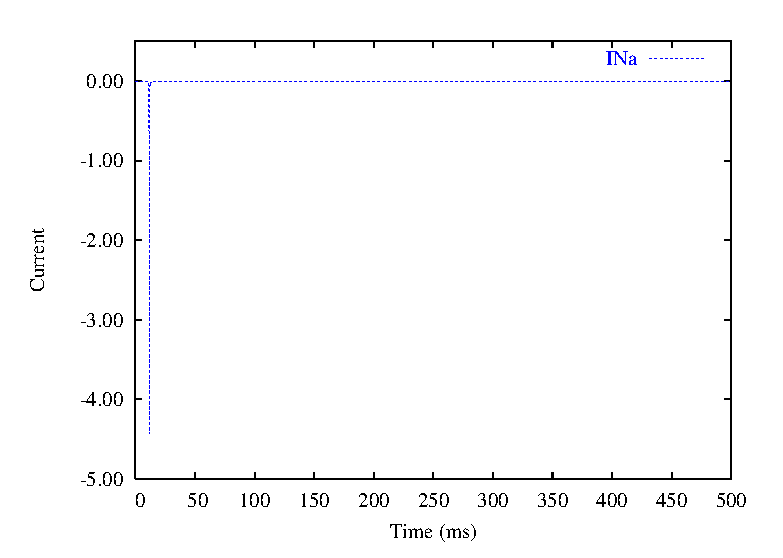
\includegraphics[width=\textwidth]{cardiac_electrophysiology/epsfiles/BRDR_INa.eps}
    \caption{}
  \end{subfigure}
  \hfill
  \begin{subfigure}[b]{0.45\linewidth}
    \centering
    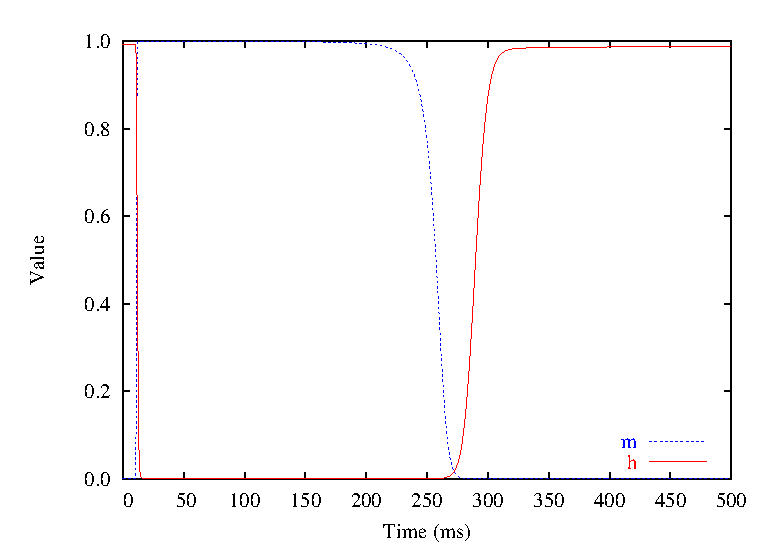
\includegraphics[width=\textwidth]{cardiac_electrophysiology/epsfiles/BRDR_mh.eps}
    \caption{}
  \end{subfigure}
  \caption[Fast inward sodium current from the defibrillation Beeler-Reuter
  model]{Figure(a) shows the 
    fast inward sodium current over time and Figure(b) shows the $m$, and $h$
    gating variables over time from the defibrillation Beeler-Reuter model.}
  \label{fig:BRDR_NA_traces}
\end{figure}
%
\subsubsection{Time independent outward potassium current}
The formula for time independent outward potassium current was unchanged. The
time course of the current is shown in \figref{fig:BRDR_ik1}
\begin{figure}[hbtp] 
  \centering
  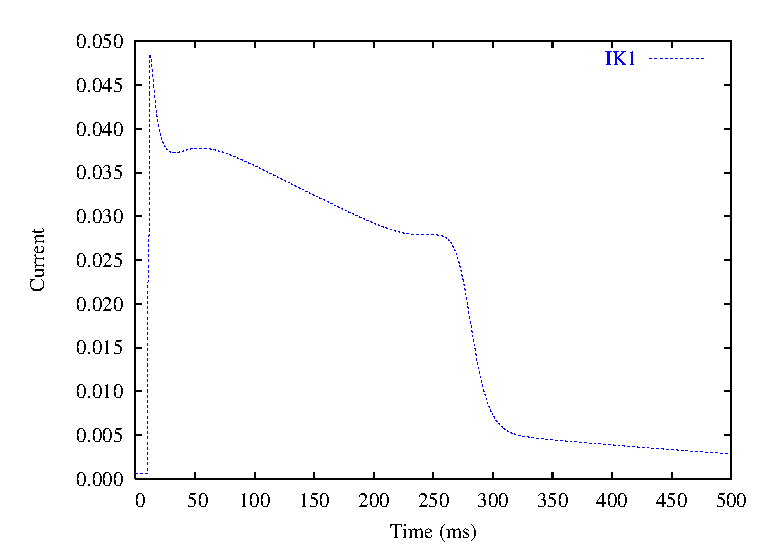
\includegraphics[width=75mm]{cardiac_electrophysiology/epsfiles/BRDR_IK1.eps}
  \caption[Defibrillation Beeler-Reuter time independent potassium current]{The time
    independent outward potassium current from the defibrillation Beeler-Reuter model.}
  \label{fig:BRDR_ik1}
\end{figure}
%
\subsubsection{Time dependent outward potassium current}
While the governing equations for the time dependent outward potassium current
were unchanged, the gating variables were modified to become
\begin{gather}
  \label{eqn:brdr_ix1_coeffs}
  \begin{aligned}
    \alpha_{x1} &=
    \begin{cases}
      0.0005\sqbrac{\dfrac{\exp\pbrac{\pbrac{0.083V_m+4.150}}}
        {\exp\pbrac{\pbrac{0.057V_m+2.850}}+1}}
        & \text{if $V_m \le 400\mV$} \\
      151.7994692\sqbrac{\dfrac{\exp\pbrac{\pbrac{0.0654679V_m-26.1871448}}}
        {1+1.5179947\exp\pbrac{\pbrac{0.0654679V_m-26.1871448}}}}
        & \text{if $V_m > 400\mV$} 
    \end{cases} \\
    \beta_{x1} &=
    \begin{cases}
      0.0013\sqbrac{\dfrac{\exp\pbrac{\pbrac{-0.06V_m-1.20}}}
      {\exp\pbrac{\pbrac{-0.04V_m-0.80}}+1}}
      & \text{for all $V_m$}
    \end{cases}
  \end{aligned}
\end{gather}
The size of the current and state of the gating variable over time are shown
in \figref{fig:BRDR_Ix1_traces}.
\begin{figure}[hbtp] 
  \centering
  \begin{subfigure}[b]{0.45\linewidth}
    \centering
    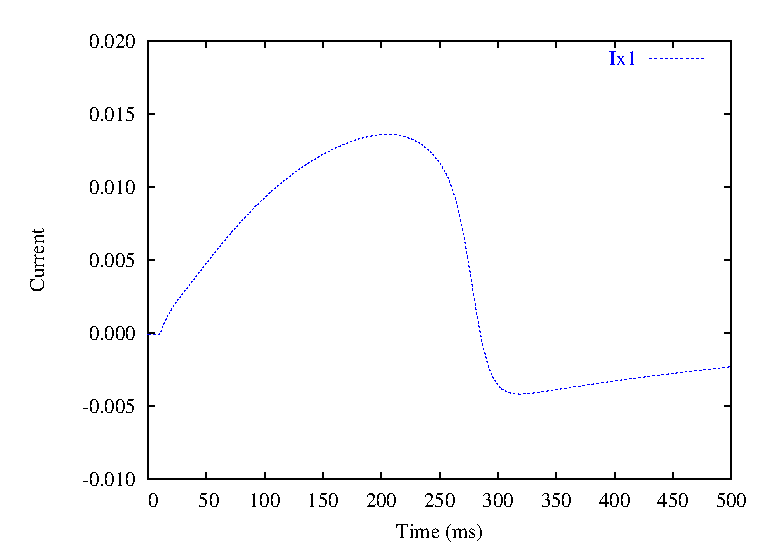
\includegraphics[width=\textwidth]{cardiac_electrophysiology/epsfiles/BRDR_Ix1.eps}
    \caption{}
  \end{subfigure}
  \hfill
  \begin{subfigure}[b]{0.45\linewidth}
    \centering
    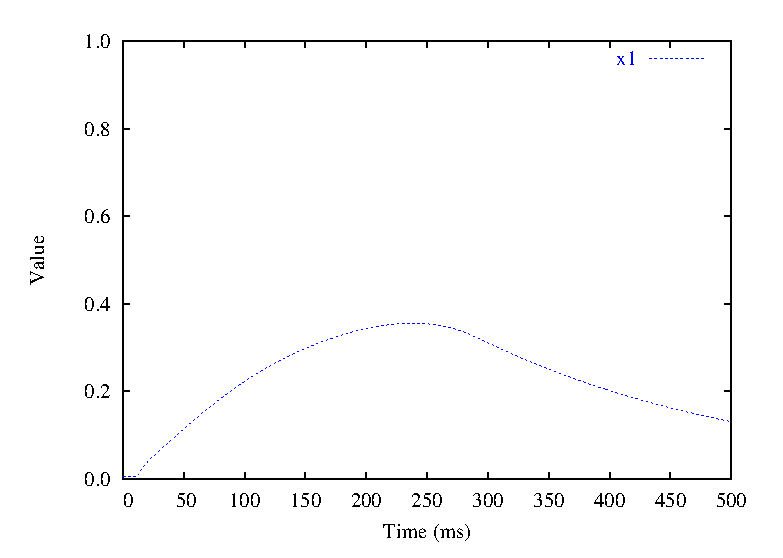
\includegraphics[width=\textwidth]{cardiac_electrophysiology/epsfiles/BRDR_x1.eps}
    \caption{}
  \end{subfigure}
  \caption[Defibrillation Beeler-Reuter time dependent potassium current]{Figure(a) shows the
    time dependent outward potassium current over time and Figure(b) shows the
    $x_1$ gate variable over time from the defibrillation Beeler-Reuter model.}
  \label{fig:BRDR_Ix1_traces}
\end{figure}
%
\subsubsection{Slow inward current}
There was a change made to the intracellular calcium ion tracking in order to
limit the movement of calcium ions at large potentials.
\begin{gather}
  \label{eqn:two_cases_of_caiBRDR}
  \begin{aligned}
    \dby{\conc{Ca^{2+}}{i}}{t} &=
    \begin{cases}
      -0.01 I_s + 0.07\pbrac{1\times 10^{-4} - \conc{Ca^{2+}}{i}}
        & \text{if $V_m \le 200\mV$} \\
      0
        & \text{if $V_m > 200\mV$} 
    \end{cases}
  \end{aligned}
\end{gather}
The time course of the intracellular calcium ion concentration is shown in
\figref{fig:BRDR_cai}. 
\begin{figure}[hbtp] 
  \centering
  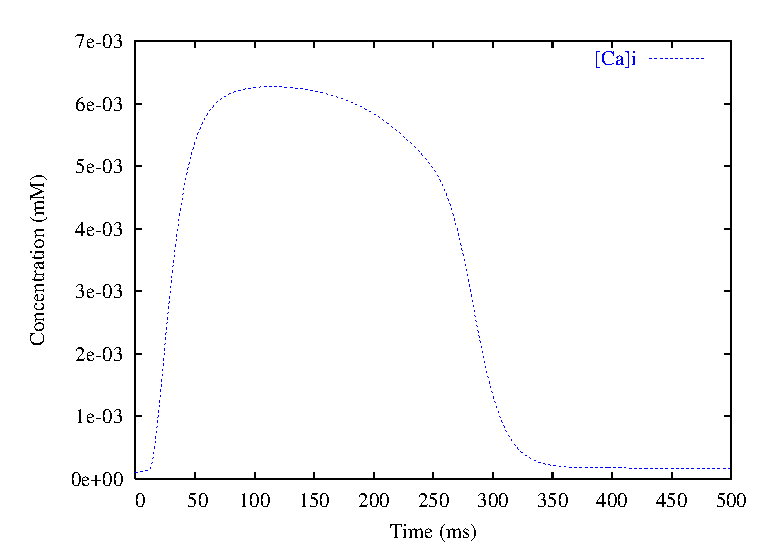
\includegraphics[width=75mm]{cardiac_electrophysiology/epsfiles/BRDR_Cai.eps}
  \caption[Defibrillation Beeler-Reuter intracellular calcium concentration]{The
    intracellular calcium ion concentration from the defibrillation Beeler-Reuter model.}
  \label{fig:BRDR_cai}
\end{figure}

In addition to these changes, in order to simulate ischemic tissue a scale
factor was added to the time dependent $d$ and $f$ gates to allow the scaling
of the action potential duration. The
modified equations became
\begin{align}
  \dby{d}{t}=&\dfrac{\alpha_{d}}{R}\cdot \pbrac{1-d}-\beta_{d}\cdot  d \\
  \dby{f}{t}=&\dfrac{\alpha_{f}}{R}\cdot \pbrac{1-f}-\beta_{f}\cdot  f
\end{align}
where $R$ was typically in the range of $1$ to $8$. 
The slow inward current and associated gating variables are shown in
\figref{fig:BRDR_Is_traces}.
\begin{figure}[hbtp] 
  \centering
  \begin{subfigure}[b]{0.45\linewidth}
    \centering
    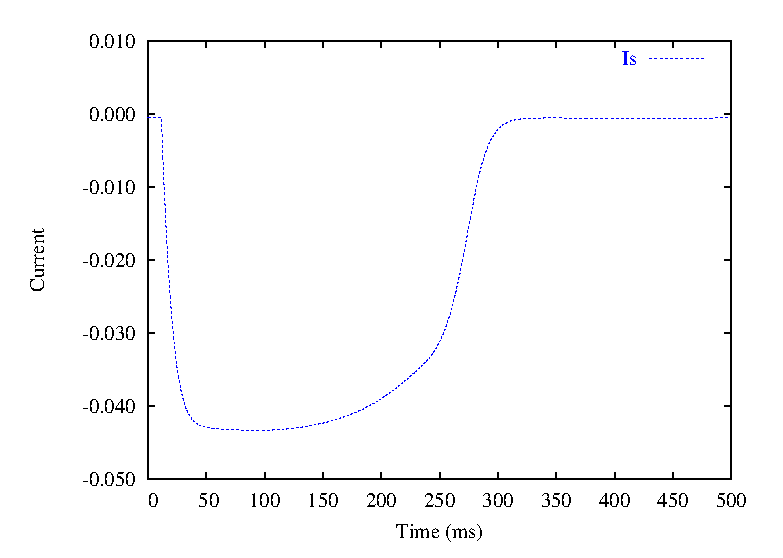
\includegraphics[width=\textwidth]{cardiac_electrophysiology/epsfiles/BRDR_Is.eps}
    \caption{}
  \end{subfigure}
  \hfill
  \begin{subfigure}[b]{0.45\linewidth}
    \centering
    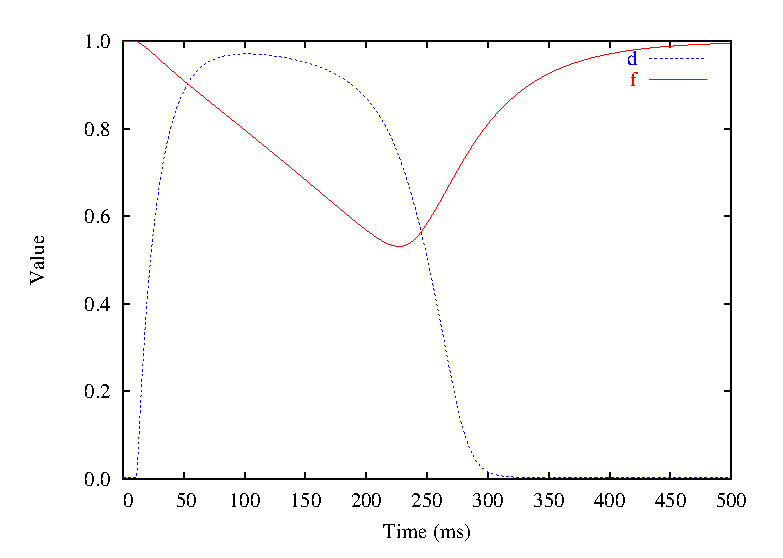
\includegraphics[width=\textwidth]{cardiac_electrophysiology/epsfiles/BRDR_df.eps}
    \caption{}
  \end{subfigure}
  \caption[Defibrillation Beeler-Reuter slow inward current]{Figure(a) shows the
    slow inward current over time and Figure(b) shows the
    $d$ and $f$ gate variables over time from the defibrillation Beeler-Reuter model.}
  \label{fig:BRDR_Is_traces}
\end{figure}
%
%===================================================================
\subsection{The Luo-Rudy models}
\label{sec:The_Luo-Rudy_I_model}
%===================================================================
The Luo-Rudy model \cite{luo:1991} built on the Beeler-Reuter model adjusting the
parameters to more recent experimental results and adding more currents to
more accurately represent the potassium ion dynamics. Six individual currents
were used to describe the cellular processes.
\begin{equation}
  I_{ion}=I_{Na}+I_{si}+I_{K}+I_{K1}+I_{Kp}+I_{b}
\end{equation}
Three of the currents may be grouped to give an expression for the total time
independent potassium current.
\begin{equation}
  I_{K1T}=I_{K1}+I_{Kp}+I_{b}
\end{equation}
A plot of $I_{K1T}$ is shown later in \figref{fig:LR_IbK1T_traces}. In
addition to these ionic currents the intracellular calcium ion
concentration was tracked due to the calcium uptake by the slow inward
current, $I_{si}$. The action potential produced by the Luo-Rudy model is
shown in \figref{fig:LR1_ap}.
\begin{figure}[hbtp] 
  \centering
  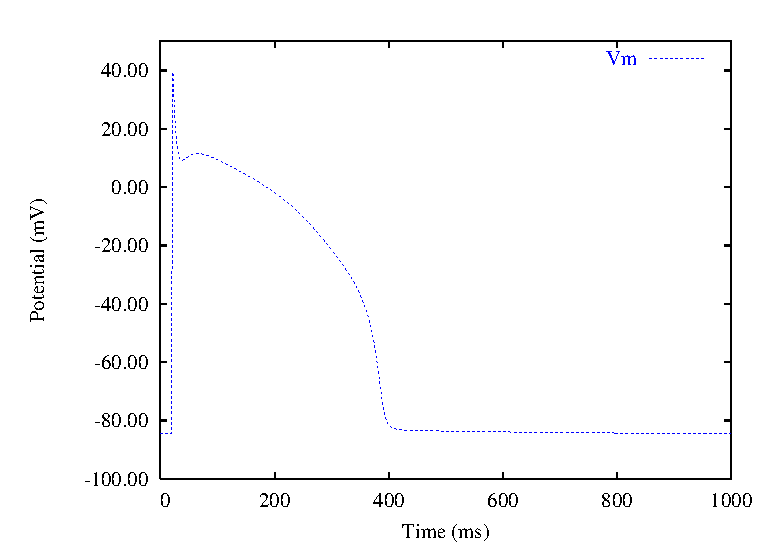
\includegraphics[width=75mm]{cardiac_electrophysiology/epsfiles/LR_Vm.eps}
  \caption[Luo-Rudy action potential]{Action potential trace from the Luo-Rudy
    ionic current model.}
  \label{fig:LR1_ap}
\end{figure}
%
\subsubsection{Fast inward sodium current}
The general form of the fast inward sodium current is the same as the original
Beeler-Reuter model with the omission of the steady state sodium conductance
parameter.
\begin{equation}
  I_{Na}=\overline{g_{Na}}\cdot m^3\cdot h\cdot j\cdot\pbrac{V_m-E_{Na}}
\end{equation}
Here $m$ is the activation gate, $h$ is the fast inactivation gate and $j$ is the slow
inactivation gate. The time dependent behaviour of these gates was identical to the
Beeler-Reuter model \eqnthrurefs{eqn:br_mt}{eqn:br_jt} but with reformulated
rate constants. $\overline{g_{Na}}$ is
the maximum sodium conductance and $E_{Na}$ is the reversal potential of the
channel as calculated from the Nernst potential for sodium ions using
\eqnref{eqn:lr1reversal}. The $\alpha$ and $\beta$ gating parameters were
defined to be
\begin{gather}
  \label{eqn:lr1_ina_coeffs}
  \begin{aligned}
    \alpha_m &= {0.32  (V_m+47.13) \over 1-\exp(-0.1(V_m+47.13))} \\
    \beta_m &= 0.08  \exp(-V_m / 11) \\
    \alpha_h &=
    \begin{cases}
      0 & \text{if $V_m \geq -40 \mV$} \\
      0.135  \exp[(-80.0-V_m) / 6.8] & \text{if $V_m < -40 \mV$}
    \end{cases} \\
    \beta_h &=
    \begin{cases}
      \frac{1}{0.13  (1 + \exp[- (V_m+10.66) / 11.1])} &
      \text{if $V_m \geq -40 \mV$} \\
      3.56  \exp(0.079 V_m) + \nttento{3.1}{5}  \exp(0.35  V_m) & 
      \text{if $V_m < -40 \mV$}
    \end{cases} \\
    \alpha_j &= 
    \begin{cases}
      0 & \text{if $V_m \geq -40 \mV$} \\
      \frac{\nttento{-1.2714}{5} \exp(0.2444 V_m) - \nttento{3.474}{-5} 
      \exp(-0.04391 V_m)}{1+\exp\left(0.311 (V_m+79.23) \right)} (V_m+37.78)&
      \text{if $V_m < -40 \mV$}
    \end{cases} \\
    \beta_j &=
    \begin{cases}
      0.3  \exp(\nttento{-2.535}{-7}  V_m) \over \left(1+\exp\left(-0.1 
          (V_m+32) \right) \right) & \text{if $V_m \geq -40 \mV$} \\
      0.1212  \exp( -0.01052  V_m) \over \left(1+\exp\left(-0.1378 
          (V_m+40.14) \right) \right)
      & \text{if $V_m < -40 \mV$}
    \end{cases}
  \end{aligned}
\end{gather}
The fast inward sodium current and the three gating variables are shown in
\figref{fig:LR_NA_traces}.
\begin{figure}[hbtp] 
  \centering
  \begin{subfigure}[b]{0.45\linewidth}
    \centering
    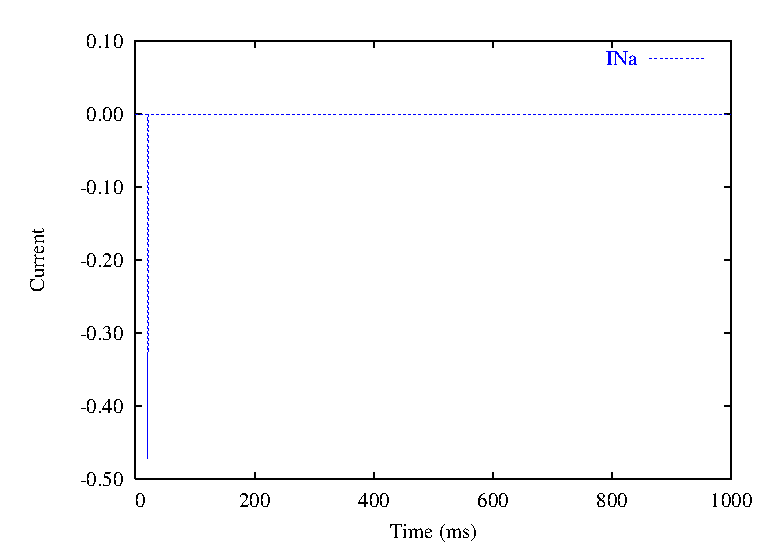
\includegraphics[width=\textwidth]{cardiac_electrophysiology/epsfiles/LR_INa.eps}
    \caption{}
  \end{subfigure}
  \hfill
  \begin{subfigure}[b]{0.45\linewidth}
    \centering
    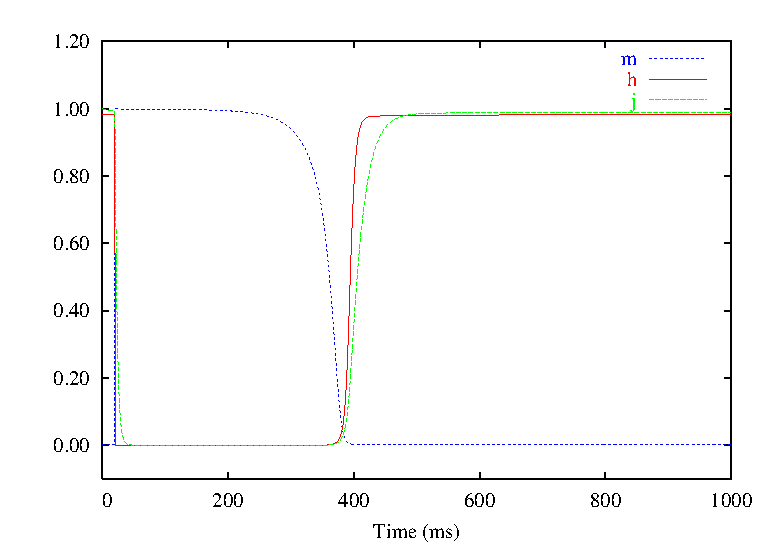
\includegraphics[width=\textwidth]{cardiac_electrophysiology/epsfiles/LR_NaGates.eps}
    \caption{}
  \end{subfigure}
  \caption[Fast inward sodium current from the Luo-Rudy model]{Figure(a) shows the
    fast inward sodium current over time and Figure(b) shows the $m$, $h$ and
    $j$ gate variables over time from the Luo-Rudy model.}
  \label{fig:LR_NA_traces}
\end{figure}
%
\subsubsection{Slow inward current}
The slow inward current was defined by the same formula as the $I_s$ current
in the Beeler Reuter model.
\begin{equation}
  I_{si}=\overline{g_{si}}\cdot d\cdot f\cdot \pbrac{V_m-E_{si}}
\end{equation}
The reversal potential was adjusted to be
\begin{equation}
  E_{si}=7.7-13.0287\ln\pbrac{\conc{Ca^{2+}}{i}}
\end{equation}
and the formulation of the rate constants, $\alpha_d$,$\beta_d$,$\alpha_f$
and $\beta_f$ were also unchanged. The current trace over time along with the
two gates are shown in \figref{fig:LR_Isi_traces}.
\begin{figure}[hbtp] 
  \centering
  \begin{subfigure}[b]{0.45\linewidth}
    \centering
    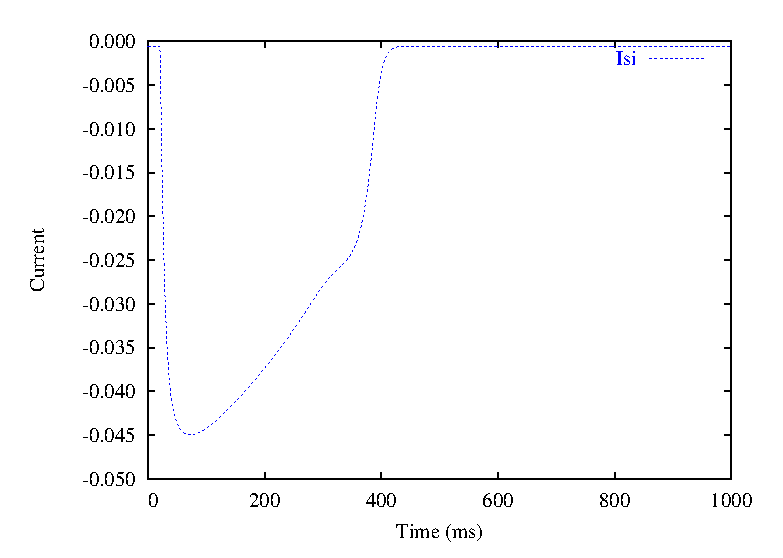
\includegraphics[width=\textwidth]{cardiac_electrophysiology/epsfiles/LR_Isi.eps}
    \caption{}
  \end{subfigure}
  \hfill
  \begin{subfigure}[b]{0.45\linewidth}
    \centering
    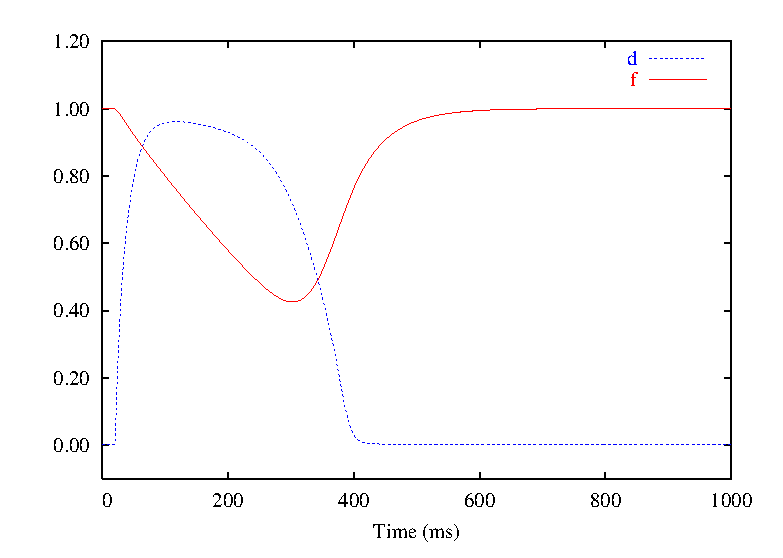
\includegraphics[width=\textwidth]{cardiac_electrophysiology/epsfiles/LR_SIGates.eps}
    \caption{}
  \end{subfigure}
  \caption[Slow inward current from the Luo-Rudy model]{Figure(a) shows the
    slow inward current over time and Figure(b) shows the $d$ and
    $f$ gate variables over time from the Luo-Rudy model.}
  \label{fig:LR_Isi_traces}
\end{figure}
%
\subsubsection{Time dependent potassium current}
The time dependent potassium current was controlled by an activation gate, $x$
and an inactivation gate, $X_i$. The inactivation gate was not formulated as a
typical Hodgkin-Huxley differential equation. 
\begin{equation}
  I_K=\overline{g_{K}}\cdot x\cdot X_i\cdot \pbrac{V_m-E_{K}}
\end{equation}
where the maximum potassium conductance was calculated from
\begin{equation}
  \overline{g_{K}}=g_{K}\cdot \sqrt{\conc{K^+}{o}/5.4}
\end{equation}
The reversal potential was calculated from
\begin{equation}
  E_K=\dfrac{RT}{F}\ln\pbrac{\dfrac{\conc{K^+}{o}+PR_{NaK}
      \conc{Na^+}{o}}{\conc{K^+}{i}+PR_{NaK}\conc{Na^+}{i}}}
\end{equation}
where $PR_{NaK}$ is a dimensionless permeability ratio. The rate constants
for the $x$ gate were 
defined to be the same as in the Beeler-Reuter model where the gate is
referenced as the $x1$ gate. This model introduces a new inactivation gate,
$X_i$, which was given by
\begin{gather}
  \begin{aligned}
    X_i &=
    \begin{cases}
      1.0 & \text{if $V_m \leq -100 \mV$} \\
      2.837 \dfrac{\exp\pbrac{0.04\pbrac{V_m+77}}-1}{\pbrac{V_m+77}
        \exp\pbrac{0.04\pbrac{V_m+35}}} & \text{otherwise}
    \end{cases} \\ 
  \end{aligned}
\end{gather}
The temporal trace of the time dependent potassium current along with the $x$
gating variable is shown in \figref{fig:LR_IK_traces}.
\begin{figure}[hbtp] 
  \centering
  \begin{subfigure}[b]{0.45\linewidth}
    \centering
    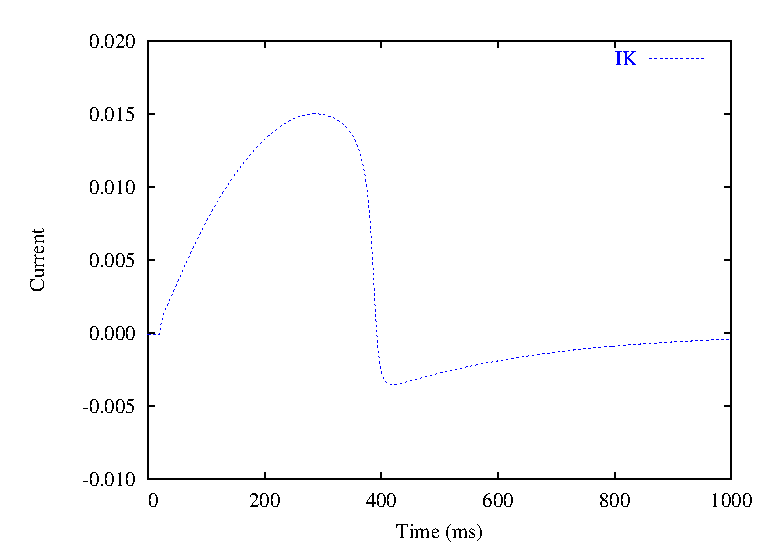
\includegraphics[width=\textwidth]{cardiac_electrophysiology/epsfiles/LR_IK.eps}
    \caption{}
  \end{subfigure}
  \hfill
  \begin{subfigure}[b]{0.45\linewidth}
    \centering
    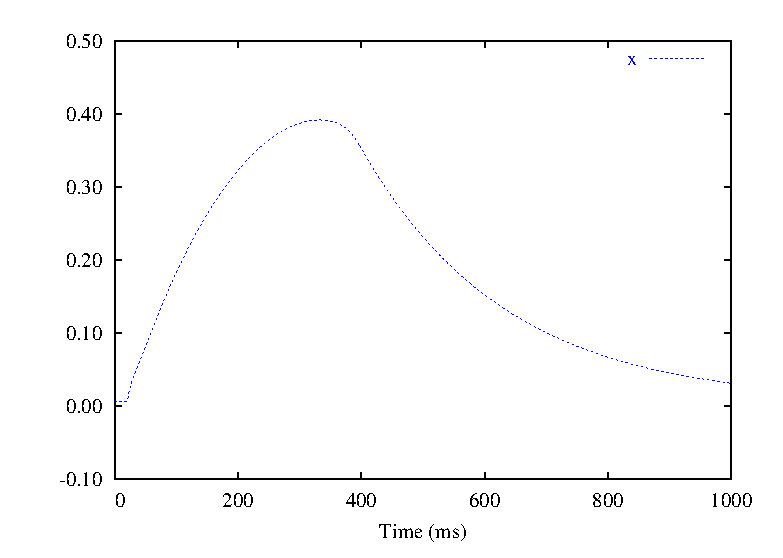
\includegraphics[width=\textwidth]{cardiac_electrophysiology/epsfiles/LR_Xgate.eps}
    \caption{}
  \end{subfigure}
  \caption[Time dependent outward current from the Luo-Rudy model]{Figure(a) shows the
    time dependent outward current over time and Figure(b) shows the $x$ gate
    over time from the Luo-Rudy model.}
  \label{fig:LR_IK_traces}
\end{figure}
%
\subsubsection{Time independent potassium current}
While present in the Beeler-Reuter model the time independent potassium
current has been formulated differently along with the addition of two further
potassium based time independent currents, $I_{Kp}$ and $I_b$. This model uses
one gating variable with a time constant small enough that it may be
approximated by a steady state formulation.
\begin{equation}
  I_{K1}=\overline{g_{K1}}\cdot K_{1\infty}\cdot \pbrac{V_m-E_{K1}}
\end{equation}
The reversal potential was the Nernst potential for potassium ions found from
\eqnref{eqn:lr1reversal}. The maximum channel conductance was calculated by
\begin{equation}
  \overline{g_{K1}}=g_{K1}\cdot \sqrt{\conc{K^+}{o}/5.4}
\end{equation}
The steady gating parameter, $K_{1\infty}$ was calculated to be
\begin{equation}
  K_{1\infty}=\dfrac{\alpha_{K1}}{\alpha_{K1}+\beta{K1}}
\end{equation}
where the rate constants were given by
\begin{align}
  \alpha_{K1}=& \dfrac{1.02}{1+\exp\sqbrac{0.2385\pbrac{V_m-E_{K1}-59.215}}} \\
  \beta_{K1}=& \dfrac{{0.49124\exp\sqbrac{0.08032\pbrac{V_m-E_{K1}+5.476}}}+
    {\exp\sqbrac{0.06175\pbrac{V_m-E_{K1}-594.31}}}}{1+\exp\sqbrac{-0.5143
    \pbrac{V_m-E_{K1}+4.753}}}
\end{align}
A plot of the time independent potassium current is shown in \figref{fig:LR_IK1p_traces}.
%
\subsubsection{Plateau potassium current}
The reversal potential for the plateau potassium current was the same as the
reversal potential of the time independent potassium current.
\begin{equation}
  E_{Kp}=E_{K1}
\end{equation}
The ionic current was given by
\begin{equation}
 I_{Kp}=\overline{g_{Kp}}\cdot K_p\cdot \pbrac{V_m-E_{Kp}}
\end{equation}
where
\begin{equation}
  K_p=\dfrac{1}{1+\exp\pbrac{\pbrac{7.488-V_m}/5.98}}
\end{equation}
A plot of the plateau potassium current is shown in \figref{fig:LR_IK1p_traces}.
\begin{figure}[hbtp] 
  \centering
  \begin{subfigure}[b]{0.45\linewidth}
    \centering
    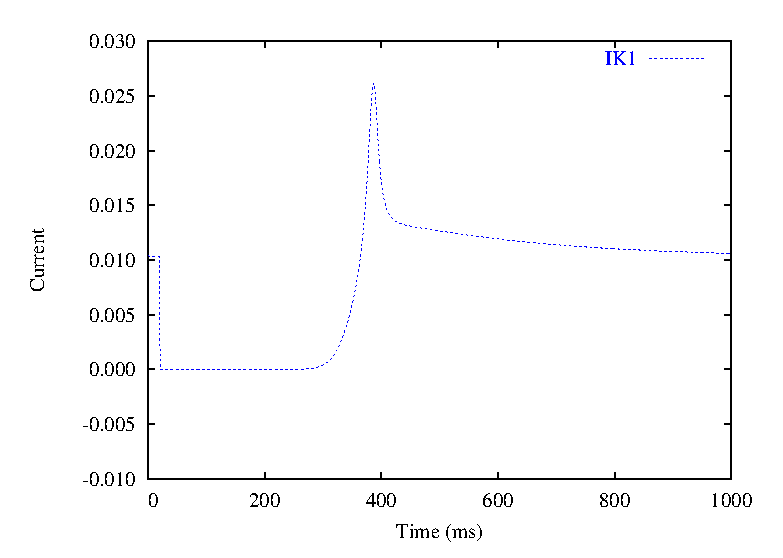
\includegraphics[width=\textwidth]{cardiac_electrophysiology/epsfiles/LR_IK1.eps}
    \caption{}
  \end{subfigure}
  \hfill
  \begin{subfigure}[b]{0.45\linewidth}
    \centering
    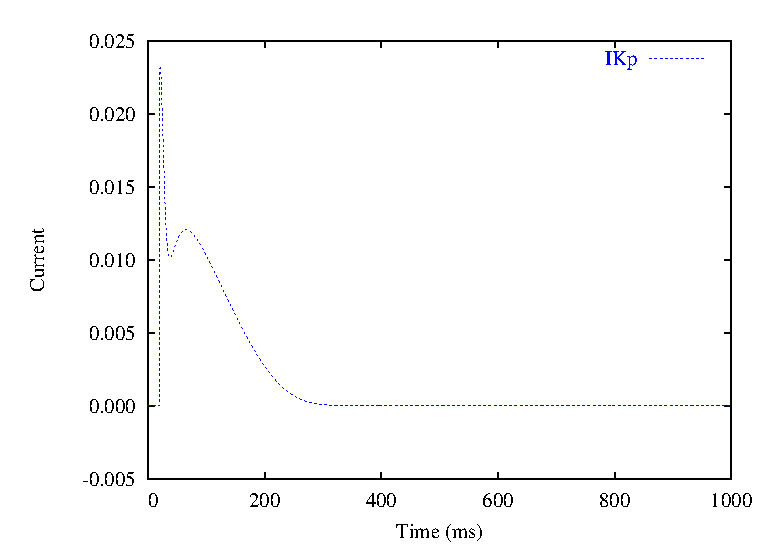
\includegraphics[width=\textwidth]{cardiac_electrophysiology/epsfiles/LR_IKp.eps}
    \caption{}
  \end{subfigure}
  \caption[Time independent and plateau currents from the Luo-Rudy model]{Figure(a) shows the
    time independent outward current over time and Figure(b) shows the plateau
    current over timefrom the Luo-Rudy model.}
  \label{fig:LR_IK1p_traces}
\end{figure}
%
\subsubsection{Background current}
The background current was given by
\begin{equation}
  I_b=\overline{g_{b}}\cdot \pbrac{V_m+59.87}
\end{equation}
and a plot of the background current over time is shown in \figref{fig:LR_IbK1T_traces}.
\begin{figure}[hbtp] 
  \centering
  \begin{subfigure}[b]{0.45\linewidth}
    \centering
    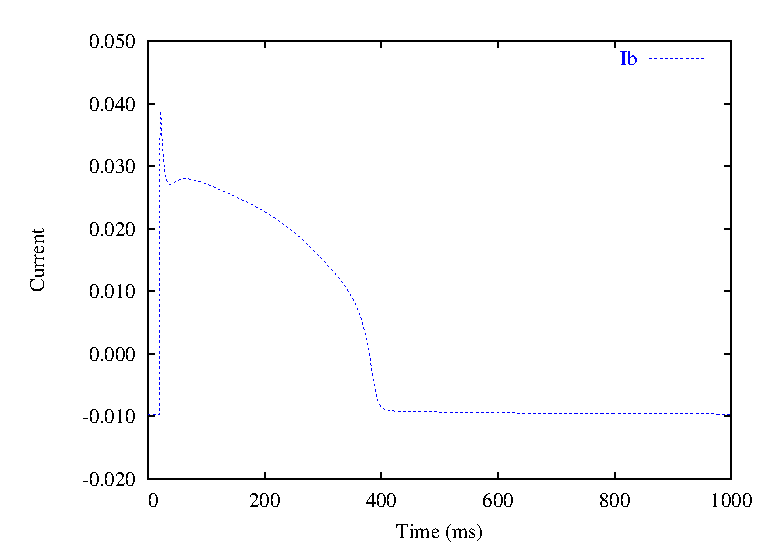
\includegraphics[width=\textwidth]{cardiac_electrophysiology/epsfiles/LR_Ib.eps}
    \caption{}
  \end{subfigure}
  \hfill
  \begin{subfigure}[b]{0.45\linewidth}
    \centering
    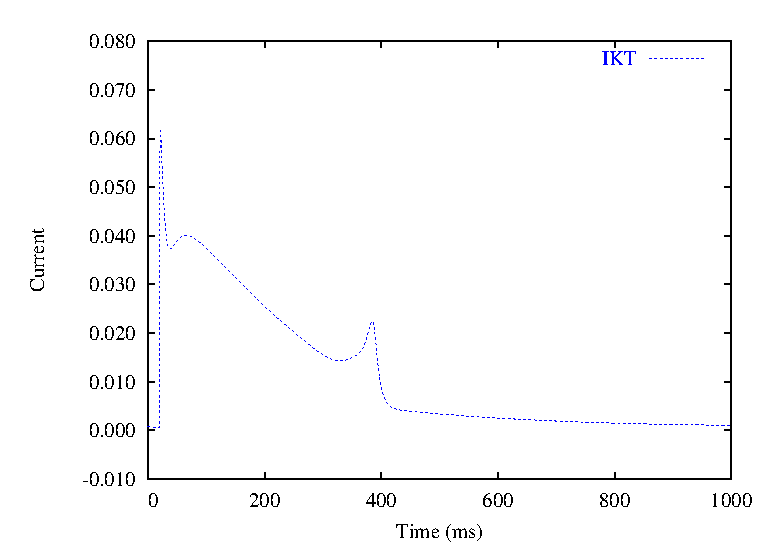
\includegraphics[width=\textwidth]{cardiac_electrophysiology/epsfiles/LR_IKT.eps}
    \caption{}
  \end{subfigure}
  \caption[Background and total time independent currents from the Luo-Rudy
  model]{Figure(a) shows the 
    background current over time and Figure(b) shows the total time
    independent potassium current over time from the Luo-Rudy model.}
  \label{fig:LR_IbK1T_traces}
\end{figure}
%
\subsubsection{Model parameters}
The set of model parameters in consistent units used with the Luo-Rudy model
are given in this section. The initial value of the transmembrane potential
was set to be $-84.5\mV$. The initial values of the gating variables which
were also time dependent are shown in \tabref{tab:lr1_init_gates}.
\begin{table}[hbtp] \centering
  \begin{tabular}{|c|c|}
    \hline
    \emph{Gate} & \emph{Initial value} \\ 
    \hline
    \hline 
      $m$ & $1.67 \times 10^{-3}$ \\
      $h$ & $9.38 \times 10^{-1}$ \\
      $j$ & $1.0$ \\
      $d$ & $2.98 \times 10^{-3}$ \\
      $f$ & $1.0$ \\
      $x$ & $6.02 \times 10^{-3}$ \\
    \hline
  \end{tabular}
  \caption[Initial gate values for the Luo-Rudy I model]{Initial gate
    values for the Luo-Rudy I model}
  \label{tab:lr1_init_gates}
\end{table}
The other time dependent quantity is the intracellular calcium
concentration. All of the other concentrations were constant over time. 
The intracellular and extracellular ion concentrations for the three
ions included in the model are shown in \tabref{tab:lr1_init_ions}.
\begin{table}[hbtp] \centering
  \begin{tabular}{|c|c|}
    \hline
    \emph{Ion} & \emph{Initial value} \\ 
    \hline
    \hline 
      $\conc{Ca^{2+}}{i}$ & $1.78 \times 10^{-4}$ \\
      $\conc{Ca^{2+}}{o}$ & $1.8$ \\
      $\conc{K^{+}}{i}$ & $1.45 \times 10^{2}$ \\
      $\conc{K^{+}}{o}$ & $5.4$ \\
      $\conc{Na^{+}}{i}$ & $1.8 \times 10^{1}$ \\
      $\conc{Na^{+}}{o}$ & $1.4 \times 10^{2}$ \\
    \hline
  \end{tabular}
  \caption[Initial ion concentrations for the Luo-Rudy I model]{Initial ion
    concentrations for the Luo-Rudy I model}
  \label{tab:lr1_init_ions}
\end{table}
All concentrations are given in $\nM\unitseparator\mm^{-3}=\mM$. Where in the
Beeler-Reuter model the reversal potentials of a given channel were
directly set, in this model they were calculated from the ion concentrations. The
reversal potential of a particular ion $x$ was defined by its Nernst potential to be 
\begin{equation}
  E_{x}=\pbrac{\dfrac{RT}{z_xF}}\ln{\dfrac{\conc{x}{o}}{\conc{x}{i}}}
  \label{eqn:lr1reversal}
\end{equation}
where $R$ is the gas constant, $T$ is temperature, $F$ is Faradays constant
$z_x$ is the valence of ion $x$ and $\conc{x}{o}$,$\conc{x}{i}$ were the
extracellular and intracellular 
concentrations of ion $x$ respectively. The maximum conductance values used
are shown in \tabref{tab:lr1_conductance}.  
\begin{table}[hbtp] \centering
  \begin{tabular}{|c|c|}
    \hline
    \emph{Parameter} & \emph{Value} \\ 
    \hline
    \hline 
      $\overline{g_{Na}}$ & $2.3 \times 10^{-1}$ \\
      $\overline{g_{si}}$ & $9.0 \times 10^{-4}$ \\
      $g_{K}$ & $2.82 \times 10^{-3}$ \\
      $g_{K1}$ & $6.047 \times 10^{-3}$ \\
      $\overline{g_{Kp}}$ & $1.83 \times 10^{-4}$ \\
      $\overline{g_{b}}$ & $3.921 \times 10^{-4}$ \\
    \hline
  \end{tabular}
  \caption[Conductance values for the Luo-Rudy I model]{Conductance
    values for the Luo-Rudy I model}
  \label{tab:lr1_conductance}
\end{table}
All conductances are given in $\mS\unitseparator\mm^{-2}$. It should be noted
that the maximum conductances for $g_{K}$ and $g_{K1}$ are calculated
elsewhere in the model using these values. The values for the other parameters
used in the model are shown in \tabref{tab:lr1_params}. Here $C_m$ is the
membrane capacitance and $A_m$ is the surface to volume 
ratio. 
\begin{table}[hbtp] \centering
  \begin{tabular}{|c|c|c|}
    \hline
    \emph{Parameter} & \emph{Value} & \emph{Units}\\ 
    \hline
    \hline 
      $C_m$ & $1.0 \times 10^{-2}$ & $\uF\unitseparator\mm^{-2}$ \\
      $A_m$ & $1.0 \times 10^{2}$  & $\pmm$ \\
      $R$ & $8.314472 \times 10^{3}$ & $\pJ\unitseparator
      \nM^{-1}\unitseparator \degK^{-1}$ \\
      $T$ & $3.1 \times 10^{2}$ & $\degK$\\
      $F$ & $9.648534 \times 10^{4}$ & $\nC\unitseparator\nM^{-1}$ \\
      $PR_{NaK}$ & $1.833 \times 10^{-2}$ & $dimensionless$ \\
    \hline
  \end{tabular}
  \caption[Parameter values for the Luo-Rudy I model]{Parameter
    values for the Luo-Rudy I model}
  \label{tab:lr1_params}
\end{table}
%
%===================================================================
%\subsection{The Luo-Rudy II model}
%\label{sec:The_Luo-Rudy_II_model}
%===================================================================
\subsubsection{The Luo-Rudy II model}
The second model published by Luo and Rudy \cite{luo:1994a} has become a widely used
model in the field of cellular cardiac activation and while designed
for mammalian ventricular cells was based mainly on the guinea pig. Again the
units of the model parameters where adjusted to retain unit consistency. One
of the main features of the model was the inclusion of more detailed calcium
dynamics. The model used $15$ ionic currents to generate action potentials.
\begin{align}
  I_{ion} =&
  I_{Na}+I_{Ca\pbrac{L}}+I_{K}+I_{K1}+I_{Kp}+I_{NaCa}+I_{NaK}+I_{ns\pbrac{Ca}}\nonumber\\
  +& I_{p\pbrac{Ca}}+I_{Ca,b}+I_{Na,b}+I_{rel}+I_{up}+I_{leak}+I_{tr}
\end{align}
%
\subsubsection{Initial ion concentrations}
The initial intracellular and extracellular ion concentrations for the three
ions included in the model are shown in \tabref{tab:lr2_init_ions}.
\begin{table}[hbtp] \centering
  \begin{tabular}{|c|c|}
    \hline
    \emph{Ion} & \emph{Initial value} \\ 
    \hline
    \hline 
      $\conc{Ca^{2+}}{i}$ & $1.2 \times 10^{-4}$ \\
      $\conc{Ca^{2+}}{o}$ & $1.8$ \\
      $\conc{K^{+}}{i}$ & $1.45 \times 10^{2}$ \\
      $\conc{K^{+}}{o}$ & $5.4$ \\
      $\conc{Na^{+}}{i}$ & $1.0 \times 10^{1}$ \\
      $\conc{Na^{+}}{o}$ & $1.4 \times 10^{2}$ \\
    \hline
  \end{tabular}
  \caption[Initial ion concentrations for the Luo-Rudy II model]{Initial ion
    concentrations for the Luo-Rudy II model}
  \label{tab:lr2_init_ions}
\end{table}
All concentrations are given in $\nM\unitseparator\mm^{-3}=\mM$.
%Where in the Beeler-Reuter model the reversal potentials of a channel were
%directly set, in this model they are calculated from ion concentrations.
As is the case with the Luo-Rudy I model, the reversal potential of
a particular ion $x$ is defined by \eqnref{eqn:lr1reversal}.
%\begin{equation}
%  E_{x}=\pbrac{\dfrac{RT}{z_x F}}\ln{\dfrac{\conc{x}{o}}{\conc{x}{i}}}
%  \label{eqn:lr2reversal}
%\end{equation}
%where $R$ is the gas constant which was set to $8314.472~pJ\unitseparator
%\nM^{-1}\unitseparator K^{-1}$, $T$ is the temperaturewhich was set to be
%$310~K$, $F$ is Faradays constant which was $96485.341~nC\unitseparator
%\nM^{-1}$ and $\conc{x}{o}$,$\conc{x}{i}$ were the extracellular and
%intracellular concentrations of ion $x$ respectively.
%
\subsubsection{Fast inward sodium current}
The general form of the fast inward sodium current is the same as the original
Luo-Rudy model.
\begin{equation}
  I_{Na}=\overline{g_{Na}}m^3hj\pbrac{V_m-E_{Na}}
\end{equation}
Here $m$ is the activation gate, $h$ is the inactivation gate and $j$ is the slow
inactivation gate. The time dependence of these gates was identical to the
Beeler-Reuter model \eqnthrurefs{eqn:br_mt}{eqn:br_jt}. $\overline{g}_{Na}$ is
the maximum sodium conductance which was set to be $1.6 \times 10^{-1}
\mS\unitseparator\mm^{-2}$ and $E_{Na}$ is the reversal potential of the
channel which was calculated from the sodium ion concentration using
\eqnref{eqn:lr1reversal}. The $\alpha$ and $\beta$ gating parameters were
defined to be
\begin{gather}
  \label{eqn:lr2_ina_coeffs}%\renewcommand{\arraystretch}{1.75}
  \begin{aligned}
    \alpha_m &= {0.32  (V_m+47.13) \over 1-\exp(-0.1(V_m+47.13))} \\
    \beta_m &= 0.08  \exp(-V_m / 11) \\
    \alpha_h &=
    \begin{cases}
      0 & \text{if $V_m \geq -40 \mV$} \\
      0.135  \exp[(-80.0-V_m) / 6.8] & \text{if $V_m < -40 \mV$}
    \end{cases} \\
    %\renewcommand{\arraystretch}{2.5}
    \beta_h &=
    \begin{cases}
      \frac{1}{0.13  (1 + \exp[- (V_m+10.66) / 11.1])} &
      \text{if $V_m \geq -40 \mV$} \\
      3.56  \exp(0.079 V_m) + \nttento{3.1}{5}  \exp(0.35  V_m) & 
      \text{if $V_m < -40 \mV$}
    \end{cases} \\
    \alpha_j &= 
    \begin{cases}%\renewcommand{\arraystretch}{1.5}
      0 & \text{if $V_m \geq -40 \mV$} \\
      \frac{\nttento{-1.2714}{5} \exp(0.2444 V_m) - \nttento{3.474}{-5} 
      \exp(-0.04391 V_m)}{1+\exp\left(0.311 (V_m+79.23) \right)} (V_m+37.78)&
      \text{if $V_m < -40 \mV$}
    \end{cases} \\
    \beta_j &=
    \begin{cases}%\renewcommand{\arraystretch}{1.5}
      0.3  \exp(\nttento{-2.535}{-7}  V_m) \over \left(1+\exp\left(-0.1 
          (V_m+32) \right) \right) & \text{if $V_m \geq -40 \mV$} \\
      0.1212  \exp( -0.01052  V_m) \over \left(1+\exp\left(-0.1378 
          (V_m+40.14) \right) \right)
      & \text{if $V_m < -40 \mV$}
    \end{cases}
  \end{aligned}
\end{gather}
%
\subsubsection{L-type calcium currents}
The current associated with the L-type calcium channel was divided into three
separate currents for the three ions which pass through the channel.
\begin{equation}
  I_{Ca\pbrac{L}}=I_{Ca\pbrac{L},Ca}+I_{Ca\pbrac{L},Na}+I_{Ca\pbrac{L},K}
\end{equation}
where
\begin{align}
  I_{Ca\pbrac{L},Ca}&=dff_{Ca}\overline{I_{Ca\pbrac{L},Ca}} \\
  I_{Ca\pbrac{L},Na}&=dff_{Ca}\overline{I_{Ca\pbrac{L},Na}} \\
  I_{Ca\pbrac{L},K}&=dff_{Ca}\overline{I_{Ca\pbrac{L},K}} 
\end{align}
The activation gate, $d$ and the inactivation gate, $f$ are controlled by
Hodgkin-Huxley type differential equations \eqnrefs{eqn:br_dt}{eqn:br_ft} and
a further inactivation gate, $f_{Ca}$ is governed by the following equation.
\begin{equation}
  f_{Ca}=\dfrac{1}{1+\pbrac{\dfrac{\conc{Ca^{2+}}{i}}{K_{m,Ca}}}^2}
\end{equation}
where $K_{m,Ca}$ is the half activation concentration for $Ca^{2+}$ which was
set to be $6.0 \times 10^{-4} \mM$. The rate constants for the $d$ and $f$
gates were defined to be
\begin{align}
  \alpha_d=& d_{\infty}/\tau_d \\
  \beta_d=& \pbrac{1-d_{\infty}}/\tau_d\\
  \alpha_f=&f_{\infty}/\tau_f \\
  \beta_f=& \pbrac{1-f_{\infty}}/\tau_f
\end{align}
where
\begin{align}
  d_{\infty} &= \frac{1}{1 + \exp \left(-\frac{V_m +
  10}{6.24}\right)}\\ 
  \tau_d &= d_{\infty} \frac{1-\exp
  \left(-\frac{V_m+10}{6.24}\right)}{0.035 \left(V_m+10\right)}
\end{align}
and
\begin{align}
  f_{\infty} &= \frac{1}{1+\exp \left(\frac{V_m+35.06}{8.6}\right)} +
  \frac{0.6}{1+\exp \left(\frac{50-V_m}{20}\right)} \\
  \tau_f &= \frac{1}{0.0197 \exp \left( -\left[0.0337 \left( V_m + 10
  \right)\right]^2 \right) + 0.02}
\end{align}
The three fully activated current terms, $\overline{I_{Ca\pbrac{L},x}}$ were
calculated from 
\begin{equation}
  \label{eqn:lr2_ical_fullyact}
   \overline{I_{Ca\pbrac{L},x}}= P_{x}z_{x}^2\dfrac{V_m F^2}{R T}
  \dfrac{\gamma_{xi}\conc{x}{i}\exp \left(z_{x} V_m F / R
  T\right) - \gamma_{xo} \conc{x}{o}}{\exp \left(z_{x} V_m F / R
  T\right) - 1}
\end{equation}
where the $Ca^{2+}$, $Na^+$ and $K^+$ ions are substituted for $x$ where
appropriate. $P_x$ is the permeability of the membrane to ion $x$, $z_x$ is
the valence of ion $x$ and $\gamma_{xi}$,$\gamma_{xo}$ are the intracellular
and extracellular activity coefficients of ion
$x$. \Tabref{tab:lr2_lca_constants} shows the 
coefficients which were used for each ion.
\begin{table}[hbtp] \centering
  \begin{tabular}{|c|c|}
    \hline
    \emph{Quantity} & \emph{Value} \\ 
    \hline
    \hline 
      $P_{Ca}$ & $5.4 \times 10^{-6} \mm\unitseparator\ms^{-1}$ \\
      $P_{Na}$ & $6.75 \times 10^{-9}\mm\unitseparator\ms^{-1}$ \\
      $P_{K}$ & $1.93 \times 10^{-9}\mm\unitseparator\ms^{-1}$ \\
      $\gamma_{Cai}$ & $1.0$ \\
      $\gamma_{Nai}$ & $7.5 \times 10^{-1}$ \\
      $\gamma_{Ki}$ & $7.5 \times 10^{-1}$ \\
      $\gamma_{Cao}$ & $3.41 \times 10^{-1}$ \\
      $\gamma_{Nao}$ & $7.5 \times 10^{-1}$ \\
      $\gamma_{Ko}$ & $7.5 \times 10^{-1}$ \\
    \hline
  \end{tabular}
  \caption[L-type calcium channel constants]{L-type calcium channel constants}
  \label{tab:lr2_lca_constants}
\end{table}
%
\subsubsection{Time independent potassium current}
This current features a single squared activation gate, $X$ and a
time independent inactivation gate $X_i$. The current is formulated to be
\begin{equation}
  I_K = \overline{g}_{K}X_iX^2\pbrac{V_m-E_K}
\end{equation}
where $\overline{g}_{K}$ was  set to be
\begin{equation}
  \overline{g}_{K}=0.00282\sqrt{\dfrac{\conc{K^+}{o}}{5.4}}
\end{equation}
and the reversal potential, $E_K$ was
\begin{equation}
  E_K =
  \dfrac{RT}{F}\ln\pbrac{\dfrac{\conc{K^+}{o}+P_{NaK}\conc{Na^+}{o}}
  {\conc{K^+}{i}+P_{NaK}\conc{Na^+}{i}}}
\end{equation}
where $P_{NaK}$ is the $Na$/$K$ permeability ratio and was set to be $1.833
\times 10^{-2} (dimensionless)$. The gating variable $X$ is governed by a
standard Hogkin-Huxley differential equation.
\begin{gather}
  \label{eqn:lr2_ik_coeffs}
  \begin{aligned}
    \alpha_X &= \dfrac{7.19\times 10^{-5} \pbrac{V_m + 30}}{1 - \exp
      \pbrac{-0.148
     \pbrac{V_m + 30}}} \\
    \beta_X &= \dfrac{1.31\times 10^{-4} \pbrac{V_m + 30}}{-1 + \exp \pbrac{0.0687
     \pbrac{V_m + 30}}}
  \end{aligned}
\end{gather}
The time independent inactivation gate was calculated to be
\begin{equation}
  \label{eqn:lr2_ik_xi}
  X_i = \dfrac{1}{1 + \exp \left( \dfrac{V_m - 56.26}{32.1} \right)}
\end{equation}
%
\subsubsection{Time independent potassium current}
This channel contains a single inactivation gate whose time constant is small
enough that it may be approximated as steady state.
\begin{equation}
  \overline{g}_{K1} = 0.0075\sqrt{\dfrac{\conc{K^+}{o}}{5.4}}
\end{equation}

%===================================================================
\subsection{The Noble 98 model}
\label{sec:The_Noble_98_model}
%===================================================================
One of the features of this model is that it
was designed with a mind to incorporating other processes such as
mechanics,metabolism, pH dependence and drug receptor interactions. This model was also
designed to be solved rapidly allowing it to be used in large scale tissue simulations.
The model incorporates subspaces within the cell. These are the sarcoplasmic
reticulum (SR) which was divided into two parts, the network SR (NSR) and the
junctional SR (JSR), and a diadic space (DS) which lies between the JSR and
the T-tubules of the cell.
The ionic current term is made up of $27$ individual currents.
\begin{align}
  I_{ion}=&I_{K1}+I_{to}+I_{Kr1}+I_{Kr2}+I_{Ks}+I_{K,Na}+I_{b,K}+I_{K,ATP}+I_{K,ACh} \nonumber \\ 
         +&I_{Na}+I_{b,Na}+I_{p,Na}+I_{CaL,K}+I_{CaL,Na}+I_{CaL,Ca}+I_{Cal,KDS}+I_{CaL,NaDS}\nonumber \\ 
         +&I_{CaL,CaDS}+I_{b,Ca}+I_{NaK}+I_{NaCa}+I_{NaCaDS}+I_{K,stretch}+I_{Na,stretch} \nonumber \\
         +&I_{Ca,stretch}+I_{Ns,stretch}+I_{An,stretch}
\end{align}
%A brief description of the currents is given in \tabref{}.
%There are also four internal fluxes which are used to describe current flows
%within the cell which have time dependent properties. These fluxes are shown
%in \tabref{}.
%
%
%===================================================================
\section{Simplified models of cardiac cells}
\label{sec:Simplified_models_of_cardiac_cells}
%===================================================================
Often it is not necessary to model the ionic currents of a cell with the
accuracy and complexity inherent in the biophysically based models. With a view
to investigating phenomena on a larger spatial and temporal scale several
ionic current models have been developed which do not seek to model
subcellular processes but only to provide an action potential with minimal
computational cost. The simplest of these models is a polynomial model with
just one variable.
%
%===================================================================
\subsection{The polyomial model}
\label{sec:The_polynomial_model}
%===================================================================
The most common polynomial model used to describe activation processes is a
cubic polynomial model developed by \citet{hunter:1975} as shown in
\eqnref{eqn:cubic_ionic_current_model}. Because there is only a single
variable the model is very fast to compute so may be used on large geometries.
The cubic model generates cellular depolarisation but it does not attempt to
model repolarisation making it unsuitable for modelling any reentrant
phenomena. It is possible to generate an analytic solution for the conduction
velocity of the cubic model along a one dimensional fibre. The cubic ionic current
model is defined to be
\begin{equation}
  I_{ion} = g \sqbrac{ V_m \pbrac{ 1 - \dfrac{V_m}{V_{th}}}
  \pbrac{ 1 - \dfrac{V_m}{V_p}}}
  \label{eqn:cubic_ionic_current_model}
\end{equation}
where all potentials are expressed as deviations from a resting potential
$V_r$. $V_m$ is the transmembrane potential, $V_{th}$ is the threshold
potential, $V_p$ is the plateau potential and $g$ is the membrane conductance.
Typical values for these parameters are given in \tabref{tab:Cubic_Model_Params}.
\begin{table}[hbtp] \centering
  \begin{tabular}{|c|c|c|}
    \hline
    \emph{Parameter} & \emph{Units} & \emph{Value} \\ 
    \hline
    \hline 
    $V_r$ & $\mV$ & $-85.0$ \\
    $V_{th}$ & $\mV$ & $-75.0$ \\
    $V_p$ & $\mV$ & $-15.0$ \\
    $g$ & ${\mS\unitseparator\mm^{-2}}$ & $0.004$ \\
    $C_m$ & $\uF\unitseparator\mm^{-2}$ & $0.01$ \\
    $A_m$ & $\mm^{-1}$ & $200$ \\
    \hline
  \end{tabular}
  \caption[Typical parameters for the cubic ionic current model]{Typical
    parameters for the cubic ionic current model}
  \label{tab:Cubic_Model_Params}
\end{table}
The cubic model may be extended to a higher order polynomial ($5th$, $7th$
etc.) using the following formula to generate different depolarisation
profiles
\begin{equation}
  I_{ion} = g \sqbrac{ V_m \pbrac{ 1 - \pbrac{\dfrac{V_m}{V_{th}}}^n}
  \pbrac{ 1 - \pbrac{\dfrac{V_m}{V_p}}^n}}
  \label{eqn:cubic_ionic_current_model2}
\end{equation}
where $n$ is a positive integer. The activation profile generated using the
cubic ionic current model is shown in \figref{fig:cubic_cell_traces}.
\begin{figure}[hbtp] 
  \centering
  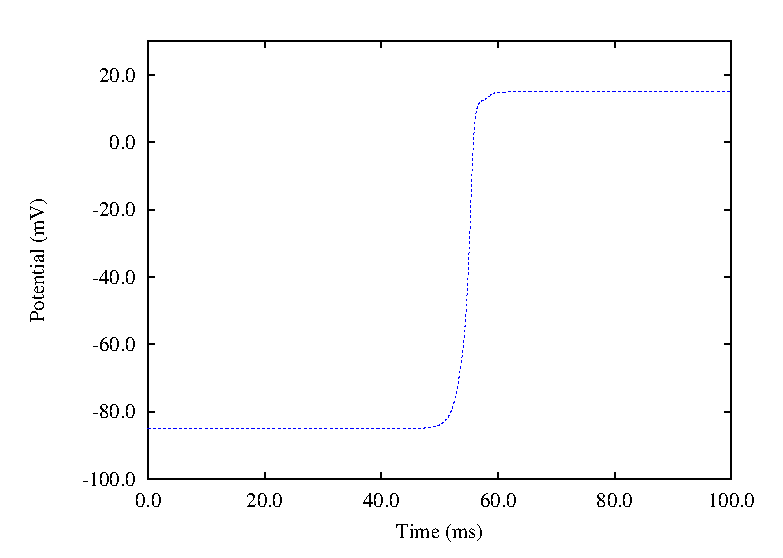
\includegraphics[width=75mm]{cardiac_electrophysiology/epsfiles/CubicVm.eps}
  \caption[Potential trace from a single cell using the cubic ionic current
  model]{Potential trace from a single cell using the cubic ionic current
    model}
  \label{fig:cubic_cell_traces}
\end{figure}
The polynomial models have roots at $V_r$, $V_{th}$ and $V_p$ causing any
stimulus under $V_{th}$ to return to rest and any suprathreshold stimulus to
move to the plateau potential $V_p$.
%
%===================================================================
\subsection{The FitzHugh-Nagumo model}
\label{The_FitzHugh-Nagumo_Model}
%===================================================================
The FitzHugh-Nagumo model is based on the cubic excitation model but also includes a recovery
variable so both depolarisation and repolarisation may be modelled. The form
of the model used was adapted from \citet{rogers:1994a}. The model
normalises potential values to be between zero and one. The transmembrane
potential has been denoted by $u$ and is calculated as
\begin{equation}
  u = \dfrac{V_m - V_r}{V_p - V_r}
\end{equation}
where $V_p$ is the plateau potential and $V_r$ is the resting potential. The
threshold potential, $V_{th}$ was normalised in the same way.
and the threshold potential in the same way.
\begin{equation}
  \alpha = \dfrac{V_{th} - V_r}{V_p - V_r}
\end{equation}
A cubic polynomial is used to describe the course of excitation
\begin{equation}
  I_{ion} = c_1 u \pbrac{u - \alpha} \pbrac{u - 1} + c_2 \nu
  \label{eqn:FHN_excitation_equation}
\end{equation}
where $c_1$ is an excitation rate constant and $c_2$ is an excitation decay
constant. The $\alpha$ parameter represents the normalised threshold potential
value. The variable $\nu$ is a dimensionless time dependent recovery variable and is
calculated from the equation 
\begin{equation}
  \dby{\nu}{t} = b \pbrac{u - d \nu}
\end{equation}
where $b$ is a recovery rate constant and $d$ is a recovery decay
constant. Both of these constants are dimensionless. The parameter values which
were used in the FitzHugh-Nagumo model 
have been adapted to maintain unit consistency and are shown in
\tabref{tab:FitzHugh-Nagumo_Model_Params}. 
\begin{table}[hbtp] \centering
  \begin{tabular}{|c|c|c|}
    \hline
    \emph{Parameter} & \emph{Units} & \emph{Value} \\ 
    \hline
    \hline 
    $V_r$ & $\mV$ & $-85$ \\
    $V_{th}$ & $\mV$ & $-75$ \\
    $V_p$ & $\mV$ & $15$ \\
    $c_1$ & $\uA\unitseparator\mm^{-2}$ & $0.175$ \\
    $c_2$ & $\uA\unitseparator\mm^{-2}$ & $0.03$ \\
    $b$ & $\pms$ & $0.011$ \\
    $d$ & $dimensionless$ & $0.55$ \\
    $C_m$ & $\uF\unitseparator\mm^{-2}$ & $0.01$ \\
    $A_m$ & $\mm^{-1}$ & $200$ \\
    \hline
  \end{tabular}
  \caption[Typical parameters for the FitzHugh-Nagumo ionic current model]{Typical
    parameters for the FitzHugh-Nagumo ionic current model}
  \label{tab:FitzHugh-Nagumo_Model_Params}
\end{table}
Traces of both the action potential and the recovery variable for the
FitzHugh-Nagumo model over time are shown in \figref{fig:FHN_1_cell_traces}.
\begin{figure}[hbtp] 
  \centering
  \begin{subfigure}[b]{0.45\linewidth}
    \centering
    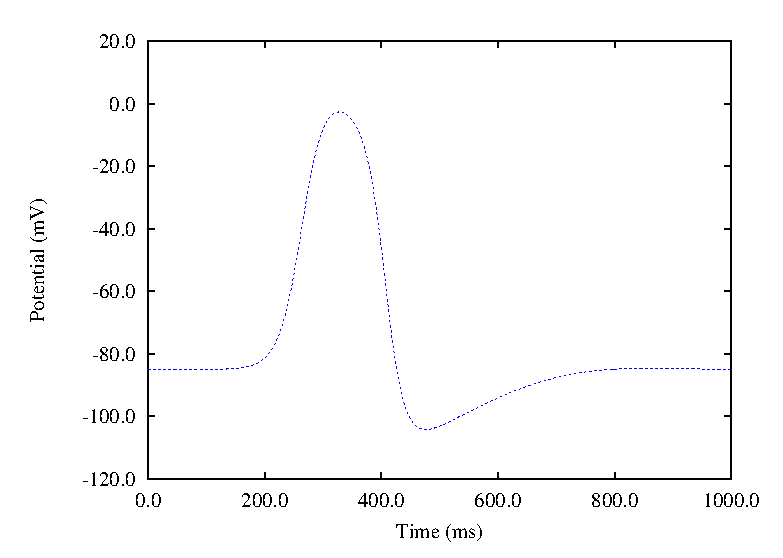
\includegraphics[width=\textwidth]{cardiac_electrophysiology/epsfiles/FHNVm.eps}
    \caption{}
  \end{subfigure}
  \hfill
  \begin{subfigure}[b]{0.45\linewidth}
    \centering
    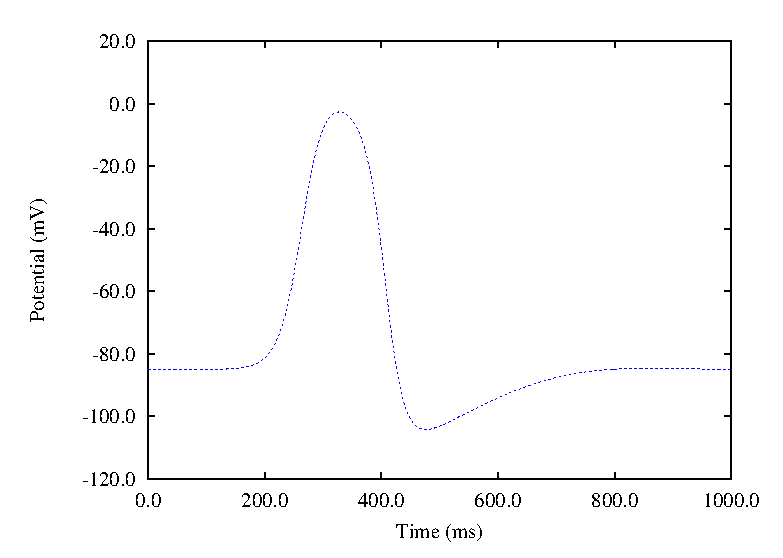
\includegraphics[width=\textwidth]{cardiac_electrophysiology/epsfiles/FHNVm.eps}
    \caption{}
  \end{subfigure}
  \caption[Traces from a single cell using the FitzHugh-Nagumo ionic current
  model]{Traces from a single cell using the FitzHugh-Nagumo ionic current
    model. Figure(a) shows the generated action potential and Figure(b) shows
    the recovery variable.}
  \label{fig:FHN_1_cell_traces}
\end{figure}
%
%===================================================================
\subsection{The modified FitzHugh-Nagumo model}
\label{The_modified_FitzHugh-Nagumo_Model}
%===================================================================
In the same paper as the original model was described \citet{rogers:1994a} described
some modifications to the model designed to generate a more realistic action
potential increasing the velocity of the upstroke and removing the large
hyperpolarization at the end of the action potential. The equation for the
ionic current was changed by multiplying the $c_2$ term by the normalised
potential. 
\begin{equation}
  I_{ion} = c_1 u \pbrac{u - \alpha} \pbrac{u - 1} + c_2 u \nu
  \label{eqn:mod_FHN_excitation_equation}
\end{equation}
The parameters which were used in the model were also updated. Alterations are
shown in \tabref{tab:mod_FitzHugh-Nagumo_Model_Params}.
\begin{table}[hbtp] \centering
  \begin{tabular}{|c|c|c|}
    \hline
    \emph{Parameter} & \emph{Units} & \emph{Value} \\ 
    \hline
    \hline 
    $c_1$ & $\uA\unitseparator\mm^{-2}$ & $0.26$ \\
    $c_2$ & $\uA\unitseparator\mm^{-2}$ & $0.1$ \\
    $b$ & $\pms$ & $0.013$ \\
    $d$ & $dimensionless$ & $0.8$ \\
    \hline
  \end{tabular}
  \caption[Adjusted parameters for the modified FitzHugh-Nagumo ionic current
  model]{Adjusted parameters for the modified FitzHugh-Nagumo ionic current model}
  \label{tab:mod_FitzHugh-Nagumo_Model_Params}
\end{table}
The resulting action potential and recovery variable traces are shown in
\figref{fig:FHNR_1_cell_traces}.
\begin{figure}[hbtp] 
  \centering
  \begin{subfigure}[b]{0.45\linewidth}
    \centering
    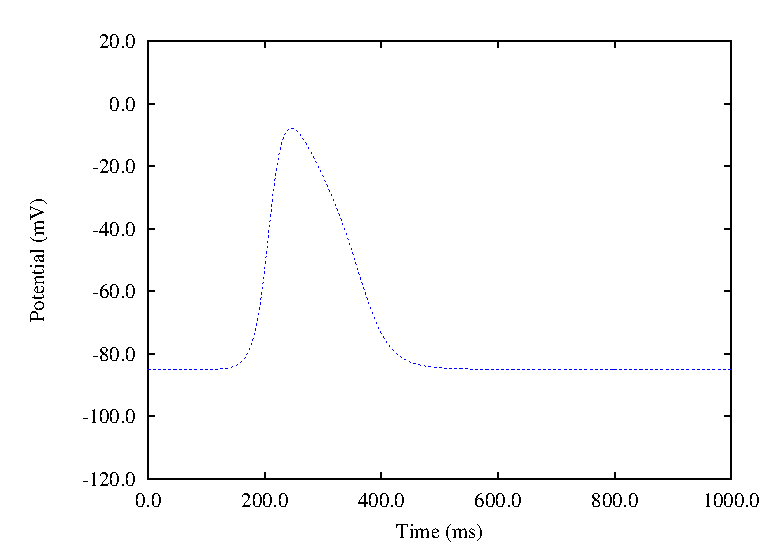
\includegraphics[width=\textwidth]{cardiac_electrophysiology/epsfiles/FHNRVm.eps}
    \caption{}
  \end{subfigure}
  \hfill
  \begin{subfigure}[b]{0.45\linewidth}
    \centering
    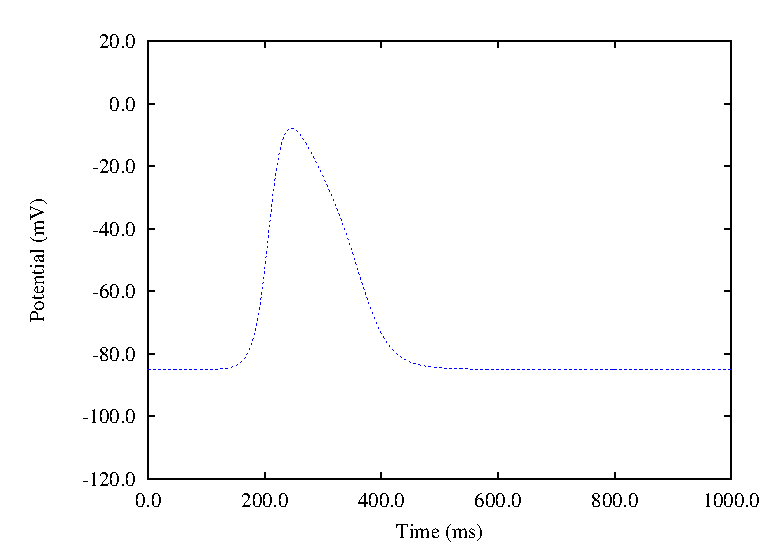
\includegraphics[width=\textwidth]{cardiac_electrophysiology/epsfiles/FHNRVm.eps}
    \caption{}
  \end{subfigure}
  \caption[Traces from a single cell using the modified FitzHugh-Nagumo ionic current
    model]{Traces from a single cell using the modified FitzHugh-Nagumo ionic current
    model. Figure(a) shows the generated action potential and Figure(b) shows
    the recovery variable.}
  \label{fig:FHNR_1_cell_traces}
\end{figure}
%
%===================================================================
\subsection{The van Capelle-Durrer model}
\label{The_van_Capelle-Durrer_Model}
%===================================================================
The van Capelle-Durrer model \cite{vancapelle:1980} follows the same general form as the
FitzHugh-Nagumo model with a single activation variable and a single recovery
variable but has the ability to add more complexity to the representation of
the parameters. The ionic current from the van Capelle-Durrer model is defined
to be
\begin{equation}
  I_{ion}=-Y \fnof{i_1}{V_m} - \pbrac{1-Y}\fnof{i_0}{V_m}
\end{equation}
where $\fnof{i_0}{V_m}$ and $\fnof{i_1}{V_m}$ are defined to be voltage
dependent currents and $Y$ is 
a dimensionless excitability parameter defined to be 
\begin{equation}
  \dby{Y}{t}=\dfrac{1}{T}\pbrac{\fnof{Y_{\infty}}{V_m}-Y}
\end{equation}
The $T$ parameter is a dimensionless time constant which may be used to easily scale the
duration of the action potential and $\fnof{Y_{\infty}}{V_m}$ is a voltage dependent
dimensionless variable which is the final value of the $Y$ parameter. In this
implementation of the model the $\fnof{Y_{\infty}}{V_m}$ was defined to be a piecewise
function. 
\begin{gather}
  \label{eqn:three_cases_of_Y_VCD}
  \begin{aligned}
  \fnof{Y_{\infty}}{V_m} &=
  \begin{cases}
    0 & \text{if $V_m < -80\mV$} \\
    1 & \text{if $V_m > -60\mV$} \\
    \pbrac{V_m+80}/20 & \text{otherwise}
  \end{cases}
  \end{aligned}
\end{gather}
A piecewise function was also chosen to represent $\fnof{i_1}{V_m}$.
\begin{gather}
  \label{eqn:three_cases_of_i1_VCD}
  \begin{aligned}
  \fnof{i_1}{V_m} &=
  \begin{cases}
    0.05+0.005\pbrac{V_m+70} 
      & \text{if $V_m < -70\mV$} \\
    0.06+0.00425V_m 
      & \text{if $V_m > 0\mV$} \\
    0.05+0.01\pbrac{V_m+70}/70 
      & \text{otherwise}
  \end{cases}
  \end{aligned}
\end{gather}
The $\fnof{i_0}{V_m}$ was not represented directly, instead it was defined to
be $\fnof{i_0}{V_m}=\fnof{i_1}{V_m}+\fnof{f}{V_m}$ where $\fnof{f}{V_m}$ was
defined by a piecewise function.
\begin{gather}
  \label{eqn: three_cases_of_f_VCD}
  \begin{aligned}
  \fnof{f}{V_m}=
  \begin{cases}
    0.0784+0.02\pbrac{V_m+74.3} 
      & \text{if $V_m < -74.3\mV$} \\
    -0.9884+0.0171\pbrac{V_m+27.8} 
      & \text{if $V_m > -27.8\mV$} \\
    a_fV_m^3+b_fV_m^2+c_fV_m+d_f 
      & \text{otherwise}
  \end{cases}
  \end{aligned}
\end{gather}
where
\begin{align*}
  a_f=& 3.837854\times 10^{-5}\\
  b_f=& 5.84649\times 10^{-3}\\
  c_f=& 0.2531834\\
  d_f=& 2.356256
\end{align*}
In this model $\fnof{i_0}{V_m}$, $\fnof{i_1}{V_m}$ and $\fnof{f}{V_m}$ have
units of $\uA\unitseparator\mm^{-2}$. The parameters used in the model are
given in \tabref{tab:VCD_Model_Params}.
\begin{table}[hbtp] \centering
  \begin{tabular}{|c|c|c|}
    \hline
    \emph{Parameter} & \emph{Units} & \emph{Value} \\ 
    \hline
    \hline 
    $V_m\pbrac{initial}$ & $\mV$ & $-78.6$ \\
    $Y\pbrac{initial}$ & $dimensionless$ & $0.07$ \\
    $T$ & $\ms$ & $50$ \\
    $C_m$ & $\uF\unitseparator\mm^{-2}$ & $0.01$ \\
    $A_m$ & $\mm^{-1}$ & $200$ \\
    \hline
  \end{tabular}
  \caption[Typical parameters for the van Capelle-Durrer ionic current model]{Typical
    parameters for the van Capelle-Durrer ionic current model}
  \label{tab:VCD_Model_Params}
\end{table}

Traces of both the action potential and the recovery variable $Y$ are shown in
\figref{fig:VCD_1_cell_traces}.  
\begin{figure}[hbtp] 
  \centering
  \begin{subfigure}[b]{0.45\linewidth}
    \centering
    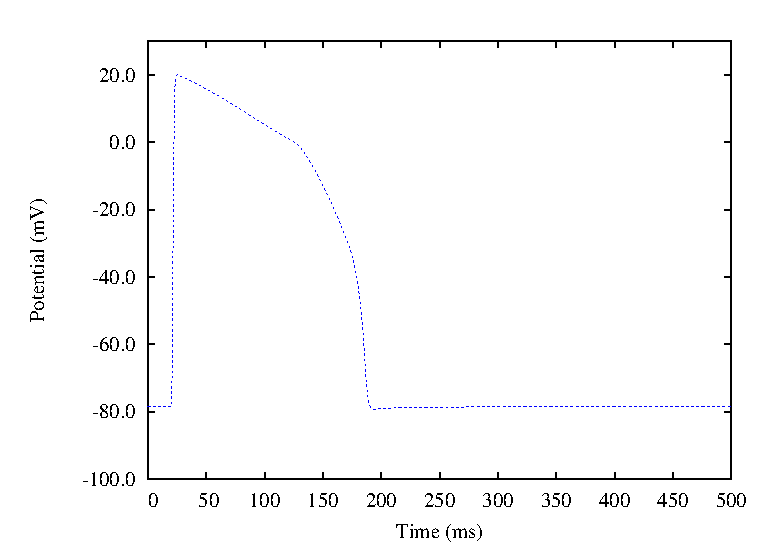
\includegraphics[width=\textwidth]{cardiac_electrophysiology/epsfiles/VCDVm.eps}
    \caption{}
  \end{subfigure}
  \hfill
  \begin{subfigure}[b]{0.45\linewidth}
    \centering
    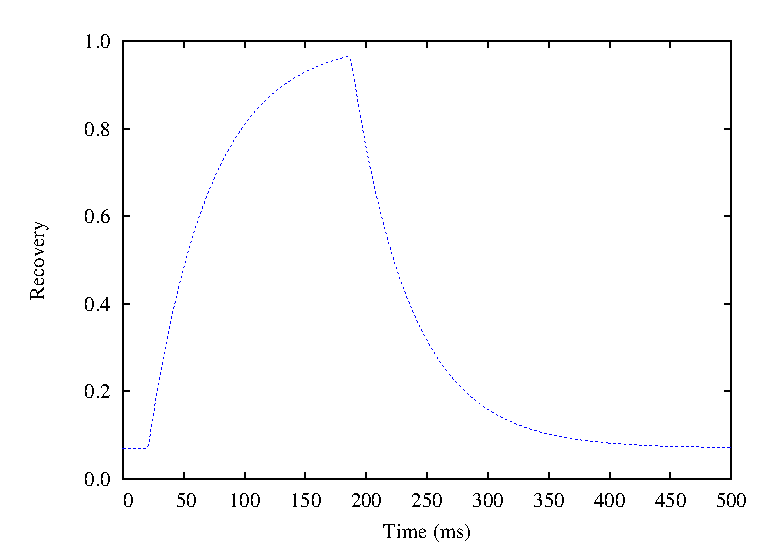
\includegraphics[width=\textwidth]{cardiac_electrophysiology/epsfiles/VCDRecov.eps}
    \caption{}
  \end{subfigure}
  \caption[Traces from a single cell using the van Capelle-Durrer ionic current
  model]{Traces from a single cell using the van Capelle-Durrer ionic current
    model. Figure(a) shows the generated action potential and Figure(b) shows
    the recovery variable.}
  \label{fig:VCD_1_cell_traces}
\end{figure}




\section{The Bidomain Model}
\label{sec:bidomain-model}

The complete model of cardiac activation would be one in which an
accurate model is formulated for each type of muscle cell.  The model
would completely describe the structure of the cell and detail every
aspect of its electrophysiological function down to a molecular level,
as well as the mechanical and energetic processes involved if this
information was required.  This cellular model would then be inserted
into an anatomically accurate description of the global cardiac
geometry, and solved on a cell-by-cell basis over the cardiac volume.
There are many reasons why such a model has not yet been constructed.
Firstly, it is difficult to obtain an accurate model of cell function.
Many of the membrane processes are still being quantified, if they are
known at all.  Secondly, an anatomically accurate definition of the
cardiac geometry is still incomplete.  Difficulties exist in measuring
the position of the ventricular endocardium, and many models only
describe the ventricular myocardium but not the atrial tissue or
accessory structures.  Coupled with this is a lack of a complete
description of the cellular structure.  The Auckland model is the most
detailed and accurate ventricular microstructural model to date, yet
it has little information on the Purkinje network, and none at all on
the atrial tissues.  The process of propagation is again only
partially understood, and a model describing even the conductivities
in the orthogonal microstructural directions is yet to be formulated.
Similar models of the energetic function and the passive and active
mechanics are still under construction, and the concept of being able
to couple the various components together in a total model is only
beginning to be looked at.  Even given the availability of this vast
amount of information, there would still be one requirement lacking.
Existing computational resources are barely adequate to solve a small
region of tissue.  \citet{spach:pilkington:1993} have developed a
model solving activation equations for individual cells for a
two-dimensional sheet model containing between 25,000 and 85,000
cells.  Even though there is only a small number of cells in a 2D
preparation, and the ionic model used is not the most complex
presently available, the model requires the use of a high-performance
supercomputer in order to solve the problem.  While computational
speeds are doubling approximately every eighteen months, a complete
model involving all cardiac processes is still a long way from being
computationally tractable.  Given that the current state of knowledge
and the current computational capabilities preclude the use of a model
completely representing the current state of knowledge of cardiac
activation, we need to determine what level of detail is feasible yet
sufficiently realistic so as to allow the investigation of various
abnormal phenomena.  The empirical models are no longer appropriate as
they ignore the cellular processes.  One commonly used method is to
use a macroscopic model which uses a volume-averaged approach, known
as the \emph{bidomain model}.  This model averages the electrical
properties over some length scale which is greater than that of a
single cell.  In doing this with an appropriate choice of length
scale, the effect of cell junctions on propagation can be ignored, and
the discrete cellular structure may be replaced with a uniformly
continuous structure.  There are problems with this approach.  If
discrete cellular effects play a significant role in the propagation
of activation, then either this will need to be incorporated or a new
model will need to be constructed.  Alternatively, if a macroscopic
model can provide results which are a reasonable approximation to the
explicit microscopic model then the averaged model may be justified.

\subsection{Definition of the Bidomain Framework}

The physical arrangement of cardiac cells has led to the belief that the heart
has electrical properties that are the same as a syncytium.  Experimental work
by \citet{weidmann:1970} and \citet{clerc:1976} on mammalian cardiac
tissue confirmed that propagation either along the fibre axis or transverse to
it produced results like a one-dimensional cable.  Cable theory defines
propagation along a membrane between two distinct spaces.  By extending
standard one-dimensional cable theory to two or three dimensions gives rise to
the bidomain model.

The concepts behind the bidomain model were first proposed by
\citet{schmitt:1969} who suggested that two interpenetrating domains could
be used to describe cardiac tissue, one representing volume-averaged
quantities in the intracellular space and one for those of the extracellular
space.  A mathematical formulation of this proposal was constructed in several
theses and papers by \citet{tung:1978}, \citet{plonsey:1984},
\citet{miller:1978a} and others.  The bidomain model has been adopted by
many other researchers in one form or another due to its convenience and
simplicity.  The model is discussed more fully in review papers by
\citet{henriquez:1993} and \citet{plonsey:1987}.  

Different papers give different names to the various regions that are part of
the bidomain model.  The names that we have chosen reflect the generally
accepted definitions (as given by \citet{krassowska:1994}) which tie in
with those that physiologists would use to describe cellular structure.  When
developing an activation model which is designed to be coupled with other
models, it is necessary to maintain consistent definitions and distinctly
identify each region.

The bidomain framework defines two domains which make up the cellular matrix.
The \emph{intracellular domain}, given the subscript ``$i$'', is the region
inside the cells, and the \emph{extracellular domain} with subscript ``$e$''
is the region between cells.  These two domains are interpenetrating which
means that they coexist at all points in space.  Therefore the properties and
state of the tissue at each point have separate components related to each
domain with appropriate subscripts.  For example, a single point in space will
have a tensor quantity associated with it defining the conductivity in each of
the intracellular and extracellular spaces.  The intracellular and
extracellular domains are separated by the cell membrane at all points, and
all current flow between the two domains occurs solely through the cell
membrane.  Because of the continuum approach to the physiology of the tissue,
this transmembrane current is volume-averaged.  This averaging approach is
required so that a length scale can be chosen such that the averaging produces
little loss of information.  Additionally, a third domain may be defined
consisting of all regions outside of the cardiac muscle, such as the bath that
the tissue is in, or the tissues within the torso cavity.  This domain is
referred to as the \emph{extramyocardial (outside) region} and given the
subscript ``$o$''.  \citeauthor{krassowska:1994}'s paper simply refers to
this region as ``outside'', but in a coupled problem it is unsure whether this
should refer to a region outside the heart or outside the body.  This naming
convention is illustrated in \figref{fig:bidomain-diagram}.
\begin{figure}[tb]
  \begin{center}
    \leavevmode
    \input{electrocardiology/figs/bidomain-diagram.pstex}
    \caption[The bidomain model]{The bidomain model.}
    \label{fig:bidomain-diagram}
  \end{center}
\end{figure}

Some authors (including \citet{pollard:pilkington:1993},
\citet{henriquez:1993}, \citet{plonsey:1987} and others), define the
regions differently.  In particular, what we term the extramyocardial region
is defined as the extracellular space, and what we call the extracellular
domain is called the \emph{interstitial domain}, often with ``extracellular''
also written in parentheses afterwards.  This causes some confusion in the
definitions of what constitutes extracellular space, and is inconsistent with
the standard physiological definition of the extracellular matrix being the
connective support structure and myoplasm surrounding cells.  Therefore it
seems best not to use the term ``interstitial'' at all, but to reserve the
word ``extracellular'' for use in describing structure that is part of the
extracellular matrix, and use another term for the medium surrounding the
tissue, which in this case we have chosen to call ``extramyocardial''.  This
agrees also with the tissue definitions of \citet{clerc:1976} in his
study of tissue conductivities which is cited as a definition for these terms
by \citet{pollard:pilkington:1993}.  It is true that the extramyocardial
space is also technically extracellular, but it is not (by definition) part of
the cardiac tissue structure, and because it is often not used in many
bidomain simulations, it is sensible to use another name for this region.
Some authors\cite{plonsey:1987} also use the subscript ``$o$'' for the
extracellular space, but this seems much less standard, and is similarly
confusing.

The bidomain model describes current flow through the cell membrane in a
space-averaged sense.  Instead of modelling a discrete cellular structure, the
bidomain constructs a continuum model with effective conductivity tensors
which is governed by continuous partial differential equations.  

\subsection{Mathematical Derivation of the Bidomain Model}

The most substantial mathematical description of the bidomain model is found
in the review paper by \citet{henriquez:1993}, which presents a formal
definition of the model from its origins in the core conductor model, and
outlines many of the approximations that can be made under certain
assumptions.

The bidomain equations may be derived in several ways depending on what
variables are wanted to solve for. This derivation yields equations for the
extracellular potential and the transmembrane potential while it is also
possible to generate equations for the intracellular and extracellular
potentials. The key definition in the bidomain equations is the definition of the
potential difference across the cell membrane which is known as the
transmembrane potential and given the symbol $V_m$.
\begin{equation}
  V_m = \phi_i - \phi_e
  \label{eqn:Vm_init_definition}
\end{equation}
Here $\phi_i$ is the potential in the intracellular domain and $\phi_e$ is the
potential in the extracellular domain. A schematic diagram of a bidomain
system is shown in \figref{fig:bidomain-diagram}. Ohm's law was  used
to calculate the intracellular and extracellular current densities. It is
assumed that the only current flow between the 
extracellular and extramyocardial space occurs through the boundary conditions
imposed on the domains.
\begin{align}
  V=&JR \nonumber \\
  J=&\dfrac{1}{R} V 
  \label{eqn:Ohms_Law}
\end{align}
Here $V$ is a voltage, $J$ is a current and $R$ is a resistance. Voltages
result from potential gradients so $V=\grad{\phi}$ may be substituted. In
addition to this the $\dfrac{1}{R}$ term may be written as a conductivity,
$\sigma$ which has units of $\mS$. \Eqnref{eqn:Ohms_Law} is then written for
the two domains as 
\begin{align}
  J_i=& - \sigma_i \grad{\phi_i} 
  \label{eqn:J_i_from_Ohms_Law} \\
  J_e=& - \sigma_e \grad{\phi_e}
  \label{eqn:J_e_from_Ohms_Law}
\end{align}
The negative signs in \eqnref{eqn:J_i_from_Ohms_Law} and
\eqnref{eqn:J_e_from_Ohms_Law} are necessary to ensure that current flows are
in the correct direction from regions of high potential to areas of low
potential. Any current which leaves one domain must cross the cell membrane and flow
into the other domain. This means that the change in current density in each
of the domains must be equal in magnitude but opposite in sign. The change in
current density in each domain is also equal to the current density across the
membrane.
\begin{equation}
  - \dotprod{\grad}{J_i} = \dotprod{\grad}{J_e} = A_mI_m
  \label{eqn:equal_current_densities}
\end{equation}
Here $A_m$ is defined to be the surface to volume ratio of the cell membrane
with units of $\pmm$ and
$I_m$ is the transmembrane current density per unit area which has units of
$\mS\unitseparator\mm^{-2}$. Combining
\eqnref{eqn:J_i_from_Ohms_Law}, \eqnref{eqn:J_e_from_Ohms_Law} and
\eqnref{eqn:equal_current_densities}, two equations were generated which
represent the conservation of current densities.
\begin{align}
  \dotprod{\grad}{\pbrac{\sigma_i \grad{\phi_i}}} =& A_mI_m
  \label{eqn:current_dens_conserv_1} \\
  \dotprod{\grad}{\pbrac{\sigma_e \grad{\phi_e}}} =& -A_mI_m
  \label{eqn:current_dens_conserv_2}
\end{align}
This implies that
\begin{equation}
  \dotprod{\grad}{\pbrac{\sigma_i \grad{\phi_i}}} = 
  -\dotprod{\grad}{\pbrac{\sigma_e \grad{\phi_e}}}
  \label{eqn:current_dens_conserv_3}
\end{equation}
Subtracting $\dotprod{\grad}{\pbrac{\sigma_i \grad{\phi_e}}}$ from both sides yields
\begin{equation}
  \dotprod{\grad}{\pbrac{\sigma_i \grad{\phi_i}}} 
  -\dotprod{\grad}{\pbrac{\sigma_i \grad{\phi_e}}} =
  -\dotprod{\grad}{\pbrac{\sigma_e \grad{\phi_e}}} 
  -\dotprod{\grad}{\pbrac{\sigma_i \grad{\phi_e}}}
  \label{eqn:current_dens_conserv_4}
\end{equation}
Using \eqnref{eqn:Vm_init_definition}, \eqnref{eqn:current_dens_conserv_4} can
be rewritten as
\begin{equation}
  \dotprod{\grad}{\pbrac{\sigma_i \grad{V_m}}} = 
  -\dotprod{\grad}{\pbrac{\pbrac{\sigma_i + \sigma_e} \grad{\phi_e}}}
  \label{eqn:first_bidomain_equation}
\end{equation}
This equation is usually refered to as the one of the two bidomain
equations which is used to solve for the extracellular potential given a
transmembrane potential distribution. The current flow across the
membrane, $I_m$ may be described by a time dependent capacitive current and an
ionic current
\begin{equation}
  I_m = C_m \delby{V_m}{t} + I_{ion}
  \label{eqn:membrane_current_flow}
\end{equation}
where $C_m$ is a membrane capacitance per unit area and $I_{ion}$ is the sum
of all ionic currents. The models used to 
represent the ionic
current component are presented in
\secref{sec:biophysical_models_of_cardiac_cells} and
\secref{sec:Simplified_models_of_cardiac_cells}. Combining
\eqnref{eqn:current_dens_conserv_1} and \eqnref{eqn:membrane_current_flow}
gives the following equation.
\begin{equation}
  \dotprod{\grad}{\pbrac{\sigma_i \grad{\phi_i}}} =
   A_m \pbrac{C_m \delby{V_m}{t} + I_{ion}}
  \label{eqn:membrane_current_flow_conserv}
\end{equation}
To convert \eqnref{eqn:membrane_current_flow_conserv} to have $V_m$ as the
dependent variable, $\dotprod{\grad}{\pbrac{\sigma_i \grad{\phi_e}}}$ is
added and subtracted from the left hand side of the equation.
\begin{equation}
  \dotprod{\grad}{\pbrac{\sigma_i \grad{\phi_i}}} -
  \dotprod{\grad}{\pbrac{\sigma_i \grad{\phi_e}}} +
  \dotprod{\grad}{\pbrac{\sigma_i \grad{\phi_e}}} =
   A_m \pbrac{C_m \delby{V_m}{t} + I_{ion}}
  \label{eqn:membrane_current_flow_conserv2}
\end{equation}
Using \eqnref{eqn:Vm_init_definition}
\eqnref{eqn:membrane_current_flow_conserv2} may be expressed as 
\begin{equation}
  \dotprod{\grad}{\pbrac{\sigma_i \grad{V_m}}} +
  \dotprod{\grad}{\pbrac{\sigma_i \grad{\phi_e}}} =
   A_m \pbrac{C_m \delby{V_m}{t} + I_{ion}}
  \label{eqn:second_bidomain_equation}
\end{equation}
which is known as the second of the bidomain equations and is used to update
the transmembrane potential at each time. It is possible for an
external stimulus current to be applied to either domain which gives the two
bidomain equations as
\begin{align}
  \dotprod{\grad}{\pbrac{\pbrac{\sigma_i + \sigma_e} \grad{\phi_e}}} =&
  -\dotprod{\grad}{\pbrac{\sigma_i \grad{V_m}}} +I_{s1}\\
  \dotprod{\grad}{\pbrac{\sigma_i \grad{V_m}}} +
  \dotprod{\grad}{\pbrac{\sigma_i \grad{\phi_e}}} =&
   A_m \pbrac{C_m \delby{V_m}{t} + I_{ion}} -I_{s2}
  \label{eqn:starting_bidomain_equations}
\end{align}
The extracellular domain is sometimes assumed to be highly conducting or the
domains are assumed to be equally anisotropic in an
effort to reduce the bidomain equations to a single domain hence reducing the
amount of computational effort required to solve the problem. The reduced
equation is known as the monodomain equation and is written as
\begin{equation}
  \dotprod{\grad}{\pbrac{\sigma \grad{V_m}}} =
   A_m \pbrac{C_m \delby{V_m}{t} + I_{ion}} -I_{s}
  \label{eqn:starting_monodomain_equation}  
\end{equation}
where the transmembrane potential is equal to the intracellular potential as
the extracellular potential is effectively zero. The conductivity values in
both the monodomain and bidomain equations are represented at each point in
space by a tensor containing conductivities in the fibre, sheet and cross
sheet directions allowing spatially varying fully orthotropic conductivities
to be modelled. 
%
%===================================================================
\subsubsection{Boundary conditions}
%\label{sec:bidomain_Boundary_conditions}
%===================================================================
There has been some differences in the literature in the boundary conditions
which have been applied to the bidomain model \citet{krassowska:1994}. The boundary
conditions used here are the original boundary conditions specified
by \citet{tung:1978} and confirmed by \citet{krassowska:1994}. There is assumed to be no
current flow between the intracellular and extramyocardial domains so the
boundary condition applied to the boundaries on intracellular space may be
written as
\begin{equation}
  \dotprod{\sigma_i \grad \phi_i}{\vect{n}}=0
  \label{eqn:orig_int_bc}
\end{equation}
where $n$ is a unit outward normal vector. The $\phi_i$ parameter was not
explicitly represented in the formulation of 
the bidomain equations so the boudary condition was modified to become a
boundary condition on $V_m$ using \eqnref{eqn:Vm_init_definition}. Taking
gradients, multiplying through by $\sigma_i$ and then taking dot products with
a normal vector, 
\eqnref{eqn:Vm_init_definition} becomes
\begin{equation}
  \dotprod{\sigma_i \grad V_m}{\vect{n}} = \dotprod{\sigma_i \grad \phi_i}{\vect{n}} -
  \dotprod{\sigma_i \grad \phi_e}{\vect{n}} 
\end{equation}
where \eqnref{eqn:orig_int_bc} demonstrates the $\phi_i$ term to be zero so
the actual boundary condition on the transmembrane potential becomes
\begin{equation}
  \dotprod{\sigma_i \grad V_m}{\vect{n}} = -\dotprod{\sigma_i \grad \phi_e}{\vect{n}} 
  \label{eqn:actual_int_bc}
\end{equation}
The boundary conditions on the extracellular domain were set up as a current
balance between the domain and the surrounding extramyocardial regions. 
\begin{equation}
  \dotprod{\sigma_e \grad \phi_e}{\vect{n}}=-\dotprod{\sigma_o \grad \phi_o}{\vect{n}}
  \label{eqn:orig_ext_bc}
\end{equation}
The negative sign accounts for the direction of current flow where both sides
of the equation use the same unit normal vector. The boundary extracellular
potentials must also match the boundary extramyocardial potentials. 
\begin{equation}
  \phi_e = \phi_o
\end{equation}
If the tissue is not
surrounded by a medium combinations of flux and potential boundary conditions
may be used to represent the desired setup. For a bidomain simulation with
equal anisotropy ratios an analytic potential boundary condition \citet{henriquez:1993}
may be set which is equal to
\begin{equation}
  \phi_e=-\dfrac{\sigma_{if}\sigma_{ef}}{\sigma_{if}+\sigma_{ef}}
\end{equation}
where $\sigma_{if}$ is the intracellular conductivity in the fibre direction
and $\sigma_{ef}$ is the extracellular conductivity in the fibre direction.
The boundary condition which was applied to the monodomain equation stated
that there was no current flow out of the myocardial domain because no
connection exists between the intracellular domain and any surrounding medium.
\begin{equation}
  \dotprod{\sigma \grad V_m}{\vect{n}}=0
\end{equation}
%The reaction part of the bidomain equations was represented by $I_{ion}$ which
%is usually highly nonlinear. 


\clearemptydoublepage
\chapter{Electrocardiography}

\section{Cardiac Anatomy and Function}

The description of cardiac physiology given here is only a basic outline,
with greater detail only on a few points which are relevant to the problem of
activation modelling.  For a more in-depth coverage of this subject, a
textbook such as \textsc{Physiology} Section V: The Cardiovascular System
\cite{zzz-berne:1988} should be consulted, or for a more specific look
at only the heart, refer to \textsc{Physiology of the Heart}
\cite{katz:1992}.

\subsection{Macroscopic description}

The heart is situated near the centre of the chest cavity between the right
and left lungs, and is supported inside a membranous structure, the
pericardial sac.  There are four major chambers in the heart and various
accessory tissues as shown in \figref{fig:heart-cross-section}.  The heart is
divided into left and right halves by the interventricular septal wall, such
that that there are no internal connections between the opposing chambers.
The larger lower chambers are the \emph{ventricles} (the left and right
ventricles are abbreviated as ``LV'' and ``RV'' respectively) and the smaller
upper chambers are the left and right \emph{atria} (given abbreviations ``LA''
and ``RA'').  The bottom of the ventricles is called the \emph{apex} and the
top of the ventricles is known as the \emph{base}.

\pstexfigure{electrocardiology/figs/heart-opened.pstex}{}{Longitudinal
  cross-section of the heart.  From \protect\citet[Fig~1.1,
  p.~3]{katz:1992}.}{fig:heart-cross-section}{}

Blood returns to the heart from the rest of the body via the superior and
inferior vena cava and enters the right atrium.  It flows from this chamber
into the right ventricle which pumps the blood to the lungs via the pulmonary
artery where the blood is oxygenated through the diffusion of oxygen across
the alveolar membrane.  The blood then returns to the heart through the
pulmonary vein and enters the left atrium, passes into the left ventricle, and
is subsequently pumped via the aorta to the rest of the body.  For this reason
the left ventricle is considerably larger than the right, and exhibits a
greater change in pressure during the cardiac cycle.  The period during which
the heart is being filled with blood is called \emph{diastole}, and the period
of contraction during which blood is pumped from the heart into the lungs and
circulatory system is called \emph{systole}.  The flow of blood from the RA to
the RV is controlled by the tricuspid valve, and the mitral valve controls
blood flow between the LA and LV.  The pulmonary valve is at the outflow tract
of the RV into the pulmonary artery, and the aortic valve at the connection of
the aorta to the LV.

Papillary muscles in both the LV and RV tether the mitral and tricuspid valves
to the ventricular wall during systole.  The LV papillary muscles are large
protrusions from the endocardial wall, and occupy a significant portion of the
cavity, whereas the RV muscles are relatively small, and attached only by
their bases to the ventricular wall.  These muscles prevent the valves from
inverting and entering the atria during systole, but the opening of the valves
is solely due to the pressure difference between the chambers.  The pulmonary
and aortic valves are not tethered because they are only preventing blood flow
during the slower passive filling phase.

\subsection{Microscopic description}
\label{sec:microstructure}

Cardiac muscle cells or \emph{myocytes} are roughly cylindrical with a length
in human ventricular tissue of $80$ to $100 \um$ and a diameter of $10$ to $20
\um$, and are bounded by the cell membrane or \emph{sarcolemma}.  A
diagrammatic representation of the cell is given in \figref{fig:cardiac-cell}
and has been reconstructed from an electron micrograph.

\pstexfigure{electrocardiology/figs/cardiac-cell.pstex}{}{Diagram showing the
  structure of a cardiac muscle cell.  A capillary runs between two adjacent
  cells.  From \protect\citet[Fig~28--2, p.~432]{zzz-berne:1988}.} {fig:cardiac-cell}{}

There are two sets of filaments present in muscle cells: \emph{thin filaments}
composed of a globular protein called \emph{actin}, and \emph{thick filaments}
formed as an aggregate of a much larger protein called \emph{myosin}.  The
thick and thin filaments interdigitate to form a \emph{sarcomere} between the
thin filament tethering points at Z lines, and this sarcomere is the basic
contractile unit.  The myosin molecule is composed of a pair of heavy chains
which hinge outwards near the end of the chain and attached to the end of this
``tail'' are two globular ``heads'' and two pairs of light chains.  The tail
and heads are hinged with respect to the rest of the molecule which is buried
within the filament.  According to the most common theory of contraction,
these appendages, or \emph{crossbridges}, cause the thick and thin filaments
to move relative to each other according to the four-stage \emph{crossbridge
  cycle}.  An important compound involved in this process is ATP (adenosine
triphosphate) which is usually bound to myosin to its resting state due to the
very high affinity between them.  ATP inhibits the interaction of myosin with
actin.  The first stage of contraction is the hydrolysis of ATP to form ADP
(adenosine diphosphate) and $\mathrm{P_i}$ (inorganic phosphate), both of
which remain associated with myosin.  In this state, the myosin head interacts
with the actin to form the active complex \emph{actomyosin}.  The chemical
energy expended by dissociation of ADP and $\mathrm{P_i}$ from the complex
performs mechanical work: the motion of the crossbridge.  This allows ATP to
bind again to the myosin and dissociates the crossbridge and the thin
filament, returning to the resting state.  Each cycle causes the thick and
thin filaments to move by about $10$ \nm relative to each other.

A large number of sarcomeres are present in a single cell.  Cells are joined
end-to-end with other cells through intercalated disks and also branch and
interconnect with neighbouring, nearly parallel cellular strands.  Electrical
connection between adjacent cells is through gap junctions which are located
in the intercalated disks.  Additionally, there are several important internal
structures.  Due to the almost constant energy requirements of repeated
cellular contraction in the cardiac cell there are a large number of
mitochondria which provide oxygen to the cell.  A network of sarcoplasmic
reticulum (SR) provides a large region of uptake pumps which remove \ionCa
from the cellular matrix and stores it in the junctional SR (JSR) awaiting
release for enabling contraction.  Deep invaginations of the sarcolemma into
the fibre are known as the transverse tubular system or T-tubules.  This
system is used primarily to conduct the action potential down into the cell,
and additionally to transport components from the interstitial fluid
surrounding the cell deep into the cell, and is of particular importance in
the excitation-contraction coupling.

An averaged myocyte direction can be defined at any point, which is known as
the \emph{local fibre orientation}.  Early papers by
\citet{maccallum:1900} and \citet{mall:1911} investigating the 
muscular architecture of the
heart suggest that ventricular myocardium is an assembly of discrete muscle
layers arranged in nested shells, or discrete fibre
bundles\cite{legrice:1992}.  This view of the microstructure was generally
accepted until \citet{hort:1957} and \citet{streeter:1966}
 performed the
first quantitative measurements of fibre orientation and found a smooth
transmural variation in fibre angle, which led to the predominant view being
that myocardium is a \emph{uniformly continuous, transversely isotropic}
medium.  A uniformly continuous medium is one in which there are no
discontinuous changes in the local fibre orientation.  A transversely isotropic
medium is one in which the material structure is isotropic in all directions
orthogonal to the fibre.  In other words, the fibre orientation is the only
local measure of microstructural composition, and can be regarded as a local
axis of symmetry.

Later studies by \citet{streeter:1969} and others were more thorough and
tended to confirm this view.  \citet{streeter:1979} did acknowledge,
however, that the muscular architecture is discontinuous at both a macroscopic
and microscopic level.  There were some problems associated with the methods
used to produce these results, as measurements were made only at a limited
number of sites, and the measurement points could not be accurately located
within a standard ventricular geometry.

Measurements of fibre orientation at a large number of sites spread throughout
the ventricular myocardium were made by \citet{nielsen:1987} and
\citet{mclean:1987}.  Their approaches involved cutting the ventricles
into thick serial slices transverse to the base-apex axis.  These techniques
have problems, including difficulty in spatial registration between slices due
to distortion, and loss of detail through averaging.  \citet{mclean:1989}
measured fibre angles from both transverse and longitudinal slices, though the
fibre orientation could not, of course, be measured from two orthogonal slices
taken from the same heart.

Many of the problems associated with earlier studies have been overcome in the
work of \citet{legrice:1992}, which, building on the techniques developed
by \citet{nielsen:1987}, is probably the most comprehensive and thorough
quantitative study of cardiac microstructure to date.
%\begin{figure}[tb]
%  \begin{center}
%    \leavevmode
%    \vspace{8cm}
%  \end{center}
%  \caption[Measurement rig]{Picture of the measurement rig used to measure
%    geometry and fibre angles.}
%  \label{fig:measurement-rig}
%\end{figure}
The approach used was to progressively remove thin layers of myocardium from a
mounted intact myocardium, preserving spatial registration.  This technique
allows measurement of fibre orientation throughout the ventricular wall, and
the absolute coordinates of each measurement point can be recorded for
alignment with the measured geometry.  This technique is a time-consuming
process when performed manually.  Details of this method and results are
outlined more fully in a paper by \citet{nielsen:1991a}.

Measurements obtained by Le Grice and coworkers are broadly consistent with
those reported by Streeter and others, but also reveal a new understanding of
the global nature of cardiac microstructure.  Their studies suggest that the
ventricular myocardium is not a uniform continuum, but rather a composite of
discrete layers of fibres, which are called \emph{sheets}
\cite{legrice:1992,legrice:1995a,smaill:glass:1991}.  Recorded fibre angles
are the edges of these branching sheets, and because fibres traverse the
sheets at a small angle, these measured angles are only projections of the
true angle.  However, \citet{streeter:1979} reports \emph{imbrication
  angles}\footnote{The imbrication angle (or sometimes \emph{embrication
    angle}) at the epicardium is the angle at which the fibre intersects the
  epicardial surface.  A value of $0\degree$ indicates a fibre orientation
  parallel to the surface.} at the epicardium (where the angles are greatest)
of only $3\degree$ to $5\degree$, so this variation is often ignored.

The sheets are on average four cells thick, and branching occurs between
layers, and the sheets are surrounded by a matrix of collagenous connective
tissue.  The nature and arrangement of the branching and of the connective
structure varies according to position within the ventricular wall.  Sheet
orientation is generally radial to the ventricular surfaces, though they
appear to become almost tangent to the epicardial surface.  A simple
structural model describing these features of the myocardium has been
developed by the Cardiac Research Group at the University of
Auckland\footnote{Department of Engineering Science, University of Auckland,
  New Zealand}, and details of the model are presented in several
papers,~\cite{hunter:pilkington:1993,hunter:panfilov:1996}.
\citet[p.3]{hunter:panfilov:1996} outline the model of ventricular
myocardium, which 
\begin{quote}
  $\ldots$ is represented as an interconnected hierarchy of muscle layers
  whose three-dimensional orientation varies through the ventricular wall.
  The extent of coupling between adjacent layers or sheets also varies
  transmurally to accommodate the changes in sheet orientation.  For a section
  cut tangential to the epicardial ventricular surface, the cut edges of the
  sheets define the fibre orientation.  Alternately, the cleavage planes
  revealed in transmural base-apex sections indicate the radial orientation of
  the sheets.
\end{quote}
\figref{fig:cardiac-microstructure} shows a schematic view of the cardiac
microstructure as predicted by this model.  No similar studies have yet been
made in which the nature of atrial tissue is investigated.
\pstexfigure{electrocardiology/figs/microstructure-schematic.pstex}{}
{Schematic of cardiac microstructure.  (a) Ventricular wall.  (b) A transmural
  block showing fibre orientation and branching sheet structures.  Note the
  transmural variation of fibre angle.  (c) The muscle fibres are bound by
  collagen fibres into sheets 3 to 4 cells thick.}{fig:cardiac-microstructure}{}

\subsection{Connective tissue structure}

There also exists a comprehensive organisation of extracellular connective
tissue, including a substantial hierarchy of collagen structures which
constrain the movement of the muscle fibres and sheets.  This constraining
network is more important when modelling mechanical behaviour than it is when
modelling electrical activation.  However, the constraints it places on the
microstructure will become significant as the electro-mechanical coupling is
investigated.  Various studies have begun to quantify the nature of the
connective tissues~\cite{caulfield:1979,mackenna:1994}.

\section{Activation}

Mechanical contraction of the heart is caused by the electrical activation of
the myocardial cells.  The heart is electrically self-contained, having the
ability to initiate its own beat with a regular period, and will continue to
beat after being removed from the body.  Cells capable of initiating
electrical activity are called \emph{pacemaker} cells, and exist in several
places throughout the heart.

\subsection{Normal Activation Sequence}

The normal sequence of activation is shown diagrammatically in
\figref{fig:activation-schematic}.
\pstexfigure{electrocardiology/figs/activation-sequence.pstex}{} {Schematic
  of the activation sequence.  From \protect\citet[Fig~27--23,
  p.~414]{zzz-berne:1988}}{fig:activation-schematic}{} Only those pacemaker
cells with the fastest rate of pacemaker discharge control the electrical
activity of the entire heart.  The region of tissue with the shortest period
of spontaneous electrical activity is the \emph{sinoatrial} (SA) node, which
is located on the atrial wall near the junction of the superior vena cava and
the right atrium, and consists of a group of pacemaker cells.  Action
potentials are normally generated here at the rate of $60$ to $100$ per
minute.  From the SA node, the action potential is propagated from cell to
cell through firstly the right atrium, followed closely by the left atrium at
a conduction velocity of approximately $1$ \mps until it reaches the
\emph{atrioventricular} (AV) node.  The AV node consists of similar
pacemaker-type cells as are found in the SA node, but because they beat
spontaneously at a slower rate (approximately $40$ to $55$ beats per minute)
they are governed by the propagation from the SA node.  In the event that the
SA node is removed or destroyed, or that conduction is slowed through the
atria, the cells in the AV node will take over as pacemaker for the heart.

Conduction through the AV node is at a much slower rate (around $0.05$ \mps)
giving time for the atria to contract and pump blood into the ventricles
before the action potential conducts through the ventricles and causes them to
contract.  The AV node is normally the only electrical connection between the
atria and the ventricles.  From the AV node, the electrical propagation enters
the \emph{bundle of His} which is the upper portion of the ventricular
conduction system and runs down the right side of the septum, and this common
bundle divides after a short distance into right and left \emph{bundle
  branches}.  The right branch continues down the right septal wall, and the
left perforates the septum and splits into two further main branches on the
left septal wall.  All of these branches continue to subdivide into a complex
network of fibres called the \emph{Purkinje fibre network}, spreading across
the endocardial surface of both ventricles and into the subendocardial region
of the ventricular myocardium.  Due to this arrangement of connecting fibres
the septum is activated first and normally pushes in towards the left
ventricular wall \cite{durrer:1970}.  The papillary muscles are also activated
early so that they can prevent the AV valves from inverting during systole.
Due to the faster conduction of approximately $2$ \mps through the
bundle and Purkinje fibres, the entire endocardium is excited almost
simultaneously.  The apical regions contract first and the basal regions are
usually the last regions to be excited.  Excitation spreads outwards through
the ventricular wall at a rate of about $0.3$ to $0.4$ \mps, and
the first epicardial region to be excited is the thinnest portion of the right
ventricular wall.  This activation process is summarised in
\tabref{tab:normal-activation}.
\begin{table}[tb]
  \begin{center}
    \leavevmode
%    \renewcommand{\tabularxcolumn}[1]{m{#1}}
%    \begin{tabularx}{\linewidth}{YYYY} \hline
     \begin{tabular}{p{3.5cm}p{3.5cm}p{3.5cm}p{3.5cm}} \hline
      \textsc{Normal sequence of activation} &
      \textsc{Conduction velocity} (\units{m \cdot sec^{-1}}) &
      \textsc{Time for impulse to traverse structure} (\units{sec}) &
      \textsc{Rate of pacemaker cell discharge} (\units{min^{-1}}) \\ \hline
      SA node & $< 0.01$ & $\top$ & $60$--$100$ \\
      $\downarrow$ & & $\sim 0.15$ & \\
      Atrial myocardium & $1.0$--$1.2$ & $\bot$ & None \\
      $\downarrow$ & & & \\
      AV node & $0.02$--$0.05$ & $\top$ & Most rapid in \\
      $\downarrow$ & & : & lower fibres: \\
      Bundle of His & $1.2$--$2.0$ & : & $40$--$55$ \\
      $\downarrow$ & & $\sim 0.08$ & \\
      Bundle branches & $\top$ & : & $\top$ \\
      $\downarrow$ & $2.0$--$4.0$ & : & $25$--$40$ \\
      Purkinje network & $\bot$ & $\bot$ & $\bot$ \\
      $\downarrow$ & & & \\
      Ventricular myocardium & $0.3$--$1.0$ & $\sim 0.08$ & None \\ \hline
%    \end{tabularx}
     \end{tabular}
  \end{center}
  \caption[Normal activation sequence]{Normal activation sequence.  (From
    \protect\citet[Table~20.1, p.~475]{katz:1992})}
  \label{tab:normal-activation}
\end{table}

The pressure and volume changes of the cardiac cycle are illustrated in
\figref{fig:press-vol2}.  They fall into a number of phases:
Isovolumetric contraction (the mitral valve closes and the pressure in the
ventricle rises rapidly.  Until the aortic valve opens, the volume of the
ventricle remains unchanged).  
Ejection (as soon as the aortic valve opens, blood is rapidly ejected from the
ventricle into the aorta.  This is followed by a phase of relatively slow ejection).
Isovolumetric relaxation (after ejection finishes, the aortic valve closes.
As the ventricle relaxes, the pressure within it falls rapidly, but until it
has fallen to the level present in the left atrium the volume in the ventricle
remains unchanged).
Ventricular filling (when the pressure in the ventricle falls below that in
the atrium, the mitral valve opens and a period of rapid ventricular filline
ensues.  This is followed by a slow phase, or diastasis, during which the
pressure rises slowly.  This continues until artial contraction propel more
blood through the mitral valave and causes a small increae in left ventricular
volume and pressure prior to the onset of the next ventricular systole).
\begin{figure}[htbp] \centering
  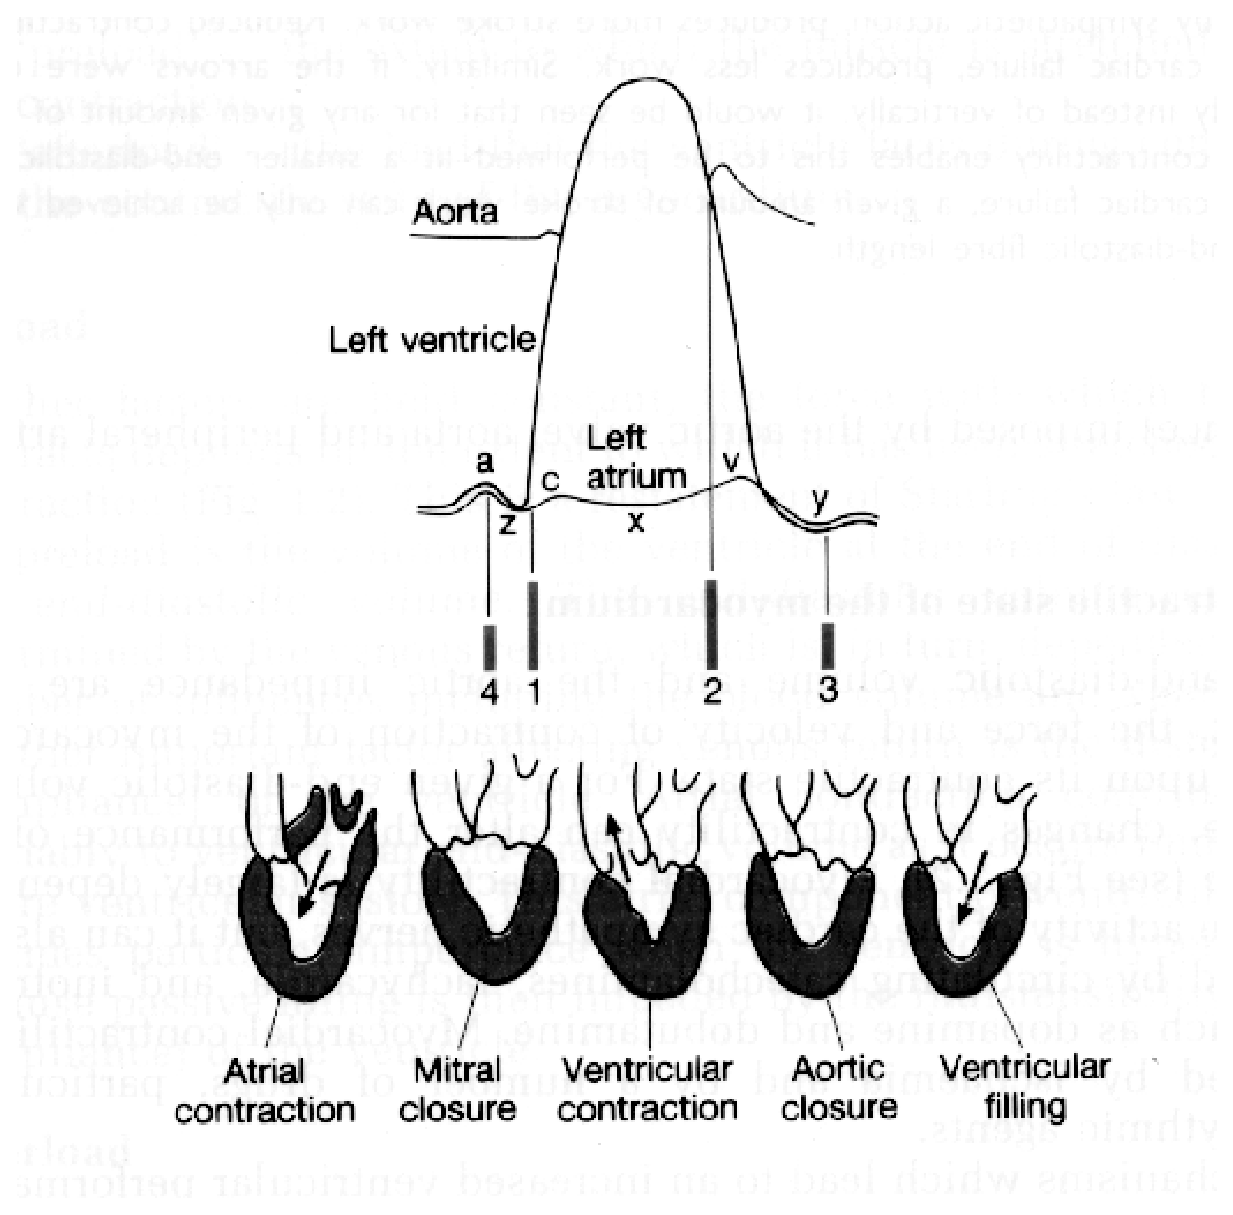
\epsfig{file=electrocardiology/epsfiles/press-vol2.eps,width=10cm}
  \caption{Pressure pulses in the left atrium, left ventricle and aorta}
  \label{fig:press-vol2}
\end{figure}

The relation between the pressure and the electrical impulse is shown in 
\figref{fig:press-vol}.
\begin{figure}[htbp] \centering
  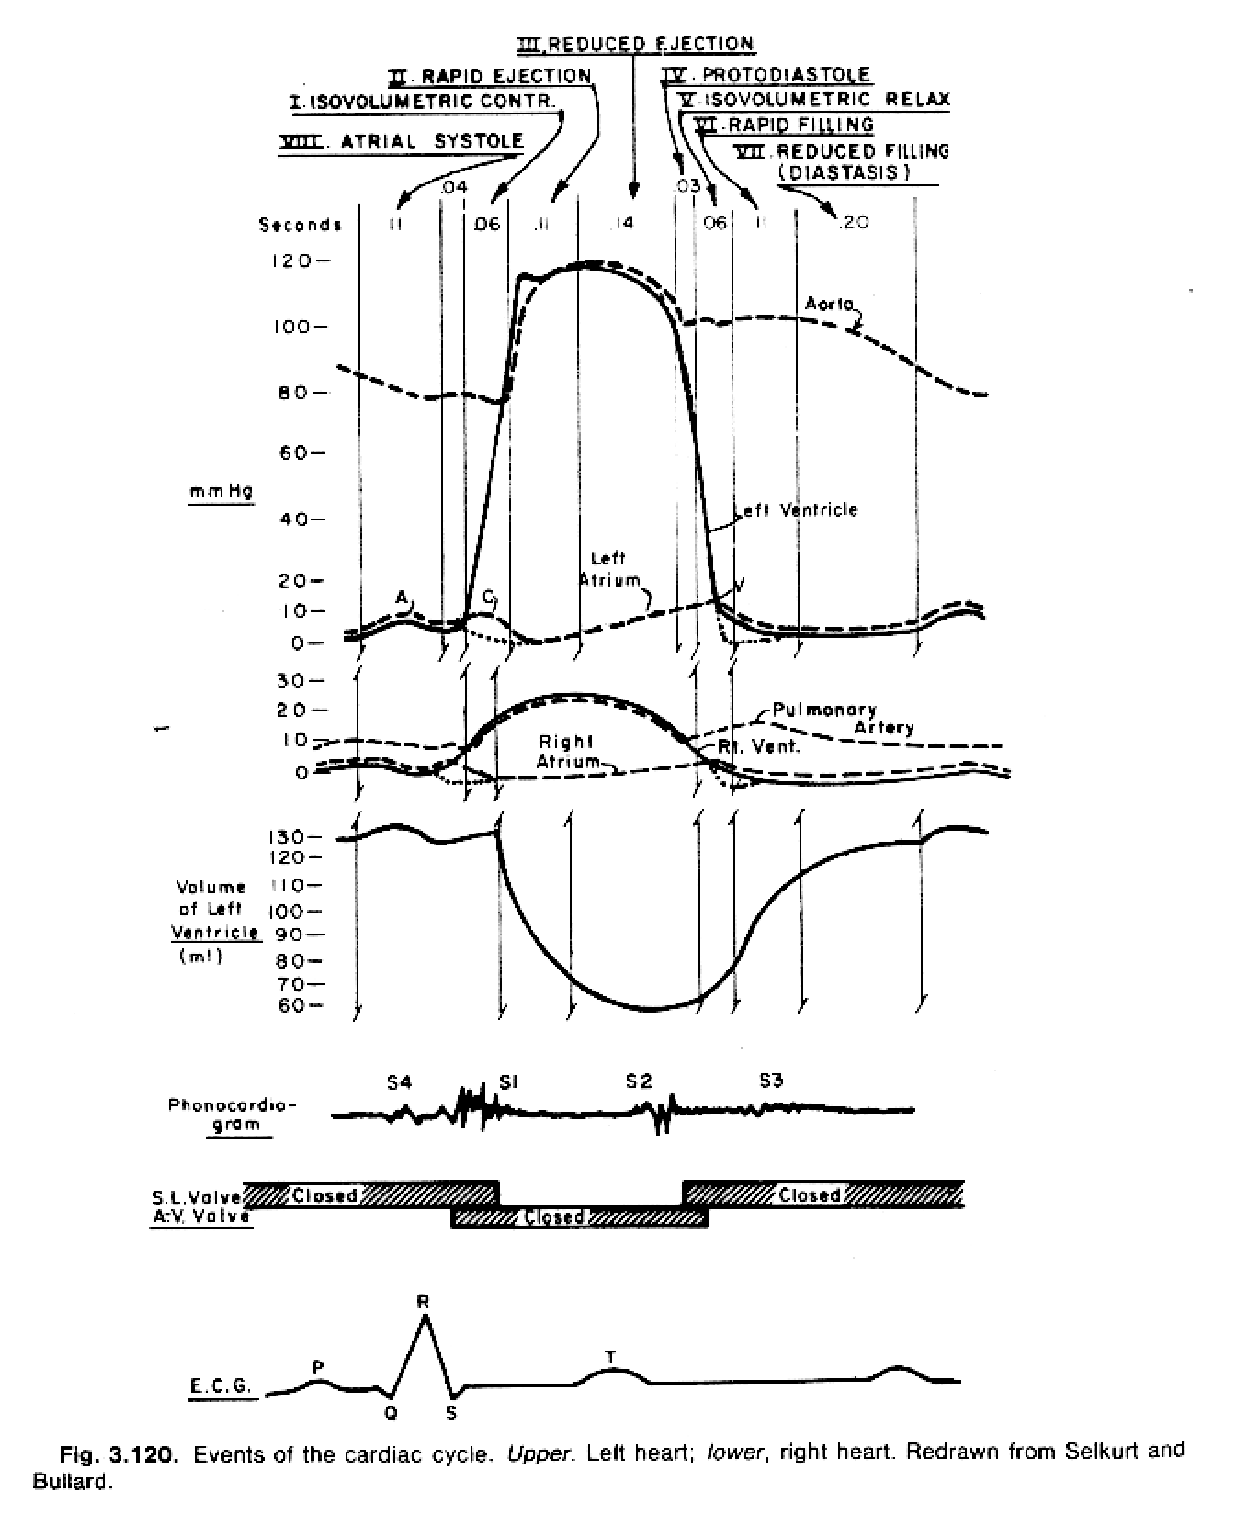
\epsfig{file=electrocardiology/epsfiles/press-vol.eps,width=10cm}
  \caption{Events of the cardiac cycle - pressure, volume and ECG}
  \label{fig:press-vol}
\end{figure}

\section{History of the ECG}
The bioelectric sources which arise during the heart's excitation process
produce a flow of electric current in the surrounding tissues.  It is
therefore possible to detect, with a pair of electrodes external to the heart,
time-varying potential differences known as electrocardiograms.

The first recording of a human ECG was by \citet{waller:1887}. The
electrical activity of the exposed heart was already known ( and galvanometers
had been invented) but Waller decided to investigate the possibility of
recording potentials from the limbs of animals and from man.  He dipped his
right hand and left foot into a couple of basins of salt solution which were
connected to two poles of an electrometer and ``at once had the pleasure of
seeing the mercury column pulsate with the pulsation of the heart''.

Waller demonstrated this at St Mary's Laboratory in 1887 and Professor Willem
Einthoven was in the audience (Waller often demonatrated the ECG on his dog
Jimmie standing in buckets of salt solution). It is Einthoven\footnote{Willem
  Einthoven was awarded the 1924 Nobel prize for Physiology or Medicine for
  the discovery of electrocardiogram mechanism} that most people credit with
the birth of the ECG (Einthoven acknowledges Waller as the first person to use
the word ECG) and Waller is overlooked.

Einthoven's major achievement was the invention of a device sensitive enough
to record \emph{potentials} from the body (as oppoesed to Waller who detected
\emph{voltages}).  Einthoven's first ECG machine weighed approximately 600
poinds and required 5 operators.

Einthoven is responsible for developing the theory on which the ECG is based
(e.g. Einthoven triangle, leads I, II, III, Einthoven equation). Einthoven's
notation for the ECG wave is still used.  A schematic ECG waveform is given in
\figref{fig:ECG}.  The letters P to U are used to denote certain parts of the
waveform and, as we will see in more detail later, they can be attributed to
different parts of the underlying cardiac activation.

\begin{figure}[htpb] \centering
  \input{electrocardiology/figs/ECG.pstex}
  \caption{`Standard' ECG (lead II waveform)}
  \label{fig:ECG}
\end{figure}

An ECG is recording (1) the spread of stimulus throught the heart muscle
(depolarisation) and (2) the return of the stimulated heart muscle to the
resting state (repolarisation).

\subsection{The Pathways of Conduction and the ECG}
As noted above, in the usual sequence of events, the electrical impulse arises in the sinus
node and spreads across the atria to reach the AV node. It can then only reach
the ventricles by passing into the rapidly conducting AV bundle and its
branches.

The first part of the ventricles to be activated is the septum, followed by
the endocardium.  Finally, the impulse spreads outwards to the epicardium.

The spread of the cardiac impulse gives rise to the main deflections of the
ECG: P, QRS and T waves.

\begin{itemize}
\item the \emph{P wave} is the first deflection of the cardiac cycle and
  represents atrial depolarisation;
\item the \emph{PR interval} represents the time taken for the cardiac impulse
  to spread over the atrium and through the AV node and His-Purkinje System;
\item the \emph{QRS complex} represents the spread of the depolarisation
  through the ventricles'
\item the\emph{T wave} represents the ventricular repolarisation.
\end{itemize}

There is still debate over the existence and interpretation of the U wave.

\subsection{Electrodes and Leads}
A conventional ECG consists of tracings from 12 leads. The
term `lead' refers to the ECG obtained as a result of recording the
difference in potential between a pair of electrodes.

\subsubsection{The bipolar (standard) leads} 
In these leads, the electrodes are
attached to the limbs. In lead I the positive electrode is attached to the
left arm  and the negative to the right arm. In lead II the positive
electrode is atttached to the left leg and the negative to the right arm.  In
lead III the positive is attached to the left leg and the negative to the
left arm. They may thus be depicted as :
\begin{itemize}
\item lead I = left arm minus right arm (LA -RA)
\item lead II = left leg minus right arm (LL-RA)
\item lead III = left leg minus left arm (LL-LA).
\end{itemize}
i.e.
\begin{eqnarray*}
  I & = & E_{L} - E_{R}\\
  II & = & E_{F} - E_{R}\\
  III & = & E_{F} - E_{L}
\end{eqnarray*}

These leads were the original leads that were used by Eintoven in his early
recordings. It can be deduced from these equations that lead II should be equal to the
sums of lead I and III i.e.
\begin{eqnarray*}
  I + III = II & & \mbox{(Einthoven's law)}
\end{eqnarray*}
.

Einthoven regarded each limb used in the recording of the bipolar ECG as an
apex of an equilateral triangle, equidistant electrically form the heart at
the centre\figref{fig:ET}. This idea is still used today in the interpretation
of ECGs, despite its obvious limitations (e.g. the body is not an electrically
homogenoeous sphere).

\begin{figure}[htpb] \centering
  \input{electrocardiology/figs/ET.pstex}
  \caption{Orientation of leads I,II,II - Eintovens triangle}
  \label{fig:ET}
\end{figure}


\subsubsection{Unipolar leads}
1934 saw the introduction of unipolar leads - so called because they represent
the potential variation of a single point.  In 1942 Goldberger modified these
to produce the so called augmented unipolar lead (done so the voltages were
easier to detect.
The unipolar leads have an exploring electrode placed on a chosen site linked with an
indifferent electrode with a very small potential. In an attempt to obtain a
central terminal with `zero potential', Wilson connected all three limb
electrodes through 5000 $\Omega $ resistances to form the indifferent
electrode.

\paragraph{Unipolar chest leads}
When unipolar leads are recorded from the chest wall, the exploring electrode
is connected to the positive pole of the ECG and the negative to the central
terminal. By convention, the following sites for the exploring electrode
 are normally selected (shown in\figref{fig:v1-v6}, \figref{fig:v1-v6-b}):
\begin{itemize}
\item V1, the fourth intercostal space just to the right of the sternum;
\item V2,  the fourth intercostal space just to the left of the sternum;
\item V3, midway between V2 and V4;
\item V4, the fifth intercostal space in th emidclavicular line;
\item V5, the left anterior axillary line at the same horizontal level as
  V4;
\item V6, the left mid-axillary line at the same horizontal level as V4
\end{itemize}

\begin{figure}[htbp] \centering
  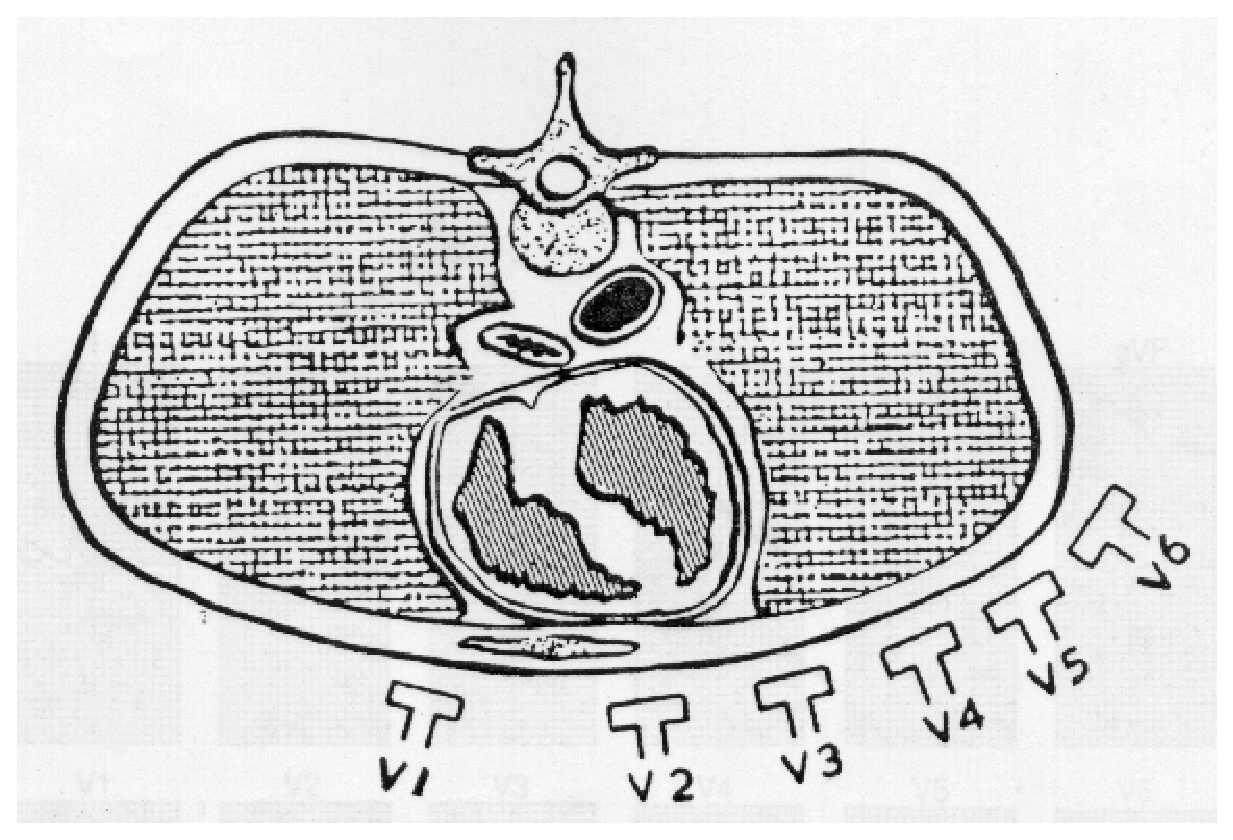
\epsfig{file=electrocardiology/epsfiles/v1-v6.eps,width=10cm}
  \caption{Diagram showing the orientation of the unipolar chest leads}
  \label{fig:v1-v6}
\end{figure}

\begin{figure}[htbp] \centering
  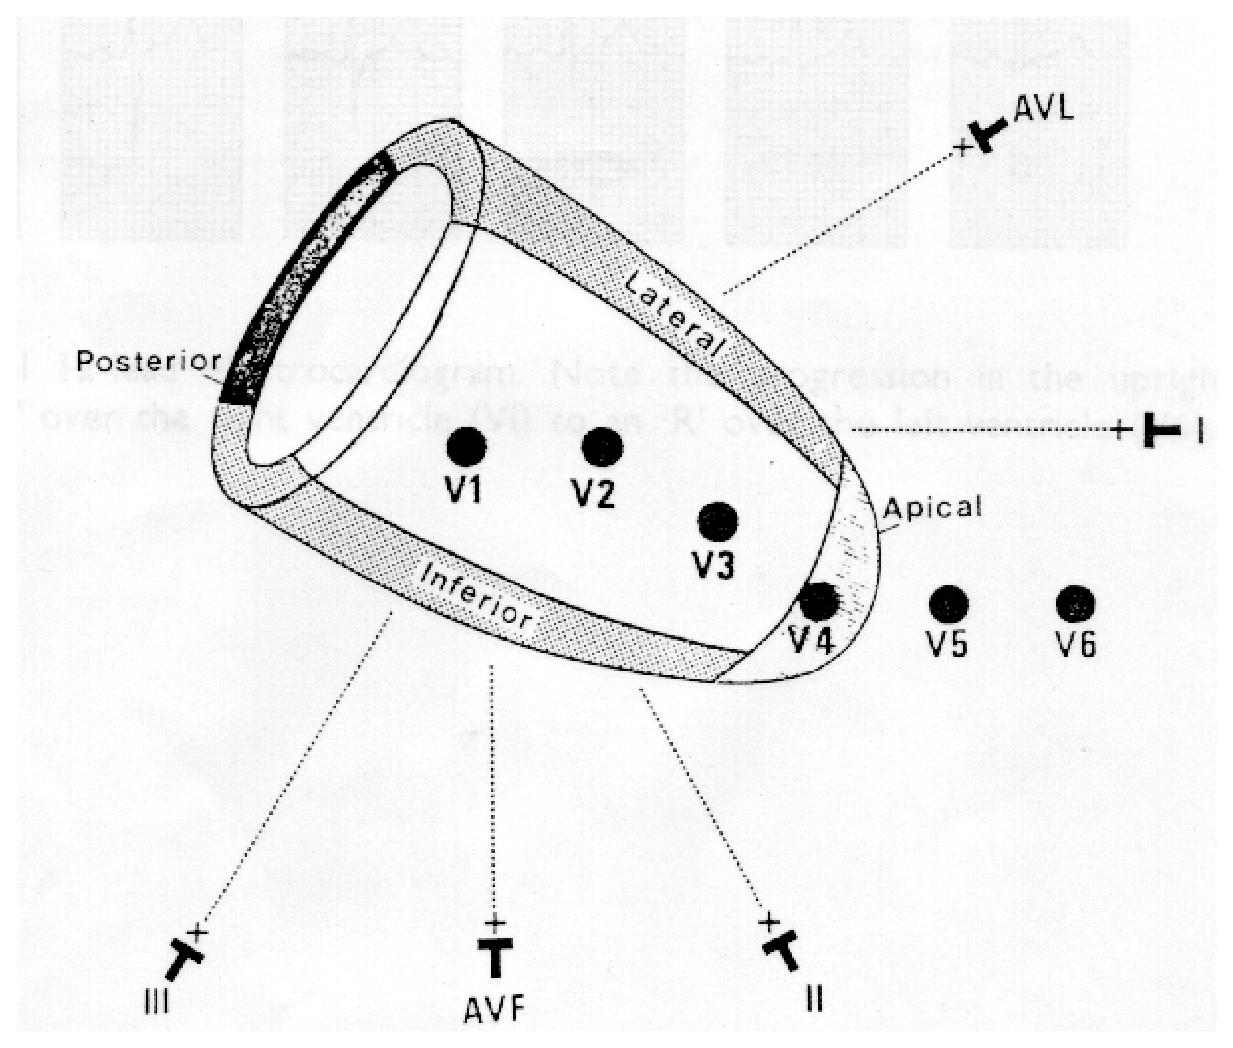
\epsfig{file=electrocardiology/epsfiles/v1-v6-b.eps,width=10cm}
  \caption{Diagram showing the orientation of the various leads to the left
    ventricular 'cone'.  Note that there is no lead which is oriented
    directly to the posterior wall of the heart}
  \label{fig:v1-v6-b}
\end{figure}

Additional leads can be taken from V3R and V4R, sites on the right side of
the chest equivalent to V3 and V4.  Occasionally, leads may be placed at
higher levels, e.g. the second, third or fourth intercostal spaces or
further laterally (V7 and V8).

\paragraph{Unipolar limbleads}
In these leads, the exploring electrode is placed on one limb, and the
negative pole is connected to Wilson's central terminal, modified by the
ommission of the connection from the limb under study to the central terminal
\figref{fig:ecg-leads}.

\begin{figure}[htbp] \centering
  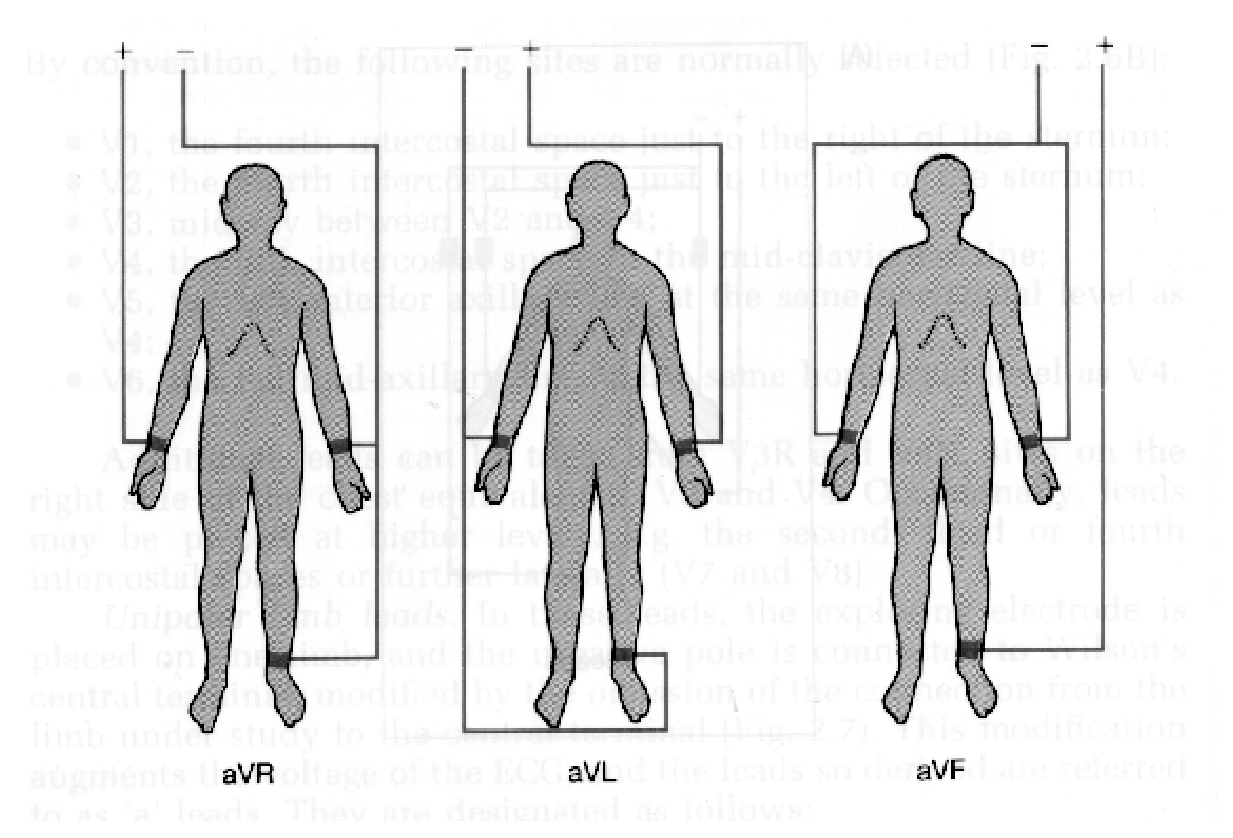
\epsfig{file=electrocardiology/epsfiles/ecgleads.eps,width=10cm}
  \caption{The attachment of unipolar limb leads.  Note that the limb under
    study is not attached to the central (negative) terminal}
  \label{fig:ecg-leads}
\end{figure}

This modification ``augments the voltage of the ECGs'', and the leads so derived
are referred to as 'a' leads. They are designated as follows:
\begin{itemize}
\item aVR, augmented voltage from the right arm;
\item aVL, augmented voltage from the left arm;
\item aVF, augmented voltage from the left foot.
\end{itemize}
If we consider each of these leads in a bit more detail then for aVR the
central terminal consists of the average of the voltages from L and F and aVR
is therefore
\begin{displaymath}
  aVR = E_{R} -\frac{1}{2} (E_{L} + E_{F} ) = -\frac{1}{2}(I + II)
\end{displaymath}
If an average of the potentials from V, L and F is used as the central
terminal (as in the original unipolar leads) then the voltage recorded, VR,
is only  $\frac{2}{3}aVR$ - hence the name ``augmented'' VR.
Similarly
\begin{eqnarray*}
  aVL = & E_{L} - \frac{1}{2} (E_{F} + E_{R}) & = I - \frac{1}{2} II\\
  aVF = & E_{F} - \frac{1}{2} (E_{L} + E_{R}) & = I \mp \frac{1}{2} I
\end{eqnarray*}
  
It can be seen, that once any 2 of the 6 extremity leads (I, II, III, aVR,
aVF, aVL) have been recorded the others can be deduced.

So the six extremity leads (I,I,II, aVR, aVL, aVF) show electrical voltage of
the heart transmitted onto a vertical plane while the 6 precordial leads show
voltages transmitted onto the horizontal plane.

\section{Basic Theory}

Einthoven's original model has proven extremely useful and still dominates
much of electrocardiography. Einthoven used a dipole to represent the heart
and postulated that the potentials at the limbs were related to the heart in
the same way that the potential at the 3 vertices of an equilateral triangle
places in an unbounded homogenous two dimensional volume conductor would be
related to a dipole source at the centre of the triangle. That is the heart
was modelled as a dipole and the body as part of a homogenous infinite
conductor.

More detailed models have been developed (taking into account inhomogeneities,
etc.) but the dipole model is still widely used (it is simple and reasonably
accurate).

The ECG shows \emph{projections} of this dipole in the direction of the leads.
At position 1, projection onto lead II is small and negative (Q wave). As the
``heart vector'' sweeps through positions 2,3 and 4 the projection onto lead
II is large and positive (the R complex). From 4 back to 0 the deflection
becomes small and negative (see \figref{fig:heart_vect_mb}).

\pstexfigure{electrocardiology/figs/HV.pstex}{}{Heart vector projections}{fig:heart_vect_mb}{}

More complicated models (which used quadrupoles, solid angles, etc.) give rise
to approximately the same thing.

The 12 different lead sites show the projection of the dipole along 12
different directions.


\section{The Normal ECG} 

\subsection{The Normal Electrocardiogram}
A normal 12 lead ECG recording is given in \figref{fig:normalecg}.  We discuss
below the significance of each part.
\subsubsection{The P Wave}
The normal P wave (\figref{fig:pwaves}~A) results from the spread of electrical activity across the
atria (the activity of the sinus node itself cannt be detected in the
ECG). Because the impulse spreads from right to left, the P wave is upright in
leads I,II and aVF, is inverted in aVR and may be upright, biphasic or
inverted in lead III,aVL and V1. It should not be higher than 3mm in the
bipolar leads or 2.5mm in the unipolar leads, or greater than 0.10 s in duration.

\begin{figure}[htbp] \centering
 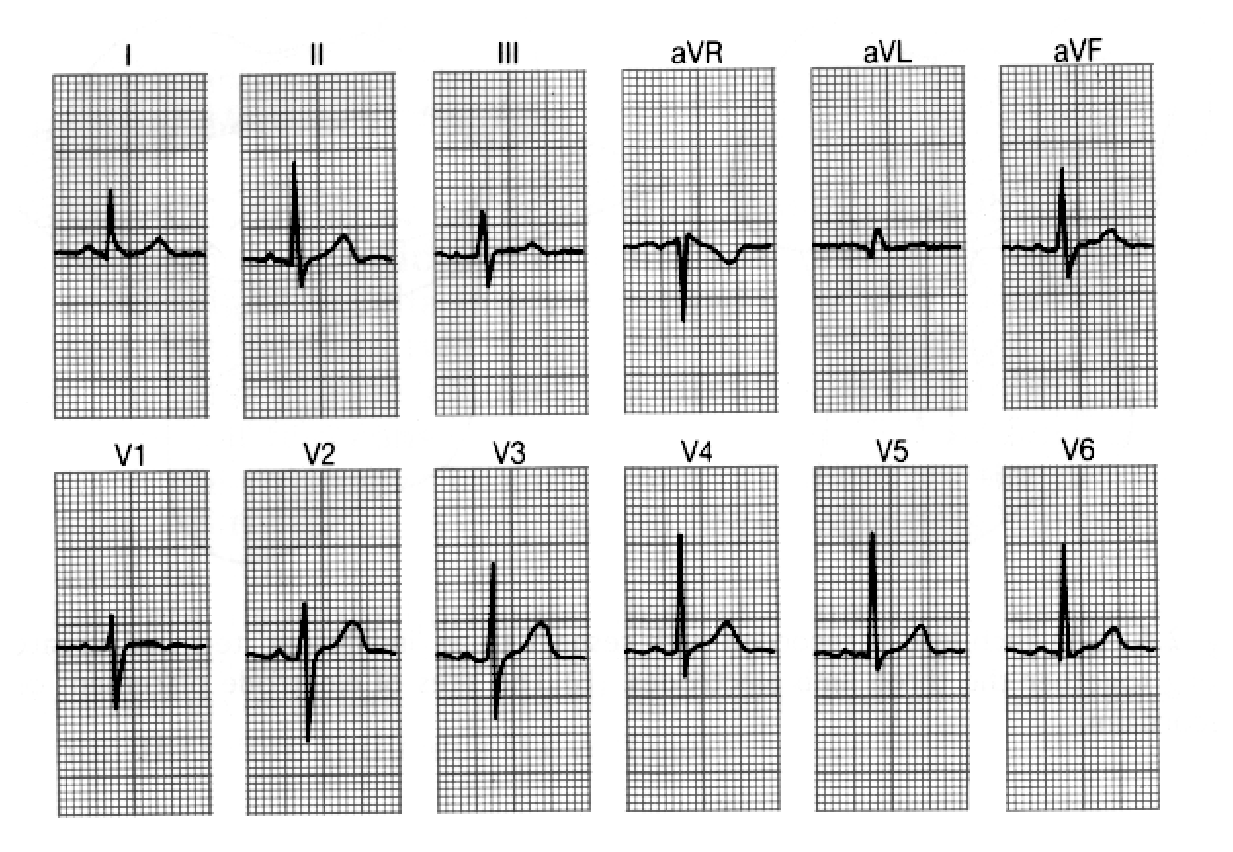
\epsfig{file=electrocardiology/epsfiles/normalecg.eps,width=10cm}
 \caption[Normal 12-lead electrocardiogram.]{Normal 12-lead
   electrocardiogram. Note the progression in the upright deflection from `r'
   over the right ventricle (V1) to an `R' over the left ventricle V6.}
 \label{fig:normalecg}
\end{figure}

\begin{figure}[htbp] \centering
 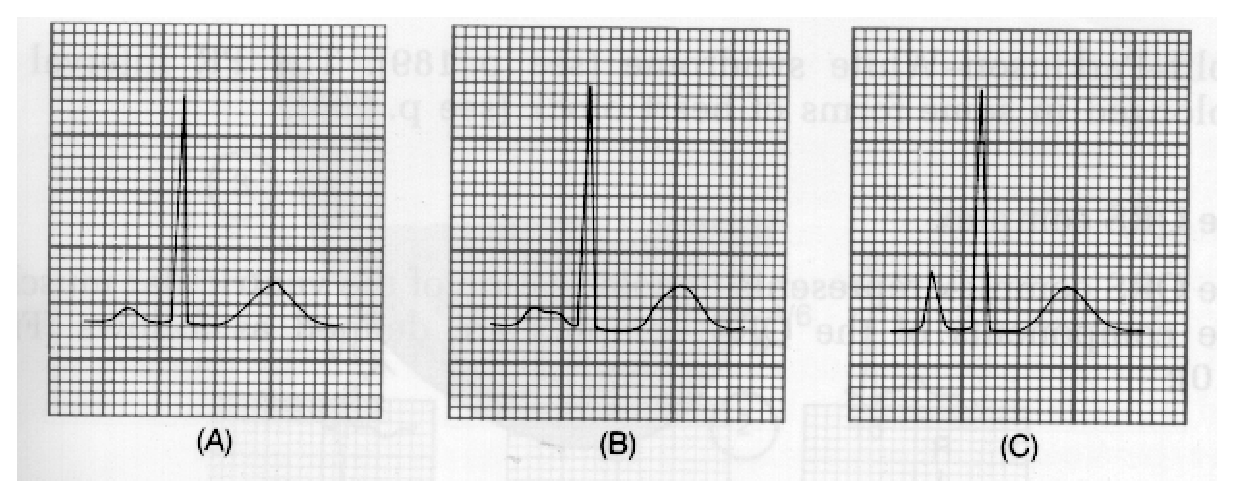
\epsfig{file=electrocardiology/epsfiles/pwaves.eps,width=10cm}
 \caption[P wave appearance in lead II.]{P wave appearance in lead II. (A) Normal. (B) Broadened and
   notched (P mitrale). (C) C Tall and peaked (P pulmonale).}
 \label{fig:pwaves}
\end{figure}

When abnormal (\figref{fig:pwaves}~B, C), the P wave may become:
\begin{itemize}
\item \emph{inverted} (i.e. negative in the leads in which it is usually
  positive). This indicates depolarisation of the atria in an unusual
  direction, and that the pacemaker is not in the sinus node, but situated
  either elsewhere in the atrium, in the AV node or below this; or there is dextrocardia;
\item \emph{broadened and notched}, due to delayed depolarisation of the left atrium
 when this chamber is enlarged (P mitrale) (\figref{fig:pwaves}~B). In  V1, the P wave is then
 usually biphasic with a small positive wave preceding a deep and broad
 negative one;
\item \emph{tall and peaked}, exceeding 3mm, as a result of right atrial
  enlargement (P pulmonale) (\figref{fig:pwaves}~C);
\item \emph{absent} or invisible due to the presence of junctional rhythm or
  sino-atrial block;
\item replaced by flutter or fibrillation waves.
\end{itemize}

\subsection{The PR Interval}
This is measured from the beginning of the P wave to the beginning of the QRS
complex (i.e. to the onset of the Q wave if there is one, and to the onset of
the R wave if there is not).  This interval corresponds to the time taken for
the impulse to travel from the sinus node to the ventricular muscle. There is an iso-electric segment
between the end of the P wave and the beginning of the QRS complex, whilst the
impulse is passing through the AV node and specialised
conducting tissue, as an insufficient amount of tissue is being electrically
stimulated to produce a deflection detectable on the body surface.

The PR interval varies with age and with heart rate. The upper limit in
children is 0.16, in adolescents 0.18 and in adults 0.20s, although it may be
even longer in a few normal individuals. The faster the heart rate the shorter
is the PR interval. It is regarded as abnormally short if it is less than
0.01s. A shortened PR interval is seen when the impulse originates in the
junctional tissues and in the Wolff-Parkinson-White syndrome (see later).
 The PR interval
is prolonged in some forms of heart block.

\subsubsection{The QRS Complex}
The QRS complex represents depolarisation of ventricular muscle. The
components of the QRS complex are defined as follows
(figure~\ref{fig:qrs}:

\begin{figure}[htbp] \centering
  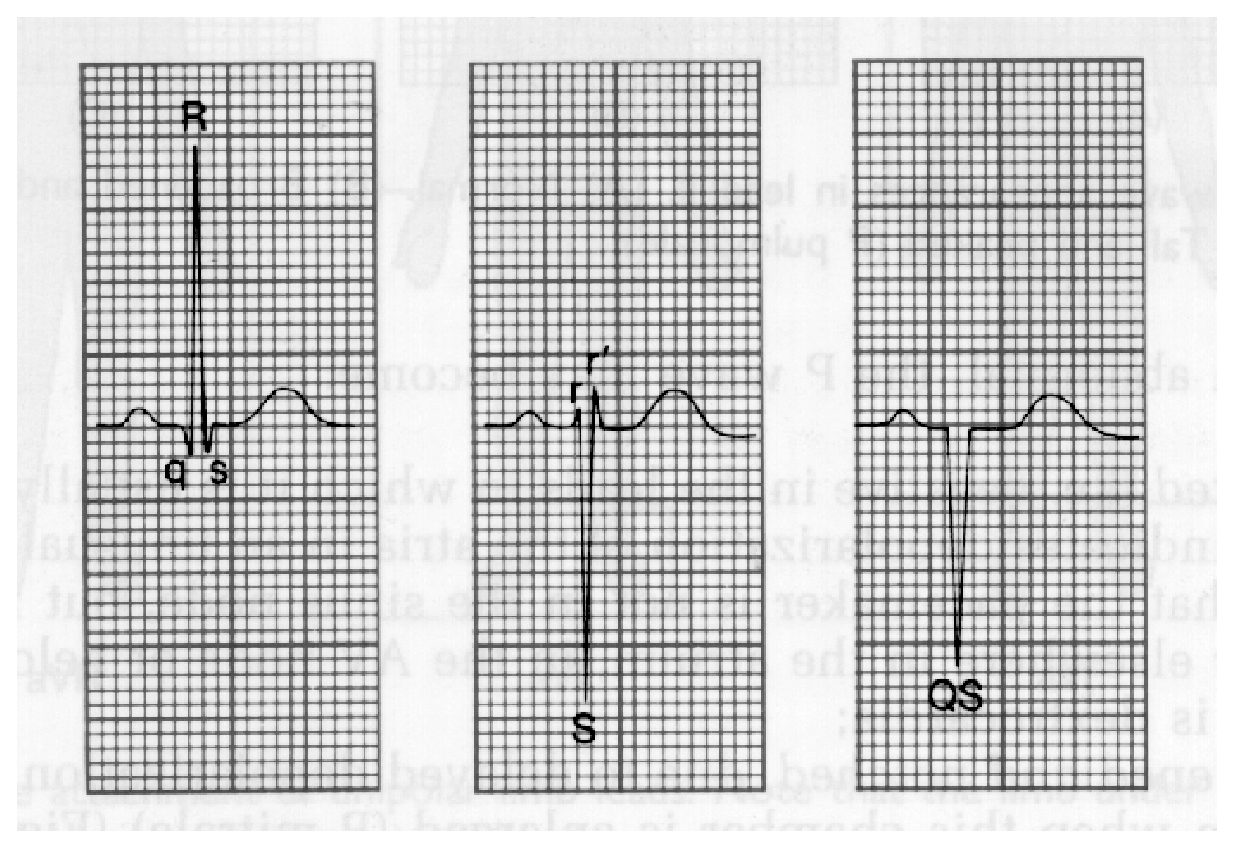
\epsfig{file=electrocardiology/epsfiles/qrs.eps,width=10cm}
 \caption[Variations in the QRS complex]{Variations in the QRS complex (see text)}
  \label{fig:qrs}
\end{figure}

\begin{itemize}
 \item the R wave is any positive(upward) deflection of QRS complex. If there
  is more than one R wave, the second is denoted R'; and R wave of small
  voltage may be denoted r; 
 \item a negative (downward) deflection preceding an R wave is termed Q;
 \item a negative (downward) deflection following an R wave is termed S
 \item if the ventricular complex is entirely negative (i.e. there is no R
  wave), the complex is termed QS.
\end{itemize}

The whole complex is often referred to as the QRS complex irrespective of
whether one or two of its components are absent.

Ventricular depolarisation starts in the middle of the left side of the septum
and spreads across to the right (phase 1 of ventricular depolarisation)
(Figure~\ref{fig:heartqrs}). Subsequently, the main free walls of the
ventricles are activated, the impulse spreading from within outwards and from
below upwards. Because of the dominating bulk of the left ventricle, the
direction of the vector of phase 2 is to the left and posteriorly. Finally,
the base of both ventricular walls and the interventricular septum are
depolarised. The appearances of the QRS in different leads can be largely
explained by the major vectors of these phases as seen in Figure
~\ref{fig:heartqrs}. In leads facing the left ventricular surface, there is a
small Q wave due to septal depolarisation and a large R wave due to left
ventricular depolarisation. On the right side of the heart, as seen by V1,
there is usually an r wave due to septal depolarisation and a large S wave
due to left ventricular forces directed away from the electrode.

\begin{figure}[htbp] \centering
  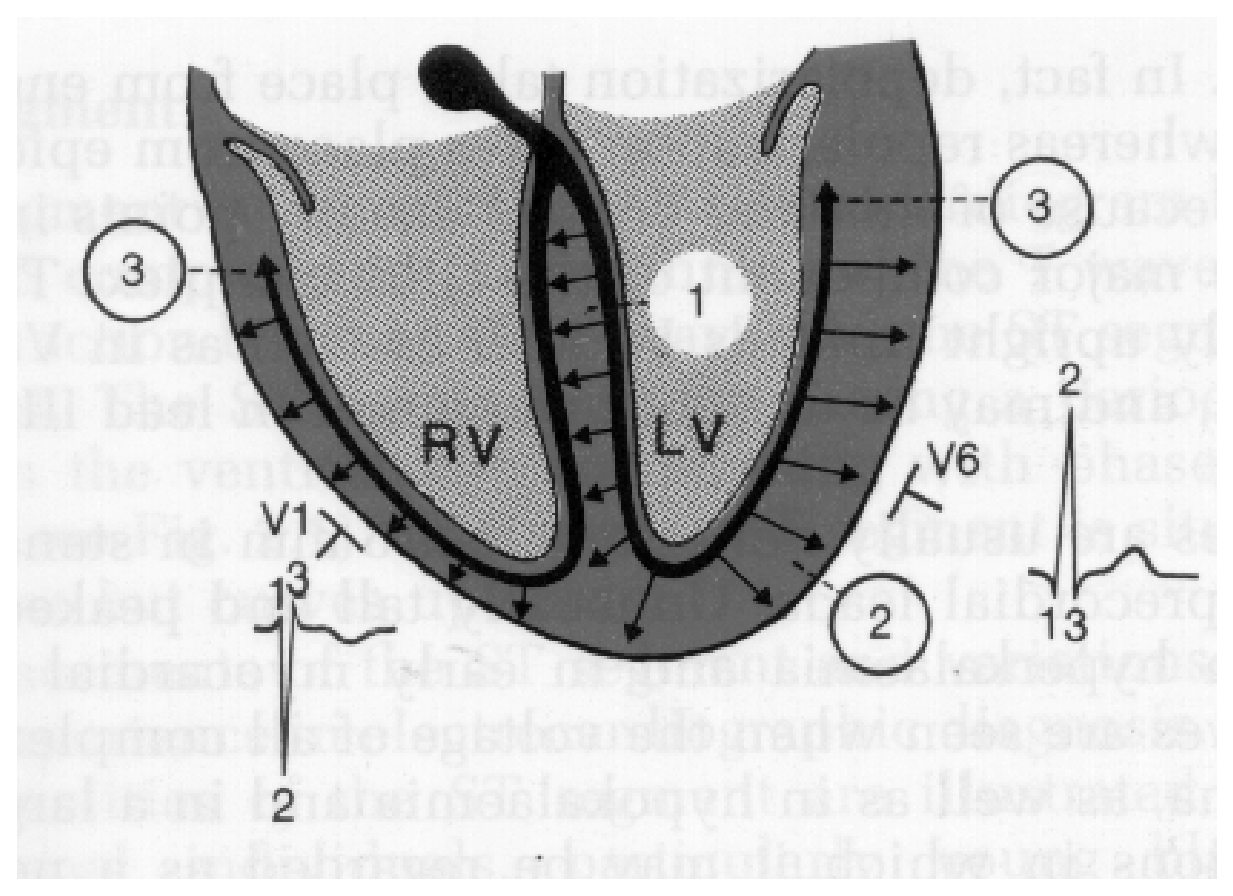
\epsfig{file=electrocardiology/epsfiles/heartqrs.eps,width=10cm}
 \caption[Genesis of QRS complex.]{Genesis of QRS complex. Note that the first phase, directed from
   left to right across the septum, produces a Q wave in $V6$ and an R wave in
   V1. The second phase, due mainly to depolarisation of the left ventricle
   from endocardium to epicardium, results in a tall R wave in V6 and a deep
   S wave in V1. Finally, depolarisation of the basal parts of the
   ventricles may produce a terminal S wave in V6 and a terminal R wave in V1}
  \label{fig:heartqrs}
\end{figure}

\paragraph{Pathological Q waves}
As mentioned, small, narrow Q waves are normally to be found in leads facing
the left ventricle, e.g. lead I, aVL, aVF, V5 and V6. These Q waves do not
normally exceed 2mm in depth, or 0.03s in width. It should be noted that QS
waves are normal in aVR, and are common in V1. Abnormally broad and deep Q
waves are often a feature of myocardial infarction. Q waves in lead III are
difficult to evaluate but can be ignored if there are no Q waves either in
lead II or in aVF, or if they do not exceed 0.03s. Usually a `normal' Q
wave in lead III diminishes or disappears on deep inspiration because of an
alteration in the position of the heart, whilst the `pathological' Q wave of
infarction persists.

The QRS complex should not exceed 0.10s duration, and usually is in the range
0.06-0.08s. Broad QRS complexes occur in bundle branch block, in ventricular
hypertrophy and in ventricular ectopic beats.

\subsubsection{The T Wave}

The T wave is due to depolarisation of the ventricles.  If repolarisation (the
T wave) occurred in the
same direction as depolarisation (the QRS complex) the T wave would be
directed in an opposite way to that of the QRS
complex. In fact, depolarisation takes place from endocardium to epicardium,
whereas repolarisation takes place from the epicardium to endocardium. Because
of this, the T wave usually points in the same direction as the major
component of the QRS complex. Thus, the T wave is normally upright in leads
I and II as well as in V3 to V6, is inverted in aVR, and may be
upright or inverted in lead III, aVL, aVF and V1 and V2.

The T waves are usually not taller than 5m in standard leads and 10mm in
praecordial leads. Unusually tall and peaked T waves may be seen in
hyperkalaemia and in early myocardial infarction. Flattened T waves are seen
when the voltage of all complexes is low, as in myxoedema, as well as in
hypokalaemia and in a large number of other conditions in which it may be
regarded as a non-specific abnormality. Slight T wave inversion is also often
non-specific , and may be due to such influences as hyperventilation, posture
and smoking. The most important casuses of T wave inversion are:
\begin{itemize}
\item myocardial ischaemia and infarction;
\item ventricular hypertrophy;
\item bundle branch block.
\end{itemize}

\subsubsection{The QT Interval}

The QT interval represents the total time from the onset of ventricular
depolarisation to the completion of repolarsation. It is measured from the
beginning of the Q wave (or R wave if there is no Q wave) to the end of the T
wave. Its duration varies with heart rate, becoming shorter as the heart rate
increases. In general, the QT interval at heart rates between 60 and 90 per
minute does not exceed in duration half the preceding PR interval. The
measurement of the QT interval is often difficult as the end of the T wave
cannot always be clearly identified, and the relationship between heart rate
and duration of the QT interval is a complex one. Tables are available in
textbooks of electrocardiography giving normal QT intervals. In practice, the
main importace of a prolonged QT interval is that it is associated with a risk
of ventricular tachycardias (particularly torsades de pointes), and sudden
death. A long QT is sometimes an inherited abnormality but may result from
such drugs as quinidine, procainamide, disopyramide, amiodarone and tricyclic
antidepressants.

\subsubsection{The ST Segment}
The ST segment is that part of the electrocardiogram between the end of the
QRS complex and beginning of the T wave. The point of junction between the S
wave and the ST segment is known as the J point. The ST segment occurs during
the period of unchanging polarity in the ventricles, corresponding with phase
2 of the action potential. The normal ST segment is situated on the
iso-electric line but curves upwards.

Displacements of the ST segment and variations in its shape are of great
importance in electrocardiographic diagnosis. ST segment elevation occurs because repolarisation of the injured tissue
occurs more rapidly than that of normal tissue and a potential gradient
exists.

\begin{tabular}{lp{10cm}}
ST elevation is caused by &-~ acute myocardial infarct (dead tissue with
injured tissue surrounding it)\\
 &-~pericarditis (inflammation of the pericardium\\
 &-~ventricular hypertrophy (enlarged ventricle)\\
 &-~myocardial ischaemia (detected as ST depression) (deficiency of blood to
part of the myocardium) can lead to myocardial infarcts\\
 &-~sinus tachycardia (fast heart beat, $>$100/ min, with its origin in the
 sinus node
\end{tabular}


\subsection{The U Wave}
The U wave is a broad, low-voltage wave present in most normal ECGs. Its cause
is unknown; it may become unusually prominent in hypokalaemia and with
digitalis therapy.

\subsection{Some Abnormal ECGs} 
%(see handouts 3-7)

Names of clinical conditions:
\begin{itemize}
\item Left ventricular hypertrophy %(figure missing)
\item Right ventricular hypertrophy \figref{fig:rvhypertrophy}
\item Left bundle branch block \figref{fig:leftbbb-ecg} 
(Purkinje fibres in the LV are interrupted \figref{fig:leftbbb} )
\item Right bundle branch block \figref{fig:rightbbb-ecg} 
(Purkinje fibres in the RV are interrupted \figref{fig:rightbbb} )
\item WPW (Wolff-Parkinson-White syndrome)
\end{itemize}

\begin{figure}[htbp] \centering
  \epsfig{file=electrocardiology/epsfiles/rvhypertrophy.eps,width=10cm}
  \caption[Right Ventricular Hypertrophy]{Right Ventricular Hypertrophy.  Note
    the deep S wave in lead VI and the tall R waves in lead V5 and V6}
  \label{fig:rvhypertrophy}
\end{figure}

\begin{figure}[htbp] \centering
  \epsfig{file=electrocardiology/epsfiles/leftbbb-ecg.eps,width=10cm}
  \caption[Left Bundle Branch Block ECG]{Left Bundle branch block ECG}
  \label{fig:leftbbb-ecg}
\end{figure}

\begin{figure}[htbp] \centering
  \epsfig{file=electrocardiology/epsfiles/leftbbb.eps,width=10cm}
  \caption[Left Bundle Branch Block]{Left Bundle Branch Block.  The inital
    vector is abnormal in being from right to left in the septum, thus
    producing an initial R wave in V6 and a Q wave in V1}
  \label{fig:leftbbb}
\end{figure}

\begin{figure}[htbp] \centering
  \epsfig{file=electrocardiology/epsfiles/rightbbb-ecg.eps,width=10cm}
  \caption[Right Bundle Branch Block ECG]{Right Bundle branch block ECG}
  \label{fig:rightbbb-ecg}
\end{figure}

\begin{figure}[htbp] \centering
  \epsfig{file=electrocardiology/epsfiles/rightbbb.eps,width=10cm}
  \caption[Right Bundle Branch Block]{Right Bundle Branch Block.  The septum
    is depolarised normally from left to right and hence a small Q is
    present in left ventricular leads and a small R in right ventricular
    leads.  Left ventricular depolarisation causes an S wave in V1 and an R
    wave in V6.  Late depolarisation of the right ventricle results in a
    prominent R' wave in V1 and broad S wave in V6}
  \label{fig:rightbbb}
\end{figure}

What can happen?

\noindent Ventricular Tachycardia (VT) - caused by slow conduction, or
presence of an infarct. This can lead to Ventricular Fibrillation (VF) where
there is no discernable pattern.  Death quickly follows if this is not
treated. %see ER!!! 

\begin{tabular}{lcp{13cm}}
Treatment &-&external defibrillation\\
          &-&internal defibrillator (implantable, onto heart, lasts
          about 4 years)
\end{tabular}

The strengths and limitations of the various treatments for ventricular
tachyarrhythmias is given in \figref{fig:tachy-arryth}.

\begin{figure}[htbp] \centering
  \epsfig{file=electrocardiology/epsfiles/tachy-arryth.eps,width=10cm}
  \caption[Ventricular Tachyarrhythmia Management]{The strenths and
    weakenss associated with the various Ventricular Tachyarrhythmia
    management options}
  \label{fig:tachy-arryth}
\end{figure}

\section{Usefulness of ECG}

The ECG is used to determine what is happening to the heart (how it is
performing, etc.).  This is an ``inverse'' problem (inverse problems are very
difficult to solve) - i.e. given this set of ECGs, what is the heart doing. (
The `forward' problem would be, given that the heart is doing this (i.e. has a
given electrical activation pattern), what is the corresponding ECG - this
would be far easier to solve).

The `inverse' problem is solved largely by pattern recognition.  There are
books of ECGs which illustrate different problems - just find the right ECG
(durations of different waves, heights, etc. give clues to possible
irregularities).There is a standard set of steps to reading an ECG \figref{fig:ecg-interpretation}.

\begin{figure}[htbp] \centering
  \epsfig{file=electrocardiology/epsfiles/ecg-interpretation.eps,width=10cm}
  \caption[ECG Interpretation]{A procedure for interpreting ECGs}
  \label{fig:ecg-interpretation}
\end{figure}

In later sections we will consider the underlying mathematical theory behind
the ECG.  We now discuss a more generalised approach to ECG monitoring -
namely body surface potential mapping.

\section{Body Surface Potential Mapping (BSPM)}
ECGs do well, but do not provide the whole answer. e.g. they can tell WPW is
present, but not where the accessory pathway is; they can (sometimes) detect
infarcts and ischaemic regions, but not identify where these regions are. A
famous example is the case of Sir Richard Hadlee \figref{fig:hadley} 
who had open chest surgery to
correct is WPW problem (which was identified with an ECG but could not be
localised without more detailed mapping).

\begin{figure}[htbp] \centering
  \epsfig{file=electrocardiology/epsfiles/hadley.eps,width=10cm}
  \caption[Sir Richard Hadlee]{The newspaper article
    mentioning Sir Richard Hadlee's WPW problem}
  \label{fig:hadley}
\end{figure}

BSPM was brought about by the development of full chest lead systems
to sample electrical activity at a relatively large number of sites. It began
in the early 60s (?) and is not usually used clinically, however, those places
that use it get good results.  The problems with BSPM are that
it can be more time consuming, there are no standard lead sets, it requires more
setup time (there is a need to store and view a great deal of data), and an
ECG provides a lot of information available on BSPM, suggesting that the extra
work is not worth the effort. 

Two examples of BSPM systems are given in \figref{fig:body-suit2}, 
\figref{fig:body-suit},  \figref{fig:body-suit-utah} and 
\figref{fig:body-suit2-utah}. \figref{fig:body-suit2} and  
\figref{fig:body-suit} are of the system used in Hobart, Australia and contain a large
number of active (dry) electrodes that are embedded between 2 layers of
neoprene. This suit can be applied quickly and a recording obtained in about
the same time as that needed for a standard 12 lead ECG.  The person
standing in \figref{fig:body-suit2} often uses this system in acute patients
(in the ER room for instance) in preference to a 12 lead ECG.  The other 2
figures, \figref{fig:body-suit-utah} and  
\figref{fig:body-suit2-utah} are from a system in use in Salt Lake City, Utah.
Strips of electrodes are placed over part of the torso at pre-specified
locations. Each electrode is full with a conducting gel and contains a
surround of adhesive, so they stick to the skin.  This 32 lead system was
obtain  from looking at maps recorded with 120
leads and doing a statistical decomposition and evalue analysis.  It was found
that an ECG provides approximately 90\% of the information available and 32
leads yield approximately 98\%.

\begin{figure}[htbp] \centering
  \epsfig{file=electrocardiology/epsfiles/body-suit2.eps,width=10cm}
  \caption[Hobart body surface mapping system]{Hobart Body surface mapping system}
  \label{fig:body-suit2}
\end{figure}

\begin{figure}[htbp] \centering
  \epsfig{file=electrocardiology/epsfiles/body-suit.eps,width=10cm}
  \caption[Hobart body surface suit]{Hobart Body surface suit}
  \label{fig:body-suit}
\end{figure}

\begin{figure}[htbp] \centering
  \epsfig{file=electrocardiology/epsfiles/body-suit-utah.eps,width=10cm}
  \caption[Utah body surface mapping suit]{Utah body surface mapping suit}
  \label{fig:body-suit-utah}
\end{figure}

\begin{figure}[htbp] \centering
  \epsfig{file=electrocardiology/epsfiles/body-suit2-utah.eps,width=10cm}
  \caption[Utah body surface mapping suit - another view]{Utah body surface
    mapping suit- another view}
  \label{fig:body-suit2-utah}
\end{figure}

Schematics of other lead systems are given in \figref{fig:vcg-bspm} and
\figref{fig:bspm-leads}. The first of these shows the location of the standard
ECG leads in a uniform electrode array.  The other figure shows 2 lead sets
that have been proposed which are said to yield almost all the information of
the uniform array. 

\begin{figure}[htbp] \centering
  \epsfig{file=electrocardiology/epsfiles/vcg-bspm.eps,width=10cm}
  \caption[Schematic of uniform lead set]{Comparison of torso electrode
    locations for vectorcardiography (F), for standard electrocardiography (S)
    and for body surface potential mapping.  The vertical lines marks the
    sternum.}
  \label{fig:vcg-bspm}
\end{figure}

\begin{figure}[htbp] \centering
  \epsfig{file=electrocardiology/epsfiles/bspm-leads.eps,width=10cm}
  \caption[Various BSPM electrode locations]{Utah body surface
    mapping suit- another view. Electrocardiographics lead sets proposed by Barr
    (A- Duke) and Lux (B- Salt Lake City) }
  \label{fig:bspm-leads}
\end{figure}

Implantable defibrillators are being widely used
instead of fixing the problem. There is a lack of good modelling and diagnostic
cabability. However, it is our view that with good modelling and new imaging techniques, and the
cooperation of clinical staff, a great deal of progress can be made. We
currently have our own BSPM system.

\subsection{BSPM at Halifax, Canada}
We present in this section real BSPM maps recorded from patients suffering
from WPW in Dalhousie University, Halifax, Canada.  
The emphasis on this system is due to the
availability of the measured maps.  As mentioned above, WPW is a condition in
which an accesory pathway exists between the atria and ventricles. Although this does not affect a large proportion of the population it is a
situation in which BSPM has been very successful since the site of the
accessory pathway can, in most cases, be determined before inserting a
catheter for ablation (5-10 years ago open heart surgery was required).
 It is
relatively easy to fix (just cut/ablate the tissue involved) once the region
has been localised.  It is also fairly easy to detect on an ECG
\figref{fig:deltawave-ecg}, \figref{fig:deltawave} but it cannot be localised
using a standard ECG.

\begin{tabular}{lcp{13cm}}
Cause & - & breakdown of ``insulation'' between atria and ventricles.  Ventricles
are being stimulated from above and below - loss of pumping efficiency.\\
Cure & - & find accessory pathway and ablate (i.e. burn part of the tissue with a
catheter - this is inserted in the leg).
\end{tabular}

\begin{figure}[htbp] \centering
  \epsfig{file=electrocardiology/epsfiles/deltawave-ecg.eps,width=10cm}
  \caption[WPW ECG]{Part of an ECG of a WPW condition.  At slower rates
    (bottom) a delta wave is more prominent that it is at higher rates}
  \label{fig:deltawave-ecg}
\end{figure}

 \begin{figure}[htbp] \centering
  \epsfig{file=electrocardiology/epsfiles/deltawave.eps,width=10cm}
  \caption[Delta wave]{Scehmatic representation of ECG features of the WPW
    patten.}
  \label{fig:deltawave}
\end{figure}

Figure \figref{fig:halifax-mesh} illustrates the electrode locations used in
the Halifax system (black dots - left hand side is the front).  Recordings
from a healthy male are given in \figref{fig:hal-leads-norm-front} (front) and
\figref{fig:hal-leads-norm-back} (back).  Note that some of the leads given no
recording, so are discard in the final analysis.  The position of the standard
V1 and V2 leads are marked.  The recordings given are based on averages of 10
seconds of recordings.

 \begin{figure}[htbp] \centering
  \epsfig{file=electrocardiology/epsfiles/halifax-mesh.eps,width=10cm}
 \caption[Lead location of Halifax BSPM system]{The location of the electrodes
   used in the BSPM system at Halifax.  The left hand side represents the
   front, and electrodes are denoted using black dots}
  \label{fig:halifax-mesh}
\end{figure}

 \begin{figure}[htbp] \centering
  \epsfig{file=electrocardiology/epsfiles/hal-leads-norm-front.eps,width=10cm}
 \caption[Normal BSPM recording]{The front recordings from a normal male 
 using the
   Halifax BSPM system (10 seconds of recordings that have been averaged.  Note that some leads give no recording and are
   therefore discarded from further analysis.  The location of the leads V1
   and V2 have been marked.  The left hand code is the code as per the NY
   Heart Association handbook}
  \label{fig:hal-leads-norm-front}
\end{figure}

 \begin{figure}[htbp] \centering
  \epsfig{file=electrocardiology/epsfiles/hal-leads-norm-back.eps,width=10cm}
 \caption[Normal BSPM recording - back]{The back recordings from a normal
   male using the Halifax BSPM system }
  \label{fig:hal-leads-norm-back}
\end{figure}

Fiducial markers (start and end of QRS etc) are then obtained by looking at
the Frank VectorCardiograph leads \figref{fig:hal-vcg-normal} (i.e. looking at the difference in potential
across the body, front-back of the body and up/down on the body). 

 \begin{figure}[htbp] \centering
  \epsfig{file=electrocardiology/epsfiles/hal-vcg-normal.eps,width=10cm}
 \caption[Normal VCG from Halifax system]{ The VCG used to determine the
   Fiducial markers. PON is the start of the P wave (in ms) POFF the end of
   the P wave, RON and ROFF the equivalent times for the R wave and TOFF is
   end of the T wave. }
  \label{fig:hal-vcg-normal}
\end{figure}

After the fiducial markers have been identified, the data is interpolated to
present the body surface potential maps seen in
\figref{fig:hal-bspm-normala} to \figref{fig:hal-bspm-normalc}. These figures
are maps of the contours of potential at 10 ms intervals.  The first maps are
simply just noise (since these are before activation) and the times
corresponding to the fiducial markers (RON and ROFF) are identified. RPK
corresonds to the peak of the QRS.  The location of the extrema are also
plotted and negative potentials are given in dashed contour lines. 

 \begin{figure}[htbp] \centering
  \epsfig{file=electrocardiology/epsfiles/hal-bspm-normala.eps,width=10cm}
 \caption[Normal BSPM maps (a)]{Isopotential lines for a normal patient at
 10 ms intervals.  The first maps are
simply just noise since these are before activation and the times
corresponding to the fiducial markers RON and ROFF are identified. RPK
corresonds to the peak of the QRS.  The location of the extrema are also
plotted and negative potentials are given in dashed contour lines.}
  \label{fig:hal-bspm-normala}
\end{figure}

\begin{figure}[htbp] \centering
  \epsfig{file=electrocardiology/epsfiles/hal-bspm-normalb.eps,width=10cm}
 \caption[Normal BSPM maps (b)]{Normal BSPM maps (b) }
  \label{fig:hal-bspm-normalb}
\end{figure}

\begin{figure}[htbp] \centering
  \epsfig{file=electrocardiology/epsfiles/hal-bspm-normalc.eps,width=10cm}
 \caption[Normal BSPM maps (c)]{Normal BSPM maps (c) }
  \label{fig:hal-bspm-normalc}
\end{figure}


\subsubsection{Things to look for}
-positions of maximum and minimum and how these move (and locations of
``zero'' line).
 
\begin{tabular}{lcl}
-before RONN  & - & noise\\
-early R & - & septal activation
\end{tabular}

As activation reaches the apex, the negative region moves over the right
shoulder.

As activation moves up (``deflection'' pointing outward?) there is widespread
left ventricular and right ventricular epicardial breakthrough.  The pattern
can become complicated and variable.  Usually the maximum moves slowly around
the back \figref{fig:bspm-max-min}.

\begin{figure}[htbp] \centering
  \epsfig{file=electrocardiology/epsfiles/bspm-max-min.eps,width=10cm}
  \caption[BSPM max-min trajectories]{Trajectory maps depicting postion of the
    maxima (top) and minima (bottom) during the QRS copmlex.  The left half of
    each map represents the front of the torso.  Selected instants, labelled
    A through G, are shown.  During the end of the QRS complex, three
    variations (1, 2, and 3) are observed}
  \label{fig:bspm-max-min}
\end{figure}


\subsection{Abnormal Maps}
To help in the interpretion of BSPM from WPW patients, Dalhousie University
 has a model of a human heart (anatomically accurate) in a
model of a torso.  It had a rule-based activation process (cellular-automata,
cells 1mm$^{3}$), and each cell had a set of rules about when it will become
activated and for how long.   This determines epicardial potentials and then
a BEM torso model was used to solve for torso potentials (homogenous torso).

They ran a number of simulations for a number of pre-excitation slices (\figref{fig:hal-heart-model}) and calculated the body surface potentials for each preexcitation
(most prominent differences).  The results of each of these simulations are 
shown in \figref{fig:hal-bspm-template}. The locations
  of the extrema and respective regions of positivity and negativity are used
  to distinguish each map.  These templates are used to help localise the
  accesory pathway.  A patient suffering from WPW (diagnosed from a standard
 ECG) will have a body surface map taken.  This is then compared to the
 templates and the accessory pathway site estimated.  The patient will then
 undergo catheter surgery to localise the  site (starting at the estimated
 site).  In almost all cases, the estimated site corresponds to the site that
 is ablated.  Examples of real maps, and the actual ablation site
 are given in \figref{fig:hal-bspm-wpw1} to  
\figref{fig:hal-bspm-wpw6}.  Note how well these sites are predicted using
  the templates. 

\begin{figure}[htbp] \centering
  \epsfig{file=electrocardiology/epsfiles/hal-heart-model.eps,width=10cm}
  \caption[Halifax Heart Model]{Top 20 Bassal sections of the ventricular
    haeart model used at Halifax.  There were 14 preexcitation sites.  The
    sections, which are 1 mm apart, are represented by smoothed contour lines
    to achieve a better rendering of the shape.  Note that the ventricular
    structure is rid of all non-excitable tissues in the atrioventricular ring.
    RV = right ventricle; LV = left ventricle; PA = pulmonary artery; AP=
    anterior parseptal; AS - anterior septal; A - anterior, AL =
    anteropateral; L=lateral; PL = posterolateral; P = posterior; PP =
    posterior paraseptal }
  \label{fig:hal-heart-model}
\end{figure}

\begin{figure}[htbp] \centering
  \epsfig{file=electrocardiology/epsfiles/hal-bspm-template.eps,width=8.5cm}
  \caption[Simulated WPW maps]{The simulated BSPMS at 40ms after the onset of
    stimulation which was individualy applied at the 14 preexcitation sites
    shown in  \figref{fig:hal-heart-model}.  The right and left borders of each
      map both correspond to the right mid-axillary line; the lower border
      corresponds to the waist.  Isopotential lines progress logarithmically
      and the principal extrema have their amplitudes marked in microvolts }
  \label{fig:hal-bspm-template}
\end{figure}

\begin{figure}[htbp] \centering
  \epsfig{file=electrocardiology/epsfiles/hal-bspm-wpw1.eps,width=10cm}
  \caption[Real BSPM WPW map (a)]{A real BSPM from a WPW patient.  The accesory
    pathway is at LAL which is predicted using the template }
  \label{fig:hal-bspm-wpw1}
\end{figure}

\begin{figure}[htbp] \centering
  \epsfig{file=electrocardiology/epsfiles/hal-bspm-wpw2.eps,width=10cm}
  \caption[Real BSPM WPW map (b)]{Real WPW map (b) }
  \label{fig:hal-bspm-wpw2}
\end{figure}

\begin{figure}[htbp] \centering
  \epsfig{file=electrocardiology/epsfiles/hal-bspm-wpw3.eps,width=10cm}
  \caption[Real BSPM WPW map (c)]{Real WPW map (c) }
  \label{fig:hal-bspm-wpw3}
\end{figure}

\begin{figure}[htbp] \centering
  \epsfig{file=electrocardiology/epsfiles/hal-bspm-wpw4.eps,width=10cm}
  \caption[Real BSPM WPW map (d)]{Real WPW map (d). The best template match was
    LAL and LL. }
  \label{fig:hal-bspm-wpw4}
\end{figure}

\begin{figure}[htbp] \centering
  \epsfig{file=electrocardiology/epsfiles/hal-bspm-wpw5.eps,width=10cm}
  \caption[Real BSPM WPW map (e)]{Real WPW map (e).  The best template match was
   RAS and LPP}
  \label{fig:hal-bspm-wpw5}
\end{figure}

\begin{figure}[htbp] \centering
  \epsfig{file=electrocardiology/epsfiles/hal-bspm-wpw6.eps,width=10cm}
  \caption[Real BSPM WPW map (f)]{Real WPW map (f).  There were 2 accesory
    pathways  at LAP and LPP }
  \label{fig:hal-bspm-wpw6}
\end{figure}

\section{The Forward and Inverse Problems of Electrocardiography}
\subsection{Introduction}
\enlargethispage{-\baselineskip}
\enlargethispage{-\baselineskip}
\enlargethispage{-\baselineskip}
The goal of non-invasive electrical imaging of the heart is to
quantitatively reconstruct information about the electrical activity
of the heart from densely sampled thoracic ECG signals. 

Quantitative interpretation of the densely sampled data in terms of the
underlying cardiac electrical activity is an inverse problem, and various
mathematical algorithms have been developed over the years in an attempt to
solve this electrical imaging problem 
e.g. \cite{barr:1978,gulrajani:1984,martin:1975,oster:1992}. Unless the problem is
posed in a particular manner this inverse problem is not uniquely determined
i.e. there exist multiple cardiac electrical generator configurations that can
give rise to the same thoracic ECG measurements. This non-uniqueness has
hampered attempts at solving the inverse problem.  Early approaches to the
inverse problem overcame the non-uniqueness by modelling the heart as a
combination of a small number of fixed or moving dipoles.  It has been
recognised that posing the problem in terms of trying to reconstruct
epicardial potentials from the body surface potential recordings is uniquely
determined. However, the reconstruction of epicardial potentials is ill-posed.
This means that in the presence of noise (which always exists) a solution to
the inverse problem produces a result which may bear no resemblance to that of
the true electrical generator.  The emergence of a general theory for such
ill-posed problems \cite{tikhonov:1977} and the introduction of the ideas
behind constraining the mathematical solutions has resulted in the large
number of variants of the inverse algorithms in existence today in the
electrical imaging area.  However, since they are based on a generic approach,
most of the modern algorithms fail to incorporate the underlying physiological
processes governing the generation of the body surface potentials (namely an
evolving wave of activation).  Most of these algorithms also do not impose the
constraints in a mathematically correct fashion
\cite{greensite:1998b,greensite:1998}.

\subsection*{A New Approach}

Another approach to the inverse problem is to pose the problem in terms of the
underlying activation sequence \cite{huiskamp:1988}. This has significant advantages
over the epicardial potential problem formulation, not least in that it deals
directly with the underlying physiological process responsible for generating the
body surface potentials. However, it introduces additionally difficulties in the
modelling process (for instance the need to accurately model the entire heart instead
of just modelling the epicardial surface).  Because of this, and partly because of
the fact that an appropriate algorithm for such a problem formulation had
previously not been devised, this approach has not found much favour.
However, a powerful new algorithm, based on this activation imaging approach
has recently emerged \cite{greensite:1998b,huiskamp:1997}.

Both the epicardial and activation source formulations mentioned above have
been recognised for twenty to thirty years but as of yet no clinically
acceptable imaging techniques have resulted. The two major reasons for this
are
\begin{enumerate}
\item Previously available mathematical methodologies for computation of the
  sources were not powerful enough.
\item Adequate procedures for verification of the accuracy of the images were
  not employed.
\end{enumerate}
For each of the two source formulations there are now powerful imaging
algorithms that have not previously been available, 
e.g. \cite{greensite:1998b,greensite:1998,huiskamp:1997}. There are also
sufficient modelling techniques now available that when combined with these new
algorithms should make it possible to produce myocardial electrical source images of
sufficient stability and accuracy to be a useful adjunct in the clinical
assessment of the heart. However, these new algorthims need to be quantitatively
validated before teh clinical worth can be properly assessed.

In order to quantitatively validate the performance of the inverse procedures, one
needs to compare any mathematical results against experimentally-obtained 
\emph{invivo} data, in particular simultaneously recorded densely sampled body
surface and cardiac potentials.  This has rarely been attempted -- rather the
worth of various inverse procedures has often been judged by examining the
performance on simulated data or in \emph{in vitro} torso tank experiments.  As
far as is known, only two sets of \emph{invivo} data have ever been collected, one
in a chimpanzee \cite{spach:1979} (in which no inverse solution was attempted)
and one in a dog \cite{barr:1978}.  Neither set is currently available.  Data
from \emph{in vitro} experiments from perfused canine hearts in a homogeneous
cylindrical tank have been collected by Taccardi \emph{et. al.} and are in use by that
group and others \cite{oster:1992,oster:1997,oster:1998}.

We are currently performing experiments on pigs to provide the necessary \emph{invivo}
data to validate the new inverse procedures.  We present here the details of
the underlying theory behind the electrical imaging process and the porcine
model development.  We also illustrate how the procedure is to be applied in
practice by producing an inversely-reconstructed cardiac surface activation
map from simulated data.  
%A companion paper will focus on the experimental
%procedure and the quantitative validation of this inverse reconstruction from
%experimental \emph{invivo} data.


%%%%%%%%%%%%%%%%%%%%%%%%%%%%%%%%%%%%%%%%%%%%%%%%%%%%%%%%%%%%%%%%%%%%%%%%%%%%%%%
%% Theory
%%%%%%%%%%%%%%%%%%%%%%%%%%%%%%%%%%%%%%%%%%%%%%%%%%%%%%%%%%%%%%%%%%%%%%%%%%%%%%%

\section{Theory}
\enlargethispage{\baselineskip}
The basic activation inverse algorithm is presented in Huiskamp and 
Greensite \cite{huiskamp:1997}.
The procedure revolves around the identification of the critical
points and times of the surface activation function (i.e. epi- and
endocardial breakthrough/termination points and times) via the use of
a modified MUSIC algorithm.  To use this method on a given
individual/animal requires the construction of an appropriate transfer
function or mapping from the activation sequence to body surface
potentials.

The proof of the activation imaging algorithm \cite{greensite:1998b} uses
source field relationships given in \cite{yamashita:1985}.  These
relationships employ a Green's function that takes into account the anisotropy
of the myocardium.  While the new imaging algorithm proved from these
relationships is completely general, the initial use of it has been restricted
to using the so-called double layer transfer matrices, which assume a
homogeneous and
isotropic heart muscle.  The traditional construction of such a double-layer
transfer matrix begins with the assumption of myocardial homogeneity and
isotropy and the use of equations defining the potential due to a dipole in
freespace \cite{cuppen:1984}. We prefer to investigate the transfer matrix
construction from a boundary value problem point of view (e.g. from solving
the bidomain equations) which avoids explicit reference to dipoles, and makes
more explicit the anisotropic/isotropic distinction.  This approach also
generalises some of the identities presented in \cite{yamashita:1985}.

\subsection{Transfer Matrices From A Boundary Value Problem Point of View}
Let $D_{H}$ be the domain of the heart, $S_{H}=$ $\partial D_{H}$ (closed),
$\phi _{i}$ the intracellular potential,
$\phi _{e}$ the extracellular potential,
$\phi _{m}$ the transmembrane potential ($=$ $\phi _{i}-\phi _{e}$ ),
$\phi $ the torso potential outside $D_{H}$ and
$\overline{G_{i}}$ and $\overline{G_{e}}$ the intracellular and
extracellular conductivity tensors.

From bidomain theory we have inside $D_{H}$

\begin{equation}
\nabla \cdot ([\overline{G_{i}}+\overline{G_{e}}]\nabla \phi _{e})=-\nabla
\cdot (\overline{G_{i}}\nabla \phi _{m})  \label{current_cons}
\end{equation}

This is a Poisson equation for $\phi _{e}$ in which the source term is $%
-\nabla \cdot (\overline{G_{i}}\nabla \phi _{m}).$

One can solve this partial differential equation using a weighted residuals approach. 
Let $w$ be a (as-yet-unspecified) weighting function. Then, from weighted residuals

\begin{equation}
0=\int_{D_{H}}\nabla \cdot ([\overline{G_{i}}+\overline{G_{e}}]\nabla \phi
_{e})wd\Omega +\int_{D_{H}}\nabla \cdot (\overline{G_{i}}\nabla \phi
_{m})wd\Omega  \label{weighted_resid}
\end{equation}

Using Green's theorem we get
%%
\begin{equation}
0=\int_{S_{H}}w[\overline{G_{i}}+\overline{G_{e}}]\nabla \phi _{e}\cdot
ndS-\int_{D_{H}}[\overline{G_{i}}+\overline{G_{e}}]\nabla \phi _{e}\cdot
\nabla wd\Omega +\int_{D_{H}}\{\nabla \cdot (\overline{G_{i}}\nabla \phi
_{m})\}wd\Omega  \label{Start_fem_eqtn}
\end{equation}
where $n$ is the unit outward normal.

Applying Green's theorem again, one gets 
\begin{multline}
        0 =\int_{S_{H}}w[\overline{G_{i}}+\overline{G_{e}}]\nabla \phi _{e}\cdot
        ndS-\int_{S_{H}}\phi _{e}[\overline{G_{i}}+\overline{G_{e}}]\nabla w\cdot
        ndS  \\
        + \int_{D_{H}}\nabla \cdot ([\overline{G_{i}}+\overline{G_{e}}]\nabla w)
        \phi_{e}d\Omega +\int_{D_{H}}\nabla \cdot (\overline{G_{i}}\nabla 
        \phi_{m})wd\Omega   
        \label{Start_bem_eqtn}
\end{multline}

This is the standard boundary integral equation for Poisson's equation with
a general source term. For the special case of the source being given by $-%
\nabla \cdot (\overline{G_{i}}\nabla \phi _{m})$ we can apply a similar
procedure to that above on this term i.e. 
\begin{eqnarray}
\int_{D_{H}}\nabla \cdot (\overline{G_{i}}\nabla \phi _{m})wd\Omega 
        &=&\int_{S_{H}}w\overline{G_{i}}\nabla \phi _{m}\cdot ndS-\int_{D_{H}}
        \overline{G_{i}}\nabla \phi _{m}\cdot \nabla wd\Omega   \nonumber \\
        &=&\int_{S_{H}}w\overline{G_{i}}\nabla \phi _{m}\cdot ndS 
                -\int_{S_{H}} \phi_{m}\overline{G_{i}}\nabla w\cdot ndS  \nonumber \\
                && \quad + \int_{D_{H}}\nabla \cdot (\overline{G_{i}}\nabla w)\phi _{m}d\Omega 
        \label{source_term}
\end{eqnarray}

Inserting \eqnref{source_term} into \eqnref{Start_bem_eqtn} we get

\begin{eqnarray}
        0 &=&\int_{S_{H}}w[\overline{G_{i}}+\overline{G_{e}}]\nabla \phi _{e}\cdot ndS
                -\int_{S_{H}}\phi _{e}[\overline{G_{i}}+\overline{G_{e}}]\nabla w\cdot ndS 
                          \nonumber \\
                && \quad
                        + \int_{D_{H}}\nabla \cdot ([\overline{G_{i}}+\overline{G_{e}}]\nabla w)
                        \phi_{e}d\Omega +\int_{S_{H}}w\overline{G_{i}}\nabla \phi _{m}\cdot ndS 
                        \nonumber \\
                && \quad 
                        - \int_{S_{H}}\phi _{m}\overline{G_{i}}\nabla w\cdot ndS+\int_{D_{H}}\nabla
                        \cdot (\overline{G_{i}}\nabla w)\phi _{m}d\Omega   
        \label{BIE eqtn}
\end{eqnarray}

which is a generalisation of Equation 31 of \cite{yamashita:1985}.

This \eqnref{BIE eqtn} is general - no assumptions (apart from
differentiability and integrability) have been made on $w,\overline{G_{i}}\ $%
or $\overline{G_{e}}$. In \cite{yamashita:1985}, they
assumed that $w$ was a Green's function satisfying

\begin{equation}
\nabla \cdot ([\overline{G_{i}}+\overline{G_{e}}]\nabla w)+\delta (P)=0
\label{Greens_fn}
\end{equation}

and 
\begin{equation}
\lbrack \overline{G_{i}}+\overline{G_{e}}]\nabla w\cdot n=0\text{ on }S_{B}
\text{ }  \label{no_flux}
\end{equation}

where $\delta (P)$ is the Dirac delta distribution centred at a point $P$ and
$S_{B}$ is the surface of the torso.  This resulted in the removal of the
first volume integral in \eqnref{BIE eqtn}.

In practice, such a Green's function for the heart cannot be found
analytically, since both $\overline{G_{i}}$ and $\overline{G_{e}}$ 
are in general anisotropic and inhomogeneous.
If one assumes that they are homogeneous then both conductivity tensors can be
represented by a constant $3\times 3$ matrix, which is diagonal in the coordinate
system defined by the myocardial fibres and sheets. The fibre/sheet orientation in
the heart is very complex, which means that it is not possible in practice to solve
\eqnref{Greens_fn} analytically even under the assumption of homogeneity, or
even equal anisotropy ratios (i.e. $G_{i}=kG_{e}$ where $k$ is a constant).
This is true irrespective of whether we strive for a proper Green's function
(i.e. impose \eqnref{no_flux}) or merely look for a freespace Green's
function (also known as a fundamental solution) which is a solution of
\eqnref{Greens_fn} with zero boundary conditions at infinity (i.e. the no-flux
condition on $S_{B}$ is ignored).

If one assumes further that the domain is isotropic in both the extra and intracellular
domains, then one can apply a standard boundary element procedure to 
\eqnref{BIE eqtn}. For this we take $w$ to be the freespace Green's function 
i.e. a solution of
\begin{equation}
\nabla \cdot ([(1+k)G_{e}]\nabla w)+\delta (P)=0
\label{Fundamental_soln_eqtn}
\end{equation}

subject to zero boundary conditions at infinity. In three-dimensions, the
solution of this equation is
\begin{equation}
w=\frac{1}{4\pi (1+k)G_{e}R}  \label{Fundamental_soln}
\end{equation}

where $R$ is the distance measured from $P$. 

With $w$ defined as above, we get, for $P$ inside $D_{H}$

\begin{eqnarray}
\int_{D_{H}}\nabla \cdot ([\overline{G_{i}}+\overline{G_{e}}]\nabla w)\phi
_{e}d\Omega  &=&\int_{D_{H}}\nabla \cdot ([(1+k)G_{e}]\nabla w)\phi
_{e}d\Omega   \nonumber \\
&=&-\phi _{e}(P)  \label{Volume_int_phie}
\end{eqnarray}

and 
\begin{eqnarray}
\int_{D_{H}}\nabla \cdot (\overline{G_{i}}\nabla w)\phi _{m}d\Omega 
&=&\int_{D_{H}}\nabla \cdot (kG_{e}\nabla w)\phi _{m}d\Omega   \nonumber \\
&=&-\frac{k}{k+1}\phi _{m}(P)  \label{Volume_int_phim}
\end{eqnarray}

So \eqnref{BIE eqtn} becomes 
\begin{eqnarray}
0 &=&\int_{S_{H}}w(1+k)G_{e}\nabla \phi _{e}\cdot ndS-\int_{S_{H}}
        \phi_{e}(1+k)G_{e}\nabla w\cdot ndS-\phi _{e}(P)  \nonumber \\
        &&\quad +\int_{S_{H}}wkG_{e}\nabla \phi _{m}\cdot ndS-\int_{S_{H}}
        \phi_{m}kG_{e}\nabla w\cdot ndS-\frac{k}{k+1}\phi _{m}(P)
        \label{BIE_eqtn_p_inside}
\end{eqnarray}

The equation of more interest is the case for when $P\in S_{H}$ (i.e. $P$ is
on the boundary of the domain). To derive this equation, consider $P$ at a
smooth point on the
boundary of $D_{H}$ and construct a hemispherical region of radius $%
\varepsilon $ centred at $P$ . Let $D_{H}^{^{\prime }}$ be the extended
region (i.e. $D_{H}$ with the hemispherical region). Then $P$ is interior to 
$D_{H}^{^{\prime }}$ so \eqnref{BIE_eqtn_p_inside} is valid with $S_{H}$
replaced by $\partial D_{H}^{^{\prime }}$. One now considers this equation
in the limit as $\limita{\varepsilon}{0}{}$. If $\Gamma _{\varepsilon }$
is the boundary of the hemispherical region, and $\Gamma _{-\varepsilon }$
the boundary of that part of $D_{H}$ that is outside the hemisphere (so $%
\partial D_{H}^{^{\prime }}=$ $\Gamma _{\varepsilon }\cup \Gamma
_{-\varepsilon }$) then we find that

\begin{eqnarray}
        \limita{\varepsilon}{0}{\int_{\Gamma _{\varepsilon }}
        \phi_{e}(1+k)G_{e}\nabla w\cdot ndS}
        &=&
        \limita{\varepsilon}{0}
                {-\frac{1}{4\pi R^{2}}2\pi R^{2}\phi _{e}(\gamma )}\nonumber \\
        &=& -\frac{\phi_{e}(P)}{2}
        \label{limit1}
\end{eqnarray}

where $\gamma $ is some point on the hemisphere of radius $\varepsilon $
(the mean value theorem has been applied).

Similarly 
\begin{eqnarray}
\limita{\varepsilon}{0}
        {\int_{\Gamma _{\varepsilon }}\phi_{m}kG_{e}\nabla w\cdot ndS}
        &=&
        \limita{\varepsilon}{0}
                {-\frac{k}{k+1}\frac{1}{4\pi R^{2}}2\pi R^{2}\phi _{m}(\gamma )}  \nonumber \\
                &=&
        -\frac{k}{k+1}\frac{\phi _{m}(P)}{2}
        \label{limit2}
\end{eqnarray}

It can also be shown that 
\begin{equation}
        \limita{\varepsilon}{0}
                {\int_{\Gamma _{\varepsilon}}w(1+k)G_{e}\nabla \phi _{e}\cdot ndS}=0
        \label{limit3}
\end{equation}

and 
\begin{equation}
        \limita{\varepsilon}{0}
        {\int_{\Gamma _{\varepsilon}}wkG_{e}\nabla \phi _{m}\cdot ndS} =0
        \label{limit4}
\end{equation}

As $\limita{\varepsilon}{0}{}$ and $\limita{\Gamma _{-\varepsilon}}{S_{H}}{}$ and
while the integrands are singular, the integrals exist in the 
standard sense, so one can write 
\begin{equation}
        \limita{\varepsilon}{0}
        {\int_{\Gamma_{-\varepsilon}}(\text{each integrand})dS}
        =\int_{S_{H}}(\text{same integrand})dS  
        \label{limit5}
\end{equation}

Using \eqnref{limit1} to \eqnref{limit5} together with \eqnref{BIE_eqtn_p_inside}
we obtain the general boundary integral equation 
\begin{multline}
        c(P)\phi _{e}(P)+\frac{k}{k+1}c(P)\phi _{m}(P)+   
        \int_{S_{H}}\phi _{e}(1+k)G_{e}\nabla w\cdot ndS+   
        \int_{S_{H}}\phi _{m}kG_{e}\nabla w\cdot ndS                    \\
        =\int_{S_{H}}w(1+k)G_{e}\nabla \phi _{e}\cdot ndS +
        \int_{S_{H}}wkG_{e}\nabla \phi _{m}\cdot ndS  
        \label{BIE eqtn_final}
\end{multline}

where 
\begin{equation}
c(P)=\left\{ 
\begin{array}{l}
1\text{ if }P\in D_{H}^{0} \\ 
\frac{1}{2}\text{ if }P\in S_{H}\text{ and }S_{H}\text{ smooth at }P \\ 
\frac{\text{internal solid angle}}{4\pi }\text{ if }P\in S_{H}\text{ and }%
S_{H}\text{ not smooth at }P \\ 
0\text{ if }P\ \text{outside }D_{H}
\end{array}
\right.  \label{cp}
\end{equation}

\eqnref{BIE eqtn_final} relates $\phi _{e}$ and $\phi _{m}$ at a
point to the values of $\phi _{e},\phi _{m},\nabla \phi _{e}\cdot n$ and $%
\nabla \phi _{m}\cdot n$ everywhere on $S_{H}$.  
On $S_{H}$, $\nabla \phi_{m}\cdot n$ is $0$ since transmembrane potentials are
confined to the heart, which removes the last integral in \eqnref{BIE eqtn_final}.

Outside the
heart, the governing equation is
\begin{equation}
        \nabla \cdot (\sigma \nabla \phi )=0  
        \label{Gen_Laplace}
\end{equation}
 and this can be solved using a coupled Finite Element/Boundary Element
 procedure \cite{pullan:1996b}.  Continuity of (extra-cellular) potential and
 current across the myocardial boundaries provides the links between
 \eqnref{Gen_Laplace} and \eqnref{BIE eqtn_final}.
In the usual way, one can discretise the boundaries of all regions involved,
and assemble the following matrices 
\begin{equation}
\left( 
\begin{array}{c}
        \text{all coefficients } \\ 
        \text{of potentials from} \\
        \text{\eqnref{BIE eqtn_final} }\\
        \text{and \eqnref{Gen_Laplace} }
\end{array}
\right) \left( 
\begin{array}{c}
        \vect{\phi _{m}}                 \\ 
        \vect{\phi _{e}^{H}} \\ 
        \vect{\phi _{e}^{1}} \\ 
        . \\ 
        . \\ 
        \vect{\phi_{e}^{\uppercase{N}}}
\end{array}
\right) =\left( 
\begin{array}{c}
        \text{all coefficients } \\ 
        \text{of currents from}  \\
        \text{\eqnref{BIE eqtn_final} } \\
        \text{and \eqnref{Gen_Laplace} }        
\end{array}
\right) \left( 
\begin{array}{c}
        (1+k)G_{e}\frac{\partial  \vect{\phi_{e}^{\uppercase{H}}}}{\partial n}  \\ 
        \sigma ^{1}\frac{\partial \vect{\phi_{e}^{1}}}{\partial n} \\ 
        . \\ 
        . \\ 
        \sigma ^{N}\frac{\partial \vect{\phi_{e}^{i}}}{\partial n}
\end{array}
\right)  
\label{global_system}
\end{equation}

\begin{equation*}
\begin{split}
\text{where} & \\
\quad\quad &N   \quad \text{is a number of regions outside the heart} \\
                &\vect{\expot^i}
                                \quad \text{is a vector of nodal values of \expot in region $i$}\\
                &\vect{\tranpot}
                                \quad \text{is a vector of nodal values of \tranpot in the heart}\\
                &\vect{\expot^{\uppercase{H}}}
                                \quad \text{is a vector of nodal values in the heart}   \\
                &\sigma^i       \quad \text{is the conductivity in region $i$}          
\end{split}
\end{equation*}


The coefficient matrices include all the continuity constraints. Also, since
\delby{\vect{\tranpot}}{n} is $0$ on $S_H$, this term is not present in
\eqnref{global_system}. It is worth noting
that the coefficients of \vect{\tranpot} in \eqnref{BIE eqtn_final} are just
$\frac{k}{k+1}$ times the coefficients of \vect{\phi_{e}} in that equation.  Use
of this fact allows one to speed up the assembly of \eqnref{global_system}

\Eqnref{global_system} above can be considered to be an implicit
relationship between \vect{\tranpot} and the torso potentials \vect{\bodypot}.
To construct an explicit transfer matrix $A$ from \vect{\tranpot} to 
\vect{\bodypot} one simply needs to set \vect{\tranpot} to be the vector 
$\vect{e_{k}}$ (i.e. a unit vector that is zero everywhere except at the $k^{th}$
position) and solve \eqnref{global_system}. The resulting solution for
\vect{\bodypot} will correspond to the $k^{th}$ column of $A$ 
(since $\vect{\bodypot} = A \vect{\tranpot}$).
Alternatively one can construct a transfer matrix from \vect{\tranpot}
to $\vect{\expot^{\uppercase{H}}}$ by suitable rearrangement of
\eqnref{global_system}. 

No mention has yet been made of the singular nature or otherwise of
\eqnref{global_system}. The physical problem being solved suggests that
\eqnref{global_system} will be singular if \vect{\tranpot} is the only variable to be 
specified, since no potential reference has been given. The system can either be
solved in a least-squares sense, or a technique such as deflation used. 

The construction of the transfer matrix described above has assumed homogeneity and
isotropy in the heart muscle from \eqnref{BIE eqtn} onwards. It is worth pointing
out that the assumptions of homogeneity and isotropy is not required to use
the activation imaging algorithm of \cite{huiskamp:1997}.  It is also possible to
construct a transfer matrix relating activation times to torso potentials without
these assumptions as well. However, the transfer matrix construction under
anisotropic conditions becomes significantly more difficult.  The bidomain equations
(or a weak form of them, such as that given in \eqnref{BIE eqtn} have to be solved
throughout the heart (using some volume-discretisation procedure representing the
full myocardial-fibre orientation) and coupled to solutions of \eqnref{Gen_Laplace}
outside the heart. Work on this is progressing \cite{pullan:1998b} but at this
stage homogeneity and isotropy is assumed. 


\subsection{Myocardial Inverse Procedure}

The activation inverse procedure that is used here 
is described in detail in \cite{huiskamp:1988}.  We include here a summary
of that method for completeness. 

The basic idea behind the new approach stems from the observation that when
an  evolving cardiac activation wavefront intersects the epicardial surface
a \emph{hole} develops in the wavefront. This is a signifcant change to the
topology of the wavefront and thischange is reflected in the surface
potential recordings. If \activfn{x} is defined to be the
activation time on $S_H$, then these breakthough points are critical
points of of \activfn{x}; that is $\grad \activfn{\critpoint}=0$ when
\vect{\critpoint} is a breakthough point, i.e. \activfn{\critpoint} is the
breakthough or critical point.

This critical point observation leads, after much mathematical work
\cite{greensite:1995}, to the two following important results,

\begin{enumerate}
        \item \vect{\critpoint} is a critical point of \activfn{x} with critical time
                \activfn{\critpoint} $\Longleftrightarrow$ \fnof{A}{\critpoint,y} is in
                the space spanned by the spatial eigenfunctions of \bodypot, where \transfer is
                the transfer matrix from \tranpot to \bodypot.
        \item With all critical points of \activfn{x} determined, the
                computation of \activfn{x} (on both the epicardial and endocardial
                surfaces) is a well-posed problem.
\end{enumerate}

The key assumption required to prove the first point above is that
\tranpot is modelled as a uniform step jump across the wavefront.
i.e.
\begin{equation}
        \tranpot = a + b \fnof{H}{t-\activfn{x}}
\end{equation}
This assumption is not a
practical restriction for normal hearts but it does provide a measure of
the expected spatial resultion of this approach.

To compute the critical points and times we require both the signal
matrix, \PHI, recorded from surface electrodes where $t \in [0,T]$
and $y$ is a point on the torso surface and the transfer matrix from \tranpot
to \bodypot, \transfer. To determine the spactial eigen
functions of \PHI we used the singular value decomposition.
\begin{equation}
  \PHI = U \thinspace \Sigma \thinspace  V^T \quad \text{with an effective rank $R$}
\end{equation}
Eigen functions corresponding to \emph{small} singular values we discarded.
These discarded eigenfunctions are assumed to represent only noise space.

A distance from signal space can be contructed by,
\begin{equation}
  \fnof{{M}_0^T}{x} = \pbrac{1-
        \dsuml{r=1}{R} \sqbrac{\fnof{a}{x,y} \cdot \fnof{U_r}{y}}^2 }^{-1}
\end{equation}

where $\fnof{a}{x,y} = \dfrac{\transfer}{\lnorm{y}{\transfer}}$.

This distance meaure greately exaggerates points \vect{x} which are close
to signal space. This (near) singularities in \fnof{M_0^T}{x} has no
singularities due to noise and error associated with $\matr{\Phi}$ and $\matr{A}$.


To find the activation times corresponding to these critical points, we
contruct the functions,
\begin{align}
  \fnof{M^+}{x,t} &= \fnof{M_0^t}{x} \\
  \fnof{M^-}{x,t} &= \fnof{M_suaht^T}{x}
\end{align}
where $0<t<T$. These two functions look at the distance from signal space
where signal spaces are restricted to $[0,t]$ and $[t,T]$ respectively.

The zero-crossing function defined by,
\begin{equation}
        \ZCROSS=\fnof{M^+}{\vect{x},t}-\fnof{M^-}{\vect{x},t}
\end{equation}
theoretically crosses zero at the critcal time and has a large gradient
about zero.

With critical points and time identified, the process of determinging
\activfn{x} everywhere is theoretically a well-posed problem. This process
was formulated as a minimisation problem, where the objective was
to minimise the difference between calculated torso potentials \estpot,
and the measured potentials, \recpot. \estpot was calculated using
\transfer and an initial guess of \activfn{x}.

In practice, \ZCROSS provides a reasonable initial estimate of \activfn{x}.
Additional constraints on the optimisation process can be imposed, e.g.
\cite{huiskamp:1988} in which the surface Laplacian of the \activfn{x} is also
minimised. 

%%
\begin{equation} 
        \fnof{E}{\activfn{x}} = \lnorm{2}{\recpot - \estpot} + 
                \lambda \cdot \fnof{\lapl}{\activfn{x}}
\end{equation}
%%
where $\lambda$ is a parameter controlling the degree of regularisation imposed on
the objective function and \lapl is the Laplacian of the activation field.

Also there are serveral possibilites for how the critical points
are constrained, e.g. the critical points and times could be fixed or the 
critical points could be constrained to remain local maxima or minima of 
\activfn{x}.


\clearemptydoublepage
%
%the tissue mechanics chapter is not yet written
%
%\chapter{Tissue Mechanics}

%\clearemptydoublepage
%
%\chapter{Biomedical Instrumentation}

\section{Introduction}

Control combines measurement and actuation in a feedback loop.

Issues to consider when making measurements include:

\begin{tabular}{ll}
  \textit{Accuracy:} & How well measurements conform to the true value.\\ 
  \textit{Precision:} & A measure of the reproducibility of measurements.\\ 
  \textit{Sensitivity:} & Ratio of the output signal to a change in the
  input.\\ \textit{Resolution:} & Smallest measureable change.\\ 
  \textit{Error:} & Deviation from the true value.\\ \textit{Range:} & The
  interval between the largest and smallest values of interest.\\ 
  \textit{Linearity:} & Degree to which outputs linearly follow inputs.\\ 
  \textit{Hysteresis:} & Degree to which measurements depend upon direction.\\ 
  \textit{Signal to noise ratio:} & The ratio between measurements and
  error.\\ \textit{Frequency response:} & Variation in sensitivity over the
  frequency range.
\end{tabular}

\section{Systems}

\subsection{Origins of biological signals}

\subsubsection{Bioelectric}

\textbf{Membrane potentials}
 
A potential is developed across a membrane that provides a semipermeable
interface for certain ions. After equilibrium has been established, the
potential is proportional to the logarithm of the ratio of the concentrations
of the ion to which the membrane is selectively permeable. For very dilute
solutions the potential is given by the Nernst equation

\begin{equation*}
  E=-\dfrac{RT}{F}\ln \pbrac{\dfrac{\dsum\pbrac{P_{x}\conc{X}{o}}^{
        \dfrac{1}{N_{x}}}}{\dsum\pbrac{P_{x}\conc{X}{i}}^{\dfrac{1}{N_{x}}}}}
\end{equation*}

where
 
\begin{tabular}{lcl}
  $R$ & = & gas constant ($8.315$ � 107 J mol$^{-1}$ K$^{-1}$) \\ 
  $T$ & = & absolute temperature ($K$) \\
  $F$ & = & Faraday constant ($96487$ \A\s) \\ 
  $N_{X}$ & = & valence of the ion $X$ \\ 
  $P_{X}$ & = & permeability of the resting potential to the ion $X$ \\
  $\conc{X}{o}$ & = & concentration of the ion $X$ on the outside of the 
  membrane \\ 
  $[\conc{X}{i}$ & = & concentration of the ion $X$ on the inside of the 
  membrane
\end{tabular}

Some membranes are excitable. When stimulated the relative permeability of the
membrane to some ions alters causing the transmembrane potential to change. As
the permeabilities return to their normal values the membrane repolarises to
its normal resting potential.

The above diagram represents a typical action potential waveform, begining at
resting potential, depolarising, and returning to resting potential after
repolarisation. The time scale for the action potential depend upon the type
of cell producing the potential. In nerve and muscle cells repolarisation
occurs rapidly after depolarisation so that the action potential lasts from
$0.4$ \ms to $2$ \ms. Heart muscle repolarises much more slowly, with the action
potential lasting from $150$ \ms to $300$ \ms.

\textbf{Electroencephalogram (EEG)}

The electrical activity of the brain may be recorded with scalp electrodes. A
scalp electrode is a large distance away from the action potential sources. It
records the integrated activity of millions of nerve cells. With scalp
electrodes attached to a normal relaxed human the measured signals have a
dominant (alpha) frequency of around $10$ \Hz and a maximum amplitude between 
$20$ \uV and $200$ \uV. Other signals (beta, delta, theta, etc) of lower
amplitude, ranging in frequency between $1$ \Hz to $60$ \Hz, are also present.

\textbf{Electrocardiogram (ECG)}

The ECG records the potential difference between a pair of electrodes on the
surface of the body. These biopotentials are produced by the muscles of the
heart. The ECG results from the integrated activity of the heart muscle fibres
firing in synchrony.

ECG signals are typically $1$ \mV in amplitude.

Typical values for ECG signals are
\begin{tabular}{ll}
 P wave: & $0.25$ \mV\\
 R wave: & $1.5$ \mV\\
 T wave: & $0.5$ \mV\\
 P interval: & $0.11$ \s\\
 QRS interval: & $0.9$ \s
\end{tabular}

The heart muscle action potential has a much longer period than that of nerve
fibre. A bandwidth of several hundred Hz is required to adequately measure ECG
signals.

\textbf{Electromyogram (EMG)}

Skeletal muscle fibres generate action potentials when excited by motor
neurons via the motor end plates. The action potentials of individual skeletal
muscle fibres are of much shorter duration than those of cardiac muscle. The
EMG potentials from a muscle or a group of muscles produces a noiselike
waveform that varies in amplitude with the degree of muscular activity. Peak
amplitudes vary from $50$ \uV to about $1$ \mV depending on the location of the
recording electrode and the activity of the muscle. A frequency response from
several \Hz to over $5000$ \Hz is required for measurement of EMG signals.

\textbf{Blood flow}

Blood flow is pulsatile with freqency components up to several hundred \Hz. The
maximum instananeous veocity is usually less than $1$ \mps. Since blood vessels
are often of small size it is desirable to be able to localise flow
measurements to within fractions of a millimeter.

\textbf{Blood pressure}

Blood pressures typically range from $0$ \kPa to $40$ \kPa ($300$ \mm
\ion{Hg}{}) in the arterial system, and $0$ \kPa to $2$ \kPa in the venous
system.  Frequency components of pressure range from $0$ \Hz to $500$ \Hz.

\textbf{Body temperature}

Body temperatures at the core range from $35$ \degC to $44$ \degC. Peripheral
temperatures range from $26$ \degC to $38$ \degC. It is desirable that
temperature sensors be of small size for fast response time and measurement
localisation.

\textbf{Breathing flow and rate}

Breathing rates typically range from $0.1$ to $2$ breaths per second. Flow
rates range from $0.05$ to $4$ litres per second. Sensors must be able to
withstand high humidity and have a frequency response ranging from $0$ \Hz to
$50$ \Hz.

\subsection{Linear time invariant systems}

The output, $\fnof{h}{x}$, of a linear time invariant system is given by the
convolution of the input, $\fnof{f}{x}$, and the impulse response function,
$\fnof{g}{x}$.
\begin{equation*}
  \fnof{h}{x} = \fnof{f}{x}*\fnof{g}{x} =
  \gint{0}{x}{\fnof{f}{x-x'}\fnof{g}{x}}{x'}
\end{equation*}

The impulse response function, $\fnof{g}{x}$, is the output of the system when
a unit impulse is applied at the input (a signal of infinite amplitude and
zero duration having an amplitude integral with respect to time equal to $1$).

Linear systems satify the following relationship:
\begin{eqnarray*}
  f(x) & = & a_{1}f_{1}(x) +  a_{2}f_{2}(x) + \ldots a_{n}f_{n}(x)
  \Longrightarrow h(x) = a_{1}h_{1}(x)+a_{2}h_{2}(x)+\ldots 
  a_{n}h_{n}(x)\\
  \mbox{where}  \\
  h_{i}(x) & = & f_{i}(x)*g(x) = \int_{0}^{x}f_{i}(x-x')g(x)dx' 
\end{eqnarray*}

Time invariant systems have impulse response functions, $\fnof{g}{x}$, which do
not change with time.

Linear time invariant systems may be characterised by their impulse response,
step response, or (steady state) frequency and phase characteristics. Since a
unit step function is the integral of the unit impulse function, a linear
system's step response is simply the integral of its impulse response.

Linear time invariant systems are relatively easy to analyse. It is thus
important to determine the range of conditions over which a system is
essentially linear and time invariant. Many systems and transducers may be
adequately modeled as linear time invariant systems using linear first or
second order ordinary differential equations with constant coefficients.
 
Linear systems may sometimes consist of a number of linear subsystems.

\begin{equation*}
  \fnof{h}{x} = \fnof{f}{x}*\fnof{g_{1}}{x}+f(x)*g_{2}(x)+f(x)*\ldots g_{n}(x)
\end{equation*}
 
Consider a linear system consisting of n linear subsystems connected in
series.

If the impulse response of subsystem i is gi(x), the output, h(x), of the
system is given by the convolution of the input with the impulse response
functions of the subsystems

Consider the Laplace transform of a linear time invariant system.

\begin{eqnarray*}
 F(X) & = & \int_{0}^{\infty}e^{-Xx}f(x)dx\\
   \\
 G(X) & = & \int_{0}^{\infty}e^{-Xx}g(x)dx\\
   \\
 H(X) & = & \int_{0}^{\infty}e^{-Xx}h(x)dx
\end{eqnarray*}

Since convolutions of functions in the function domain transform to products
of transforms in the transform domain, the Laplace transform description can
thus offer a simplified descriptio n of the system.

\begin{equation*}
 H(X) = F(X)G(X)
\end{equation*}

A similar approach may be taken with a system consisting of $n$ linear
subsystems

\begin{equation*}
 H(X) = F(X)G_{1}(X)G_{2}(X)\ldots G_{n}(X)
\end{equation*}

\vspace{\baselineskip} \noindent
\underline{\textbf{First order system}}

\begin{equation*}
 Q\frac{dh(x)}{dx} + Kh(x) = f(x)
\end{equation*}

where

\begin{tabular}{lcl}
 $Q$ & = & damping constant\\
 $K$ & = & spring constant\\
 $f(x)$ & = & excitation function
\end{tabular}

The unit step response function for this system is given by

\begin{equation*}
 h(x) = \frac{1}{K}\left(1-e^{\frac{Kx}{Q}}\right)
\end{equation*}

Consider a system excited by a sinusoidal input of constant amplitude and
frequency

\begin{equation*}
 f(x) = a\sin(\omega x)
\end{equation*}

The magnitude and phase response of the system is given by

\begin{eqnarray*}
 |f(x)| & = & \frac{a}{K}\frac{1}
  {\sqrt{1+\left(\frac{\omega Q}{K}\right)^{2}}}\\
 <f(x) & = & -\tan^{-1}\left(\frac{\omega Q}{K}\right)
\end{eqnarray*}

\vspace{\baselineskip} \noindent
\underline{\textbf{Second order system}}

\begin{equation*}
 M\frac{d^{2}x}{dt^{2}} + Q\frac{dx}{dt} + Kx = f(x)
\end{equation*}

where

\begin{tabular}{lcl}
 $M$ & = & mass\\
 $Q$ & = & damping constant\\
 $K$ & = & spring constant\\
 $f(t)$ & = & excitation function
\end{tabular}

The unit step response function for this system is given by

\begin{equation*}
 h(x) = \frac{1}{K}\left(
  1-e^{\frac{Qx}{2M}}\left(
   \frac{Q}{\sqrt{4KM-Q^{2}}}\sin \left(
    \frac{\sqrt{4KM-Q^{2}}}{2M}x\right)+\cos\left(
    \frac{\sqrt{4KM-Q^{2}}}{2M}x\right)\right)\right)
\end{equation*}
 
Consider a system excited by a sinusoidal input of constant amplitude and
frequency

\begin{equation*}
 f(x) = a\sin(\omega x)
\end{equation*}

The magnitude and phase response of the system is given by
\begin{eqnarray*}
 |f(\omega)| & = & \frac{a}{K}\frac{1}
  {\sqrt{\left(1-\omega^{2}\frac{M}{K}\right)^{2}} 
  + \left(\frac{\omega Q}{K}\right)^{2}}\\
 <f(x) & = & -\tan^{-1}\left(\frac{\frac{\omega Q}{K}}
  {1-\omega^{2}\frac{M}{K}}\right)
\end{eqnarray*}

\section{Transducers}
\subsection{Thermoresistors}

\vspace{\baselineskip} \noindent
\underline{Resistance thermometer:}

The resistivity of most metals varies with temperature. A resistance
thermometer may be constructed using this principle. Over a moderate
temperature range the resistance can be approximated by

\begin{equation*}
 R_{1} = R_{0}\left(1+\alpha (T_{1} - T_{0})\right)
\end{equation*}

where

\begin{tabular}{lcl}
 $R_{1}$ & = &  resistance at temperature $T_{1}$\\
 $R_{0}$ & = & resistance at temperature $T_{0}$\\
 $a$ & = & temperature coefficient of resistivity at $T_{0}$
\end{tabular}

Most metals exhibit a positive temperature coefficient of 0.003 to 0.005 per
degree Celcius (e.g. for platinum a = 0.00377). Small resistance thermometers
with low thermal capacity and stable output are available.

\vspace{\baselineskip} \noindent
\underline{Thermistor:}

Thermistors are hard ceramic devices made from sintered metal oxides. They
have a high negative temperature coefficient (decreasing resistance with
increasing temperature). The resistance-temperature relationship is
exponential

\begin{equation*}
 R_{1} = R_{0}e^{\beta\left(\frac{1}{T_{1}}-\frac{1}{T_{0}}\right)}
\end{equation*}

where

\begin{tabular}{lcl}
 $R_{1}$ & = & resistance at temperature $T_{1}$ (�K)\\
 $R_{0}$ & = & resistance at temperature $T_{0}$ (�K)\\
 $\beta$ & = & temperature coefficient (typically 3000 to 4000)
\end{tabular}

Thermistors can be made very small, minimising thermal mass and response time.
If power dissipation in the thermistor is kept small enough temperature
differences of less than 0�01 �K can be resolved. Linearisation
techniques can be used to decrease the highly nonlinear output of thermistors.

\vspace{\baselineskip} \noindent
\underline{Biomedical uses:}

\begin{itemize}
\item Measurement of body temperature.
\item Measurement of flow by thermal dillution.
\item Measurement of thermal perfusion of tissue.
\end{itemize}

\subsection{Strain gauge}

The DC resistance of a conductor is given by

\begin{equation*}
 R=\frac{pl}{A}
\end{equation*}

where

\begin{tabular}{lcr}
 $r$ & = & resistivity\\
 $l$ & = & length of the conductor\\
 $A$ & = & cross-sectional area of the conductor
\end{tabular}

Taking logarithms of this equation and differentiating gives

\begin{equation*}
 \frac{\Delta R}{R} = \frac{\Delta\rho}{\rho} + \frac{\Delta l}{l} 
  - \frac{\Delta A}{A}
\end{equation*}

Resistivity increases as tensile stress is applied to a wire, so
$\frac{\Delta\rho}{\rho}$ is positive. The change in wire area is related to
the change in diameter by $\frac{\Delta A}{A}\approx 2\frac{\Delta d}{d}$. The
relative change in diameter is related to the relative change in length by
$\frac{\Delta d}{d} = -\sigma \frac{\Delta l}{l}$, where $\sigma $ is
Poisson's ratio. For incompressible materials $\sigma $ is 0�5. Most solids
exhibit an increase in volume when tensile stress is applied, so $0 \leq
\sigma \leq 0.5$ (typically 0.3). Combining the above equations we get

\begin{equation*}
 \frac{\Delta R}{R} = \frac{\Delta l}{l}(1+2\sigma) + 
  \frac{\Delta\rho}{\rho}
\end{equation*}
 
We can define a gauge factor, $G=\frac{\frac{\Delta R}{R}} {\frac{\Delta
    l}{l}}$, so $G=1+2\sigma + \frac{\frac{\Delta \rho}{\rho}}{\frac{\Delta
    l}{l}}$.  Gauge factors for constantan, platinum, and silicon are 2.0,
6.0, and 120, respectively.

Unfortunately, while platinum and silicon have high gauge factors, they also
have relatively high temperature dependence, resulting in errors in
temperature varying environments. Pairs of gauges may be used in bridge
circuits to reduce such errors.

\vspace{\baselineskip} \noindent
\underline{Biomedical applications:}

\begin{itemize}
\item Strain gauges bonded directly to bone.
\item Strain gauge pressure transducers.
\end{itemize}

\subsection{Elastic resistors}

Elastic resistors are constructed by filling a compliant elactic tube with a
conductive fluid. Commonly used conductive fluids include aqueous electrolytes
and mercury.

Consider a mercury in rubber strain gauge. Mercury has a resistivity, $\rho$,
of 9.59$\times10^{-7} \Omega$m. Let the elastic tube have an inner diameter
$d$ and length $l$.

\begin{figure}[htbp]
\centering
\end{figure}

The resistance, $r$,  of the gauge is given by

\begin{equation*}
 r=\frac{l\rho}{A}
\end{equation*}

where $A$ is the cross sectional area of the tube. For incompressible fluids,
such as mercury, the volume, $V$, of the conductor remains constant as the
gauge length changes.

\begin{equation*}
 lA = V \Rightarrow A+\frac{V}{l}
\end{equation*}

Thus $r=\frac{l^{2}\rho}{V}$, and the resistance of the gauge varies with the
square of the gauge length.

Note that the gauge produces a force which depends upon the elastic properties
and geometry of the elastic tubing. These gauges must be kept in compression
to avoid buckling the tube. They are, however, inexpensive and simple to
construct. Care must be taken to avoid leakage of fluid from, and leakage of
air into, the tube.

\subsection{Linear variable differential transformer (LVDT)}

A differential transformer is a transformer with variable coupling producedby
moving a ferromagnetic core within the coils. The transformer consists of a
primary coil of length $l_{p}$ and two secondary coils of length $l_{s}$
symmetrically spaced from the primary. The ferromagnetic core has length
$l_{c}$ and can move axially within the coils. The core centre displacement is
$x$. A ferromagnetic sleeve is placed around the outside of the coil assembly.

\begin{figure}[htbp]
\centering
\end{figure}

The primary coil is excited by an alternating current, usually between 50 Hz
and 50 KHz, which produces a magnetic field that induces voltages in the two
secondary coils. The secondary coils are connected in series opposition so
that, when the movable ferite core displacement is zero, the voltage generated
in one secondary coil cancels the other. When the ferrite core is displaced
the voltages induced in the secondary cores are no longer equal resulting in a
nonzero output voltage $V_{out}$.

\begin{figure}[htbp]
\centering
\end{figure}

The output voltage is related to the core displacement by the following formula
\begin{equation*}
 \frac{V_{out}}{V_{in}} = \frac{3N_{s}}{l_{s}N_{p}}
  \left(\frac{x\left(l_{c}^{2} - l_{p}^{2}\right)-4x^{3}}
  {l_{c}\left(3l_{c} -2l_{p}\right)-12x^{2}}\right)
\end{equation*}

LVDTs can be made for a wide variety of scales. They are relatively
insensitive to temperature and aging. The maximum frequency reponse is limited
to well below the frequency of the excitation voltage. The moving core can add
significant inertia to the item under test.

\subsection{Capacitive}
A capacitor consists of two conducting surfaces separated by a dielectric
(insulator). The capacitance depends upon the proerties of the dielectric, is
proportional to the area of the conducting surfaces, $A$, and inversely
proportional to their separation, $l$.

\begin{equation*}
 C=\frac{\varepsilon_{0}KA}{l}
\end{equation*}

where $K$ is the dielectric constant (1 for vacuum, 1�00054 for air) and is
the permittivity of vacuum.

\begin{figure}[htbp]
\centering
\end{figure}

The capacitance of the above device is made up of contributions from the
dielectric and air gap

\begin{eqnarray*}
 C_{d} & = & \frac{\varepsilon_{0}KA}{l_{d}}\\
 C_{g} & = & \frac{\varepsilon_{0}KA}{l_{g}}
\end{eqnarray*}

Since the capacitances are in series the total capacitance is given by

\begin{equation*}
 C= \frac{1}{\frac{1}{C_{d}} + {1}{C_{g}}} 
  = \frac{\varepsilon_{0}A}{\frac{l_{d}}{K} + l_{g}}
\end{equation*}

If we specify displacements about a nominal air gap, $l_{g} = l_{g0} + \Delta
l_{g}$ , we get

\begin{eqnarray*}
 C_{0} & = & \frac{\varepsilon_{0}A}{\frac{l_{d}}{K} + l_{g0}}\\
 \frac{dC}{C_{0}} & = & -\left(\frac{1}{1+\frac{l_{d}}{Kl_{g0}}}\right)
  \frac{dl_{g}}{l_{g0}} + \ldots
\end{eqnarray*}

Instead of measuring capacitance, $C$, one can convert the capacitance change
into a voltage change. Assuming that the average capacitance remains constant,
the charge, $q$, on each capacitor plate is given by

\begin{equation*}
 q=C_{0}V
\end{equation*}

If $R_{l}$ is large enough so that the charge doesn't change appreciably then

\begin{eqnarray*}
 V_{c} & = & \frac{q}{C} = \frac{C_{0}V}{C}\\
 V_{o} & = & V- V_{c} = V\left(1-\frac{C_{0}}{C}\right) 
  = \frac{V\Delta C}{C_{0}}
\end{eqnarray*}

Thus

\begin{equation*}
 V_{o} = \frac{V\Delta l_{g}}{l_{g0} + \frac{l_{d}}{K}}
\end{equation*}

and $V_{o}$ is approximately linear with $\Delta l_{g}$.

\subsection{Force}
Force measurements may be made by:

\begin{itemize}
\item using a displacement transducer coupled to an elastic element or;
\item using a feedback device to maintain a sensor at a fixed position.
\end{itemize}

\begin{figure}[htbp]
\centering
\end{figure}

Cantilever beam force transducer

\begin{figure}[htbp]
\centering
\end{figure}

Spring loaded capacitance force transducer

The above force transducers are constructed from displacement transducers
coupled to elastic elements. They are simple designs but exhibit displacements
when a force is applied. If a stiff elastic element is used to minimise the
displacement the force transducer will have low sensitivity and low signal to
noise ratio. If a compliant elastic element is used to maximise sensitivity
large displacements will result and the structure will have a low resonant
frequency.

An alternative approach is to use a position sensor with active feedback.

\begin{figure}[htbp]
\centering
\end{figure}

With this arrangement the position of the force sensor is kept fixed (apart
from transients due to high frequency limitations of the feedback and
actuator). Force is measured by monitoring the input to the force actuator
balancing the applied force. The mechanical characteristics of the device,
such as its stiffness and damping, may be controlled dynamically by the
feedback circuit.

\subsection{Photomultiplier}

Photomultipliers are used for low light level detection and measurement.
Photons strike a photosensitive alkali metal photocathode (e.g. cesium,
antimony, silver, bismuth). If the energy of the photon is greater than the
work function of the photoemitter a single electron is ejected. This electron
is accelerated to the first dynode through vacuum by an electric field. On
striking the first dynode further electrons are released. These electrons are
accelerated to the next dynode where more electrons are ejected. For each
electron striking a dynode approximately two electrons are released. With 10
dynodes approximately 1000 electrons are produced per incident photon.

\begin{figure}[htbp]
\centering
\end{figure}

Photomultipliers have a typical dark current of about 10$^{-7}$ A. Their
response time is in the order of 10$^{-9}$ s to 10$^{-8}$ s. The spectral
sensitivity depends upon the properties of the photoemitter ($<$950nm for
AgO-Cs, $<$200nm for Cs-I) and the transmittence of the enclosing glass
($>$100nm for LiF glass, $>$350nm for lime glass). Photomultipliers are thus
most sensitive to light in the near ultraviolet, visible, and near infrared
region.

\section{Analog processing}

Analogue processing provides control over signals in the analog domain. Simple
functions such as removing offsets, linearisation, amplification, and
filtering are often performed on analog signals.

\subsection{Bridge circuits}

Many transducers exhibit small changes upon a large offset. For example, a
0.1\% elongation of a platinum strain gauge results in a resistance change of
0.6\%. A Wheatstone bridge may be used to remove the offset.

\begin{figure}[htbp]
\centering
\end{figure}

Wheatstone bridge and its Th$\acute{\mbox{e}}$venan equivalent circuit.

\begin{eqnarray*}
 V_{TH} & = & V\left(\frac{Z_{1}}{Z_{1} + Z_{2}} 
  -\frac{Z_{3}}{Z_{3}+Z_{4}}\right)(\mbox{i.e. when }Z_{L}=\infty)\\
 Z_{TH} & = & \frac{Z_{1}Z_{2}}{Z_{1} + Z_{2}} + 
  \frac{Z_{3}Z_{4}}{Z_{3} + Z_{4}}
  (\mbox{i.e. when $V$ is replaced by a short circuit})
\end{eqnarray*}

Let $Z_{1} = R(1 + \Delta), Z_{2} = Z_{3} = Z_{4} = R$

\begin{equation*}
\begin{array}{llcrcr}
 \mbox{Then } & V_{TH} & = & \frac{V\Delta}{2(2 + \Delta)} & 
  = & \frac{v\Delta}{4}\\
 \mbox{and } & R_{TH} & = & \frac{R(4+3\Delta)}{2(2+\Delta)} & = & R
\end{array}
\end{equation*}

where $\Delta$ is small.

Let $Z_{1} = R(1 + \Delta), Z_{2} = R(1 - �), Z_{3} = Z_{4} = R$

\begin{equation*}
\begin{array}{llcrcr}
 \mbox{Then } & V_{TH} & = & \frac{V\Delta}{2}\\
 \mbox{and } & R_{TH} & = & R\left(1-\frac{\Delta^{2}}{2}\right)
\end{array}
\end{equation*}

where $\Delta$ is small.

Let $Z_{1} = Z_{4} = R(1 + \Delta), Z_{2} = Z_{3} = R(1 - \Delta)$
 
\begin{equation*}
\begin{array}{llcrcr}
 \mbox{Then } & V_{TH} & = & V\Delta\\
 \mbox{and } & R_{TH} & = & R(1-\frac{\Delta^{2}}{2})
\end{array}
\end{equation*}

where $\Delta$ is small.

Thus one can achieve 2, and 4, times the voltage output with 2, and 4, active
arms, respectively.

\subsection{Linearisation}
Analogue circuitry can be used to linearise nonlinear transducers.

For example, a thermistor has a nonlinear resistance change over its usable
temperature range.

However, with the following circuit, one can get 3\% linearity from
-10$^{\circ}$C to 50$^{\circ}$C, and $<$1\% from 0$^{\circ}$C to
40$^{\circ}$C.

\begin{figure}[htbp]
\centering
\end{figure}

Even better linearisation can be achieved with matched thermistors.  e.g.
0.2\% linearity in voltage versus temperature from 0$^{\circ}$C to
100$^{\circ}$C

\begin{figure}[htbp]
\centering
\end{figure}

\subsection{Operational Amplifiers}
\vspace{\baselineskip} \noindent
\underline{\textbf{Operational Amplifier Characteristics}}

\vspace{\baselineskip} \noindent
\underline{Ideal Operational Amplifier Characteristics}

\begin{itemize}
 \item Infinite input impedance
 \item Zero output impedance
 \item Infinite voltage gain
 \item Zero common mode voltage gain
 \item Zero offset voltage
 \item Infinite slew rate
 \item Characteristics independent of temperature
\end{itemize}

\vspace{\baselineskip} \noindent
\underline{Real Operational Amplifier Characteristics}

\vspace{\baselineskip} \noindent
\emph{Input Current}

Input terminals sink a small current called the input bias current, $I_{B}$.
$I_{B}$ is defined as half the sum of the input currents with both inputs tied
together. Input currents are $\sim$10nA and $\sim$10pA for BJT input and FET
input op amps respectively. Input current causes a voltage drop across the
resistors of the feedback network, bias network, or source impedance.

\vspace{\baselineskip} \noindent \emph{Input Offset Current}

$I_{offset}$ is defined as the difference in the input current between the two inputs. When driven by identical source impedances the op amp sees different voltages between the inputs. Input offset currents are usually 0.1 to 0.5 times the input current.

\vspace{\baselineskip} \noindent
\emph{Input Impedance}

$Z_{in}$ is defined as the input impedance looking into one input with the other grounded. Input impedances are $\sim$1M$\Omega$ and 1T$\Omega$ (10$^{12}\omega$) for BJT input and FET input op amps respectively.

\vspace{\baselineskip} \noindent
\emph{Input Range}

The inputs to an op amp must be kept within a certain voltage range for proper operation, typically less than the supply range. Outside of this range the amplifier may exhibit phase reversal and output saturation.

\vspace{\baselineskip} \noindent
\emph{Output Impedance}

$R_{o}$ is defined as the intrinsic output impedance without feedback. Feedback lowers the output impedance to insignificance. More important, then, is the maximum output current. Maximum output current is typically 1mA to 100mA, but can be as high as 30A.

\vspace{\baselineskip} \noindent
\emph{Voltage Gain}

$A_{vo}$ at dc is typically 10$^{5}$ to 10$^{6}$ (100 to 120dB), dropping to 1 at a frequency of $f_{T}$, typically 1MHz to 10MHz. Usually given as a graph of open loop voltage gain as a function of frequency. For internally compensated op amps the rolloff is 6dB/octave begining at around 10Hz. Results in a constant 90$^{\circ}$ lagging phase shift (open loop) at all frequencies above the begining of rolloff, increasing to 120$^{\circ}$ to 160$^{\circ}$ as the open loop gain approaches 1.

\begin{figure}[htbp]
\centering
\end{figure}

\vspace{\baselineskip} \noindent
\emph{Input Offset Voltage}

If both inputs of an op amp are connected together the output will usually saturate to $V_{CC}$ or $V_{EE}$. The voltage difference required to bring the output to zero is called the input offset voltage, $V_{os}$. Often op amps provide trimming to set the offset voltage to zero. Unfortunately offset voltages often drift with temperature and time.

\vspace{\baselineskip} \noindent
\emph{Slew Rate}

Defined as the maximum rate at which the output can change. Typically in range of 1V/$\mu$s to 100V/$\mu$s. Slew rate limits the amplitude of an undistorted sine wave above a cert
ain frequency (a sine wave of frequency $F$ Hertz and amplitude $A$ Volts $h$ as a maximum slew rate of 2$\pi$AF Volts per second).

\begin{figure}[htbp]
\centering
\end{figure}

\vspace{\baselineskip} \noindent
\underline{\textbf{Operational Amplifier Applications}}

There are two 'Golden Rules' for determining approximate op amp behaviour:
 
\begin{enumerate}
\item The output does whatever it can to make the voltage difference 
 between the inputs zero;
\item The inputs draw no current.
\end{enumerate}

\vspace{\baselineskip} \noindent
\underline{Basic Operational Amplifier Circuits}

\vspace{\baselineskip} \noindent
\emph{Inverting Amplifier}

\begin{figure}[htbp]
\centering
\end{figure}

The noninverting input is at ground so rule (1) implies that the inverting input is at ground too. Thus the voltage across $R1$ is $V_{i}$ and the voltage across $R2$ is $V_{o}$. By rule (2) $\frac{V_{o}}{R2} = -\frac{V_{i}}{R1}$. Thus Voltage gain = $\frac{V_{o}}{V_{i}} = -\frac{R2}{R1}$. Since the inverting input is at ground the input iompedance is simply $R1$.

\vspace{\baselineskip} \noindent
\emph{Noninverting Amplifier}

\begin{figure}[htbp]
\centering
\end{figure}

Let $V'$ be the Voltage at inverting input of op amp.

\begin{eqnarray*}
 V_{i} & = & V'\\
 V' & = & V_{o} \frac{R1}{(R1+R2)}
\end{eqnarray*}

Thus Voltage gain = $\frac{V_{o}}{V_{i}} = 1 + \frac{R2}{R1}$. Since inputs draw no current the input impedance is infinite

\vspace{\baselineskip} \noindent
\emph{Follower}

\begin{figure}[htbp]
\centering
\end{figure}

Simply a noninverting amplifier with R1 infinite and R2 zero. Thus Voltage gain is 1.

\vspace{\baselineskip} \noindent
\emph{Differential Amplifier}

\begin{figure}[htbp]
\centering
\end{figure}

Voltage gain = $\frac{R2}{R1}$. Requires precise matching of resistors.

\vspace{\baselineskip} \noindent
\emph{Summing Amplifier}

\begin{figure}[htbp]
\centering
\end{figure}

Inverting input of op amp is a virtual ground. Input current is
 $\frac{V_{i}}{R1} +\frac{ V_{i}'}{R1'} + \frac{V_{i}"}{R1"}$.

So $V_{o} = -V_{i}(\frac{R2}{R1}) - V_{i}'(\frac{R2}{R1'}) 
 - V_{i}"(\frac{R2}{R1"})$. i.e. Weighted sum of inputs.

\vspace{\baselineskip} \noindent
\emph{Integrator}

\begin{figure}[htbp]
\centering
\end{figure}

Inverting input of op amp is a virtual ground. Input current is $\frac{V_{i}}{R}$ which must flow through $C$. Thus 

\begin{eqnarray*}
 \frac{V_{i}}{R} & = & -C\left(\frac{dV_{o}}{dt}\right)\\
 V_{o} & = & \frac{\left(\int V_{i} dt\right)}{RC} + \mbox{constant}
\end{eqnarray*}

Op amp offset and bias current causes output to wander when input is grounded. Thus best to use FET input op amps, trim input offset current and Voltage, and use large values for R and C.

\vspace{\baselineskip} \noindent
\emph{Differentiator}

\begin{figure}[htbp]
\centering
\end{figure}

Rate of change of input Voltage produces current at virtual ground. Thus $V_{o} = -RC\left(\frac{dV_{i}}{dt}\right)$. Very sensitive to noise and instabilities at high frequencies. Therefore need to roll off differentiator above some frequency.

\begin{figure}[htbp]
\centering
\end{figure}

At high frequencies the circuit becomes an integrator.

\subsection{Active Filters}

Filters are used to modify signals to ensure that they have any undesirable elements removed. These undesirable elements are usually expressed as components of the Fourier spectrum within certain frequency bands.

\vspace{\baselineskip} \noindent
\underline{\textbf{Filter performance criteria}}

\vspace{\baselineskip} \noindent
\underline{Frequency domain}

Filters are often characterised by their gain and phase versus frequency

\vspace{\baselineskip} \noindent
\emph{Gain Versus Frequency}

\begin{itemize}
\item The \emph{passband} is the region of frequencies relatively unattenuated by the filter, usually considered to extend to the -3dB points.
\item The \emph{stopband} is the region of frequencies with significant attenuation.
\item The \emph{transition band} is the region of frequencies between the passband and stopband.
\end{itemize}

\vspace{\baselineskip} \noindent
\emph{Low Pass}

\begin{figure}[htbp]
\centering
\end{figure}

\vspace{\baselineskip} \noindent
\emph{High Pass}

\begin{figure}[htbp]
\centering
\end{figure}

\vspace{\baselineskip} \noindent
\emph{Band Pass}

\begin{figure}[htbp]
\centering
\end{figure}

\vspace{\baselineskip} \noindent
\emph{Band Reject}

\begin{figure}[htbp]
\centering
\end{figure}


\vspace{\baselineskip} \noindent
\emph{Phase Versus Frequency}

The phase response refers to the phase shift of the output signal relative to the input signal. To have a signal undistorted by a filter all frequencies within the passband must experience a constant time delay, corresponding to a phase shift linear with frequency.

\begin{figure}[htbp]
\centering
\end{figure}

\begin{figure}[htbp]
\centering
\end{figure}


\vspace{\baselineskip} \noindent
\underline{Time domain}

Filters may also be characterised by their time domain characteristics. Usually expressed with respect to a step input:

\begin{tabular}{l}
\emph{Rise time} is the time required to rise to some fraction, usually 0.9, of the final value;\\
\emph{Settling time} is the time required to settle to some fraction of the final value and stay there;\\
\emph{Overshoot} is the proportion by which the signal rises beyond its final value;\\
\emph{Ringing} refers to oscillations of the signal before settling to its final value.
\end{tabular}

\begin{figure}[htbp]
\centering
\end{figure}

\vspace{\baselineskip} \noindent
\underline{\textbf{Filter Types}}

Ideal filter characteristics are impossible to achieve because of conflicting requirements, violation of causality, and practical constraints.

Filters may be designed by optimising one of the following criteria:
\begin{enumerate}
 \item Flatness of the passband response;
 \item Distortion of the waveform.
 \item Speed of transition from passband to stopband;
 \item Risetime, overshoot, and settling time.
\end{enumerate}

\vspace{\baselineskip} \noindent
\underline{Butterworth}

Butterworth low pass filters have maximally flat amplitude characteristics at the origin. i.e. as many derivatives of the magnitude response as possible are zero at the origin. Thus optimising (1) at zero frequency.

\vspace{\baselineskip} \noindent
\underline{Bessel}

Bessel lowpass filters have maximally flat group delay at the origin. Optimising (2) The step response exhibits very low overshoot.

\vspace{\baselineskip} \noindent
\underline{Chebyschev}

Over a prescribed band of frequencies the peak magnitude of the approximation error is minimised. Type I and type II filters refer to the error being minimised over the passband or stopband respectively. Optimising (1) over passband or stopband.

\vspace{\baselineskip} \noindent
\underline{Elliptic}

 Elliptic filters have equiripple magnitude response in both the passband and stopband.For a given order and ripple specifications no other filter achieves a faster transition between the passband and stopband  i.e. it has a narrower transition bandwidth. Thus optimising (3).

\vspace{\baselineskip} \noindent
\underline{\textbf{Filter Comparison}}

6th order filters

\begin{figure}[htbp]
\centering
\end{figure}

\begin{figure}[htbp]
\centering
\end{figure}

\begin{figure}[htbp]
\centering
\end{figure}

\newpage

\begin{tabular}{ccccccccc}
 \textbf{Type} & \textbf{$f_{-3dB}$} & \textbf{Poles} & \textbf{Step} &
  \textbf{Over-} & \multicolumn{2}{c}{\textbf{Settling Time(s)}} &
  \multicolumn{2}{c}{\textbf{Attenuation (dB)}}\\
 & & & \textbf{Rise} & \textbf{shoot}\\
 & & & \textbf{Time}\\
 & & & \textbf{(s)}\\
 & & & to 0.9 & & to 0.01 & to 0.01 & @@2$f_{c}$ & @@10$f_{c}$\\
 \\
 \textbf{Bessel} & 1.00 & 2 & 0.4 & 0.004 & 0.6 & 1.1 & 10 & 36\\
 ($f_{c}$ = 1.0Hz) & 1.00 & 4 & 0.5 & 0.008 & 0.7 & 1.2 & 13 & 66\\
                & 1.00 & 6 & 0.6 & 0.006 & 0.7 & 1.2 & 14 & 92\\
                & 1.00 & 8 & 0.7 & 0.003 & 0.8 & 1.2 & 14 & 114\\
 \\
 \textbf{Butterworth} & 1.00 & 2 & 0.4 & 0.04 & 0.8 & 1.7 & 12 & 40\\
                & 1.00 & 4 & 0.6 & 0.11 & 1.0 & 2.8 & 24 & 80\\
                & 1.00 & 6 & 0.9 & 0.14 & 1.3 & 3.9 & 36 & 120\\
                & 1.00 & 8 & 1.1 & 0.16 & 1.6 & 5.1 & 48 & 160
 \\
 \textbf{Chebyshev} & 1.39 & 2 & 0.4 & 0.11 & 1.1 & 1.6 & 8 & 37\\
 ($f_{c}$ = 1.0Hz  & 1.09 & 4 & 0.7 & 0.18 & 3.0 & 5.4 & 31 & 89\\
 0.5dB ripple)     & 1.04 & 6 & 1.1 & 0.21 & 5.9 & 10.4 & 54 & 141
\end{tabular}

\vspace{\baselineskip} \noindent
\underline{\textbf{Circuits}}

\vspace{\baselineskip} \noindent
\underline{VCVS}

\begin{figure}[htbp]
\centering
\end{figure}

Voltage controlled Voltage source filter. The resistors at the output create a noninverting Voltage amplifierof Voltage gain K. The remaining Rs and Cs determine the frequency response. 2 pole filter.

Higher order filters are generated by cascading 2 pole sections. In this case the sections are generally not identical.

Advantages: 2 poles per op amp; Noninvertig gain; Low output impedance; Small spread in component values; Simple gain adjustment; Can operate with high gain and high Q.

Disadvantages: High sensitivity to component values and amplifier gain; Not very suitable for tunable filters.

\newpage

\begin{tabular}{cccccc}
 \textbf{Poles} & \textbf{Butterworth} & 
  \multicolumn{2}{c}{\textbf{Bessel}} &
  \multicolumn{2}{c}{\textbf{Chebyschev(0.5dB)}}\\
 \\
  \textbf{$K$} & \textbf{$f_{n}$} & \textbf{$K$} & \textbf{$f_{n}$}
 & \textbf{$K$}  & \textbf{$f_{n}$}\\
 \textbf{2} & 1.586 & 1.272 & 1.268 & 1.231 & 1.842\\
 \textbf{4} & 1.152 & 1.432 & 1.084 & 0.597 & 1.582\\
           & 2.235 & 1.606 & 1.759 & 1.031 & 2.660\\
 \textbf{6} & 1.068 & 1.607 & 1.040 & 0.396 & 1.537\\
           & 1.586 & 1.692 & 1.364 & 0.768 & 2.448\\
           & 2.483 & 1.908 & 2.023 & 1.011 & 2.846\\
 \textbf{8} & 1.038 & 1.781 & 1.024 & 0.297 & 1.522\\
           & 1.337 & 1.835 & 1.213 & 0.599 & 2.379\\
           & 1.889 & 1.956 & 1.593 & 0.861 & 2.711\\
           & 2.610 & 2.192 & 2.184 & 1.006 & 2.913
\end{tabular}

\vspace{\baselineskip} \noindent
\emph{Butterworth}

All sections have same $R$ and $C$ given by $RC=\frac{1}{(2\pi f_{c})}$ where $f_{c}$ is the desired -3dB point.

\vspace{\baselineskip} \noindent
\emph{Bessel And Chebyschev}
As above but $RC=\frac{1}{(2\pi f_{n}f_{c})}$ where $f_{c}$ is the desired -3dB point and fn is a normalising factor given in the table.

\vspace{\baselineskip} \noindent
\underline{State Variable Biquad}

\begin{figure}[htbp]
\centering
\end{figure}

2 pole.

Can be purchased as a module with all components except $R_{g}, R_{q}$, and $R_{f}$ built in. Have high pass, low pass, and band pass outputs from the same circuit. Frequency may be tuned while maintaining constant damping (or constant bandwidth). Can generate higher order filters by cascading stages.

\vspace{\baselineskip} \noindent
\underline{Switched Capacitor}

\begin{figure}[htbp]
\centering
\end{figure}

$S1$ and $S2$ are MOS switches clocked from an externally applied high
frequency square wave ($\approx$100 times analog signals of interest). When
$S1$ is closed, $S2$ is open, $C1$ charges to $Vi$. When $S1$ is open, $S1$ is
closed, $C1$ discharges into the virtual ground, transfering charge to
$C2$. The Voltage across $C2$ thus changes by $\Delta V=\frac{\Delta Q}{C2}=\frac{ViC1}{C2}$. i.e. the Voltage change during each cycle is proportional to $Vi$.

Advantages: Switched capacitor filters are easy to make on silicon; Can tune filter's frequency simply by changing the input clock frequency.

Disadvantages: Output experiences some clock feedthrough; High frequency signals at the input will be aliased into the passband; Switches cause noise thus lowering the signal to noise ratio.

\section{A/D and D/A conversion}
\subsection{Multiplexer}
\subsection{Sample and hold}
\subsection{D/A conversion}
\subsection{Issues}

linearity, missing codes, sample rate, latency

\section{Digital processing}
\subsection{Time domain}

\begin{itemize}
\item filtering
\item convolution
\item cross correlation
\end{itemize}

\subsection{Frequency domain}


\begin{itemize}
\item filtering
\item convolution
\item cross correlation
\end{itemize}

\section{A/D Converters}

\subsection{Parallel encoded (flash) A/D converter:}

Input signal, $Vi$, is fed simultaneously into negative inputs of each of $m-1$ comparators. The positive comparator inputs are connected to $m-1$ equally spaced reference voltager. A priority encoder generator on $n$ bit ($m\leq 2^{n}$) digital output corresponding to the highest comparator activated by the input voltage. Parallel encoding is the fastest method of A/D conversion. Delay time equals the sum of comparator and encoder delays. Available with 16 to 1024 (4 bit to 10 bit) levels. Speeds range from 15 to 300 Megasampler per second.

\begin{figure}[htbp]
\centering
\end{figure}

\subsection{Successive approximation A/D converter:}

Output coder are fed into a D/A converter. D/A output is compared with the analogue input. Usually achieved by setting all bits to zero. Beginning with most significant bit, eqch bit in turn is set to 1. 

If the D/A output is $< Vi$, bit is left at 1. If the D/A output is $> Vi$, bit is set back to 0. 

For $n$ bit A/D, $n$ such steps are required ie $n$-level binary search. Availabel with 256 to 1048576 levels (8 to 20 bit resolution). Speeds range from 5 to 400 K samples/sec.

\begin{figure}[htbp]
\centering
\end{figure}

\subsection{Single slope integration:}

An internal ramp generator os started to begin conversion. At the same time a converter is enabled to count pulses from a stable clock.  When the ramp voltage equals the input voltage the comparator stops the counter.  The count is proportional to the input voltage. At the end of conversion the ramp and counter are reset. Simple but not very accurate.

\begin{figure}[htbp]
\centering
\end{figure}

\subsection{Delta-sigma converters:}

Input voltage driver and integrator. Output of integrator is fed into a comparator with one input grounded. Depending upon output of the comparator, current power of fixed length (ie fixed charge) are switched into the summin junction or to ground to maintain zero average current into the swimming junction. A counter keeps track of the number of charge pulses switched into the summing junction.  For a fixed time interval the count is proportional to the average input voltage.  ie uses a 1 bit A/D (comparator), at very high sampling rates, in a feedback configuration. Available with 16384 to 16777216 levels (14 to 24 bits). Speeds range from 10 samples/sec to 100K samples/sec.

\begin{figure}[htbp]
\centering
\end{figure}

\section{Sampling Errors}
\subsection{Aliasing}

At least 2 samples per cycle of the data bondwidth are required to reproduce sampled data without information loss (Nyquist sampling theorem).

\begin{figure}[htbp]
\centering
\end{figure}

Accuracy of sampled data may be improved by:
\begin{enumerate}
\item increasing the number of samples per cycle
\item presampling filtering
\item filtering the D/A converter output
\end{enumerate}

\begin{figure}[htbp]
\centering
\end{figure}

\subsection{Transfer Function for A/D and D/A Converter}

\begin{figure}[htbp]
\centering
\end{figure}

\begin{figure}[htbp]
\centering
\end{figure}

\begin{figure}[htbp]
\centering
\end{figure}

\end{document}

%%% Local Variables: 
%%% mode: latex
%%% TeX-master: t
%%% TeX-master: "~/documents/notes/bionotes/bionotes"
%%% End: `
%\clearemptydoublepage


\addcontentsline{toc}{chapter}{\numberline{}Bibliography}

\bibliographystyle{agsm}
\bibliography{opencmiss_references}

\clearemptydoublepage

\addcontentsline{toc}{chapter}{\numberline{}Index}
\printindex

\end{document}

